\section{Results}\label{sec:resultados}
Five pseudo chaotic maps were studied. For each one a floating point representation, a decimal numbers representation with $1\leq P \leq 27$ and a binary numbers representation with $1\leq B \leq 27$ are considered. For each representation $1000$ time series were generated using randomly chosen initial conditions within the interval $[0,1]$. 
The studied maps are tent (TENT), logistic (LOG) a sequential switching between TENT and LOG (SWITCH). Furthermore a skipping randomization procedure is applied to SWITCH \cite{DeMicco2008}, discarding the values in the odd positions (EVEN) or the values in the even positions (ODD) respectively. Let us detail our results for each of these maps. 
\subsection {Simple maps.}\label{subsec:simples}
Here we report our results for both maps:
\begin{enumerate}
%
\item Tent map (TENT)
\begin{equation}\label{eq:tentmap}
x_{n+1}~=~ \left\{ \begin{array}{ll}
2~{x_n} & \textrm{if ~$0\leq x_n\leq 1/2$}\\
2~(1-{x_n}) & \textrm{if ~$1/2<x_n\leq 1$} 
\end{array} \right.  \ ,
\end{equation}
with $x_n\in\mathcal{R}$.
%
The Tent map has been extensively studied in the literature because theoretically it has nice  statistical properties that can be analytically obtained. For example it is easy to proof that it has a uniform histogram and consequently an ideal $H_{hist}=1$. The Perron-Frobenius operator and its corresponding eigenvalues and eigenfunctions may be also be analytically obtained for this map \cite{tent}. 

When this map is implemented in a computer using any numerical representation system (even floating point!) truncation errors rapidly increases and makes the unstable fixed point in $x^*=0$ becomes stable producing a short transitory followed by an infinite number of  $0$'s\cite{Jessa1993,Callegari1997}. Some authors \cite{buscar} have proposed to add a random perturbation to avoid this drawback of the Tent map. But this procedure introduces statistical properties of the random perturbation that are mixed with those of the Tent map itself.

Here we study the Tent map ``as it is«« without any artifact to evaluate its real instead of theoretical statistical properties. Note that to effectively work in a given representation it is necessary to change the expression of the map in order to make all the operations in the chosen representation numbers. For example, in the case of TENT the expression in decimal numbers is:

\begin{equation}\label{eq:tentdecbin}
x_{n+1}~=~ \left\{ \begin{array}{ll}
2~{x_n} & \textrm{if $0\leq x_n\leq 1/2$}\\
\epsilon \times floor\{\frac{2~-~2~x_n}{\epsilon}\} & \textrm{if $1/2<x_n\leq 1$} 
\end{array} \right.  \ ,
\end{equation}
with $\epsilon=10^{-P}$ for decimal numbers and $\epsilon=2^{-B}$ for binary numbers. In Eq. \ref{eq:tentdecbin} $x_n$ is either a decimal number with $P$ digits or a binary number with $B$ bits.

Figs. \ref{fig:tent} (a) to (e) show the different quantifiers for floating point and decimal numerical representation. In each figure from (a) to (c) a dashed line shows the value for the floating point representation. In figures (d) and (e) the star corresponds to the floating point case. In decimal representations the value of $H_{hist}$ remains almost constant for $11\leq P\leq 16$ (see Fig. \ref{fig:tent} (a)). Its value is $<H_{hist}>=0.8740$ with a variance $\sigma_{Hhist}=2.5 \times 10^{_6}$. For lower or higher values pf $P$ entropy decreases. This effect is due precisely to the stabilization of the fixed point at $x=0$. For ordering patterns entropy $H_{BP}$ an almost constant value is obtained for $8\leq P \leq 15$. The value is  $H_{BP}\simeq 0.6287$ with variance $\sigma_{H_{BP}}=4.8 \times 10^{-6}$ (see Fig. \ref{fig:tent} (b)). This rather small maximum value may be understood by seeing  Fig. \ref{fig:tent} (c), where the number of MP.
% 
is minimal for $P$ within the same range but it is still large: $645$ patterns are missing and only $75$ ordering patterns are present in the time series. Then, even with a uniform distribution between these $75$ patterns, entropy can not be higher than $ln(75)/ln(720)\simeq 0.65$. 
A more complete perspective of the statistical properties is obtained in Fig. \ref{fig:tent} (d) showing the representative point in the $H_{hist},H_{BP}$ plane for different precisions. Note that the best choice for maximum stochasticity is obtained for $11\leq P \leq 15$, with maximum attainable values for both entropies.
Increasing the number of decimal figures makes Tent map worst in the sense the system approaches the state for the floating point representation (the star at $(0,0)$. 
Statistical complexity $C_{BP}$ is also maximal for $8\leq P \leq 15$. 
Fig. \ref{fig:tent} (e) shows the representation on the $H_{BP},C_{BP}$ plane. In this plane it is also clear that the more stochastic option corresponds with  $11\leq P \leq 15$ but even in the optimum case the representative point is located in a position very similar to other chaotic maps, very far from the ideal point for stochastic systems in this plane that is $(1,0)$ \cite{Rosso2007C}.
Binary numerical representation of the Tent map remains very near to the floating point values for  $1 \leq B \leq 27 $ (see Fig. \ref{fig:tent} (f)).
The conclusion is it is convenient to use a decimal numbers representation with  $P=11$ to get the optimum time series for the Tent map. A higher number of decimal figures does not improve the statistical properties of the time series. Furthermore binary and floating point representations are not allowed. 
%
\item Logistic map (LOG)
Logistic map is representative of the very large family of quadratic maps. 
\begin{equation}\label{eq:logimap}
 x_{n+1}~=~4~x_n~(1-x_n) \ ,
\end{equation}
with $x_n\in\mathcal{R}$.
%
Figs. \ref{fig:LOGdecimal} (a) to (f) show the statistical properties of LOG map in floating point and decimal numbers representation. This map does not show the anomalies pointed above for the tent map. For $P\geq 10$ the values of $H_{hist}$, $H_{BP}$ and $C_{BP}$ remains almost identical to the values for the floating point representation. Their values are: $<H_{hist}>=0.8621$ with variance $\sigma_{H_{hist}}=0.062 \times 10^{-6}$; $<H_{BP}>=0.6292$ with variance $\sigma_{H_{BP}}=0.060 \times 10^{-6}$; $<C_{BP}>=0.4842$ with variance $\sigma_{C_{BP}}=0.0195 \times 10^{-6}$. Missing patterns stabilize in $645$ for $P \geq 8$ making $H_{BP}$ to rise to its floating point value $<H_{BP}>=0.629$ with variance $\sigma_{H_{BP}}=0.060 \times 10^{-8}$. Note again that the stable value of mission patters missing patterns $645$ makes the optimum $H_{BP} \leq ln(75)/ln(720) \simeq 0.65$. Then $P=10$ is the most convenient choice because an increase in the number of decimal figures does not improve the statistical properties. 
Figs. \ref{fig:LOGbin} show the corresponding figures for binary representations. The histogram entropy $H_{hist}$ does not reach its floating point value within the maximum number of bits used. In the case of missing patterns the stable number $645$ is obtained with $B \geq 25$. It means that using $B=25$ one obtains a time series with good statistical properties regarding the missing patterns, but distribution among the allowed binary values is not as uniform as can be obtained with a higher value of $B$. 
\end{enumerate}

In summary, a comparison between LOG and TENT maps shows that, in the case of decimal representation, the best choice for TENT ($P=11$) produces a higher value for $H_{hist}$ than the best choice for LOG ($P=10$). Ordering patterns and the statistical properties related to them, are almost identical for the optimum choices in both maps. In the case of binary numbers  only LOG  can be used because TENT is highly anomalous. 

\subsection{Sequential switching}
\begin{enumerate}
\item Sequential switching between Tent and Logistic maps (SWITCH)
SWITCH may be expressed as a composition between $M_1 \circ M_2$ given by the following recurrence:
%
\[ \left\{ \begin{array}{ccc}\label{eq:seq}
x_{n+2}~=~ 4~x_{n+1}~(1-{n+1}) \\
x_{n+1}~=~ \left\{ \begin{array}{ll}
2~{x_n} & \textrm{if $0\leq x_n\leq 1/2$}\\
2~(1-{x_n}) & \textrm{if $1/2<x_n\leq 1$} 
\end{array} \right.  \end{array}\right. \] 
with $x_n\in\mathcal{R}$.
%
Results with sequential switching are shown in Figs. \ref{fig:seqdec} (a) to (f) for decimal numbers. The floating point entropy value is $H_{hist}=0.8658$, a value very similar to the one obtained for the TENT map and higher to that obtained for LOG. For decimal numbers this value is reached for $12 \leq P \leq 27$. It means it is enough to use $12$ decimal figures to get the same distribution of values in the time series. Regarding ordering patterns the number of MP decreases to $586$, a value lower lower than the one obtained for any of two simple maps TENT and LOG. It means the entropy $H_{BP}$ may increase up to $ln(134)/ln(720)\simeq 0.74$ With decimal numbers the entropy $H_{BP} $stabilizes at $P=9$ with $<H_{BP}>\simeq 0.657$ and variance $\sigma_{H_{BP}} \simeq 0.13 \times 10^{-7}$. Note that the entropies $H_{hist}$ and $H_{BP}$ are not monotonously increasing with $P$.  Considering all the quantifiers $P=12$ is the minimum number of decimal figures and statistical characteristics of this combined map are better than those for each individual map.
%
Results with sequential switching in binary numbers are shown in Figs. \ref{fig:seqbin}. Results for a number of bits $B\simeq27$ are equivalent to those obtained for $P\simeq 9$ for decimal numbers. It means both representation are valid and equivalent in the sense they will require similar hardware resources. 
\item 
Skipping is a usual randomizing technique that increases the mixing quality of a single map and correspondingly increases the value of $H_{BP}$ and decreases $C_{BP} $ of the time series. Skipping does not change the values of $H_{hist}$ and $C_{hist}$ evaluated using the non causal PDF (normalized histogram)\cite{DeMicco2008}. In the case under consideration we study Even and Odd skipping of the sequential switching of Tent and Logistic maps.
\begin{enumerate}
\item Even skipping of the sequential switching of Tent and Logistic maps (EVEN).\\
If $\{x_n,~(n=1,...\infty)\}$ is the time series generated by \ref{eq:seq} discard all the values in odd positions and retain the values in even positions.
\item Odd skipping of the sequential switching of Tent and Logistica maps.
If $\{x_n,~(n=1,...\infty)\}$ is the time series generated by \ref{eq:seq} discard all the values in even positions and retain all the values in odd positions.

The reason for studying even and odd skipping cases is the sequential switching map $M_{switch}$ is the composition of two different maps. Even skipping may be expressed as $M_{TENT}\circ M_{LOG}$ while odd skipping may be expressed as $M_{LOG}\circ M_{TENT}$.
\end{enumerate}
This is very interesting to note that a great improvement is obtained using any of the skipping strategies but EVEN is slightly better than ODD.  

MP are reduced to $MP\simeq 163$ for EVEN and $MP\simeq 164$ for ODD, increasing the maximum allowed Bandt \& Pompe entropy that reaches the mean value $<H_{BP}>\simeq 0.905$ with variance $\sigma_{H_{BP}}\simeq=0.107 \times 10^{-6}$ for EVEN, and $<H_{BP}>\simeq 0.854$ with variance $\sigma_{H_{BP}}\simeq=0.285 \times 10^{-6}$ for a decimal representation with  $9\leq P\leq27$. The complexity is reduced to $<C_{BP}>\simeq 0.224$ with $\sigma_{C_{BP}}\simeq=0.166 \times 10^{-6}$ for EVEN and  $<C_{BP}>\simeq 0.282$ with $\sigma_{C_{BP}}\simeq=0.281 \times 10^{-6}$ for ODD.

Quantifiers related to the normalized histogram slightly degrades with the skipping procedure. For example $H_{hist}$ reduces from $0.866$ without skipping to $0.813$ for any EVEN or ODD. 

Results in binary numbers are similar to those obtained for the equivalent number of figures in decimal numbers. For example the minimum in MP is reached for $B=27$, and this number of bits is almost equivalent to $P=9$. 
\end{enumerate}
In Figs. \ref{fig:seqpardec} and Figs. \ref{fig:seqparbin} are shown the results for EVEN. We do not give the Figs. for ODD because they are very similar, as pointed above. 
%
\subsection{Period $T$ as a function of $P$ and $B$}
The issue of how the period $T$ is related with the representation with $P$ decimal digits was studied by Grebogi and coworkers \cite{Grebogi1988}. There they shaw that the period $T$ scales with roundoff $\epsilon$ as
$T\sim\epsilon^{-d/2}$ where $d$ is the correlation dimension of
the chaotic attractor. Nagaraj et al \cite{Nagaraj2008} studied the case of switching between two maps. They shaw that the period $T$ of the
compound map obtained by switching between two chaotic maps is
higher than the period of each map and they found that a ''random" switching improves the results. Here we considered  sequential switching to avoid the use of another random variable, because it can include its own statistical properties in the time series. We studied decimal and binary numbers representations. Fig. \ref{fig:peril} shows  $T$ vs $P$ in semi logarithmic scale. 
% OJO ACA REVISAR SI ESTA BIEN
A straight line can fit the points and has the expression  $log_{10}T=m \times P + b$ for decimal numbers and  $log_{2}T=m \times B + b$ for binary numbers, where $m$ is the slope and $b$ is the $y$-intercept. Results for all considered maps are summarized in Table \ref{tabla:tab1} and \ref{tabla:tab2}.

\begin{table}
% table caption is above the table
\caption{Period $T$ as a function of $P$ for the maps considered}
\label{tabla:tab1}       % Give a unique label
% For LaTeX tables use
\begin{tabular}{lll}
\hline\noalign{\smallskip}
map & m & b  \\
\noalign{\smallskip}\hline\noalign{\smallskip}
TENT&0.436 & -0.0705 \\
LOG &0.422 & 0.0141 \\
SWITCH &0.438 & 0.0276 \\
EVEN &0.438 & -~0.2734 \\
ODD &0.438 & -~0.2734 \\
\noalign{\smallskip}\hline
\end{tabular}
\end{table}
%
\begin{table}
% table caption is above the table
\caption{Period $T$ as a function of $B$ for the maps considered}
\label{tabla:tab2}       % Give a unique label
% For LaTeX tables use
\begin{tabular}{lll}
\hline\noalign{\smallskip}
map & m & b  \\
\noalign{\smallskip}\hline\noalign{\smallskip}
TENT&0 & 0 \\
LOG &0.139 & -0.6188 \\
SWITCH &0.1462 & -0.5115 \\
EVEN &0.1447 & -0.7783 \\
ODD &0.1444 & -0.7683 \\
\noalign{\smallskip}\hline
\end{tabular}
\end{table}
Results are compatible for those obtained in \cite{Nagaraj2008}. Switching between maps increase de period $T$ but the skipping procedure decrease it esentially to one half. 
% 

\begin{figure}
	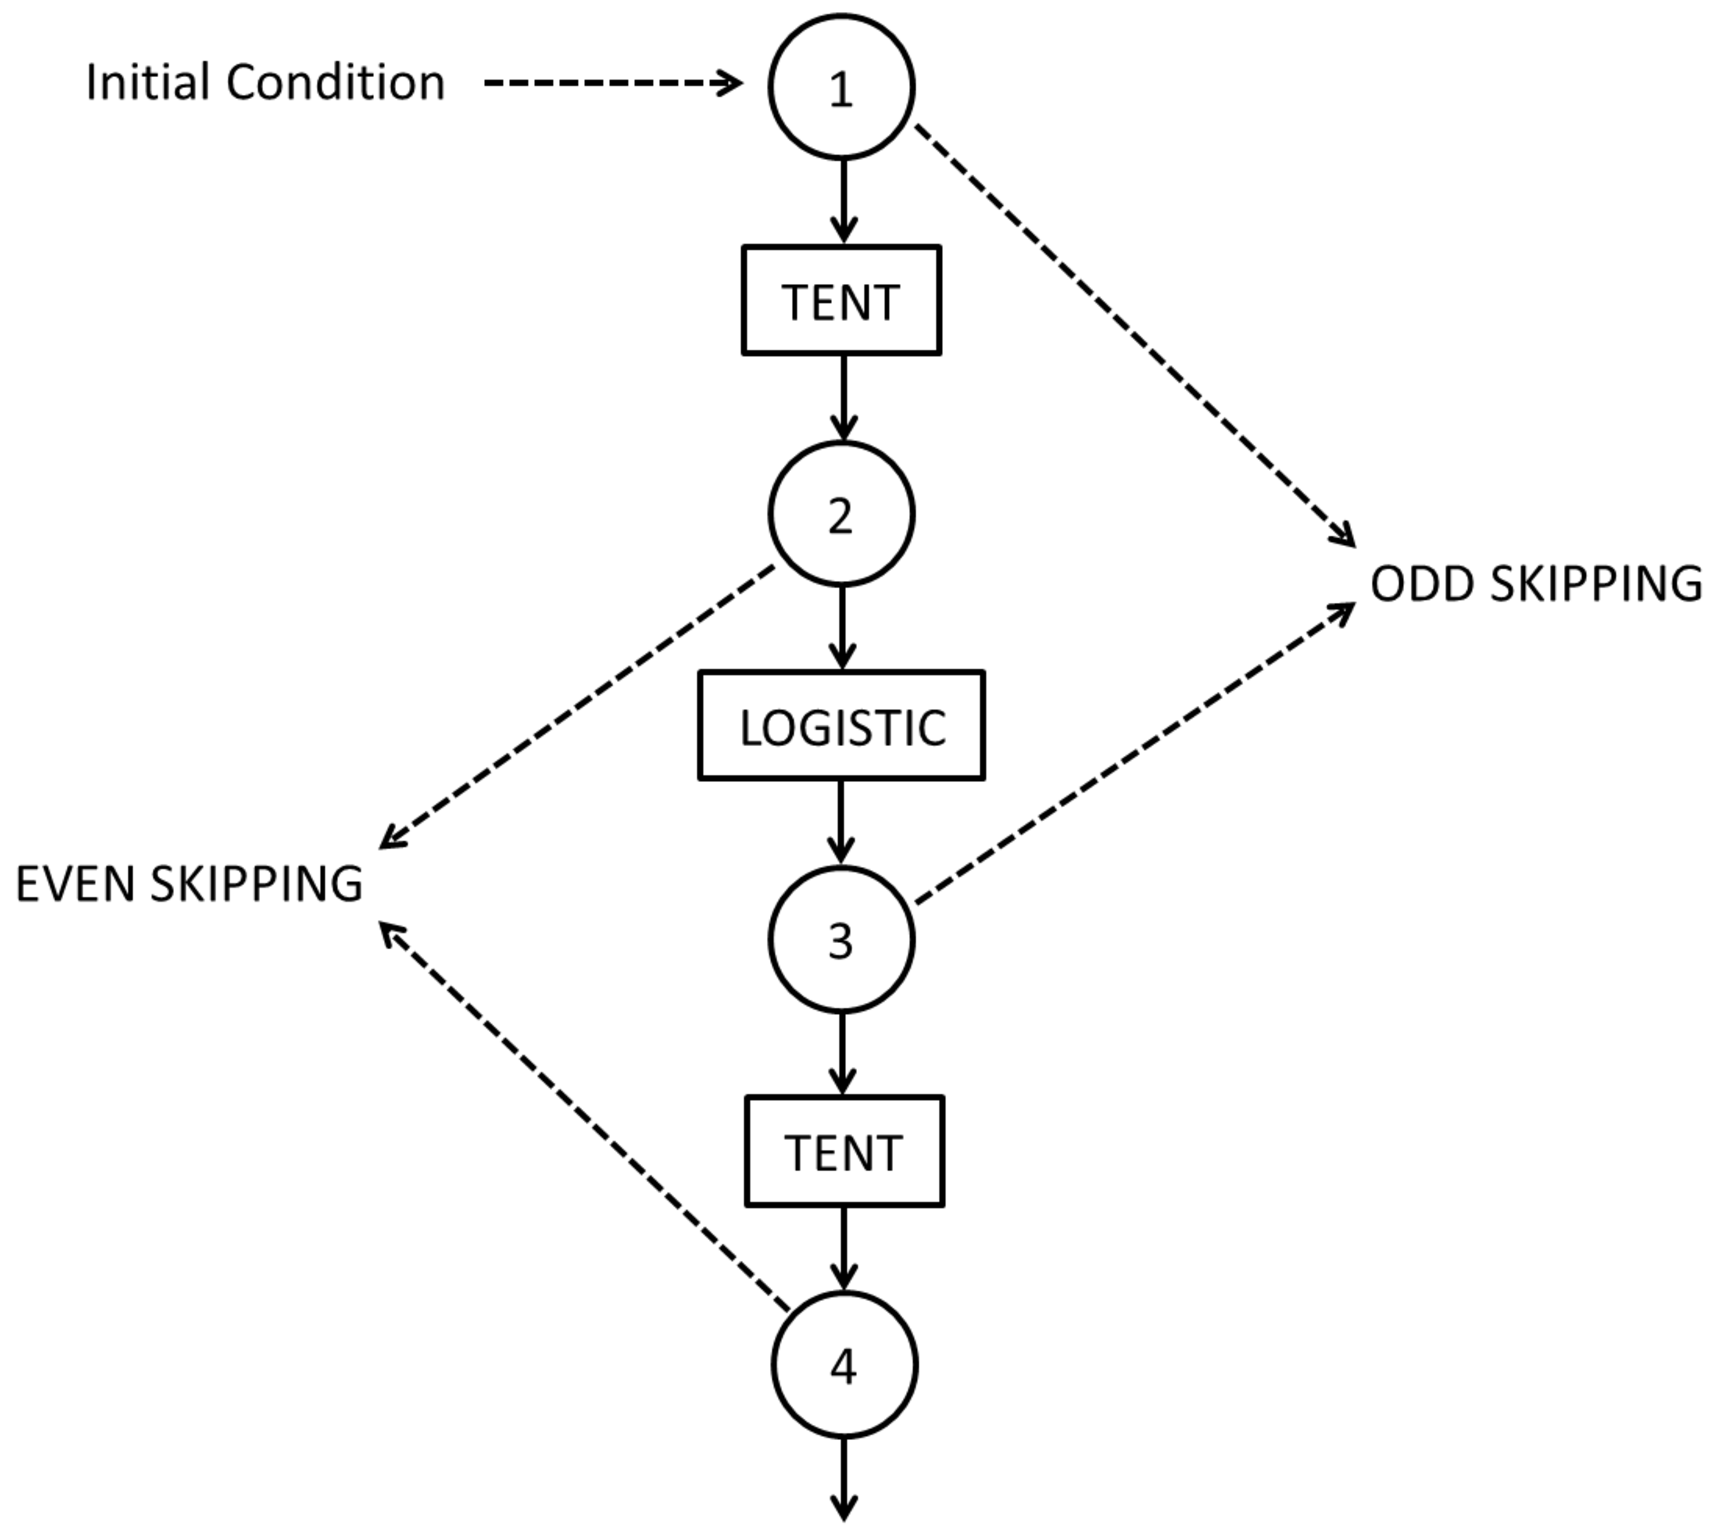
\includegraphics[height=0.4\textheight]{SwitchParImpar}
	\caption{Sequential switching between Tent and Logistic maps. In the figure are also shown even and odd skipping strategies} \label{fig:seq}
\end{figure}
%%%%%%%%%%%%%%%%%%%%%%%%%%
%%%%%%%%%%%%%%%%%%%%%%%%%%% Fig.2

%\begin{figure}
%	\includegraphics[width=0.3\textwidth]{Hval_tentB10}
%	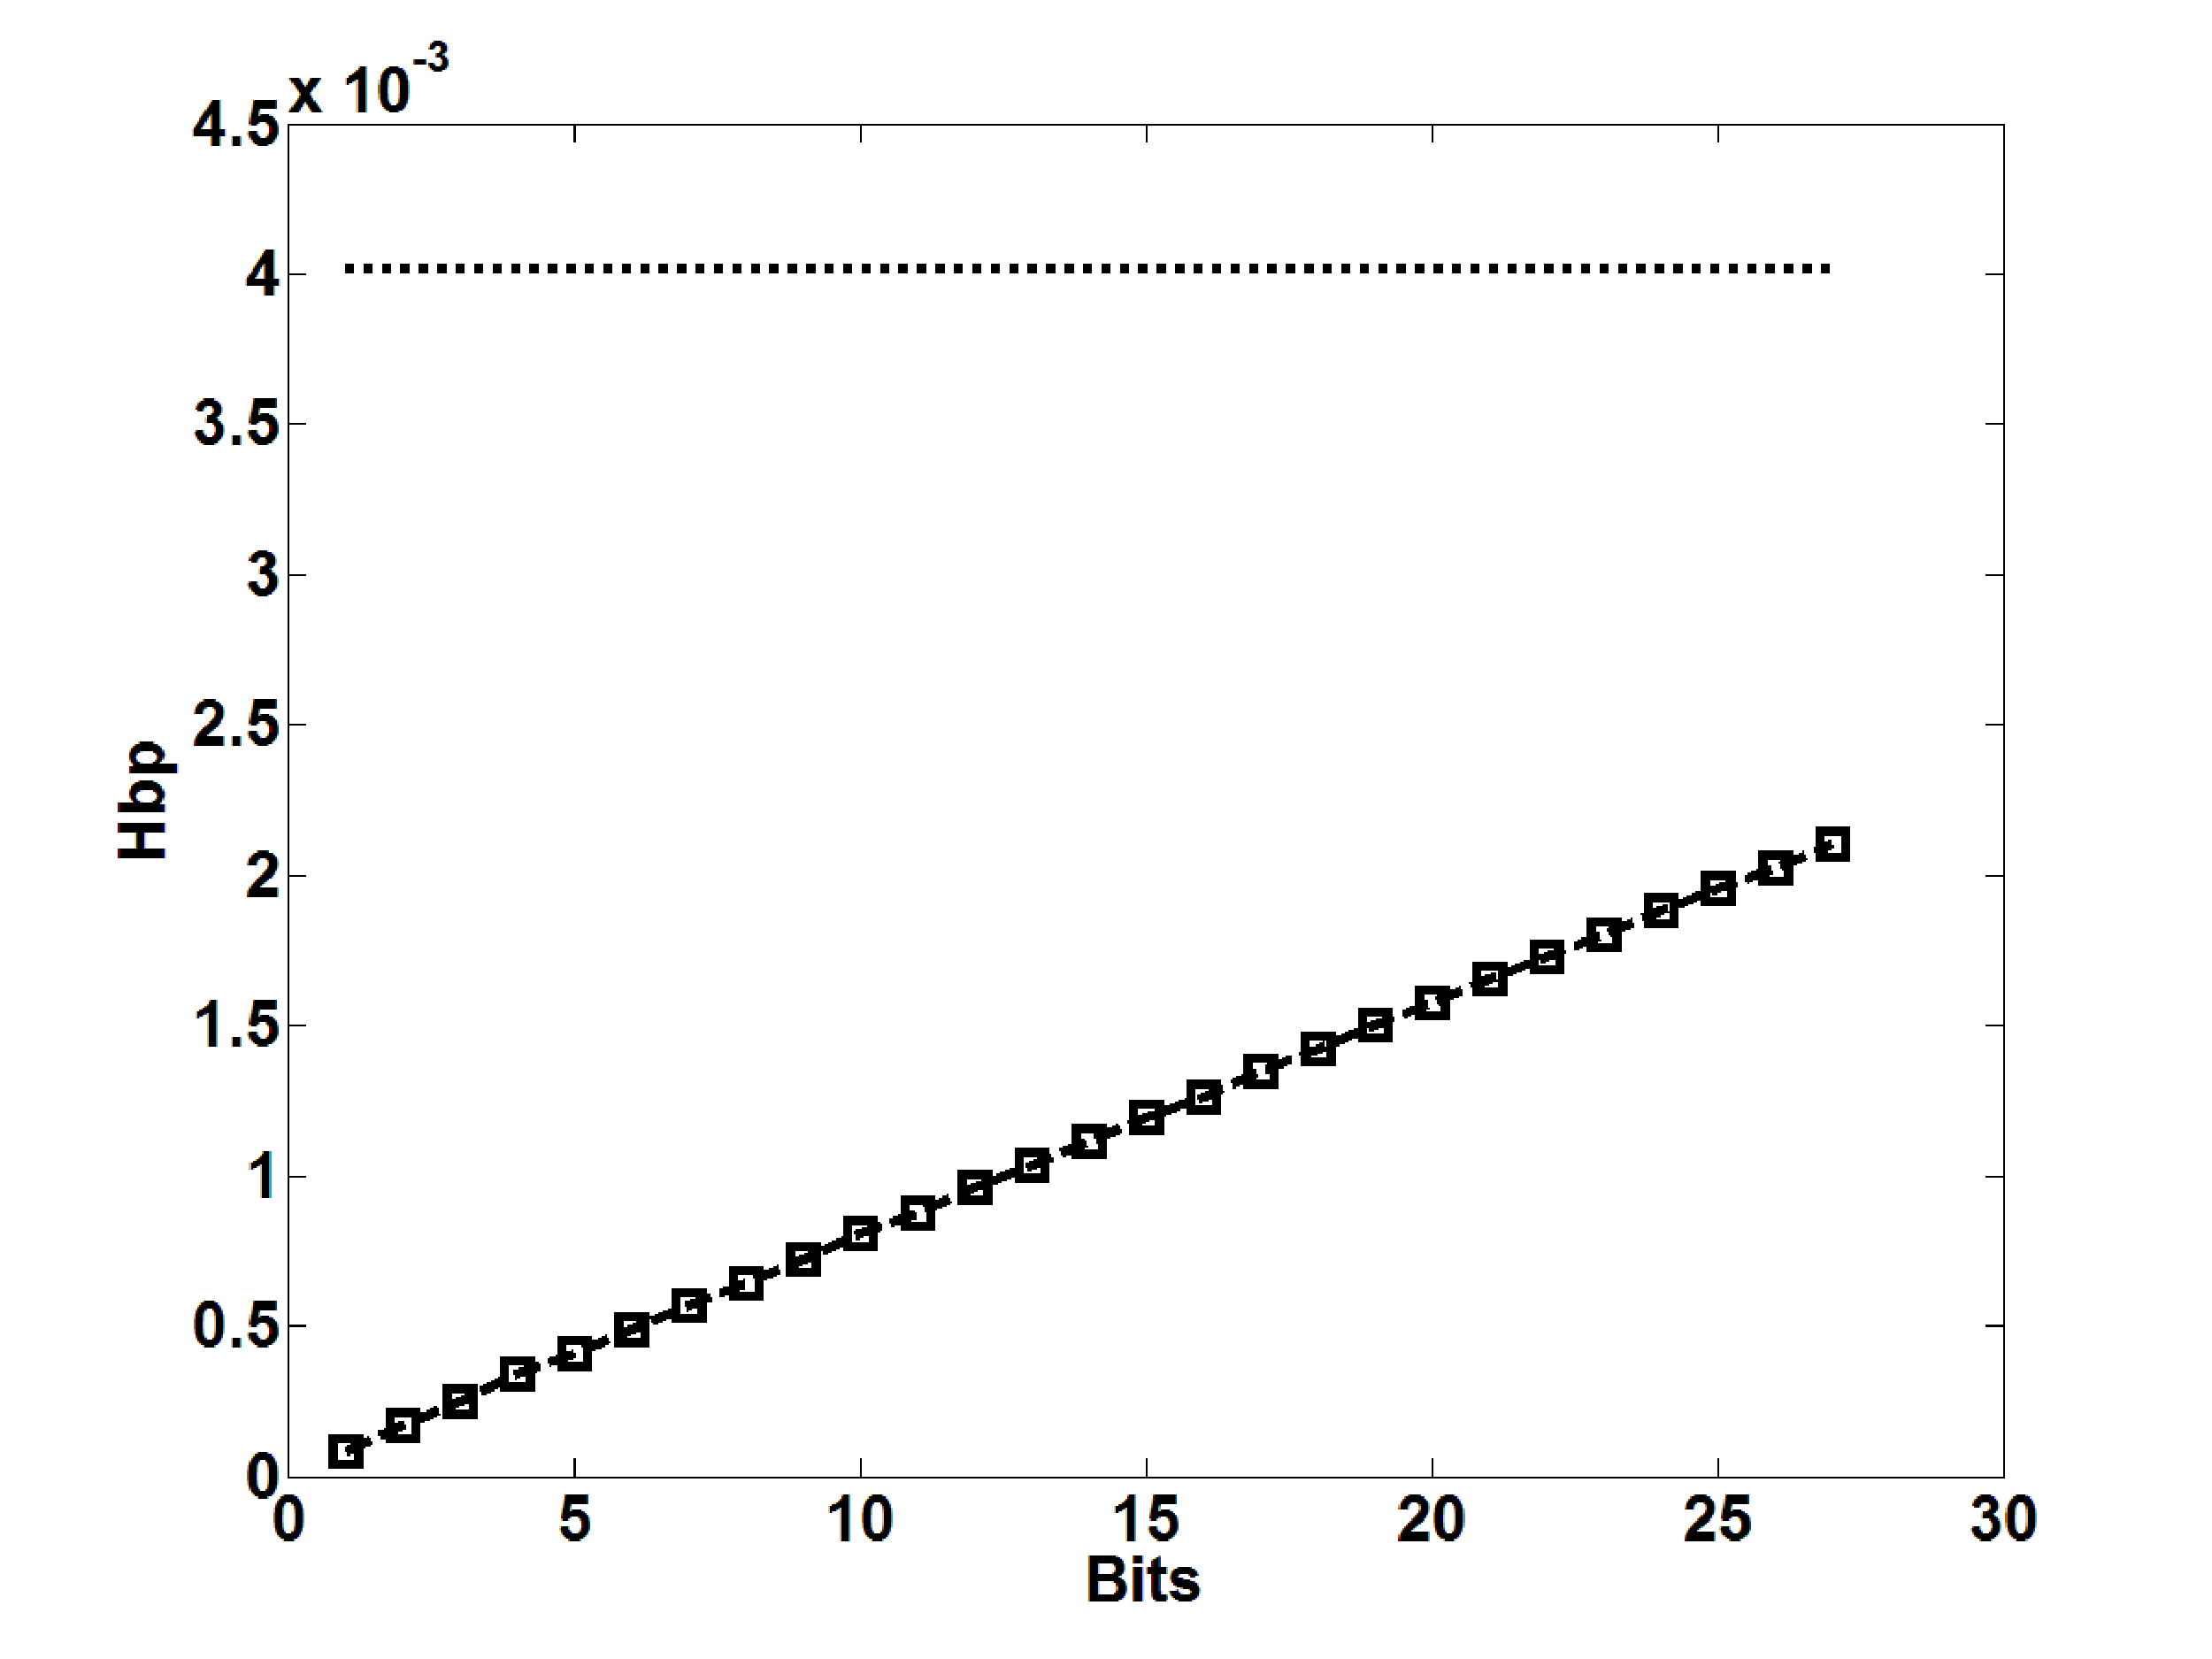
\includegraphics[width=0.3\textwidth]{Hbp_tentB10}
%	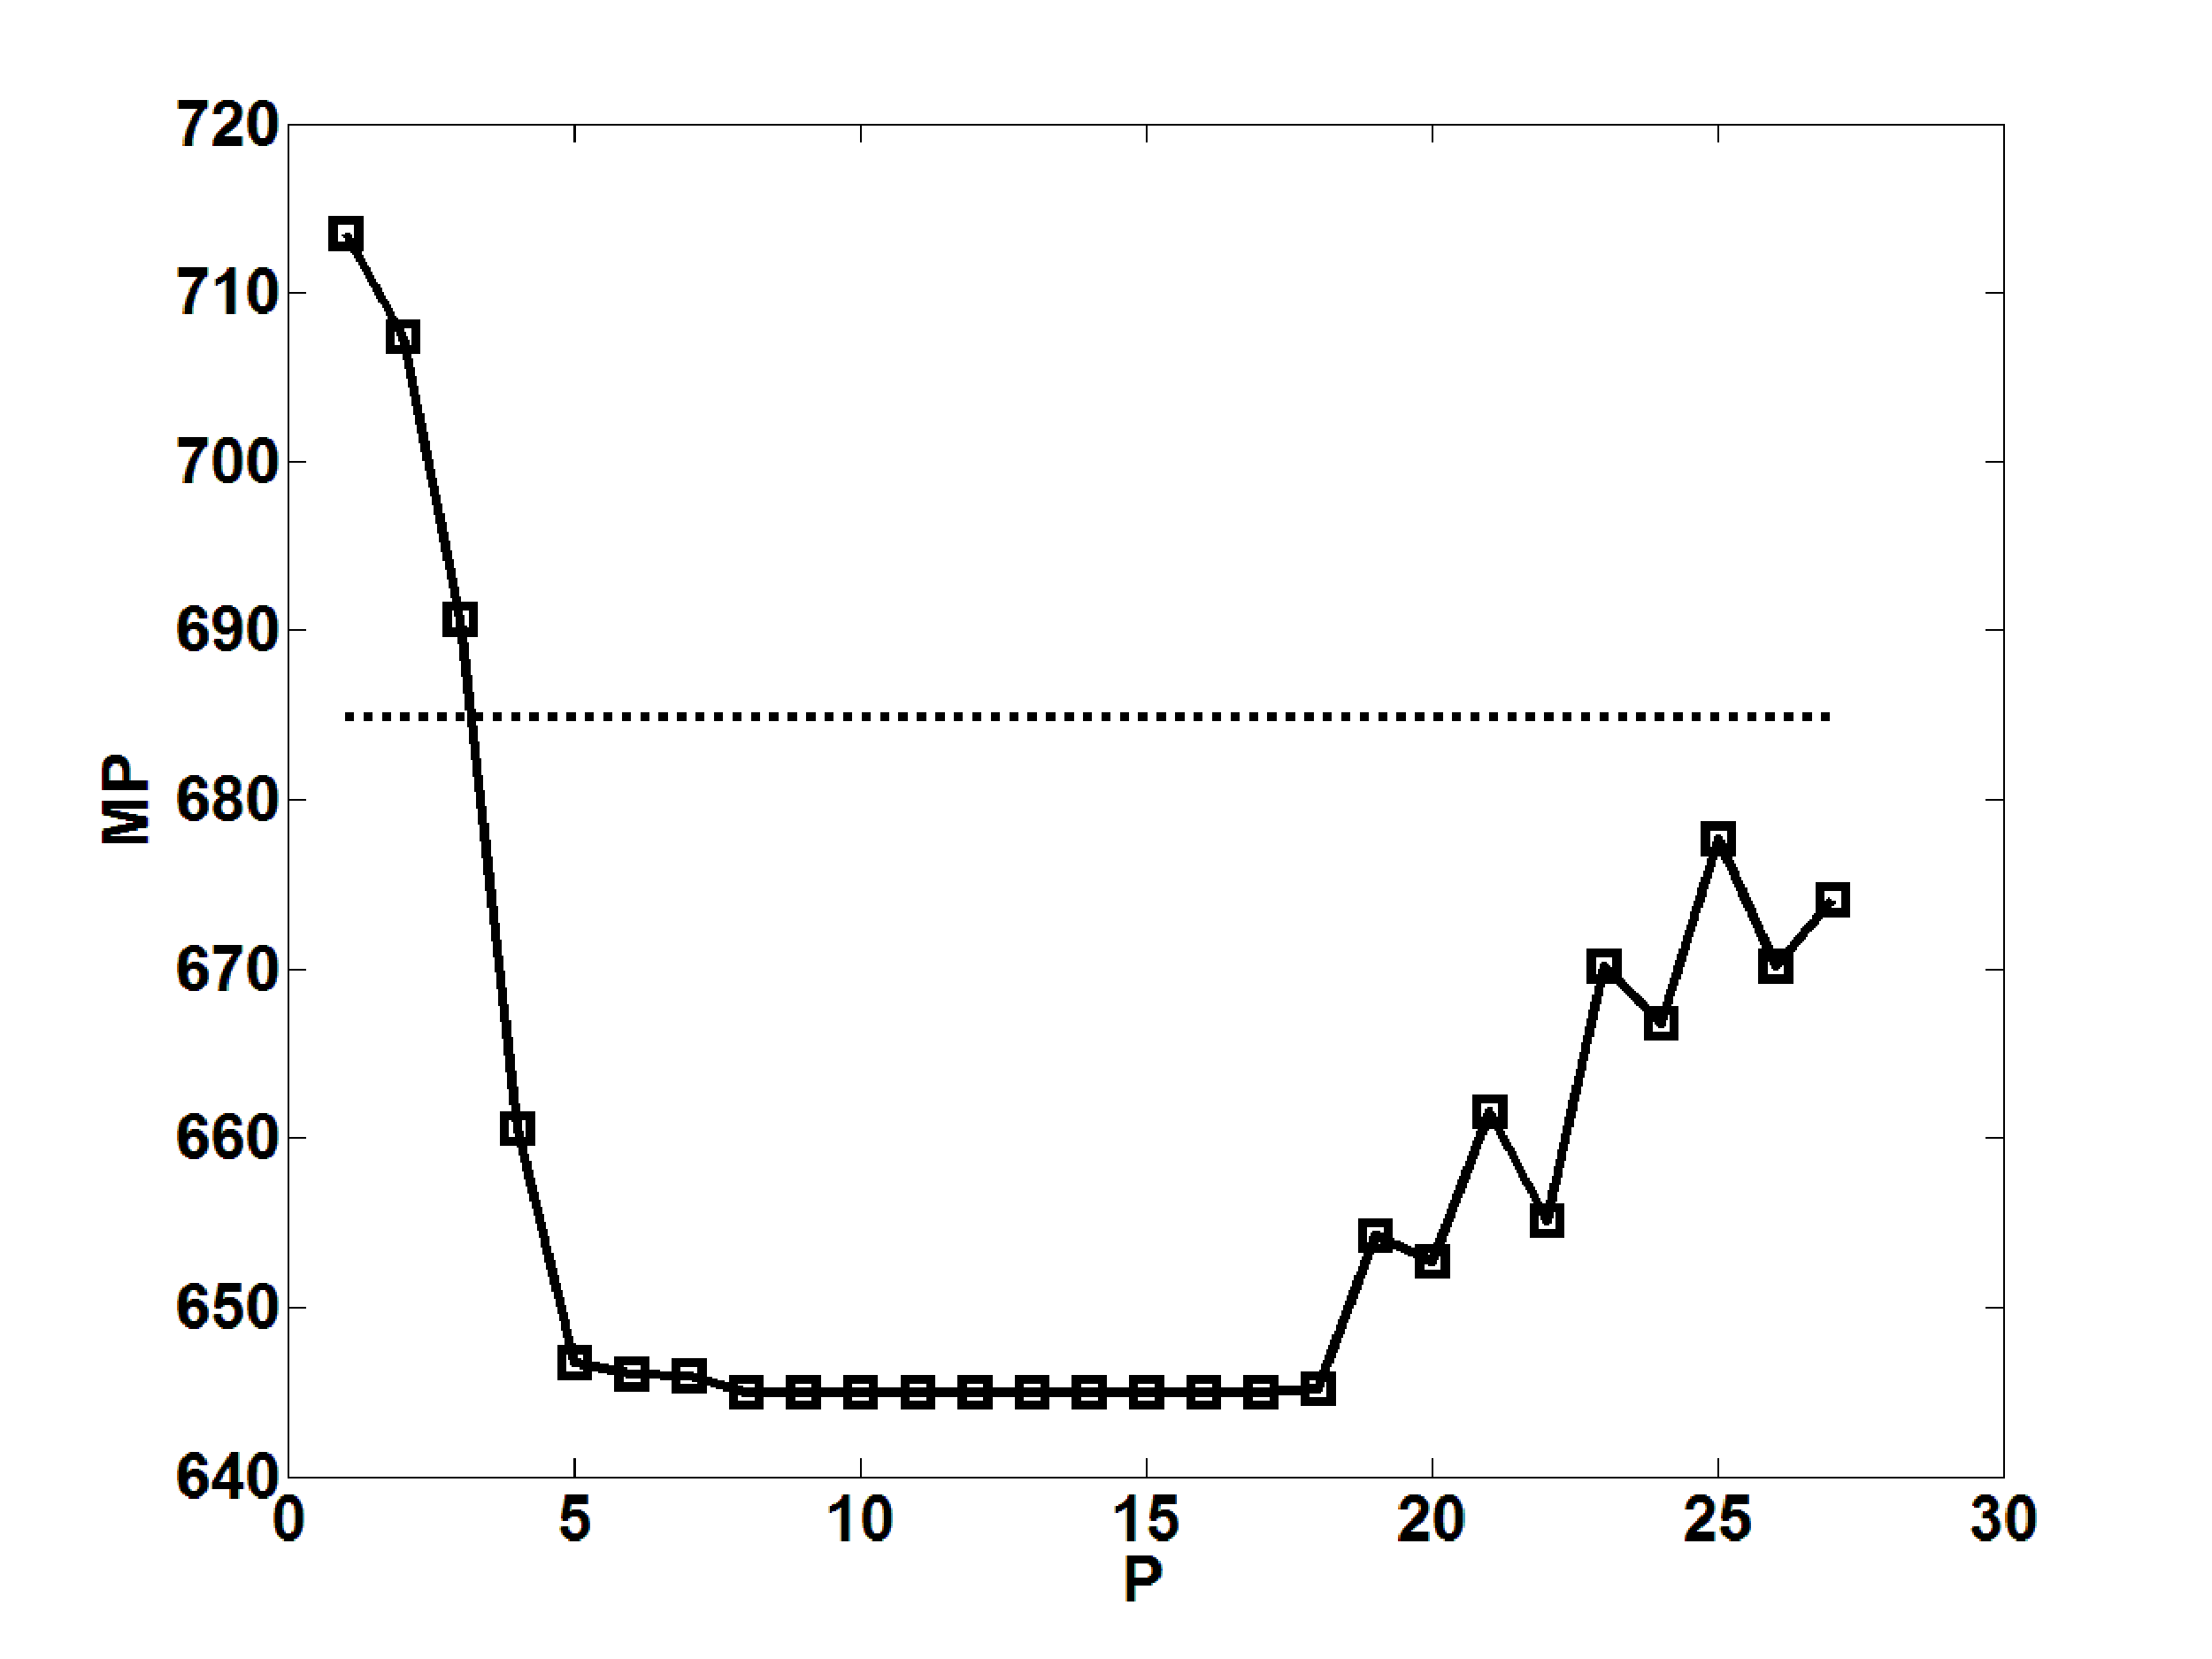
\includegraphics[width=0.3\textwidth]{Miss_tentB10}
%	\includegraphics[width=0.3\textwidth]{HvalHbp_tentB10}
%	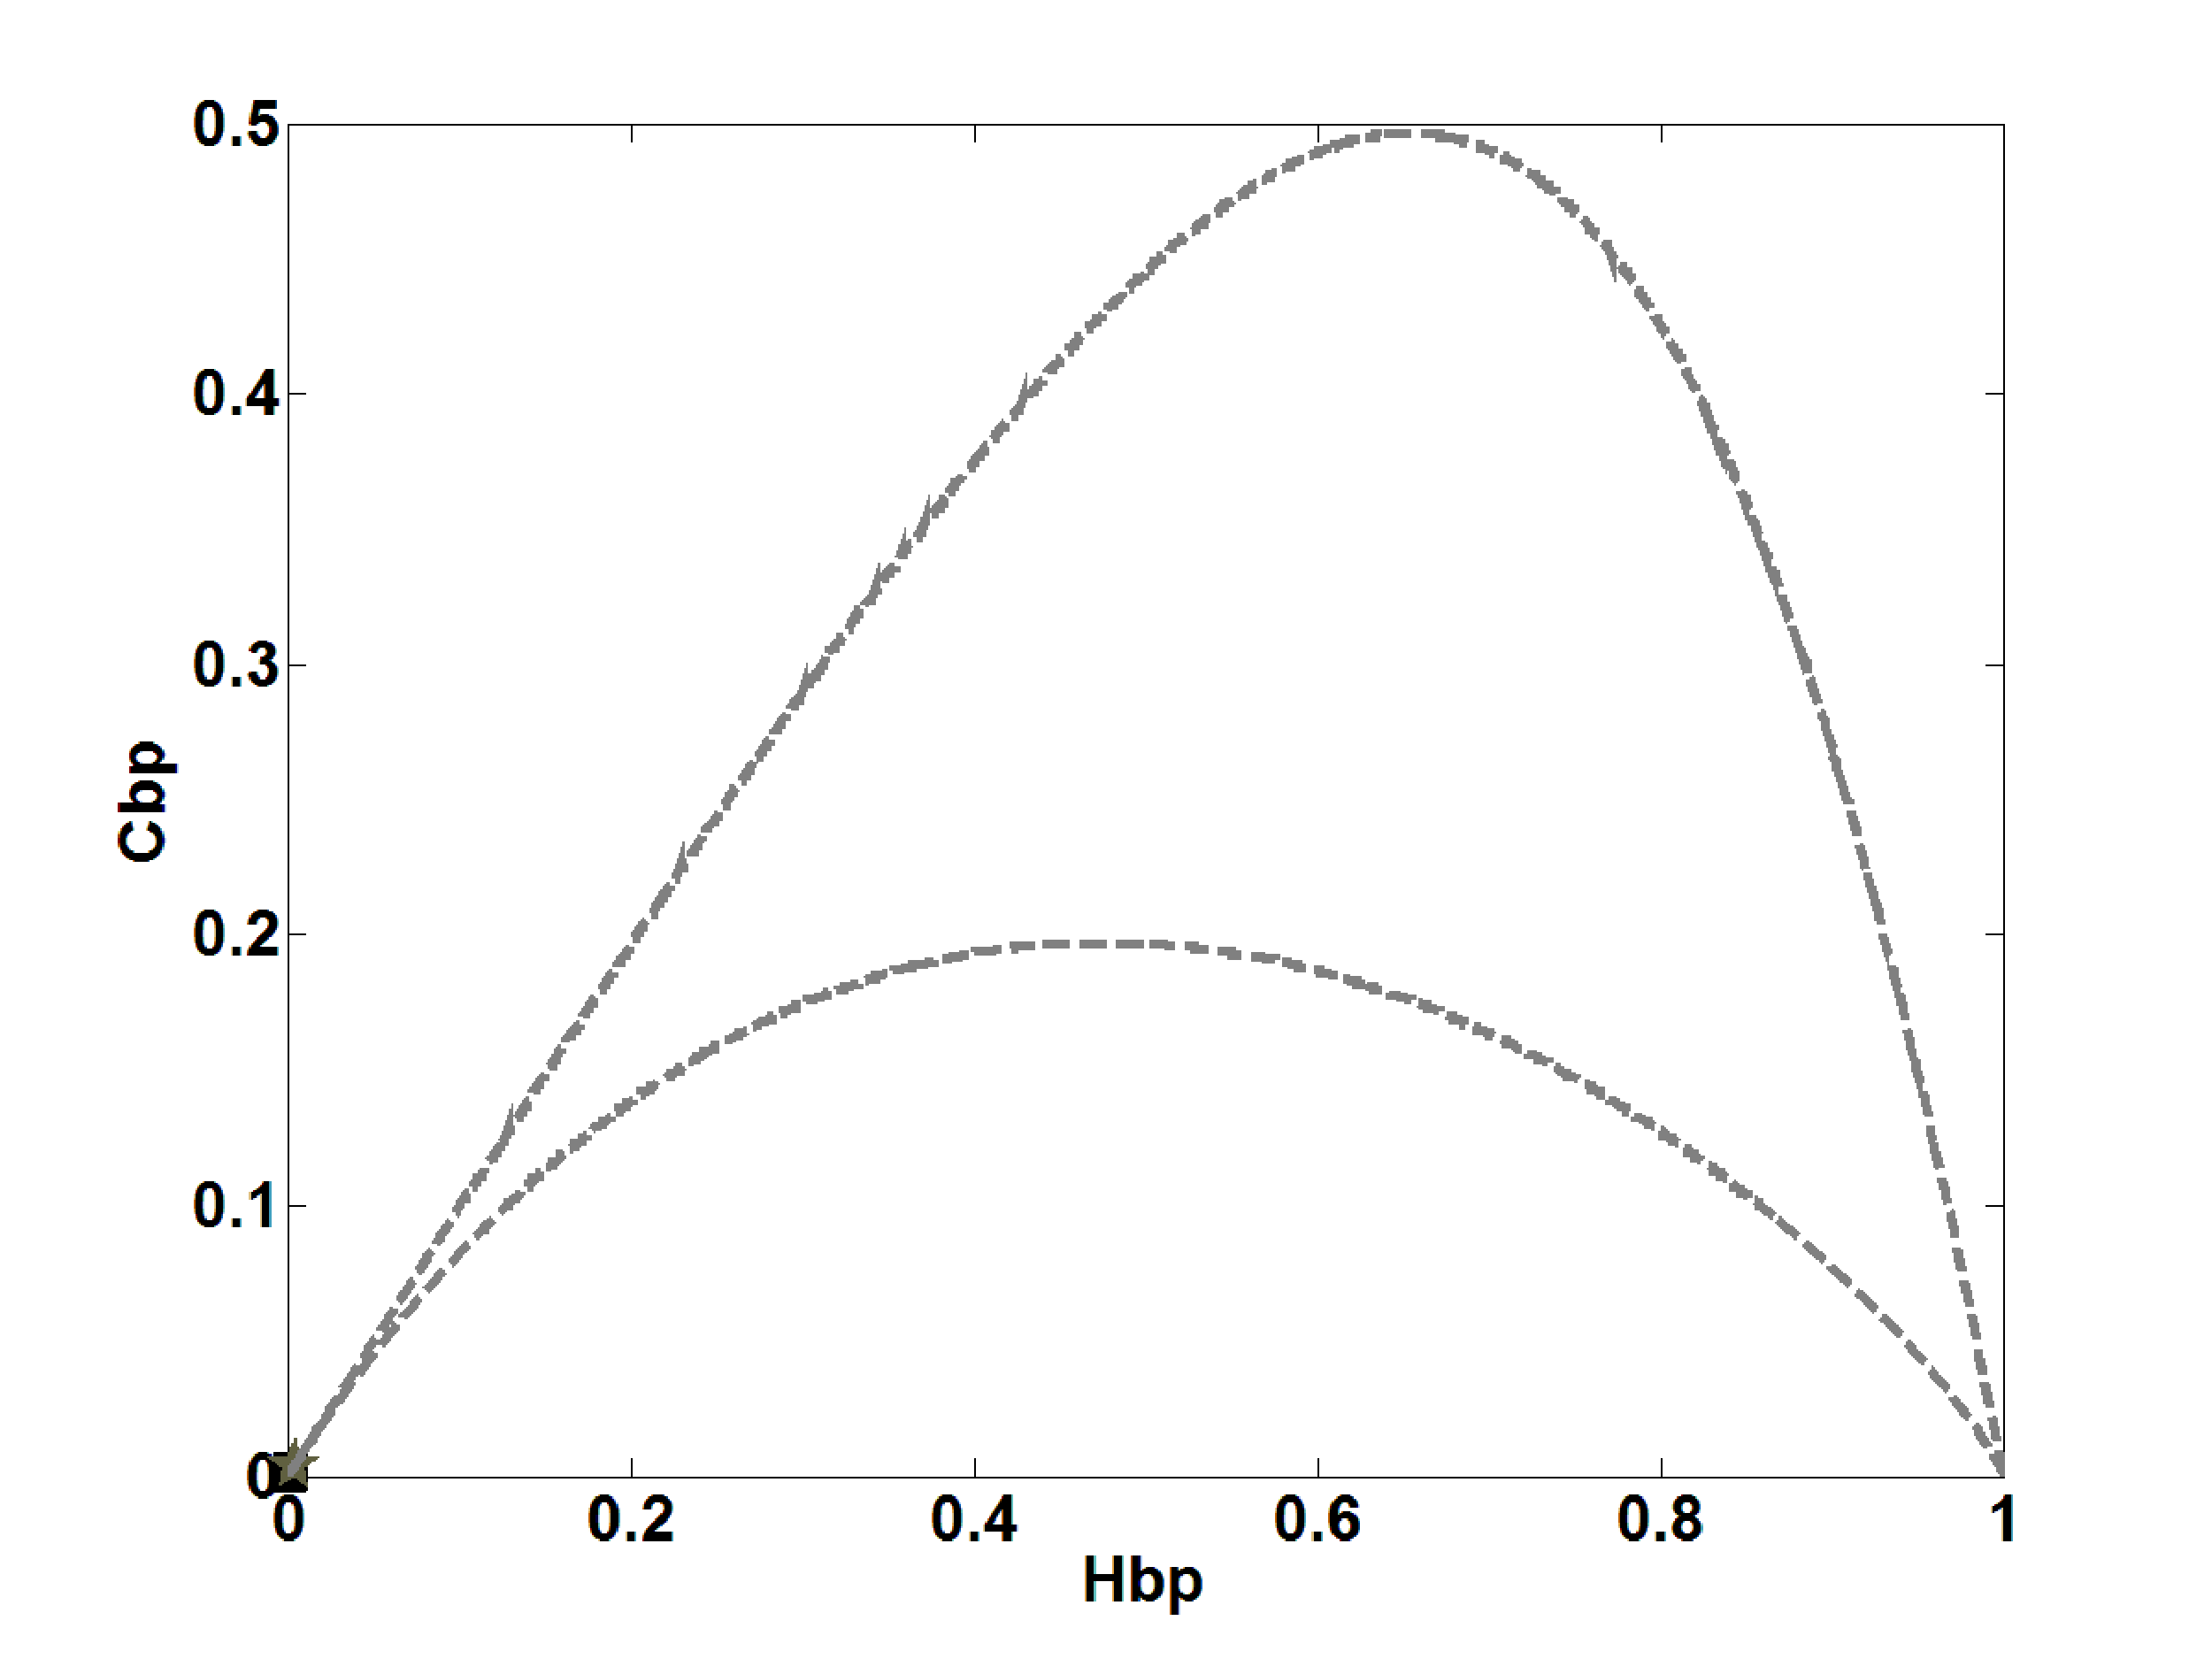
\includegraphics[width=0.3\textwidth]{HbpCbp_tentB10}
%	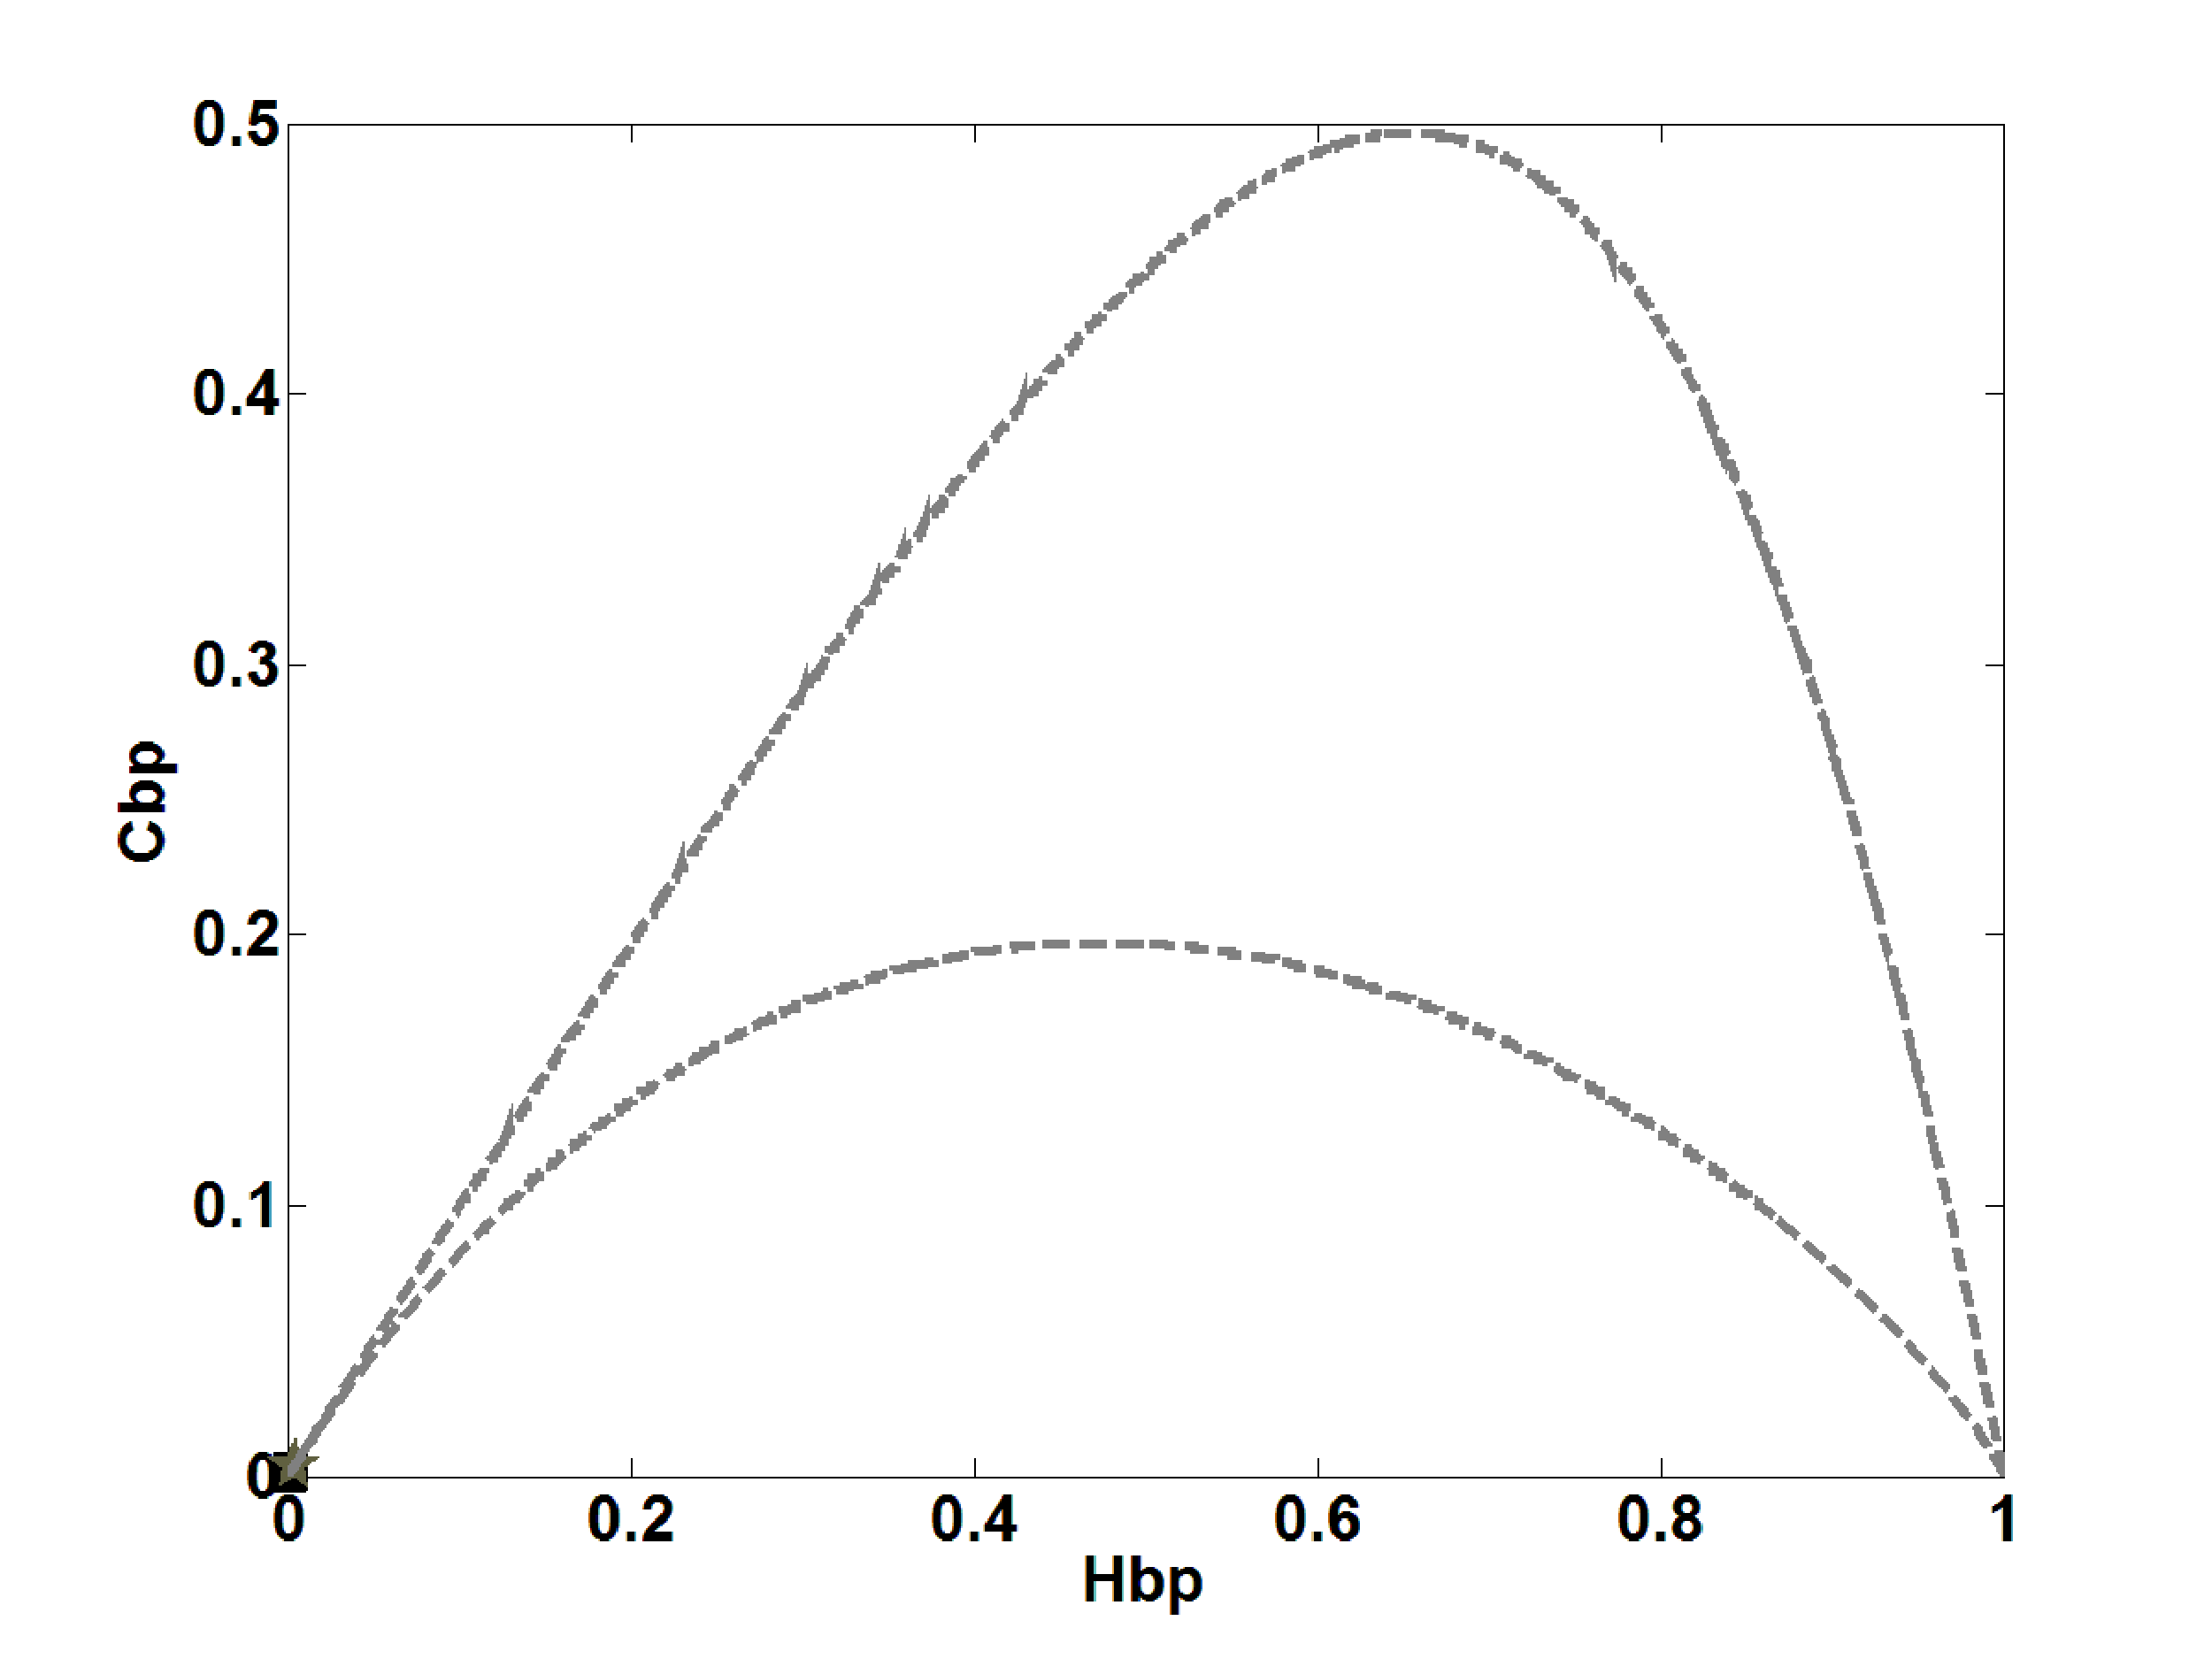
\includegraphics[width=0.3\textwidth]{HbpCbp_tentB2}
%	\caption{Statistical properties of the Tent map using different numerical representations. Figures (a) to(e) correspond to decimal representation: (a) $H_{hist}$ vs $P$ (b) $H_{BP}$ vs $P$ (c) Number of missing ordering patterns $MP$ vs $P$. In Figures (a) to (c) dashed line correspond to floating point numbers. (d) representation in the $H_{hist},H_{BP}$ plane in the the decimal numerical system.  The star represents the state for floating points numbers. (e) representation in the $H_{BP},C_{BP}$ plane.  The star represents the state for floating points numbers. (f) representation in the $H_{BP},C_{BP}$ plane for binary numerical system.  The star represents the state for floating points numbers. } \label{fig:tent}
%\end{figure}

%%%%%%%%%%%%%%%%%%%%%%%%%%
%%%%%%%%%%%%%%%%%%%%%%%%%%% Fig.3
%\begin{figure}
%	\includegraphics[width=0.3\textwidth]{Hval_logisticoB10}
%	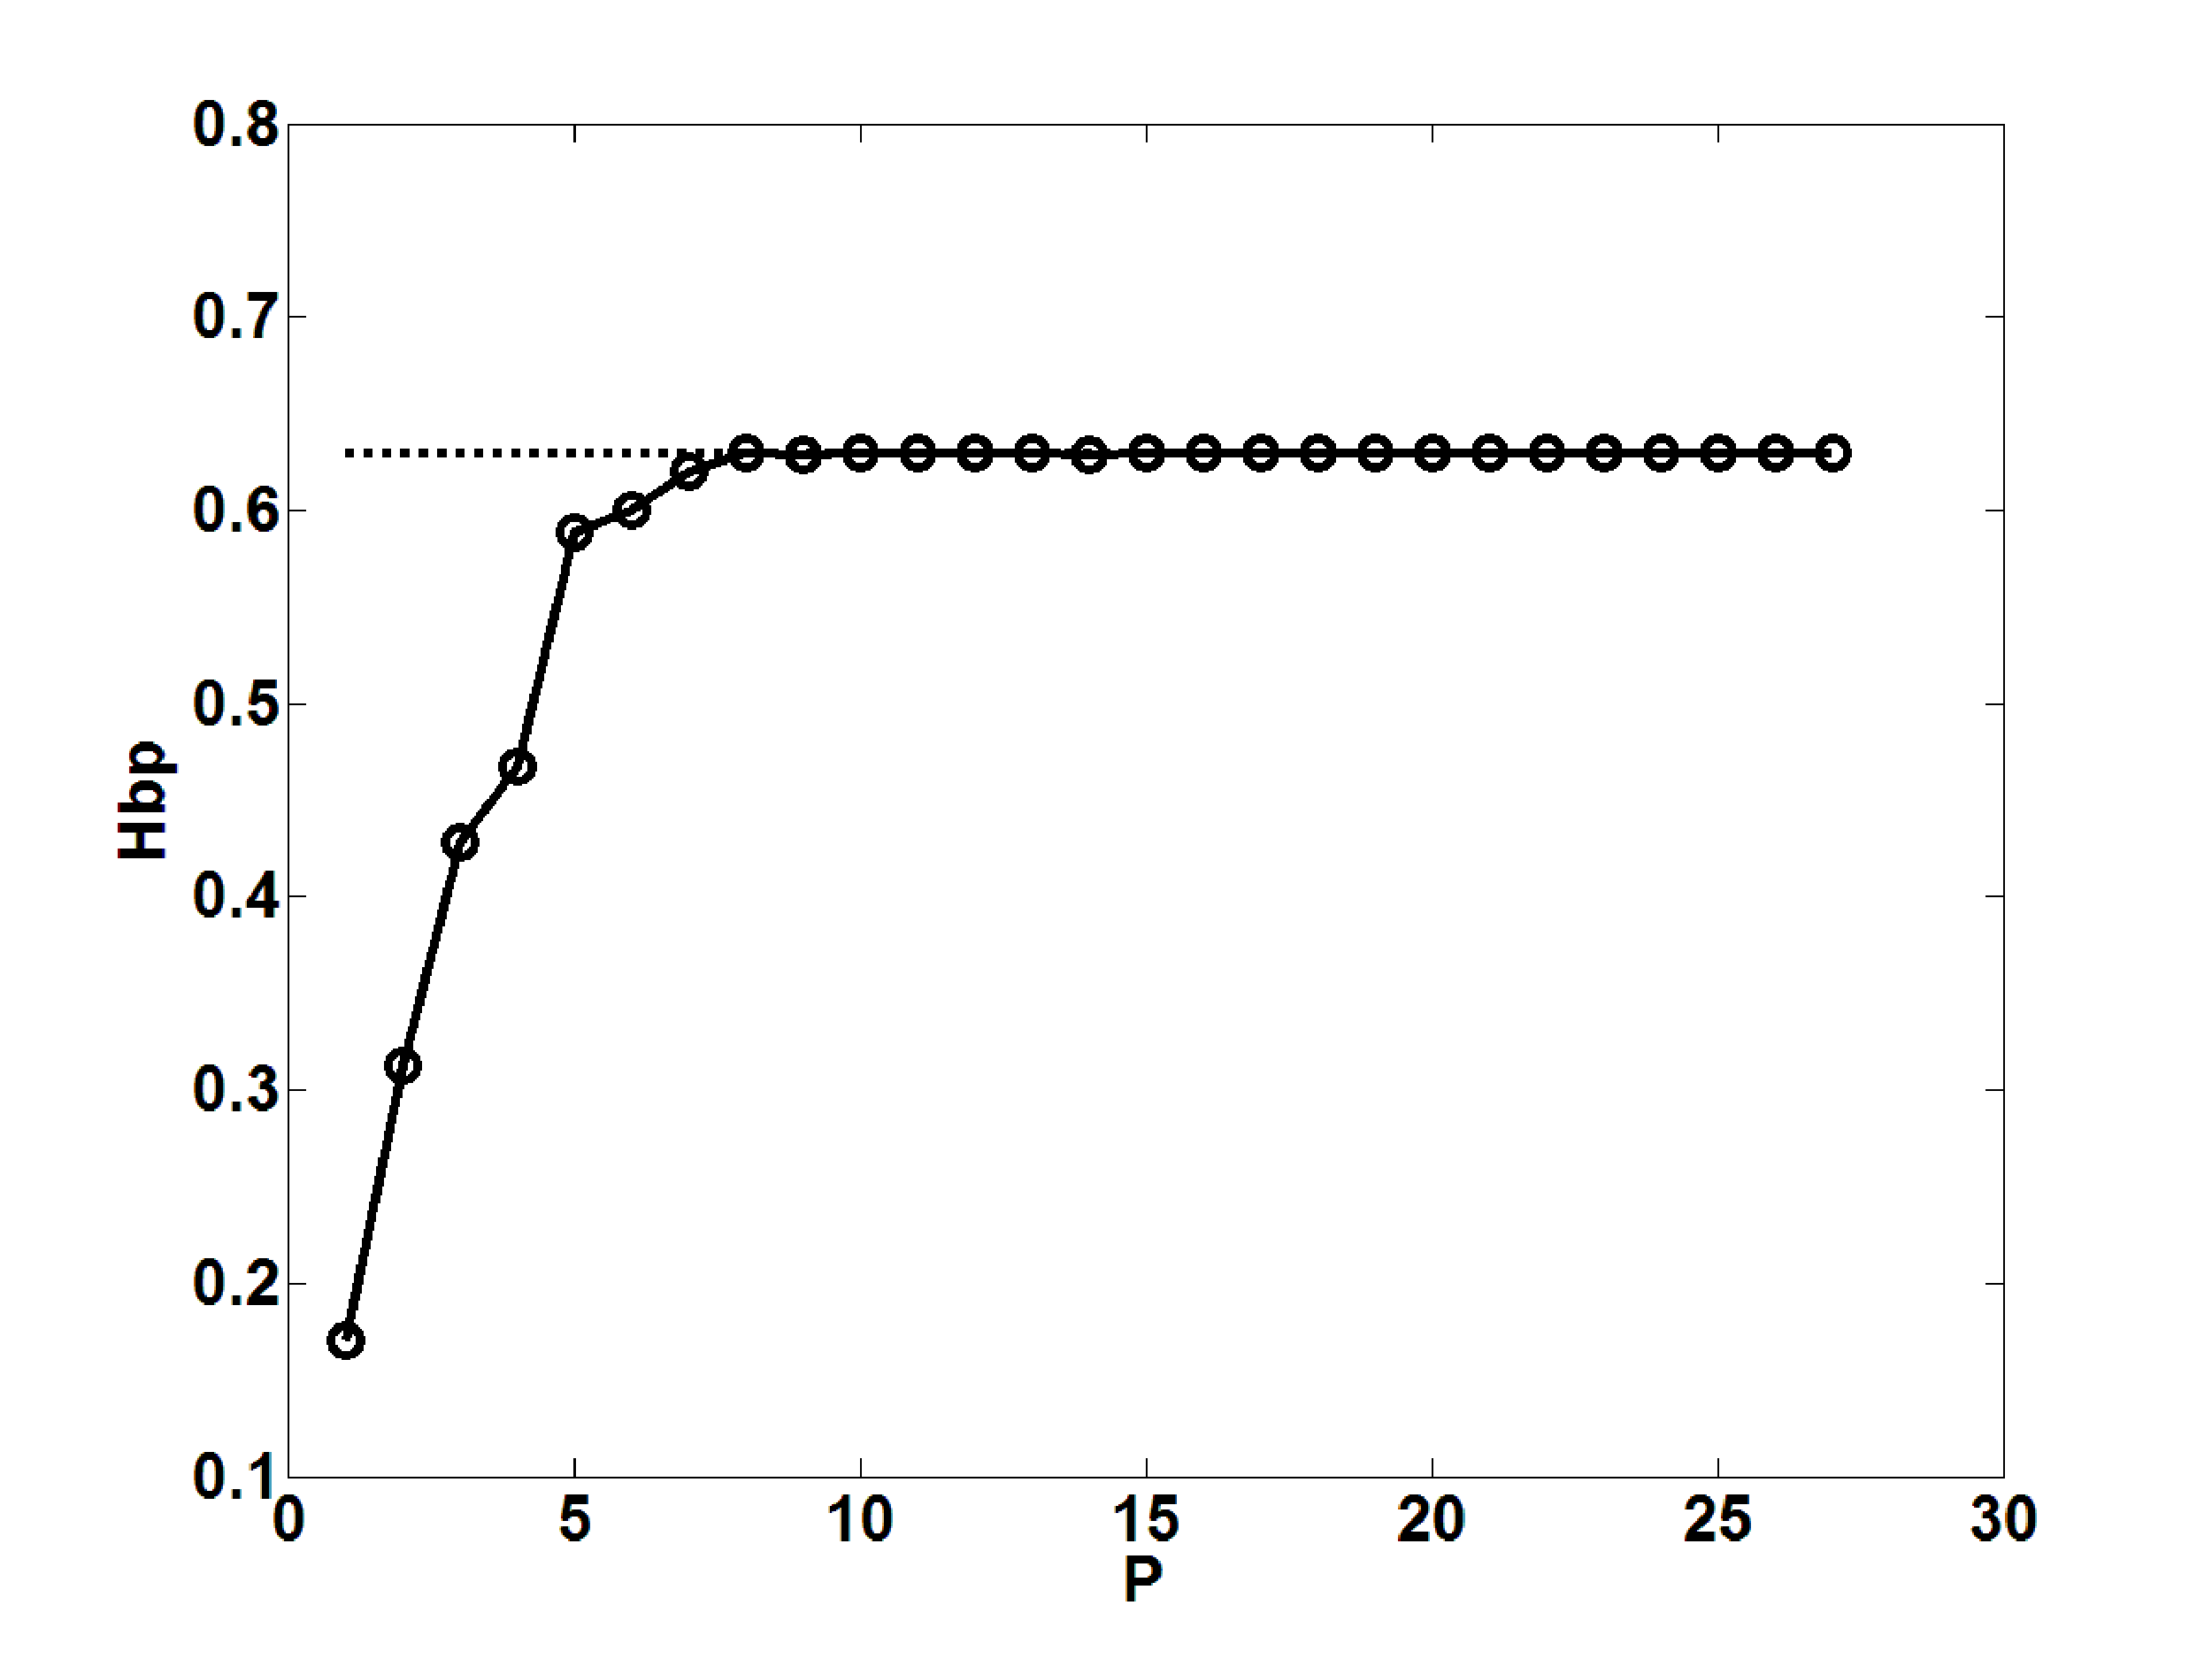
\includegraphics[width=0.3\textwidth]{Hbp_logisticoB10}
%	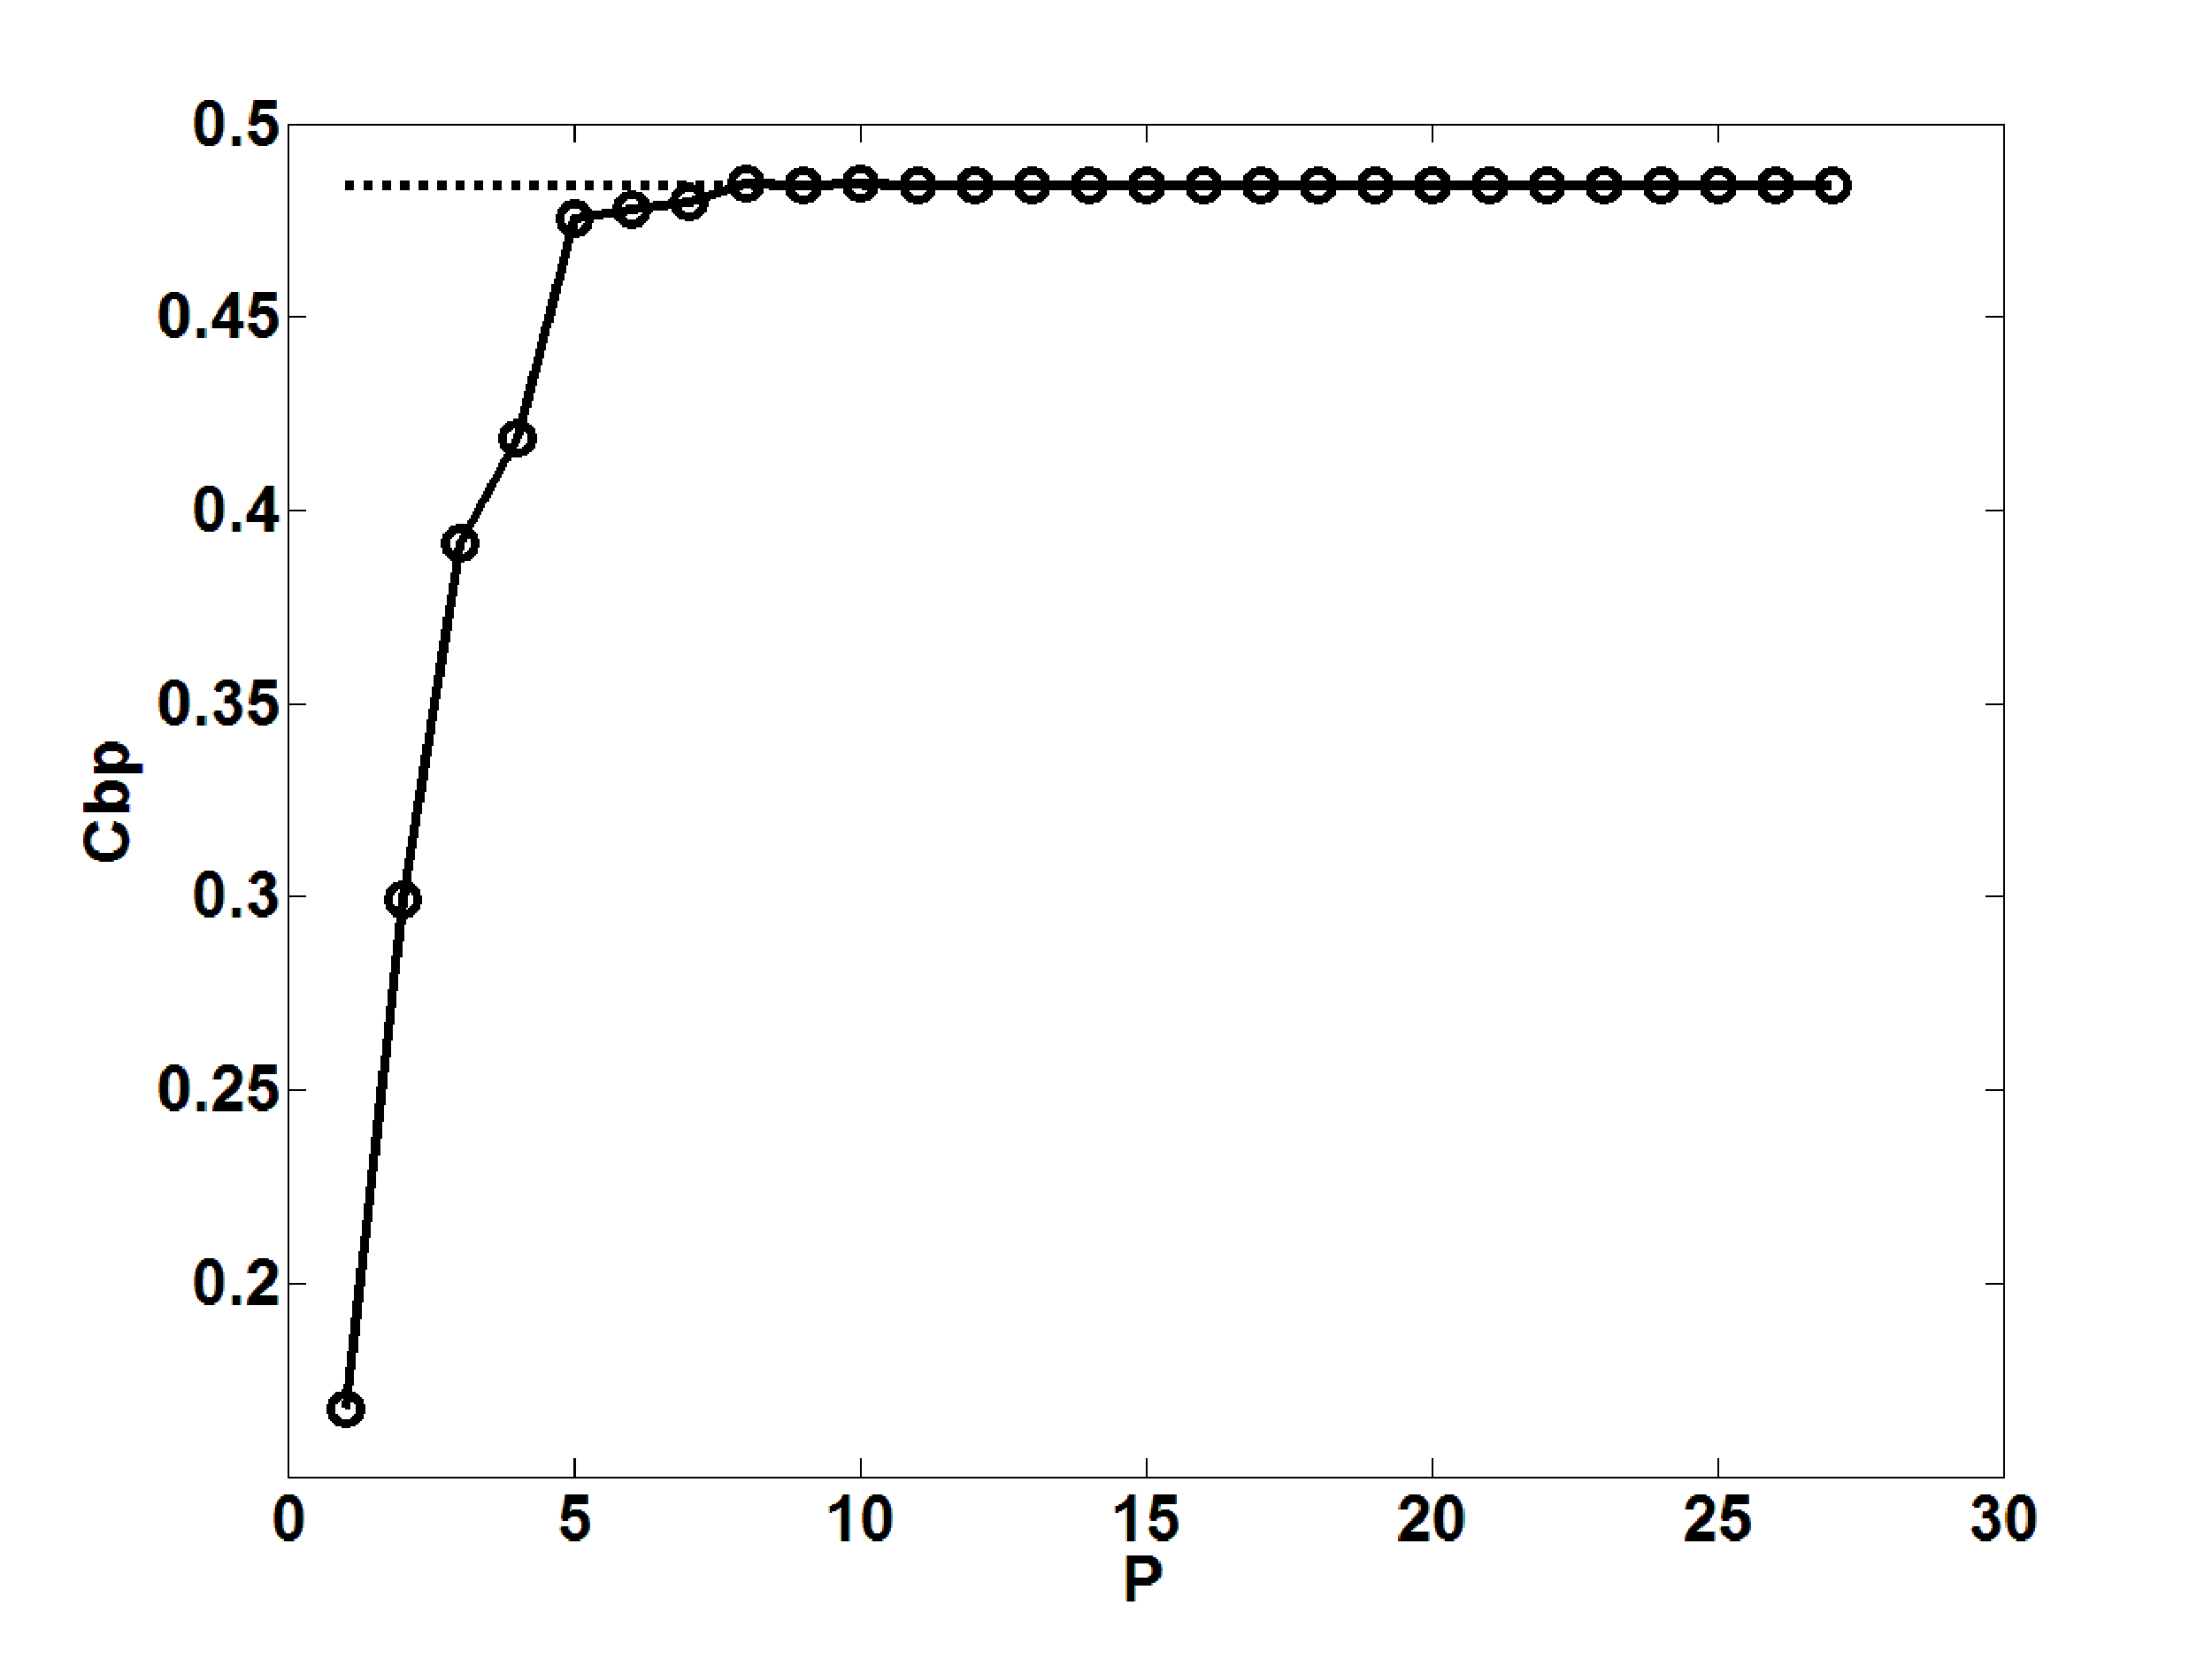
\includegraphics[width=0.3\textwidth]{Cbp_logisticoB10}
%	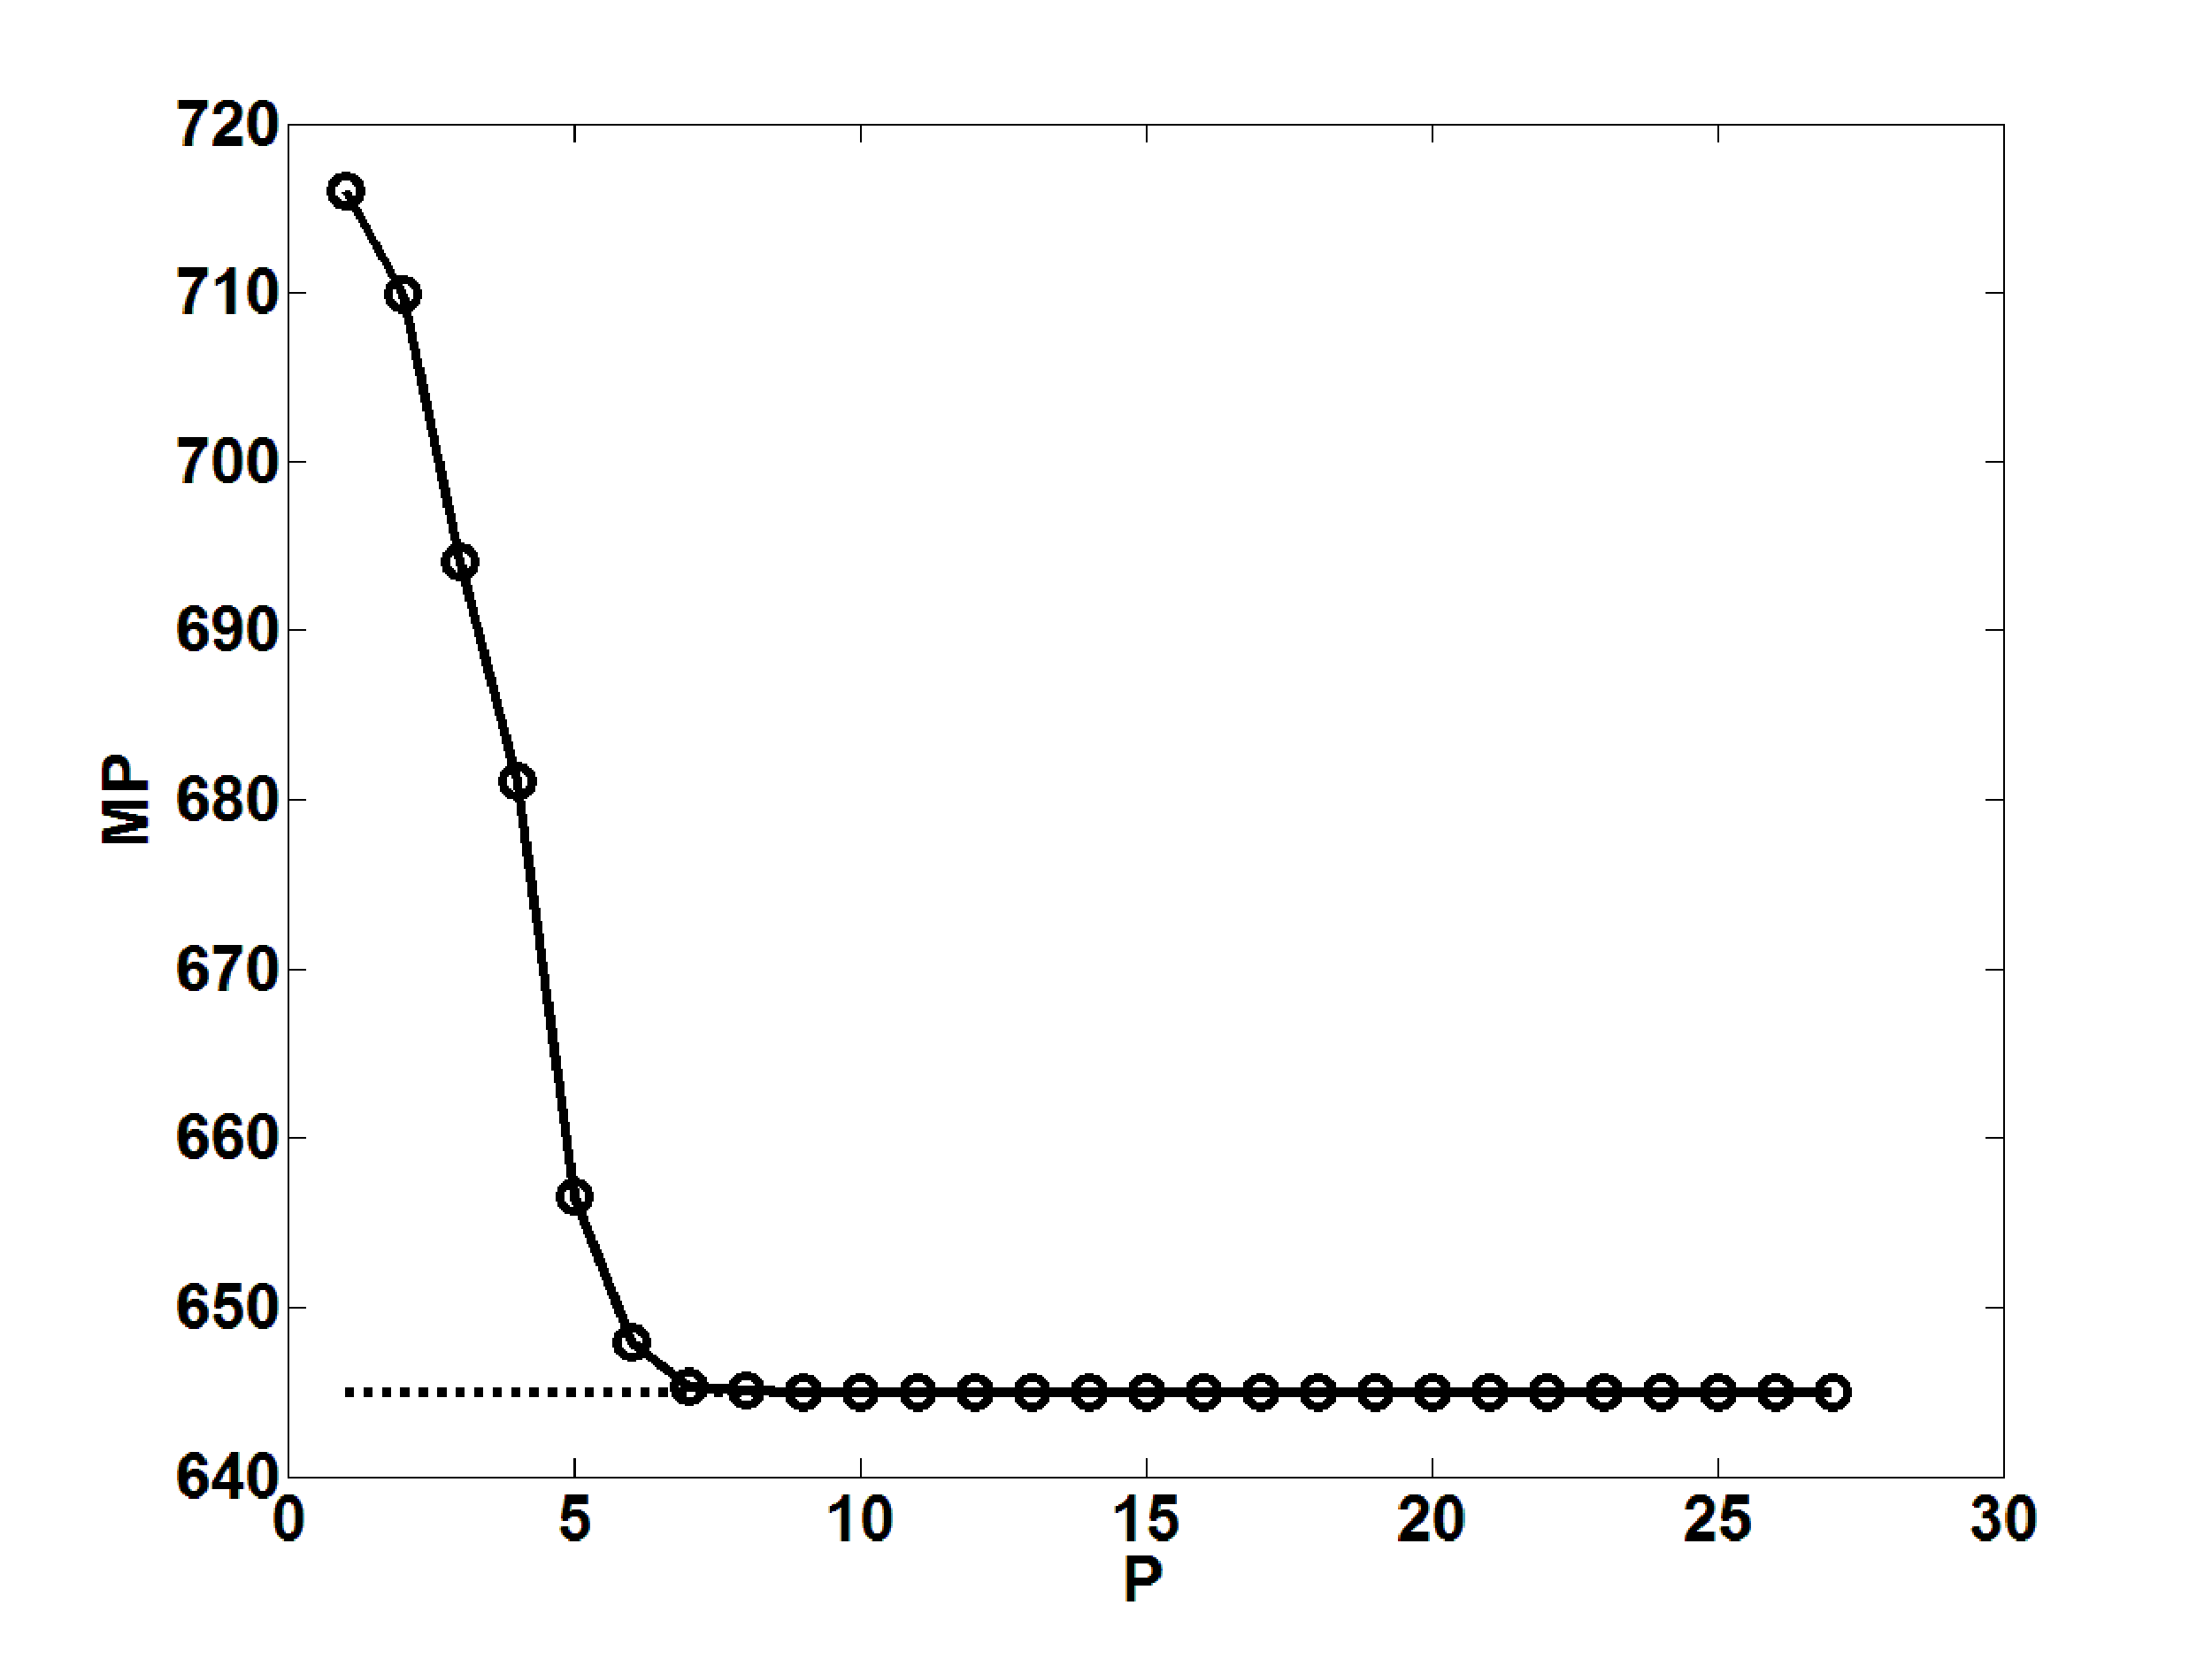
\includegraphics[width=0.3\textwidth]{Miss_logisticoB10}
%	\includegraphics[width=0.3\textwidth]{HvalHbp_logisticoB10}
%	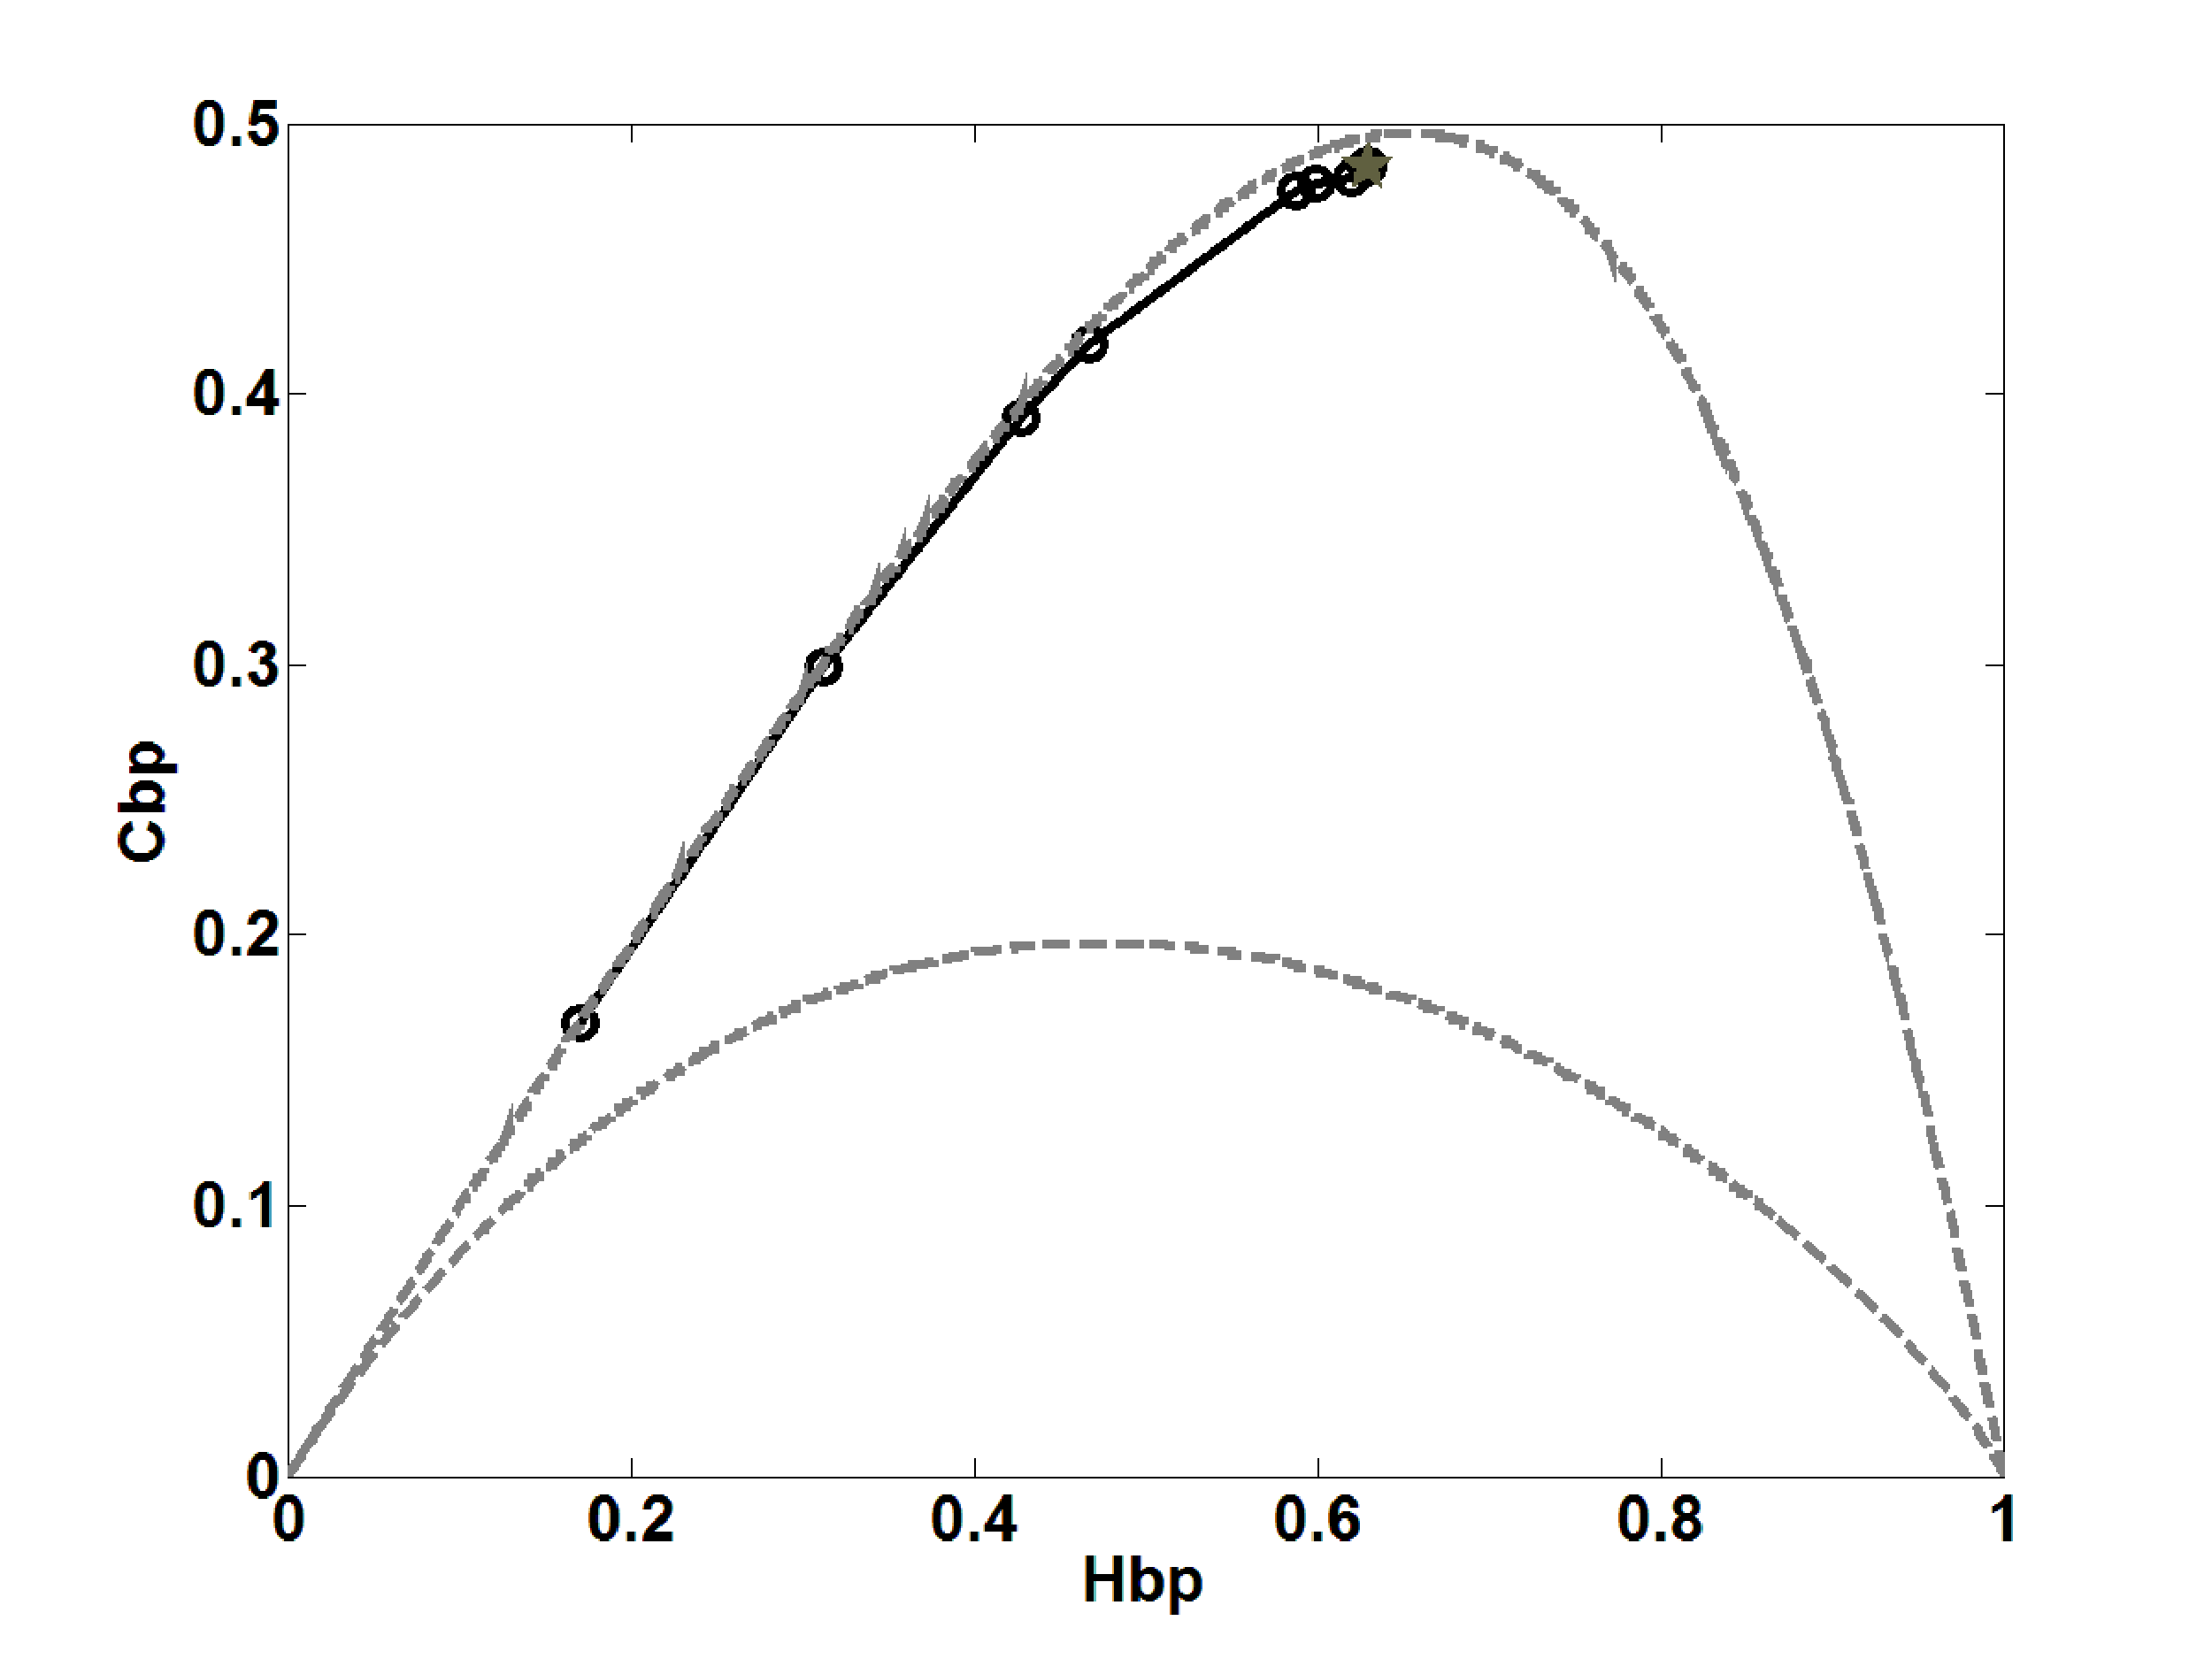
\includegraphics[width=0.3\textwidth]{HbpCbp_logisticoB10}
%	\caption{Statistical properties of the LOG map using different numerical representations. Figures (a) to(f) correspond to decimal representation: (a) $H_{hist}$ vs $P$ (b) $H_{BP}$ vs $P$ (c) $C_{BP}$ vs $P$ (d) Number of missing ordering patterns $MP$ vs $P$. In Figures (a) to (d) dashed line correspond to floating point numbers. (d) representation in the $H_{hist},H_{BP}$ plane in the the decimal numerical system.  The star represents the state for floating points numbers. (e) representation in the $H_{hist},H_{BP}$ plane. The star represents the state for floating point numbers; (f) representation in the $H_{BP},C_{BP}$ plane.  The star represents the state for floating points numbers. (f) representation in the $H_{BP},C_{BP}$ plane for binary numerical system.  The star represents the state for floating points numbers. } \label{fig:LOGdecimal}
%\end{figure}
%%%%%%%%%%%%%%%%%%%%%%%%%%
%%%%%%%%%%%%%%%%%%%%%%%%%%% Fig.4
\begin{figure}
	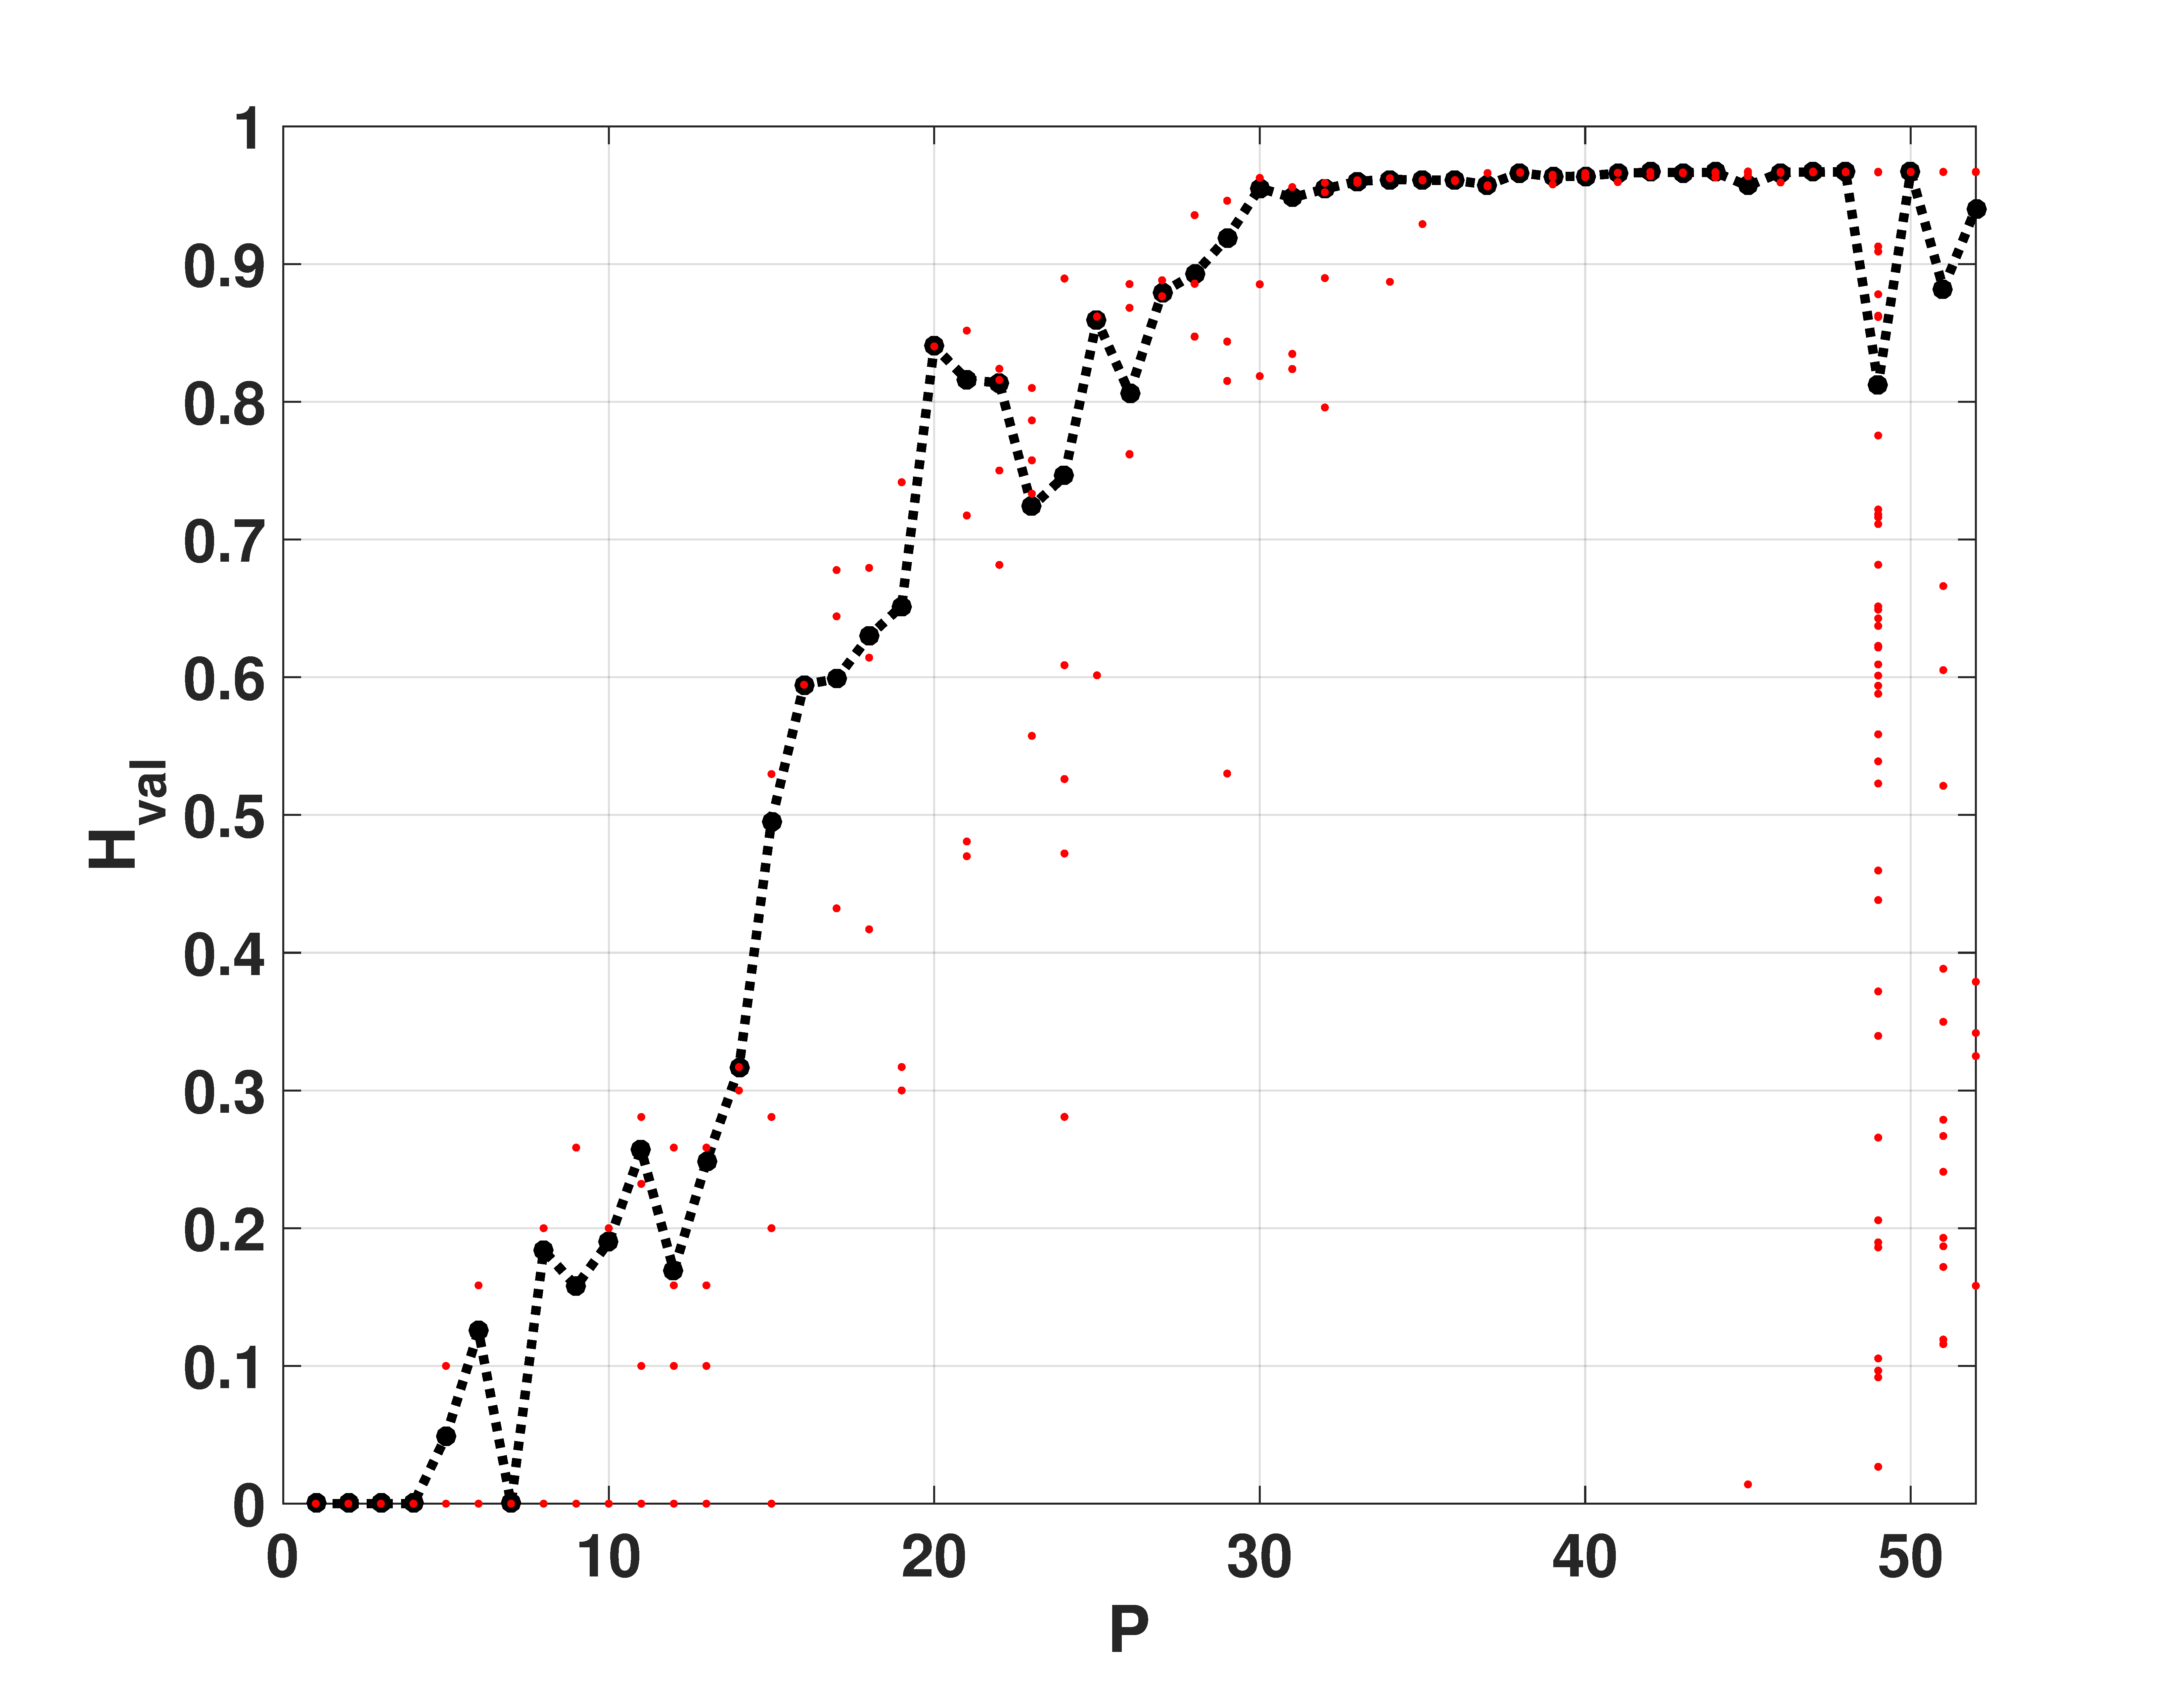
\includegraphics[width=.32\textwidth]{Hval_LogisticoB2}
	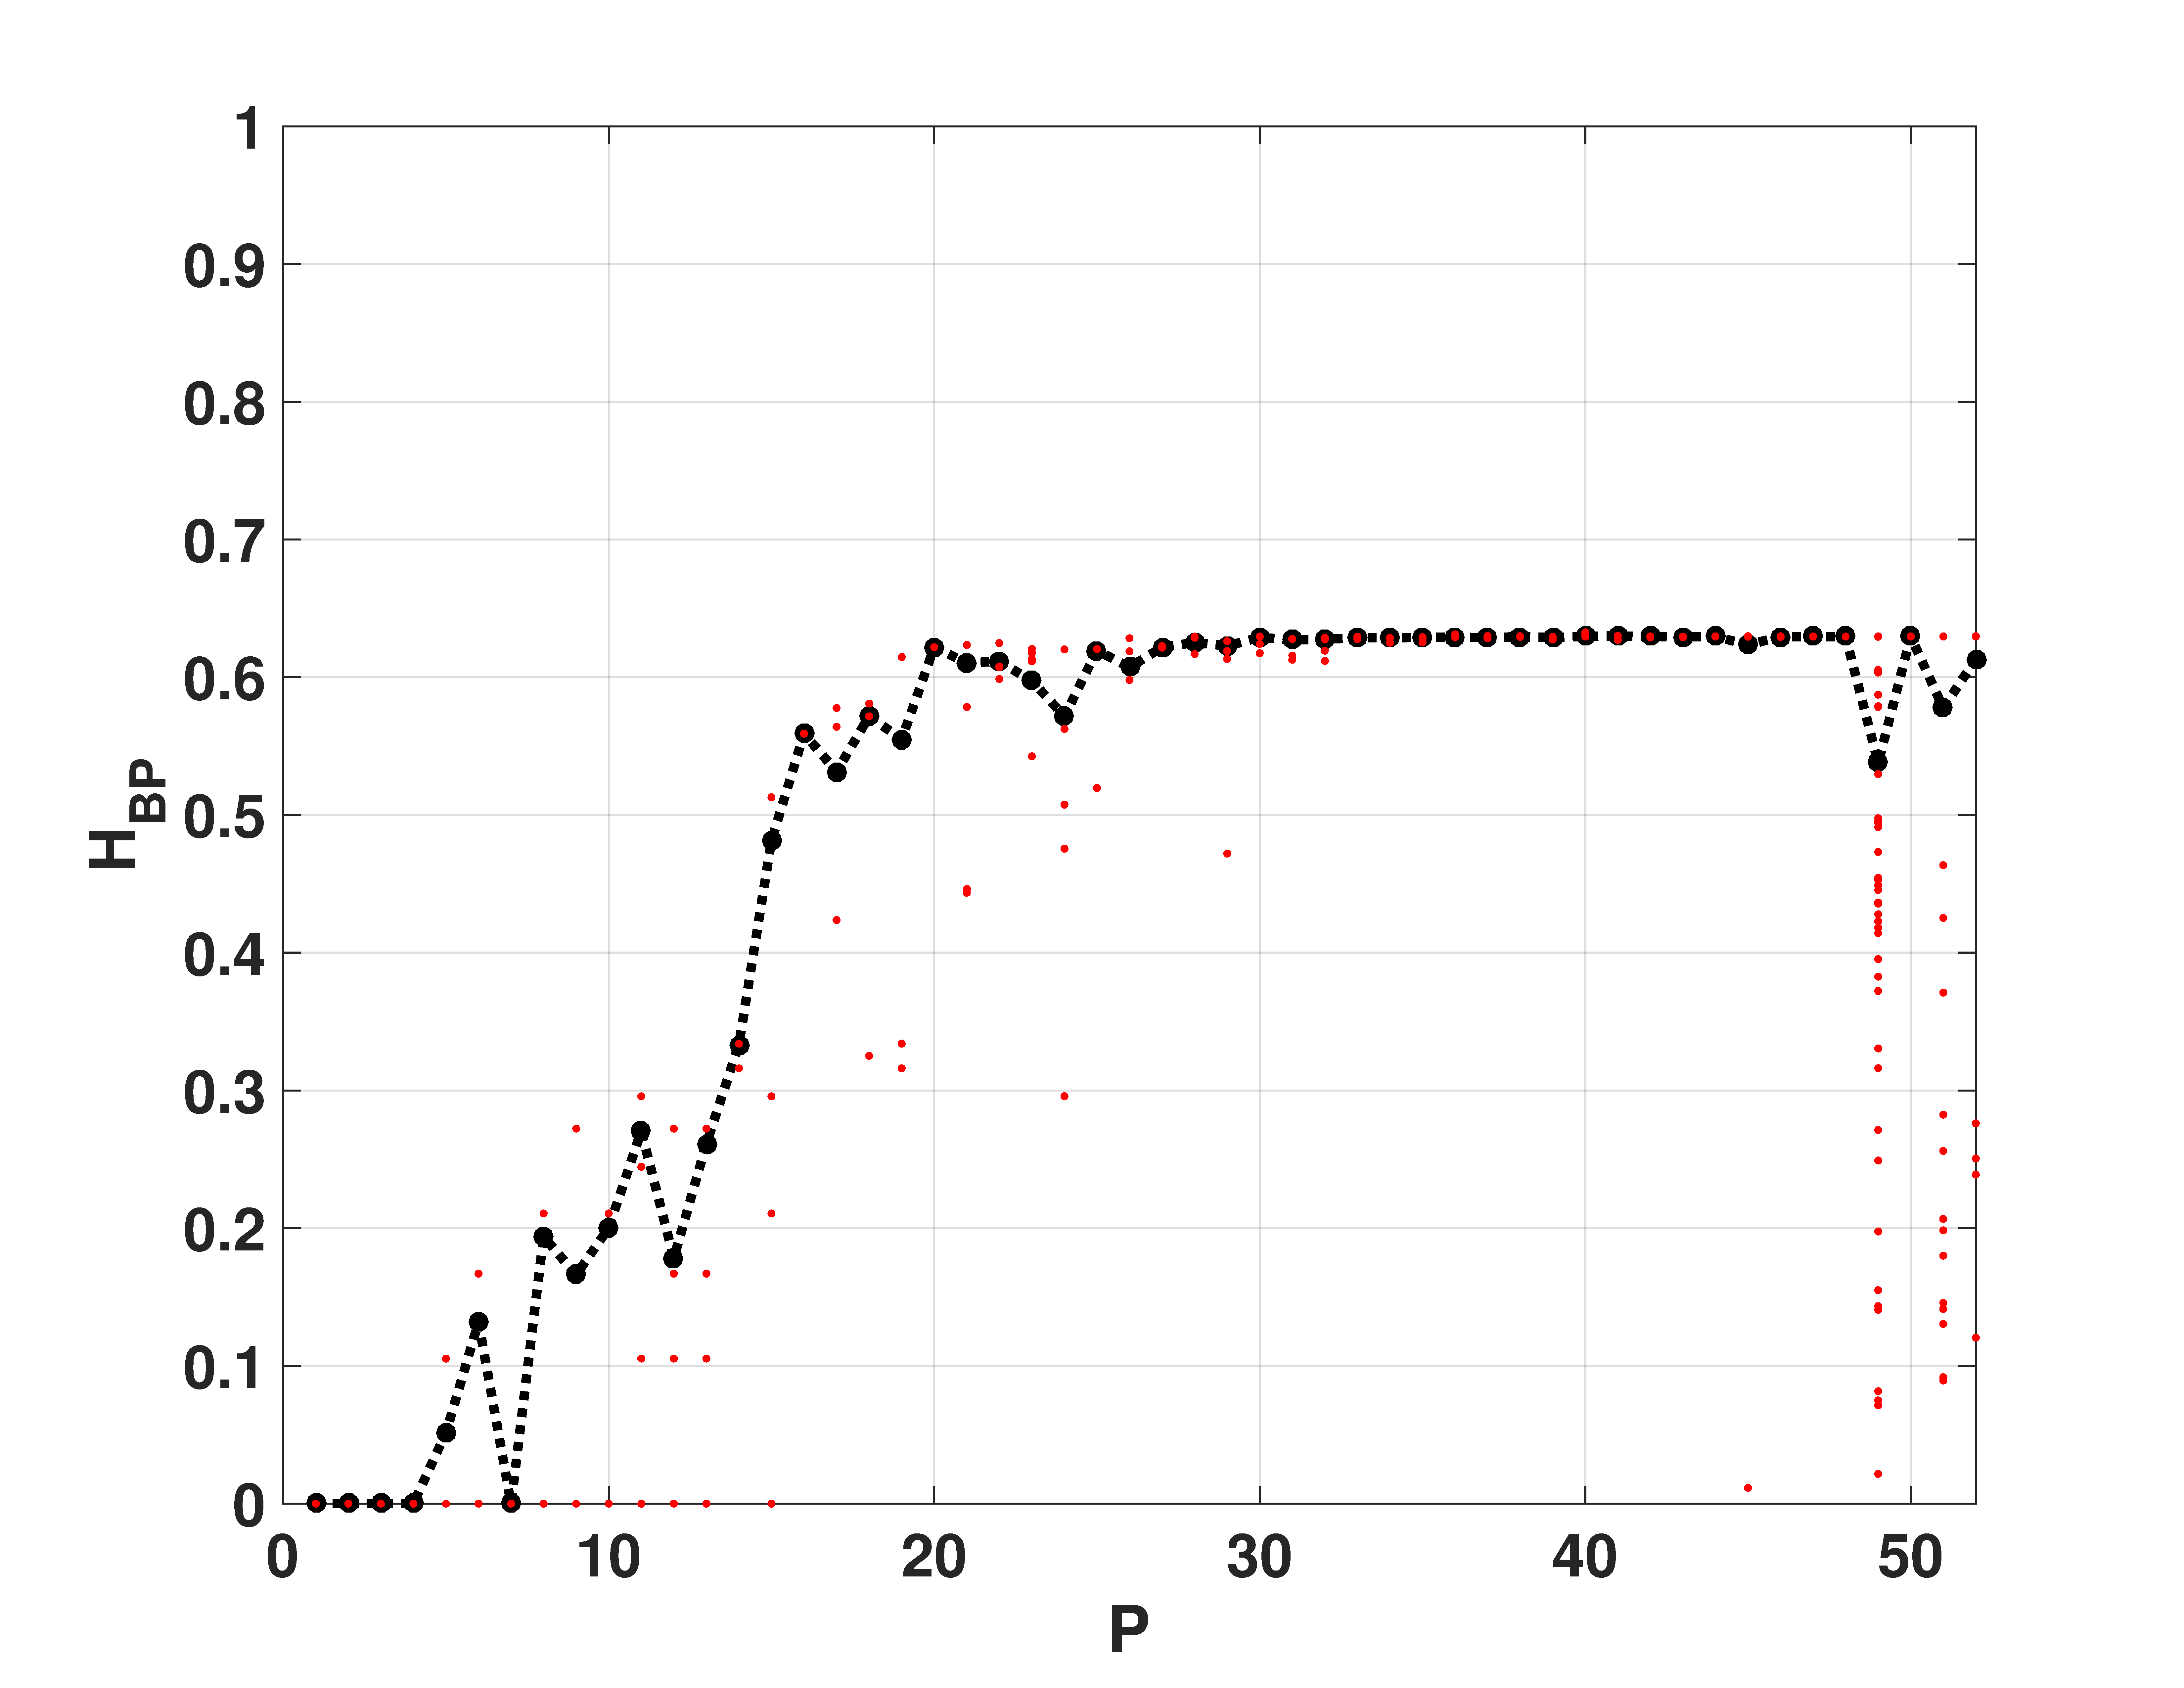
\includegraphics[width=.32\textwidth]{Hbp_LogisticoB2}
	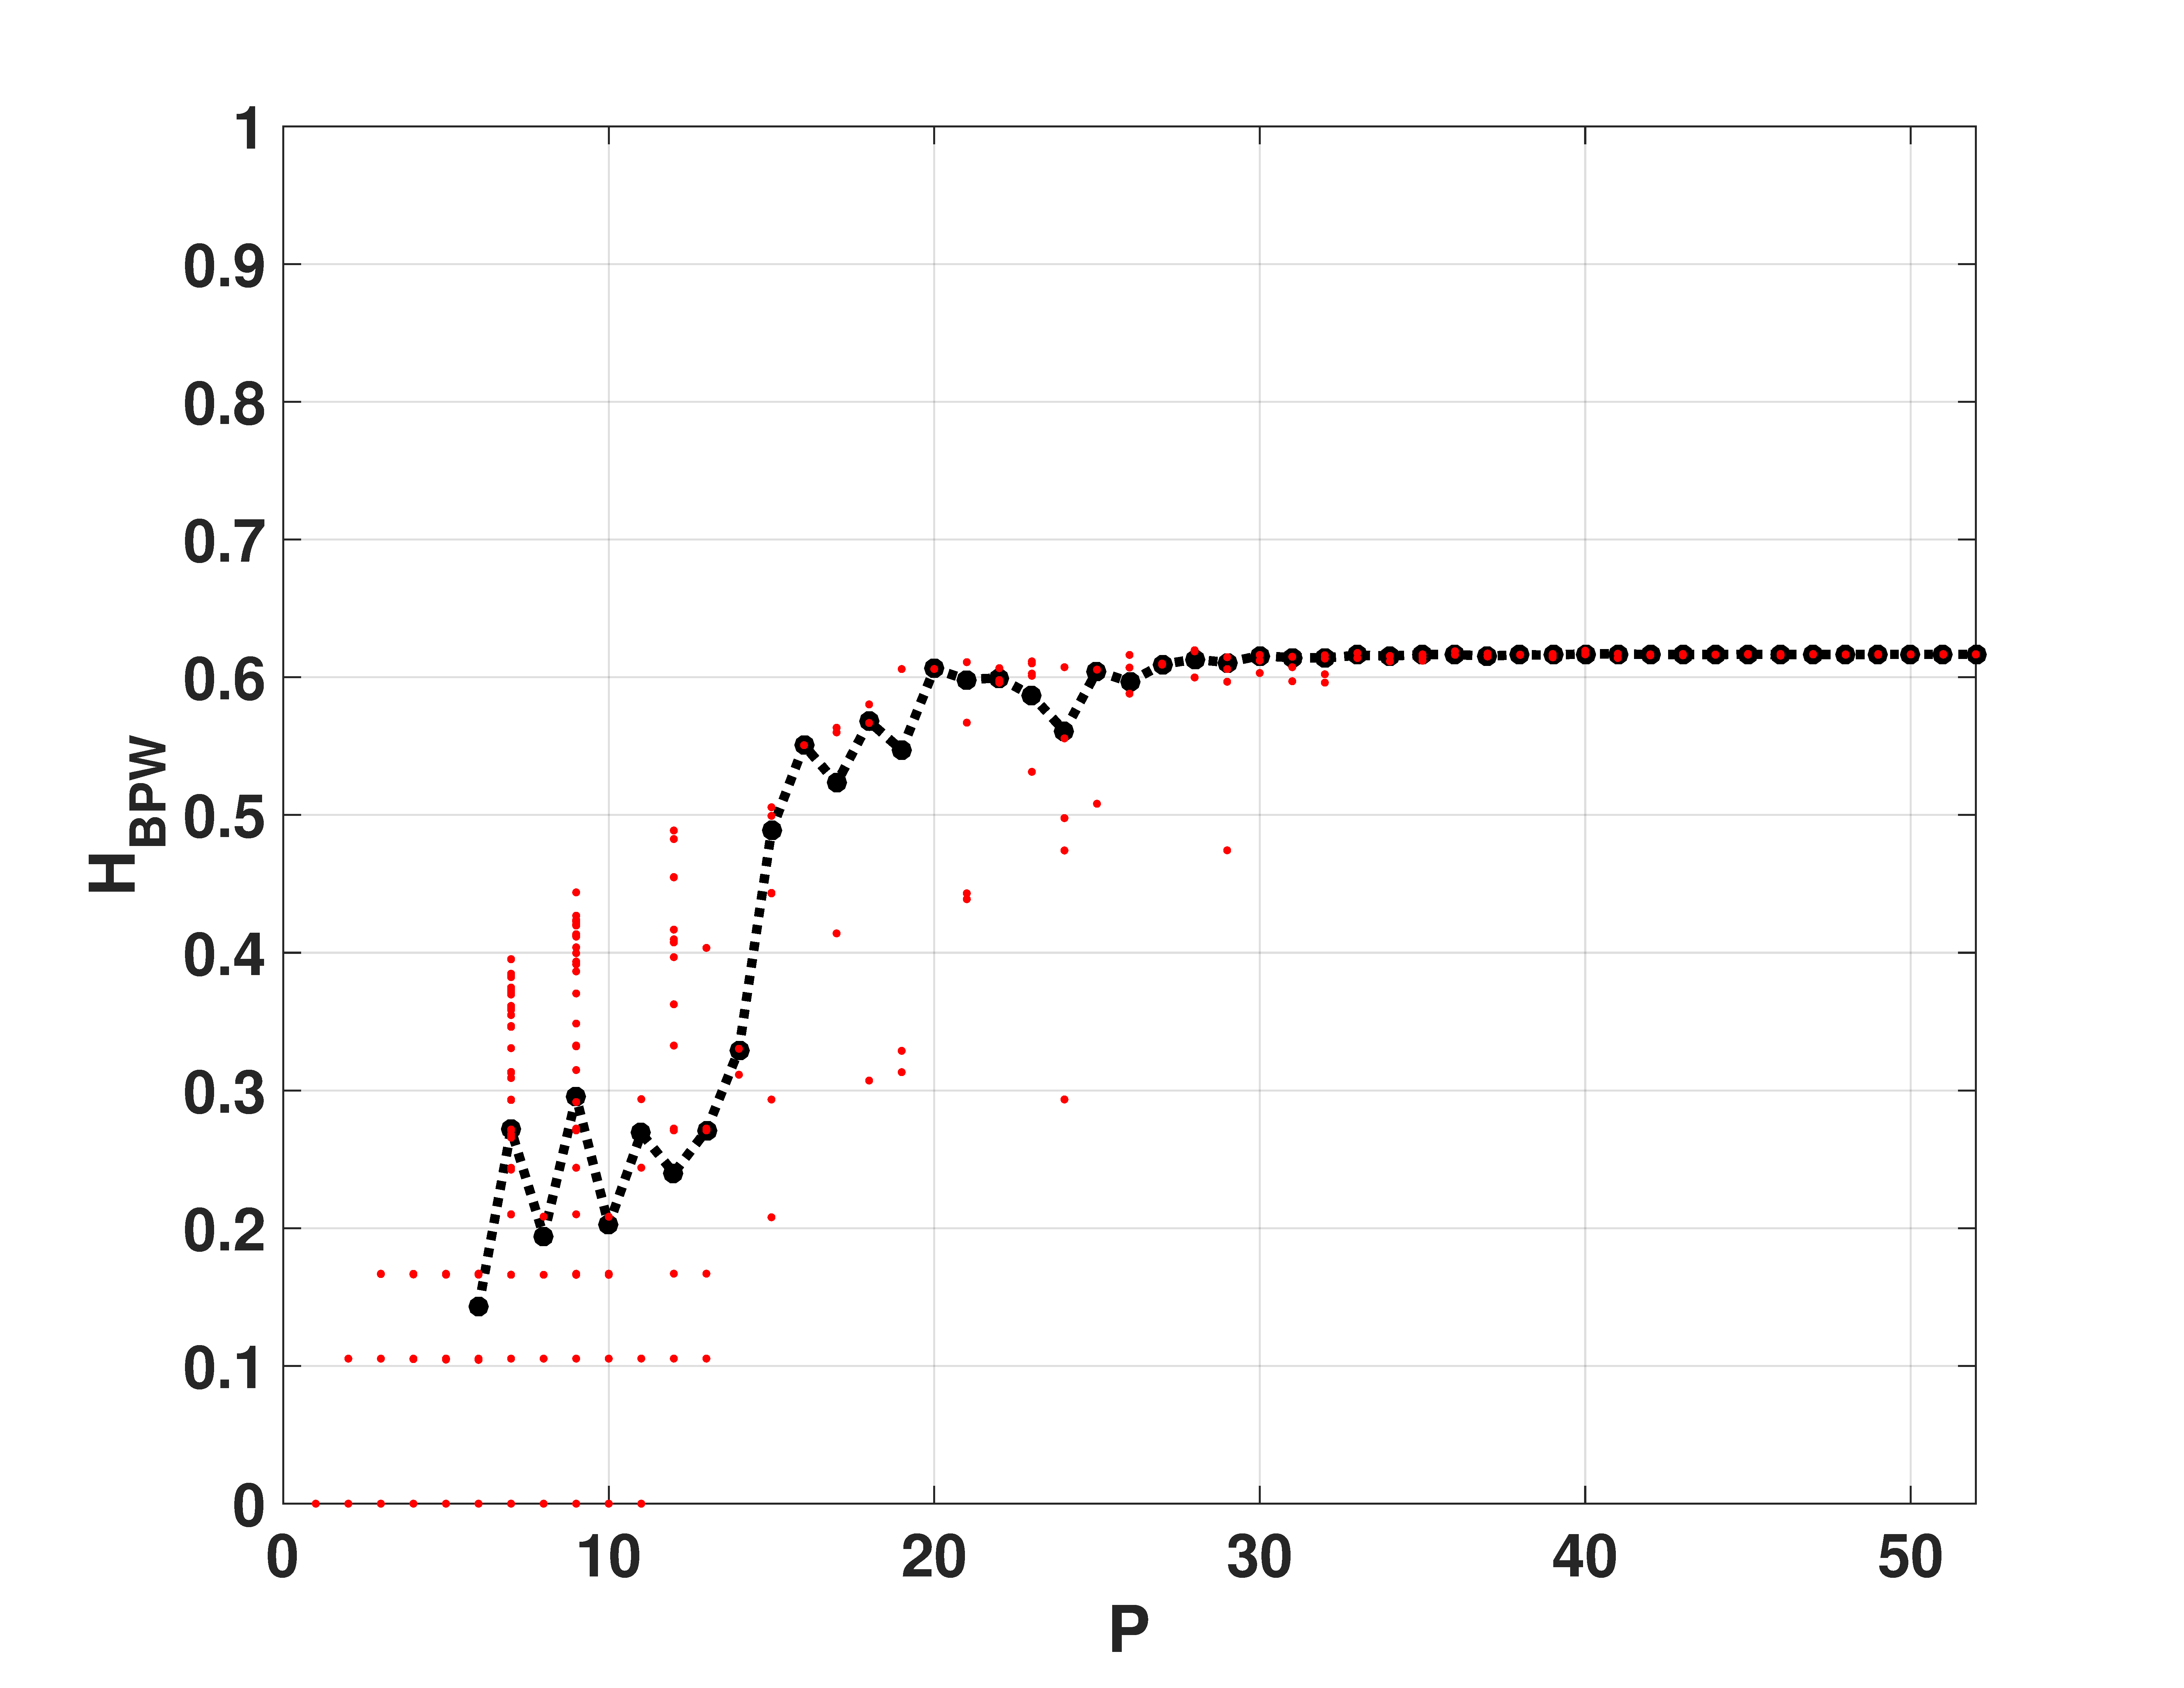
\includegraphics[width=.32\textwidth]{Hbpw_LogisticoB2}
	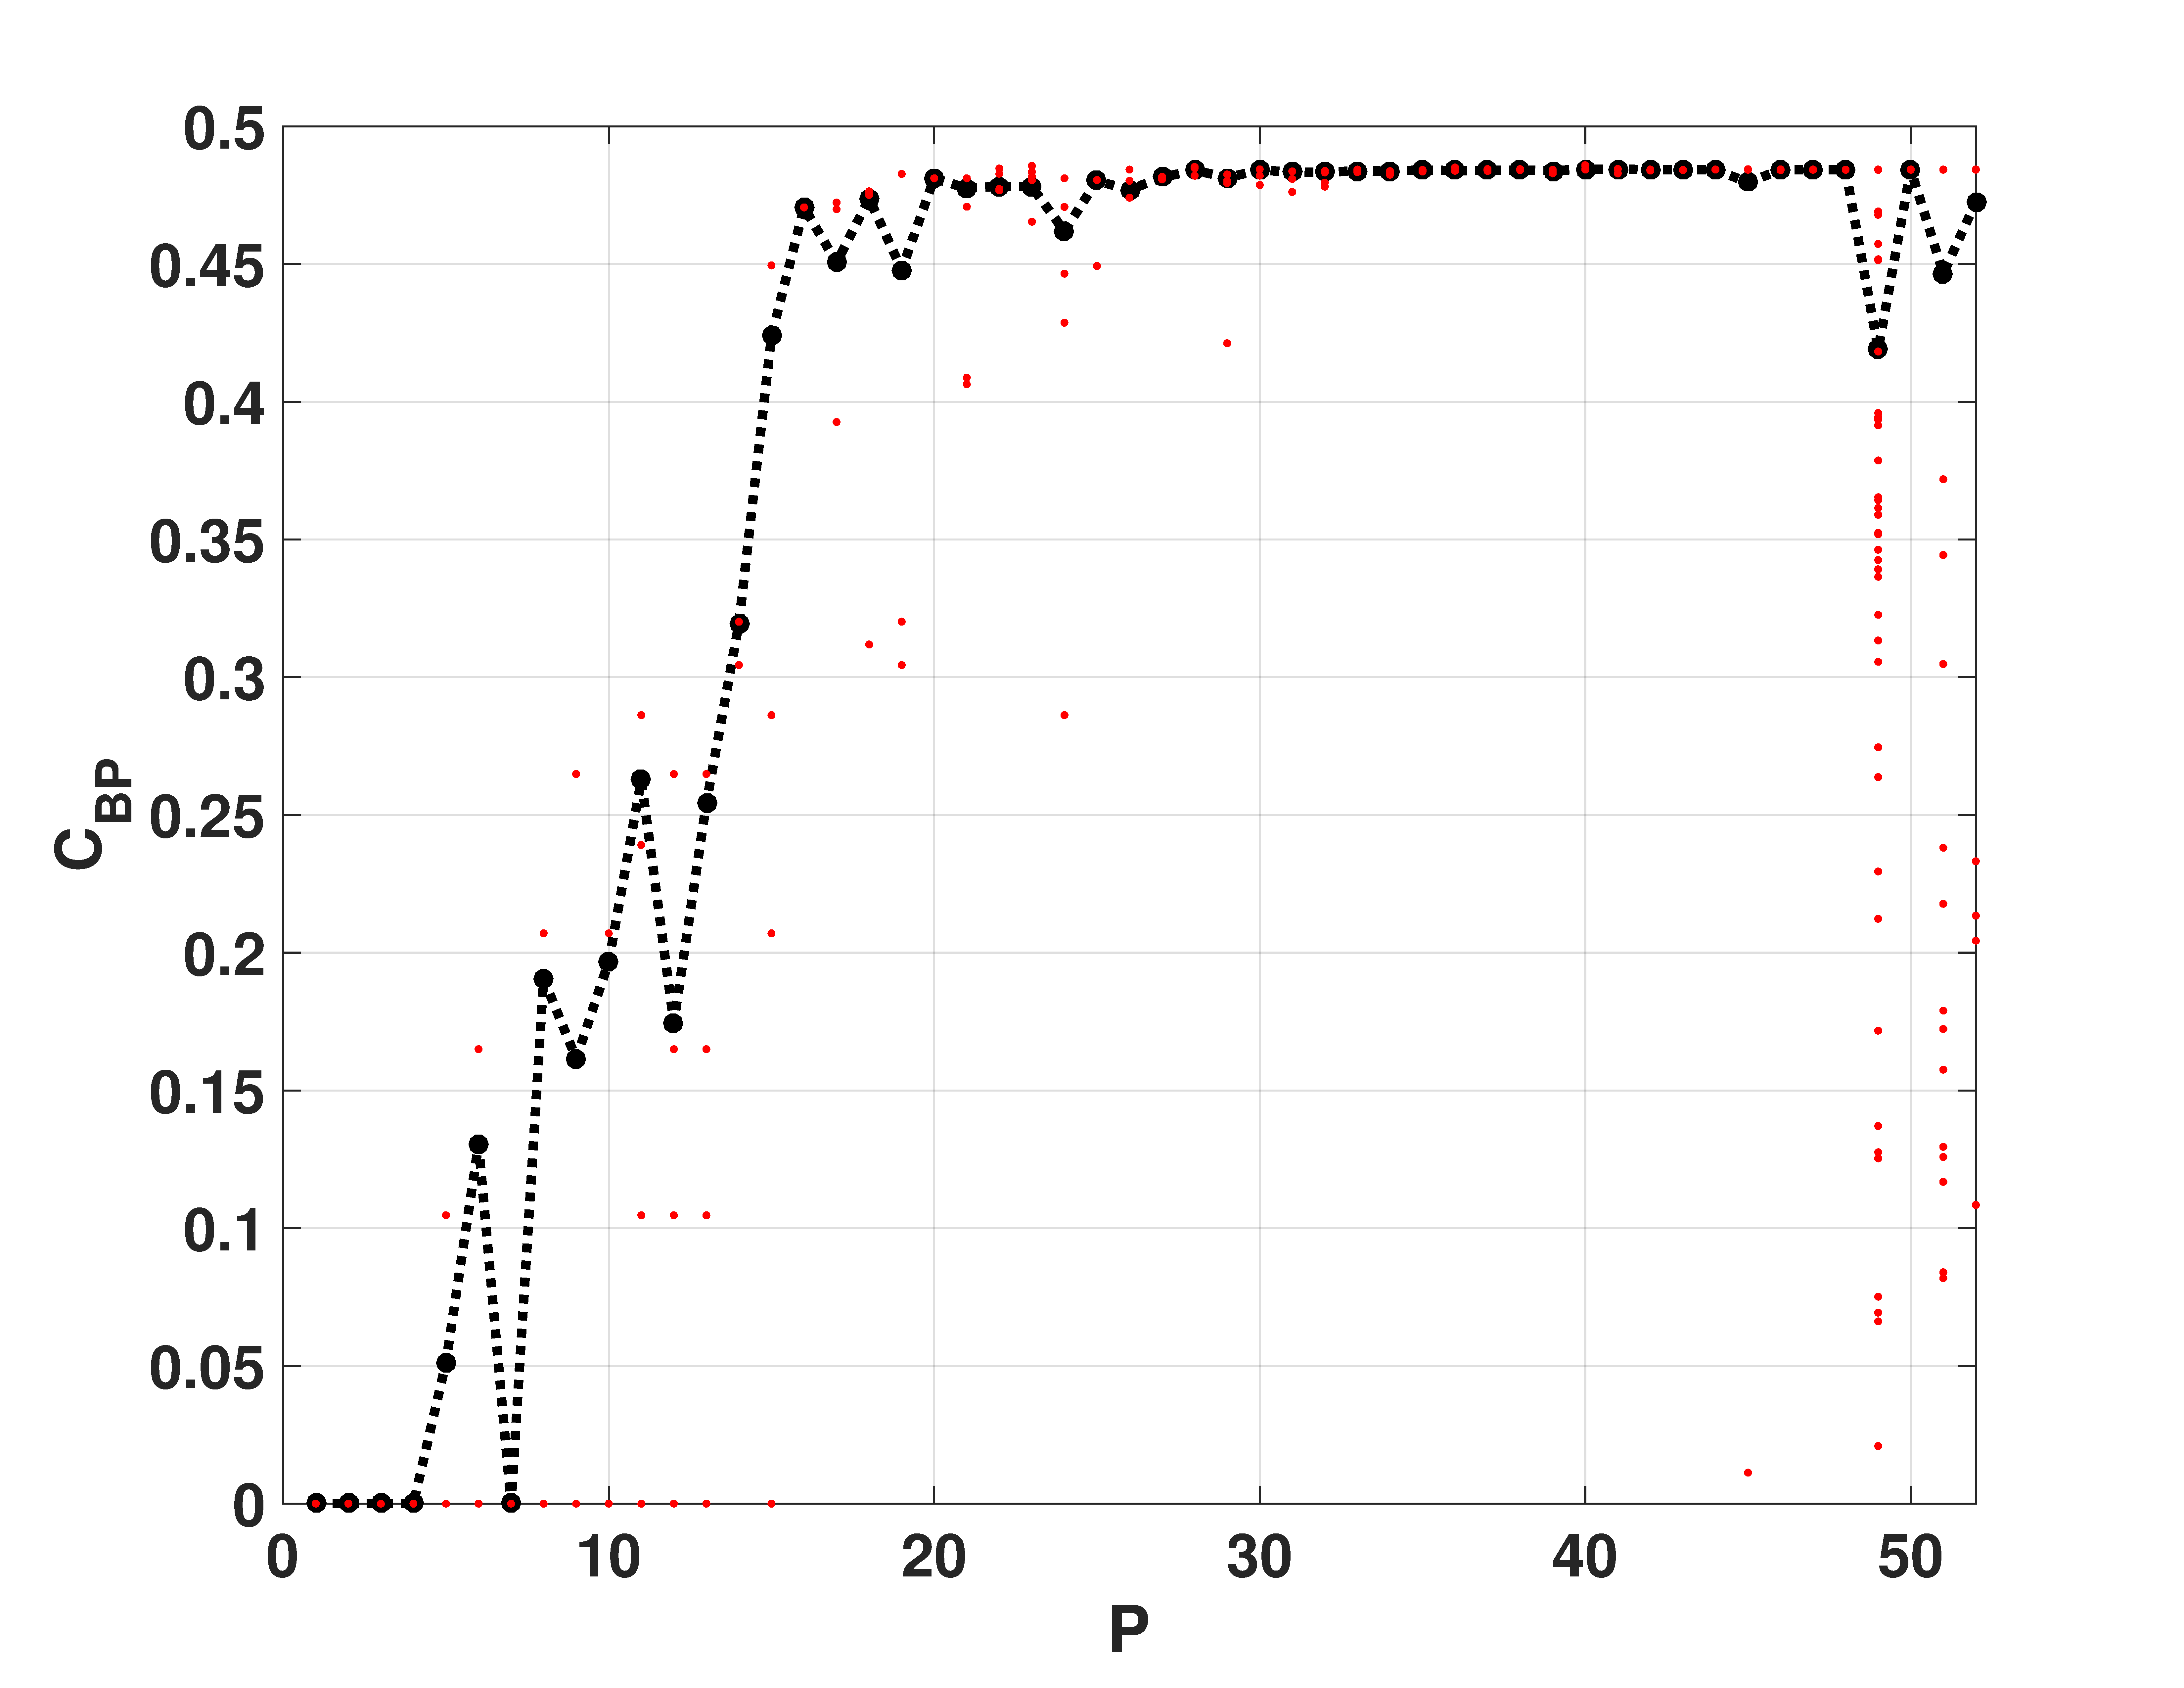
\includegraphics[width=.32\textwidth]{Cbp_LogisticoB2}
	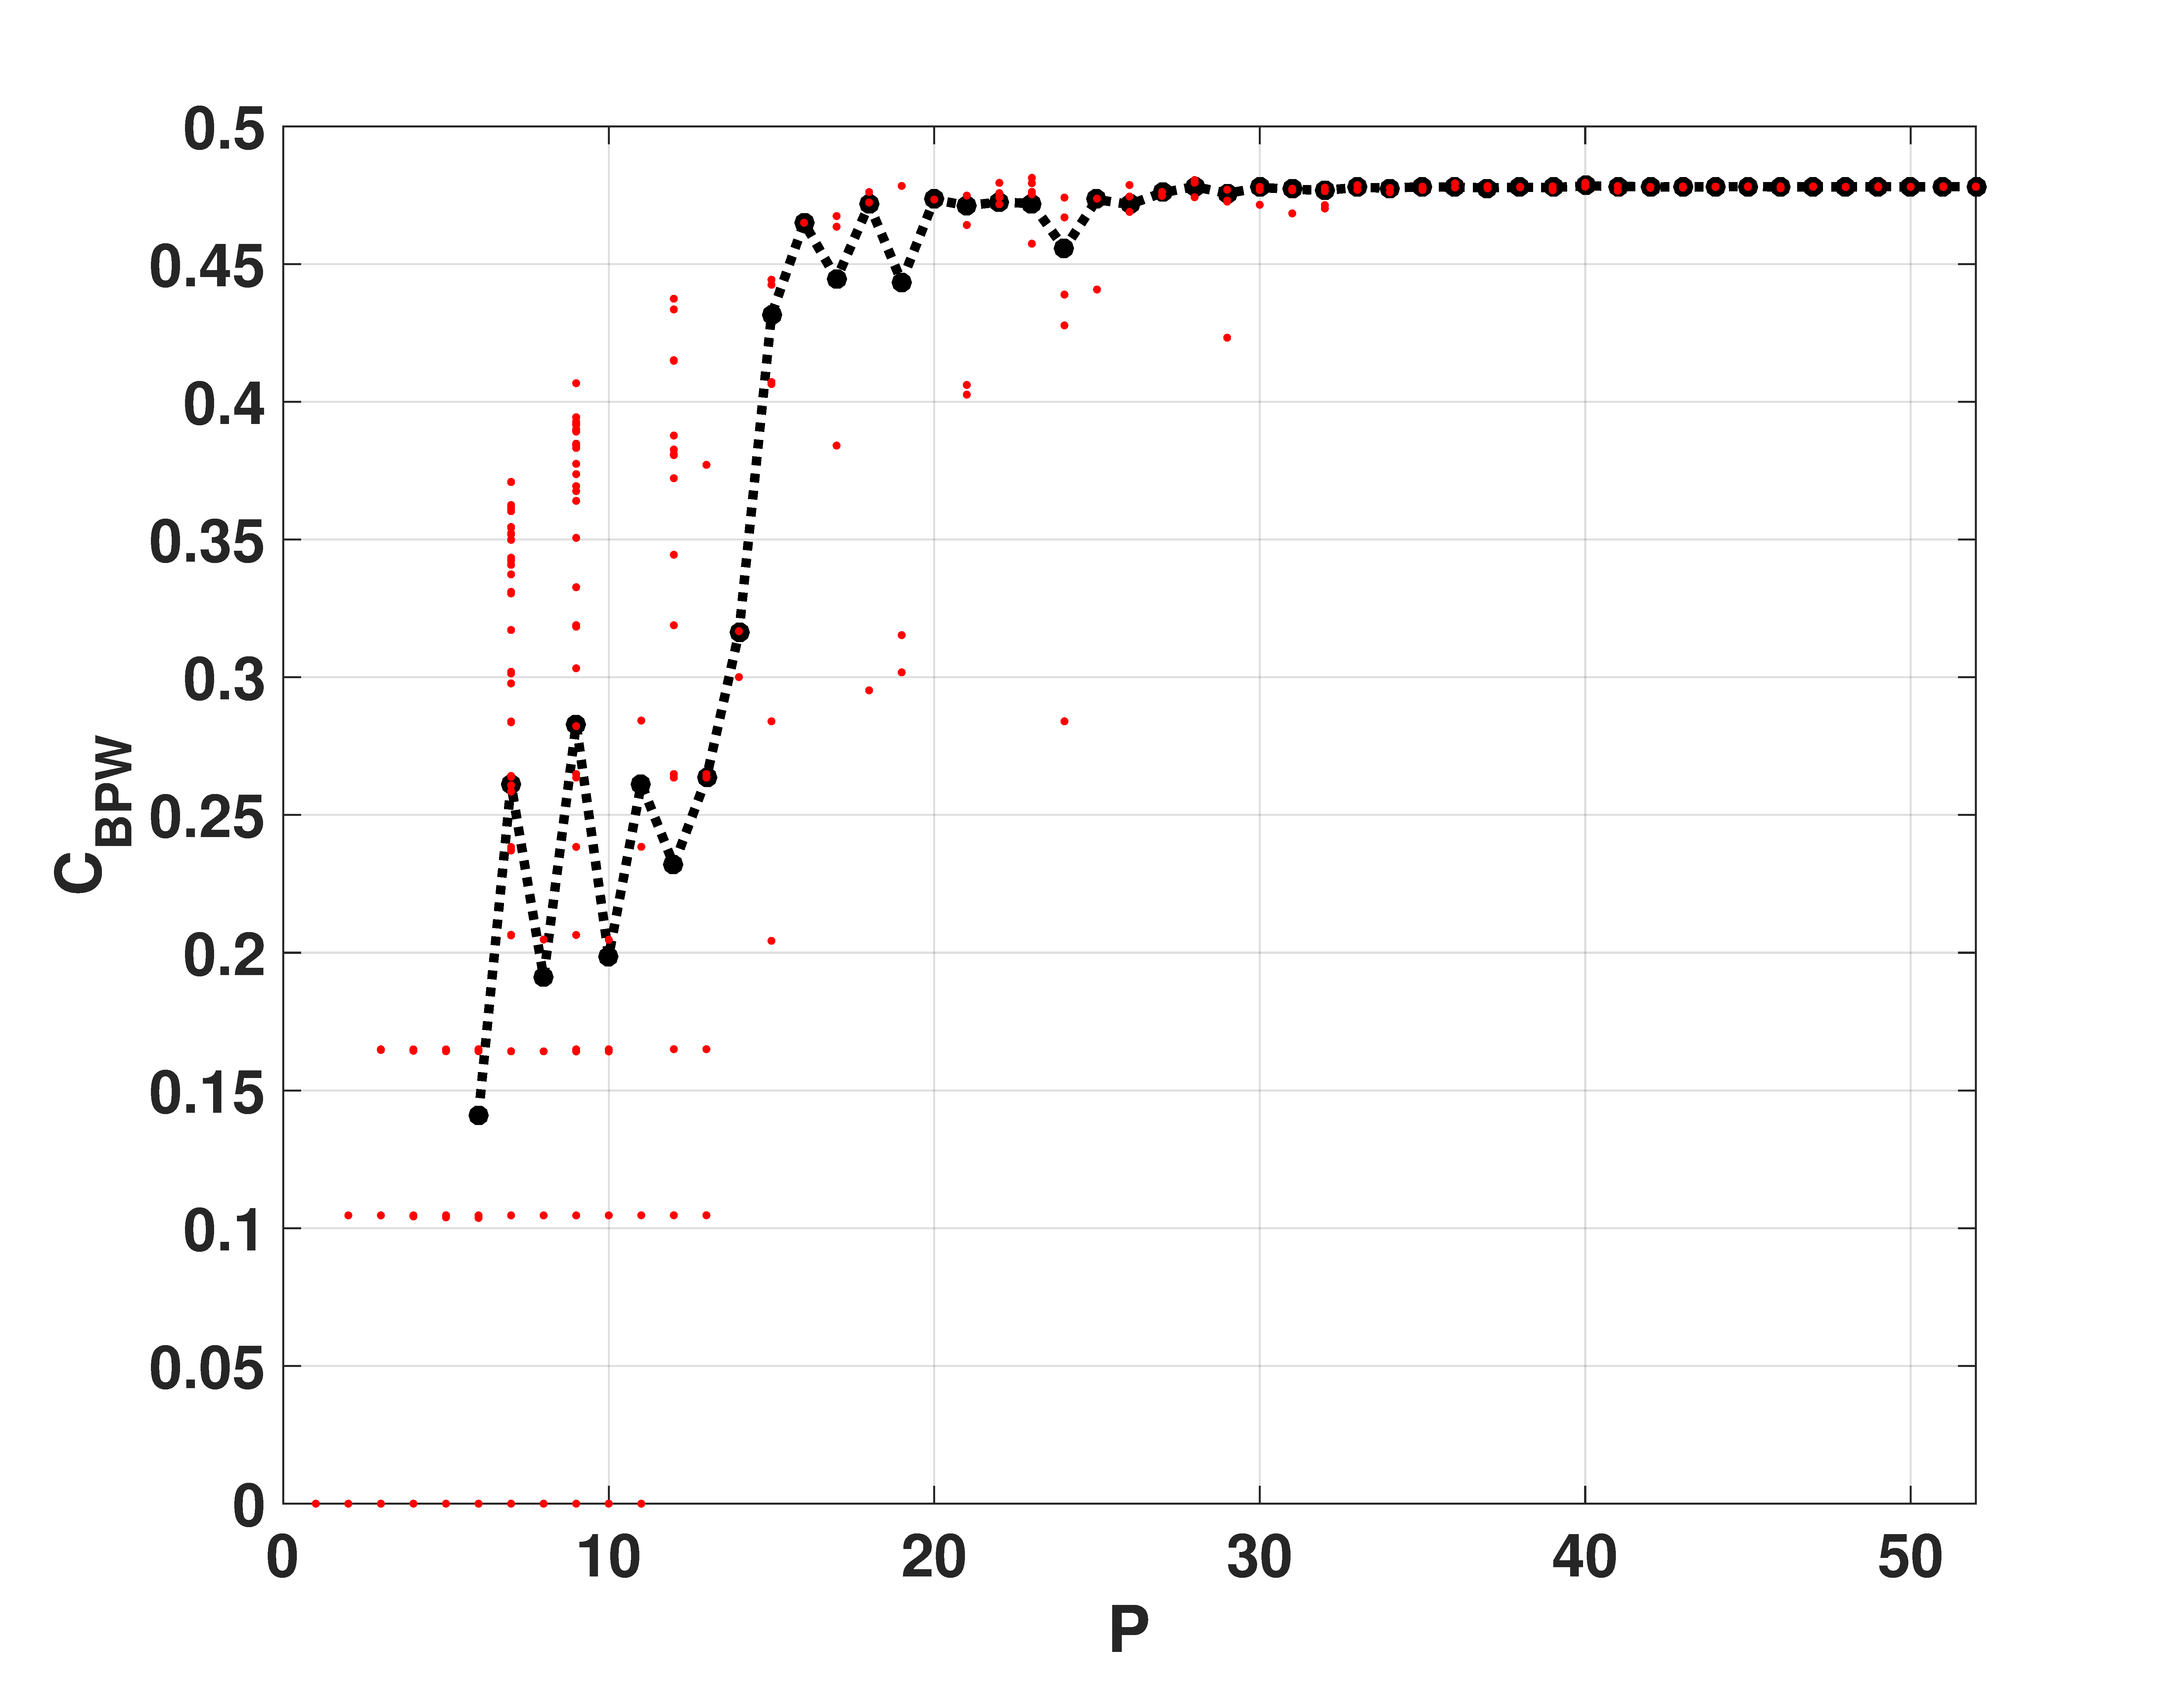
\includegraphics[width=.32\textwidth]{Cbpw_LogisticoB2}
	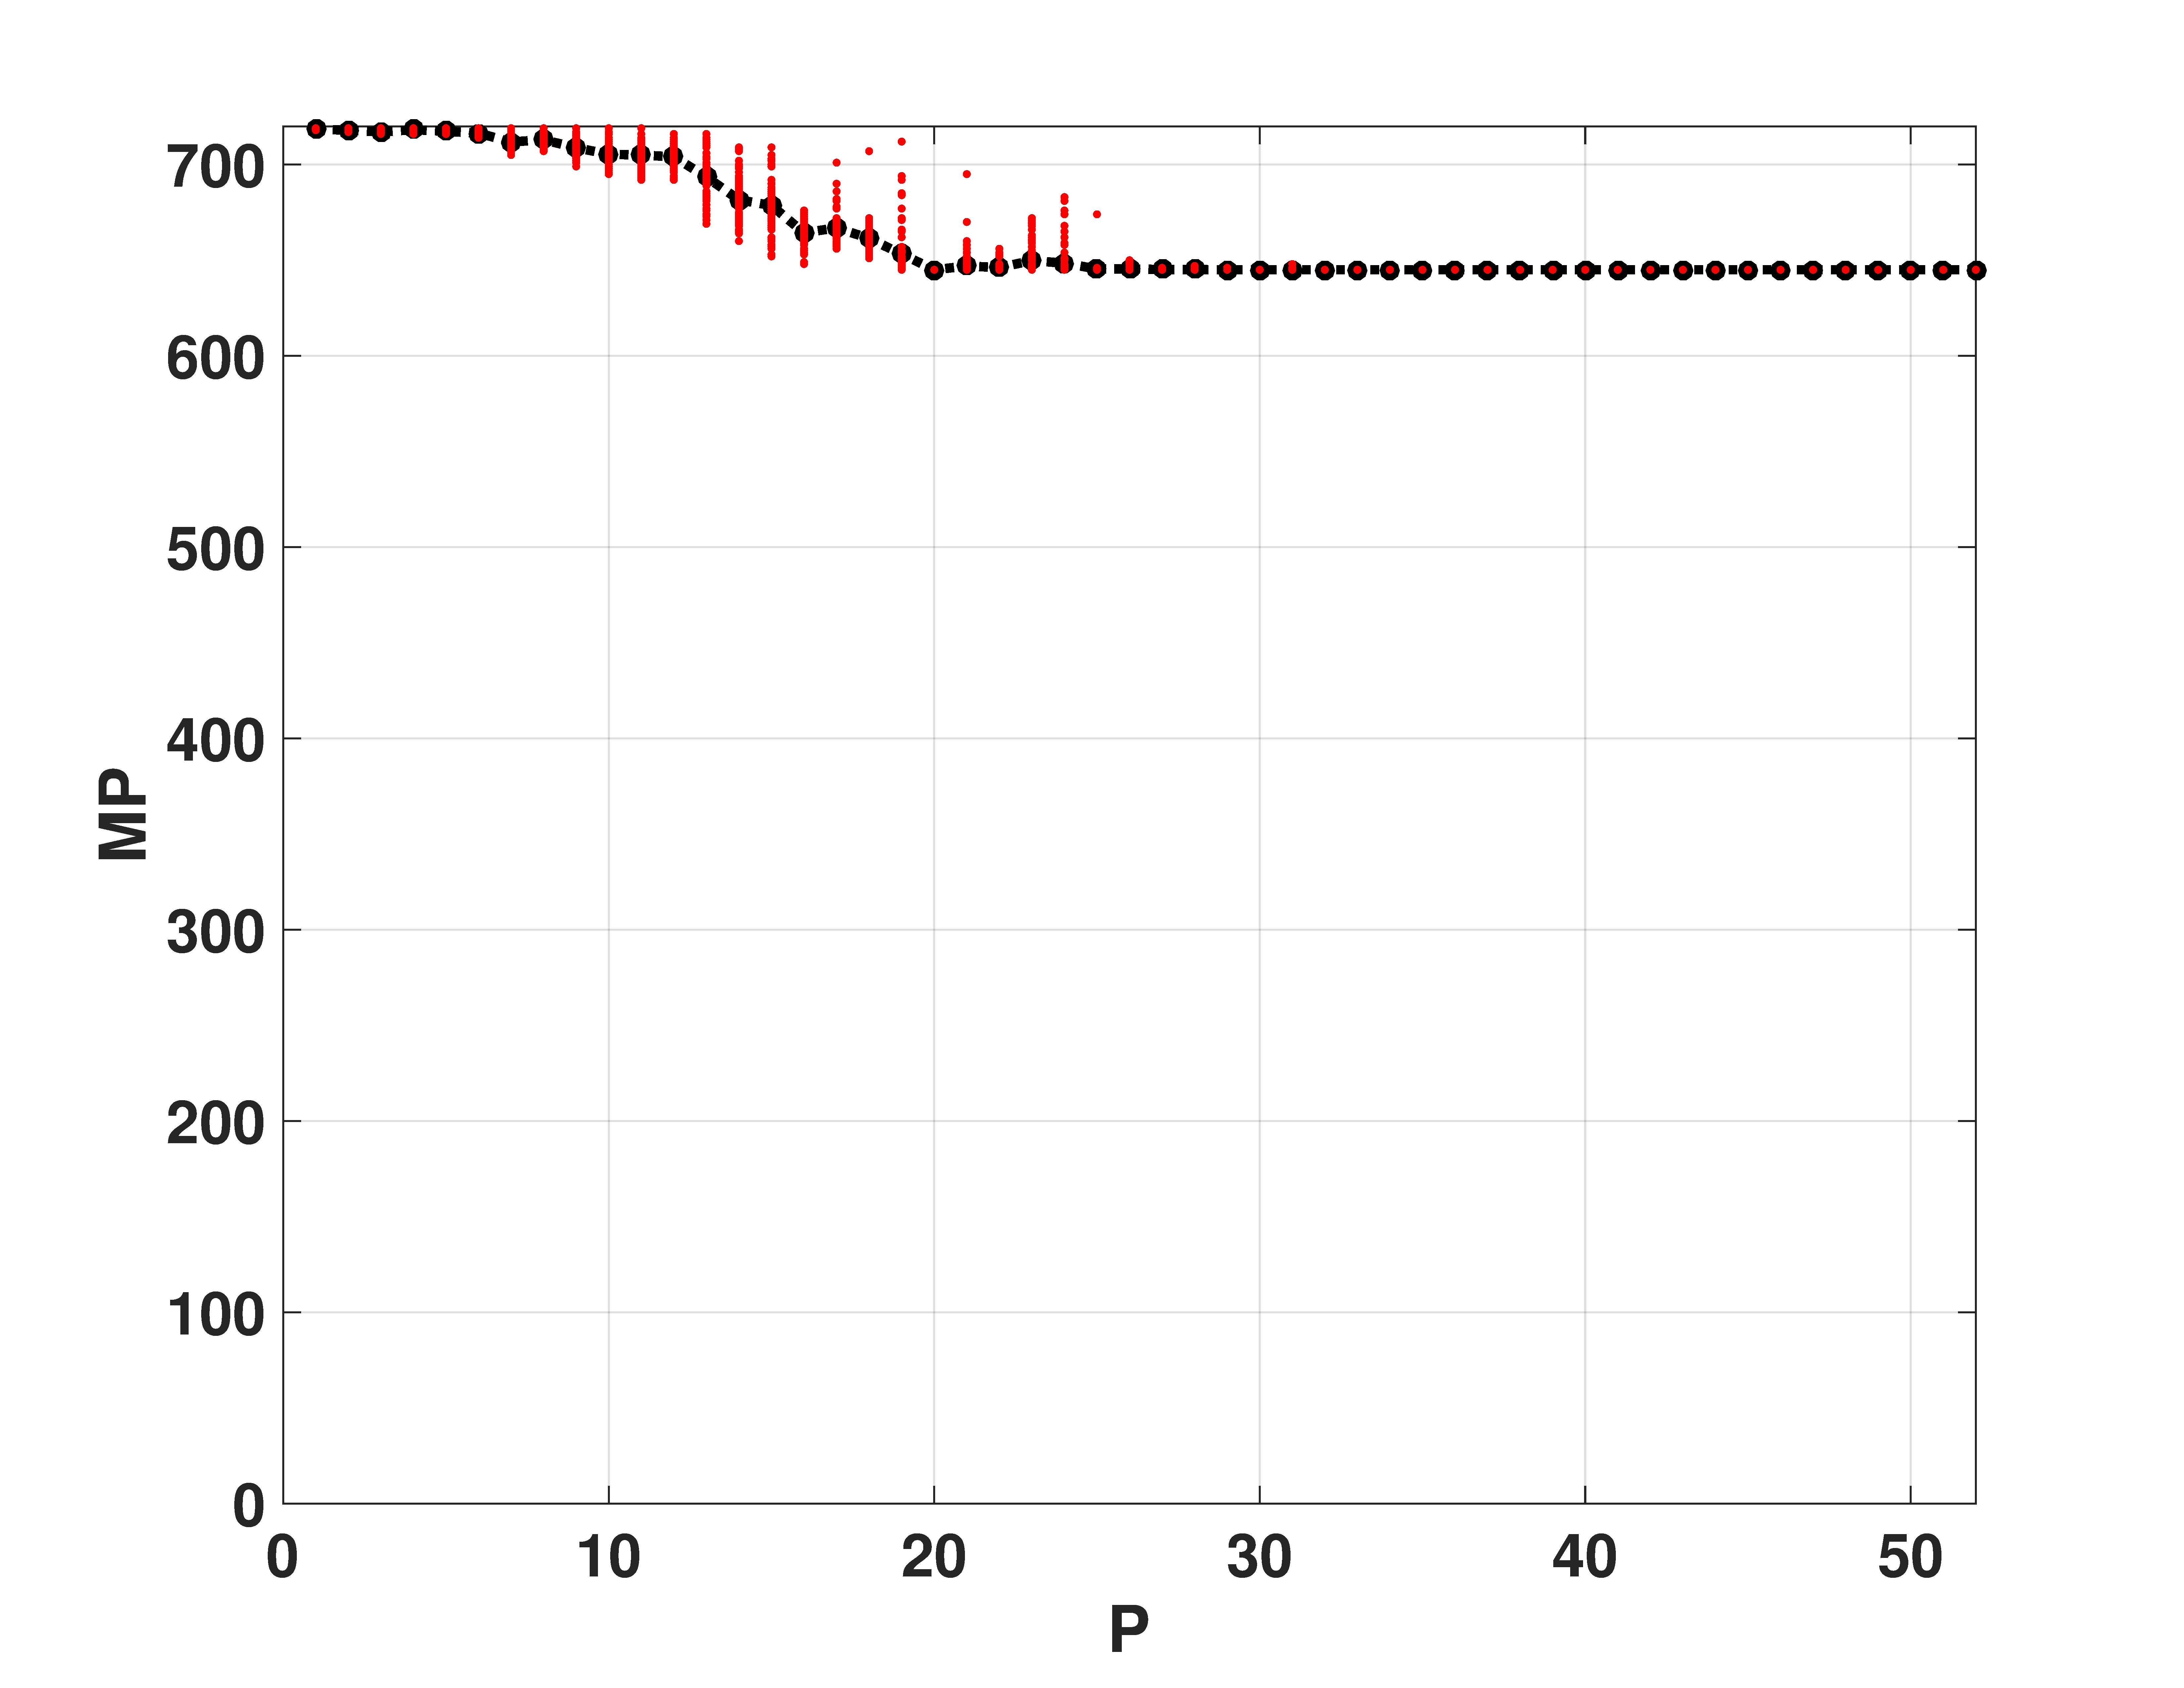
\includegraphics[width=.32\textwidth]{MP_LogisticoB2}
	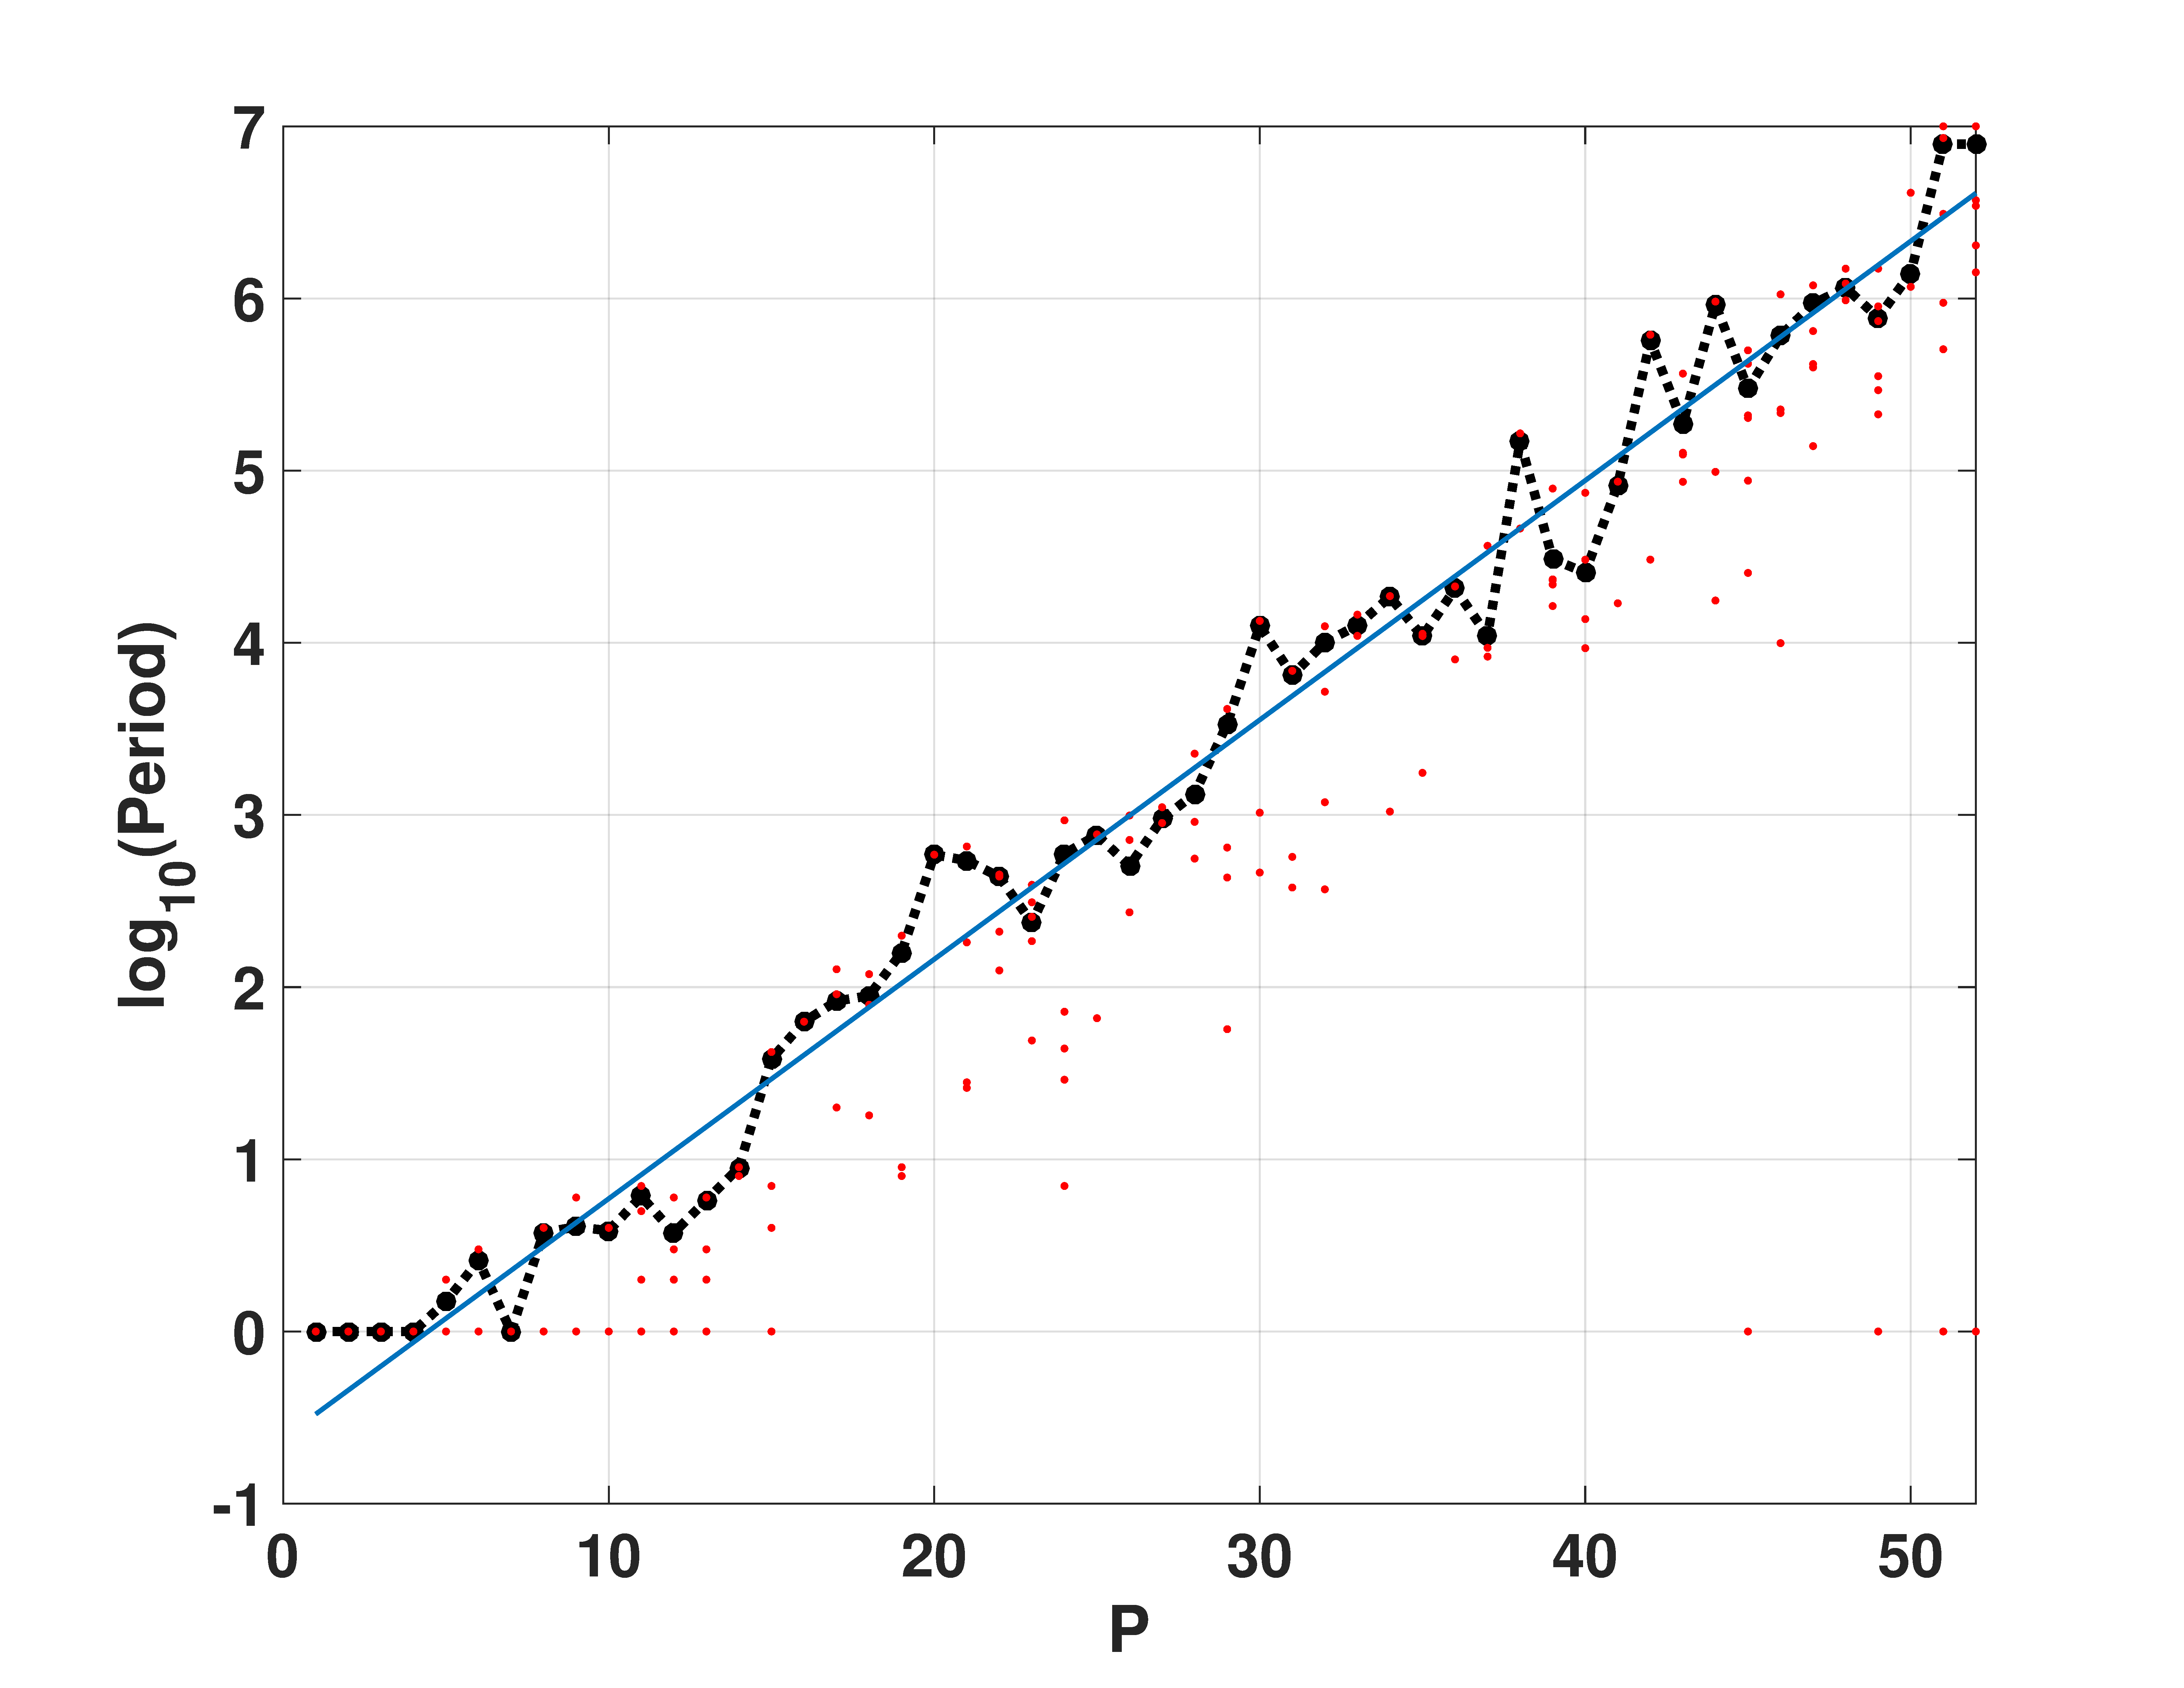
\includegraphics[width=.32\textwidth]{Period_LogisticoB2}
	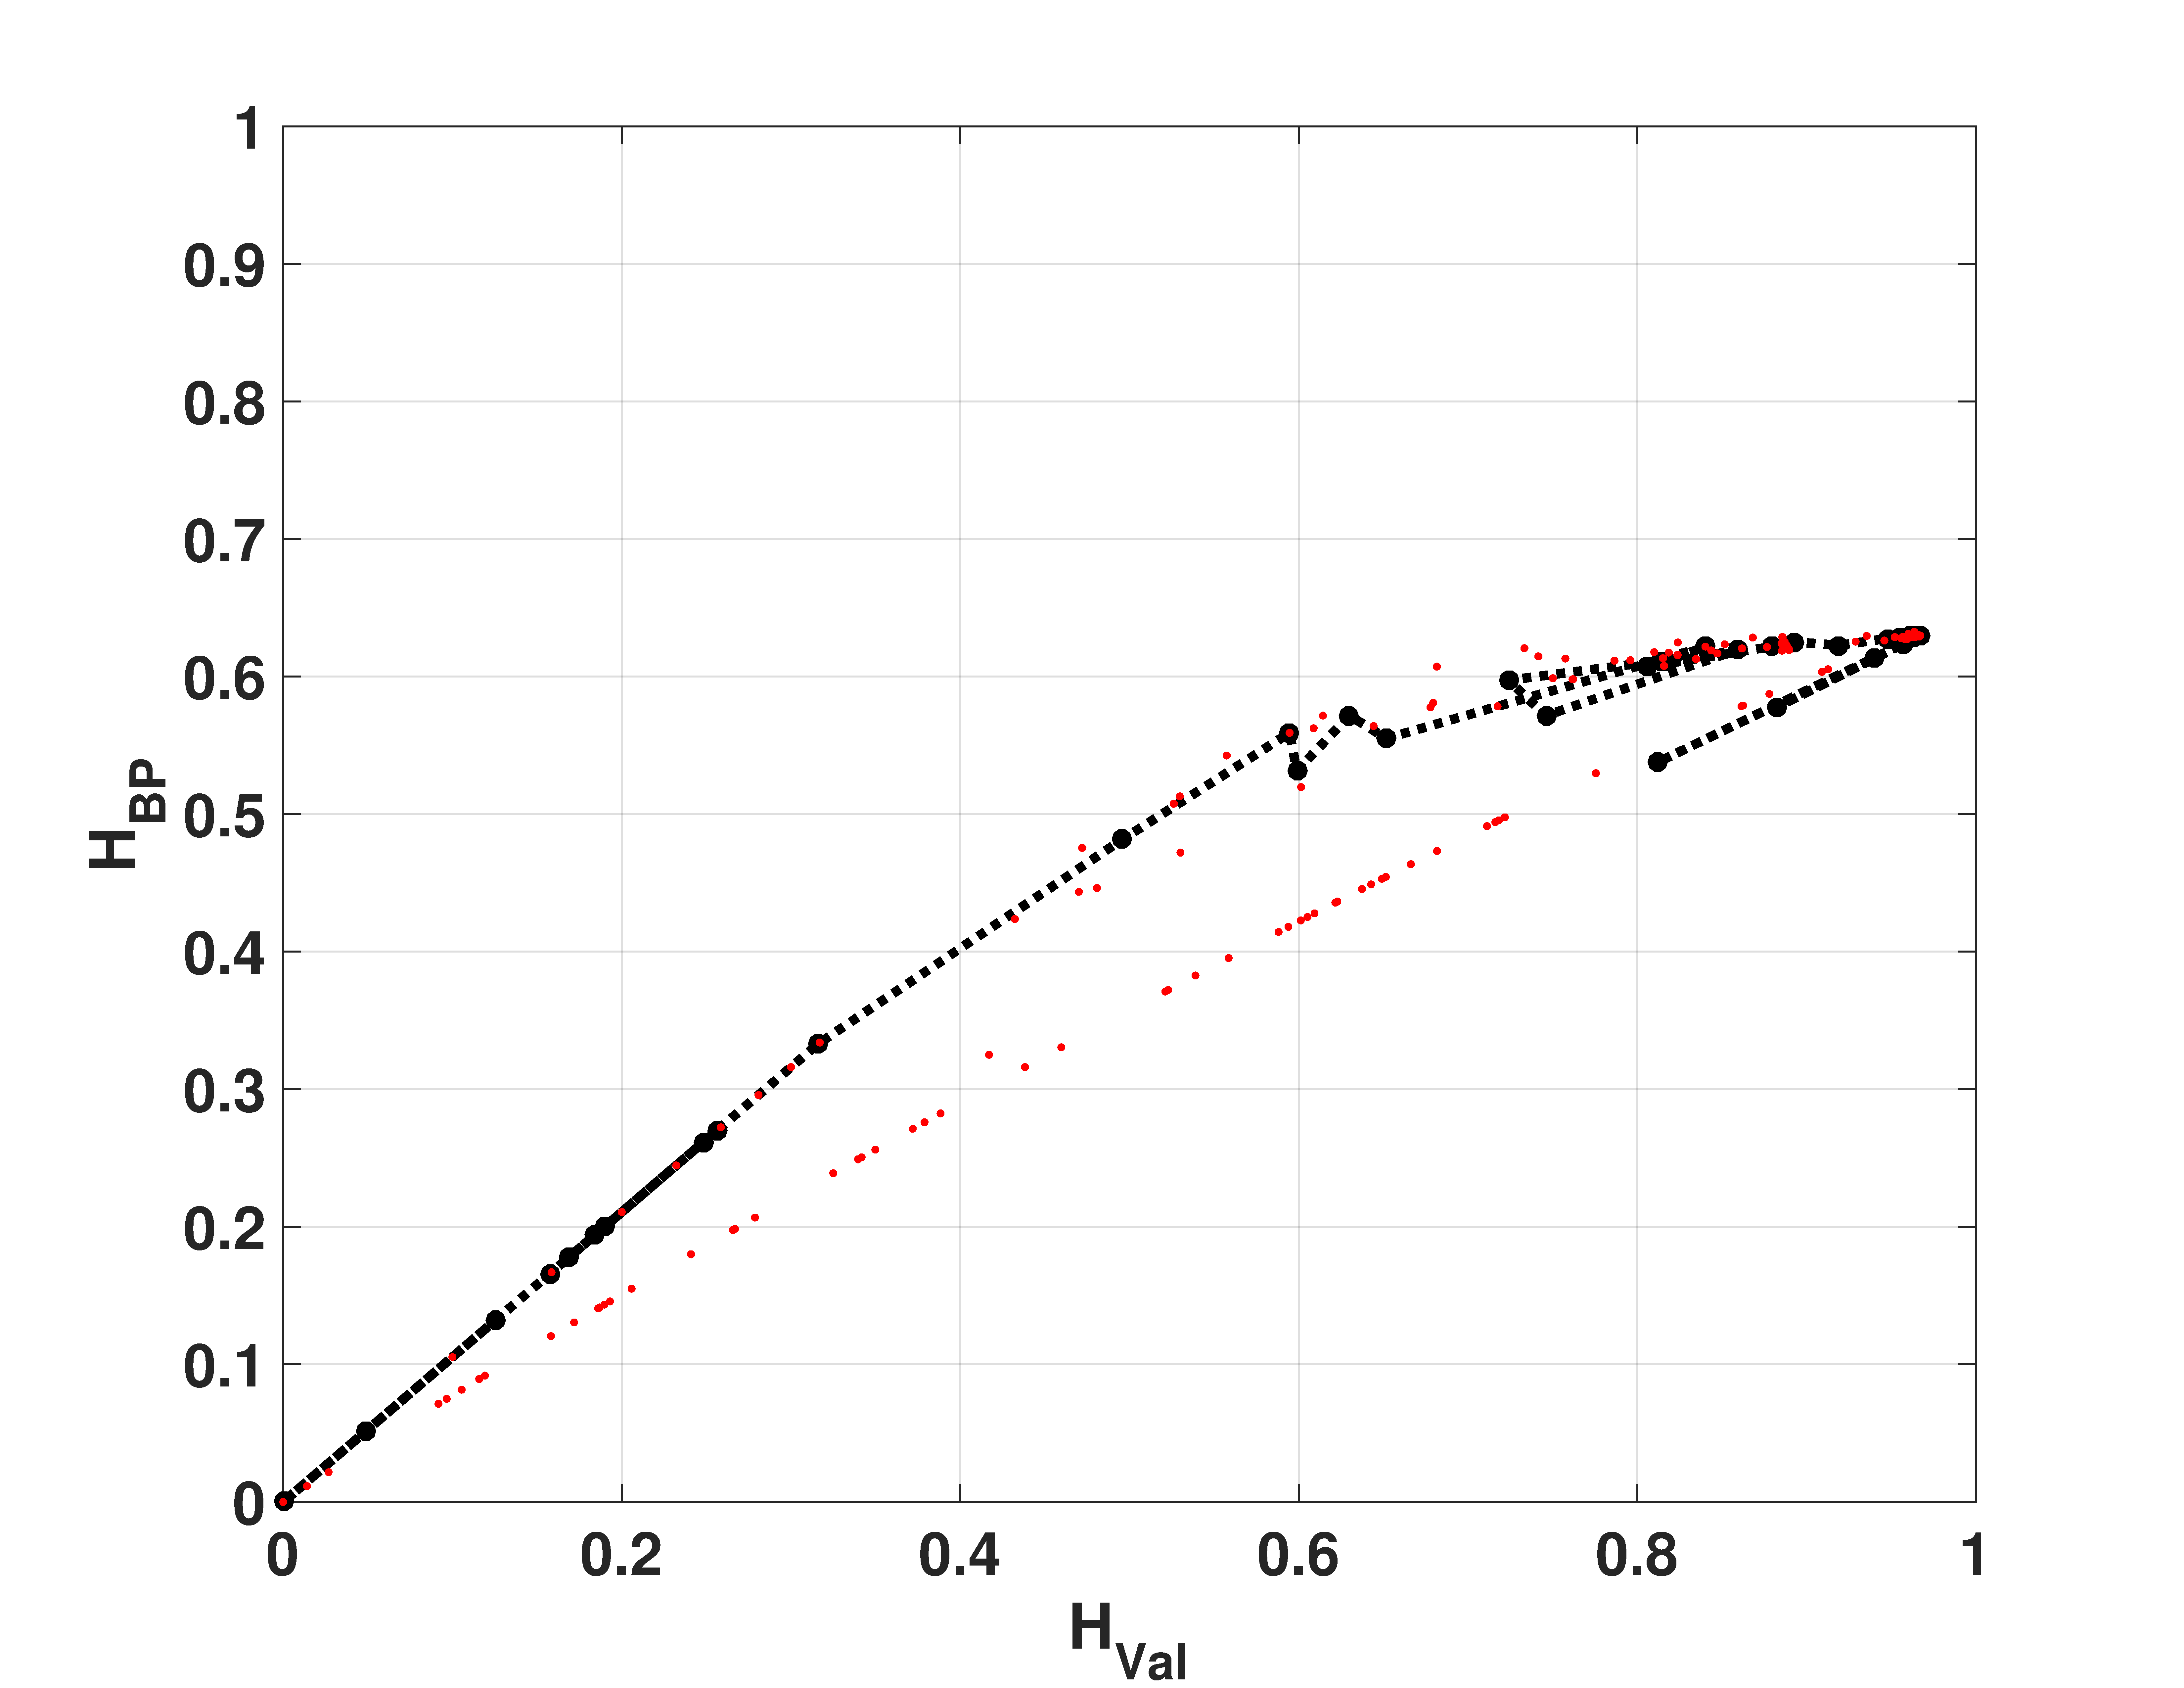
\includegraphics[width=.32\textwidth]{HbpHval_LogisticoB2}
	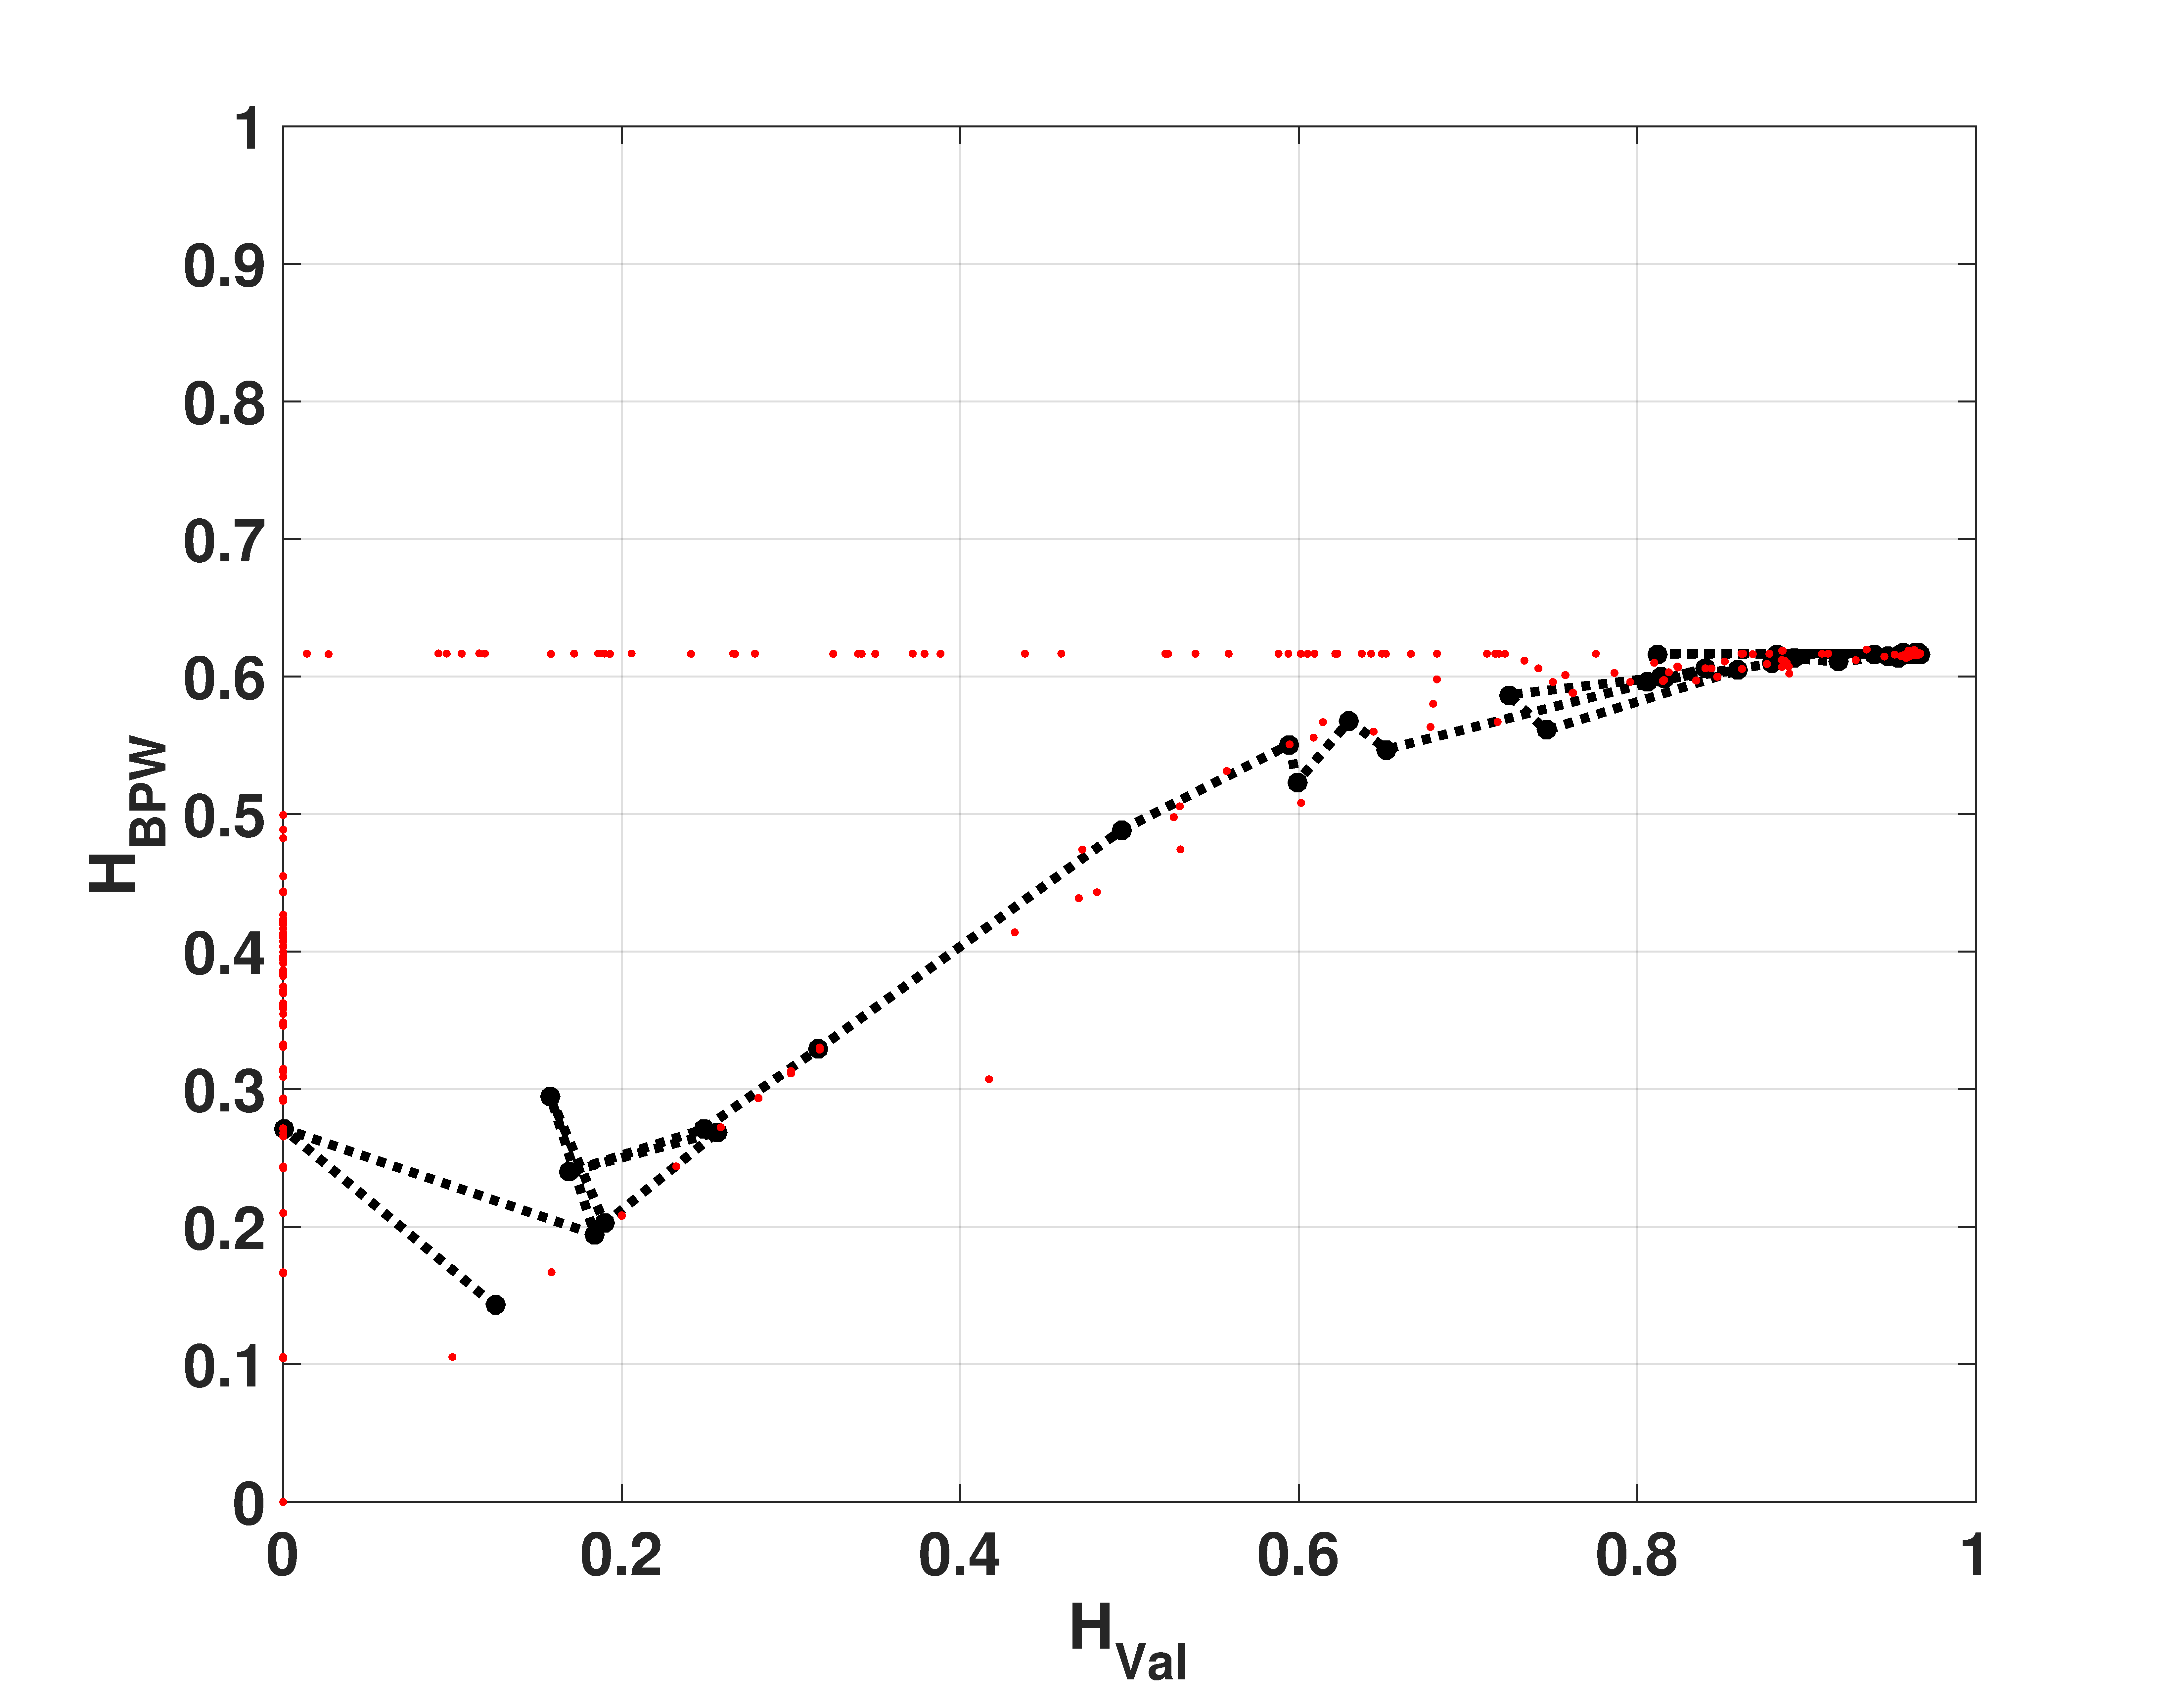
\includegraphics[width=.32\textwidth]{HbpwHval_LogisticoB2}
	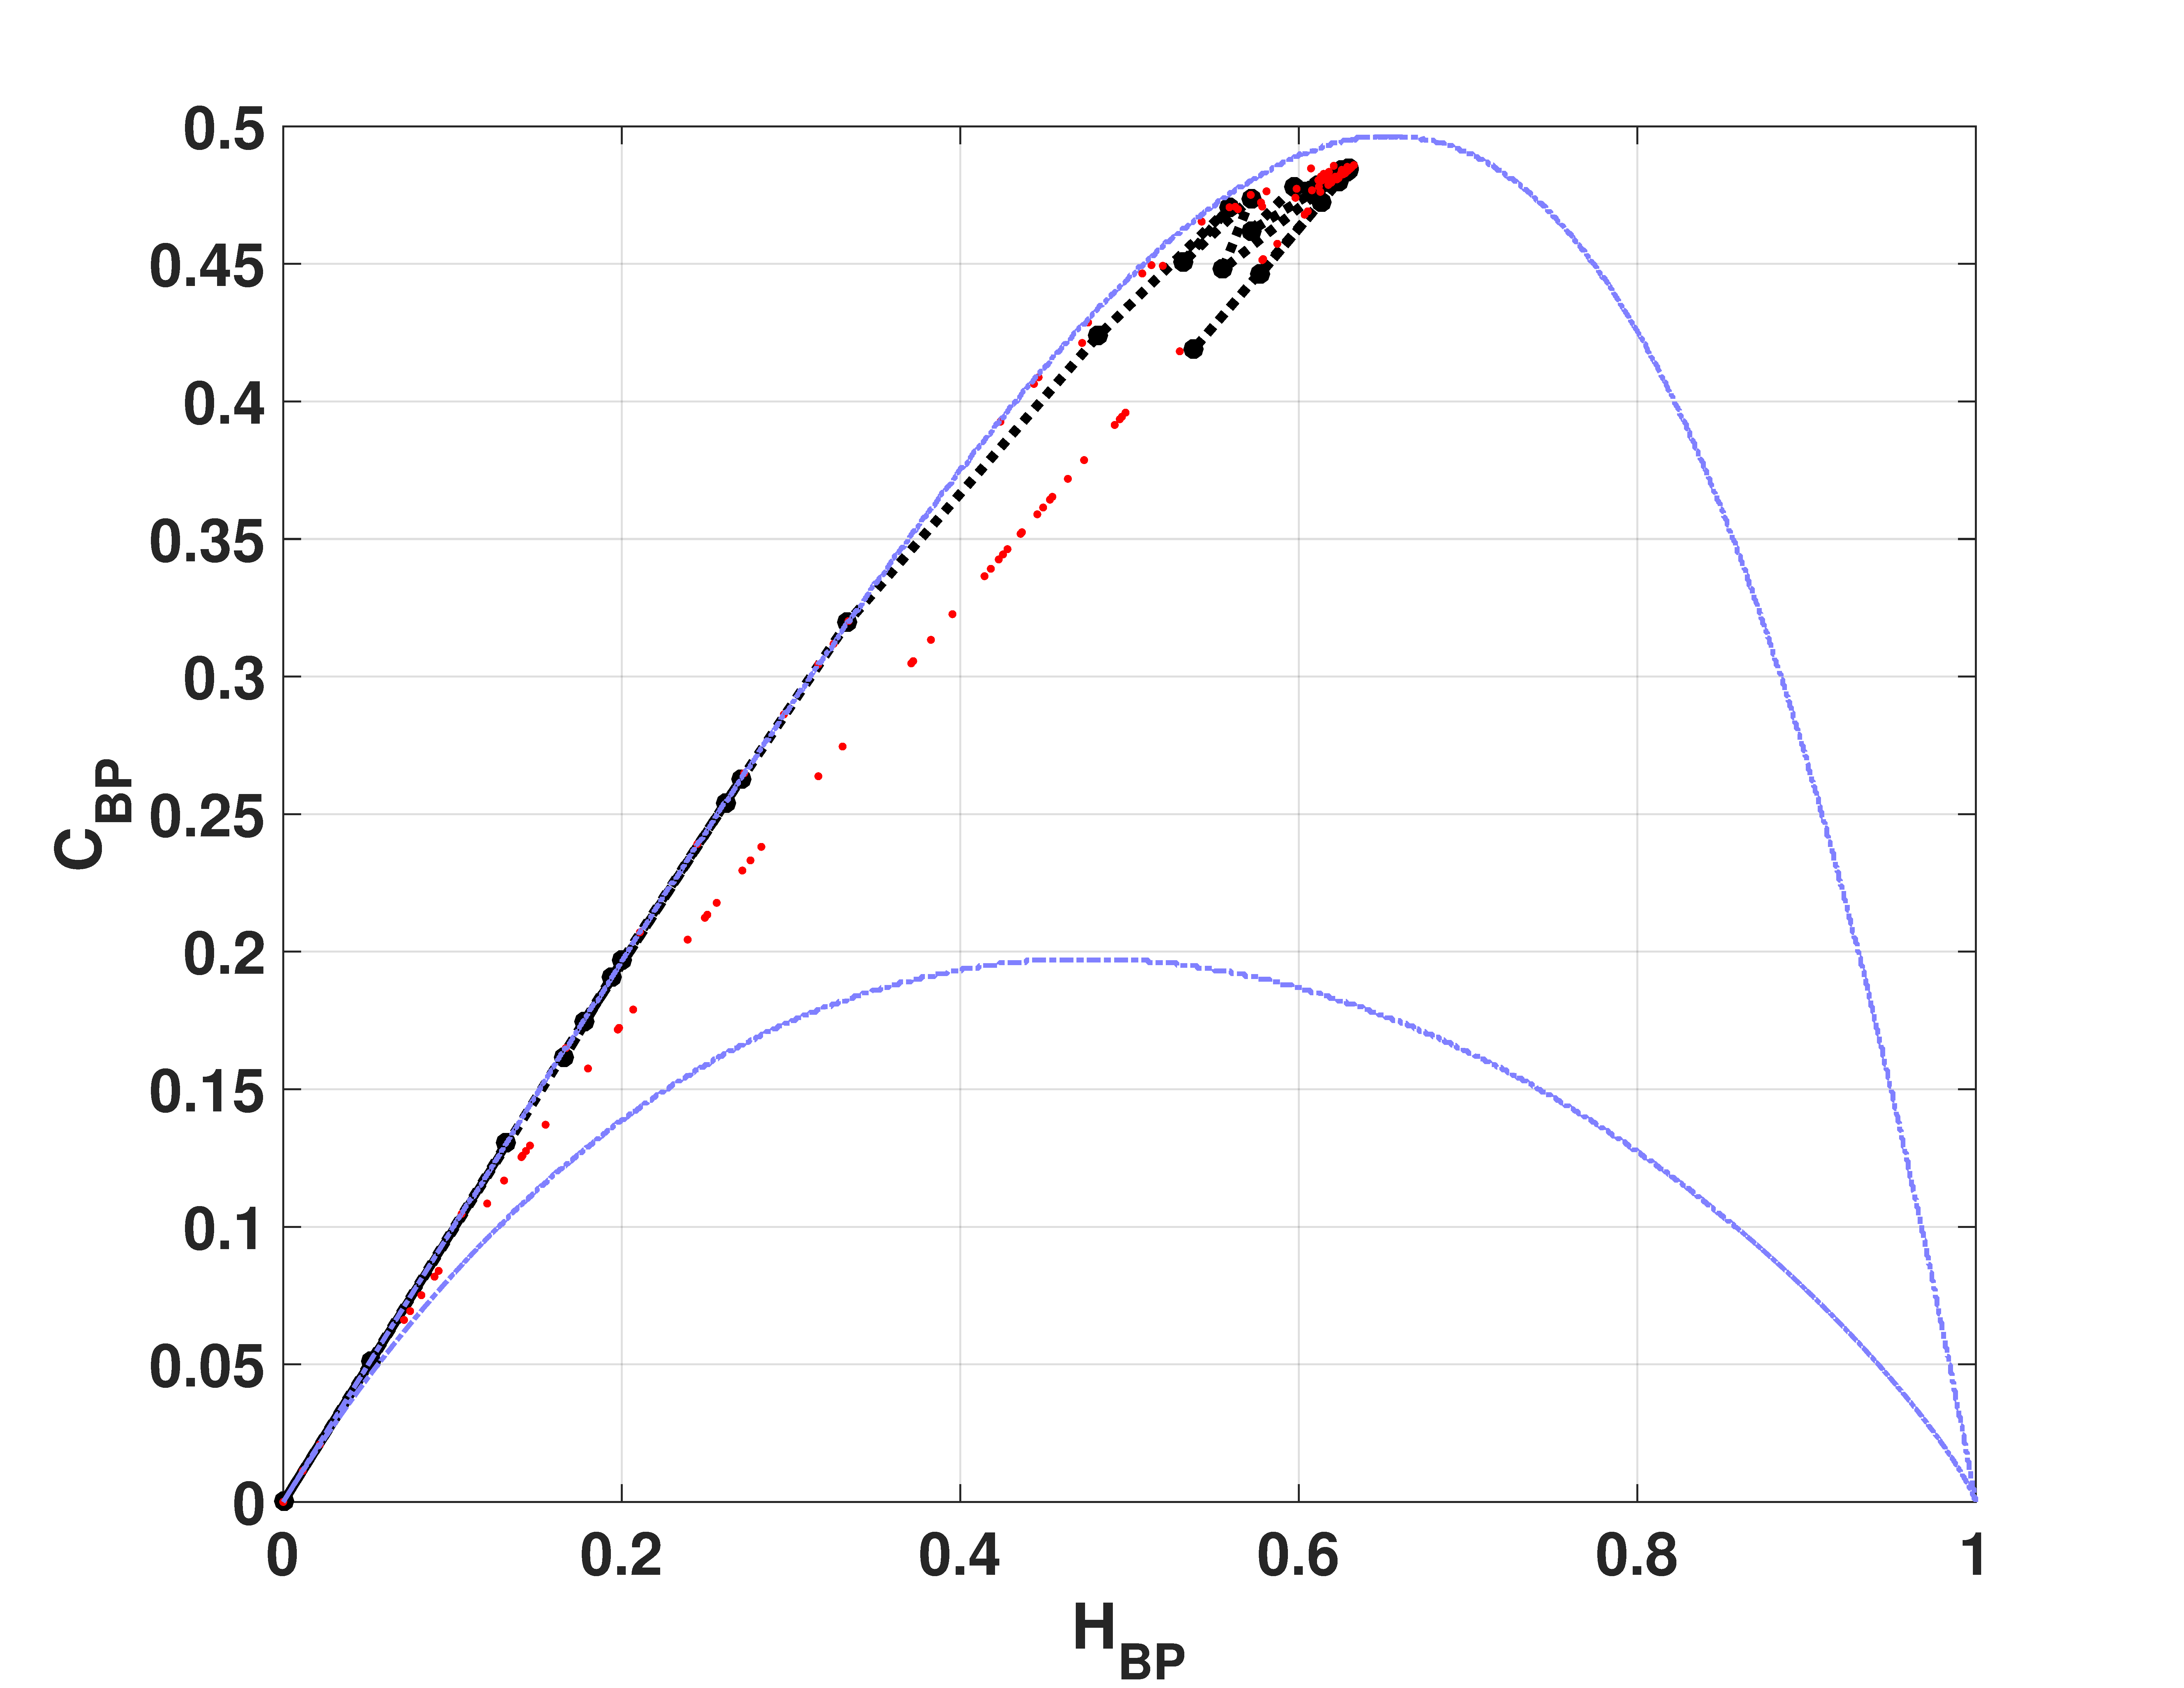
\includegraphics[width=.32\textwidth]{CbpHbp_LogisticoB2}
	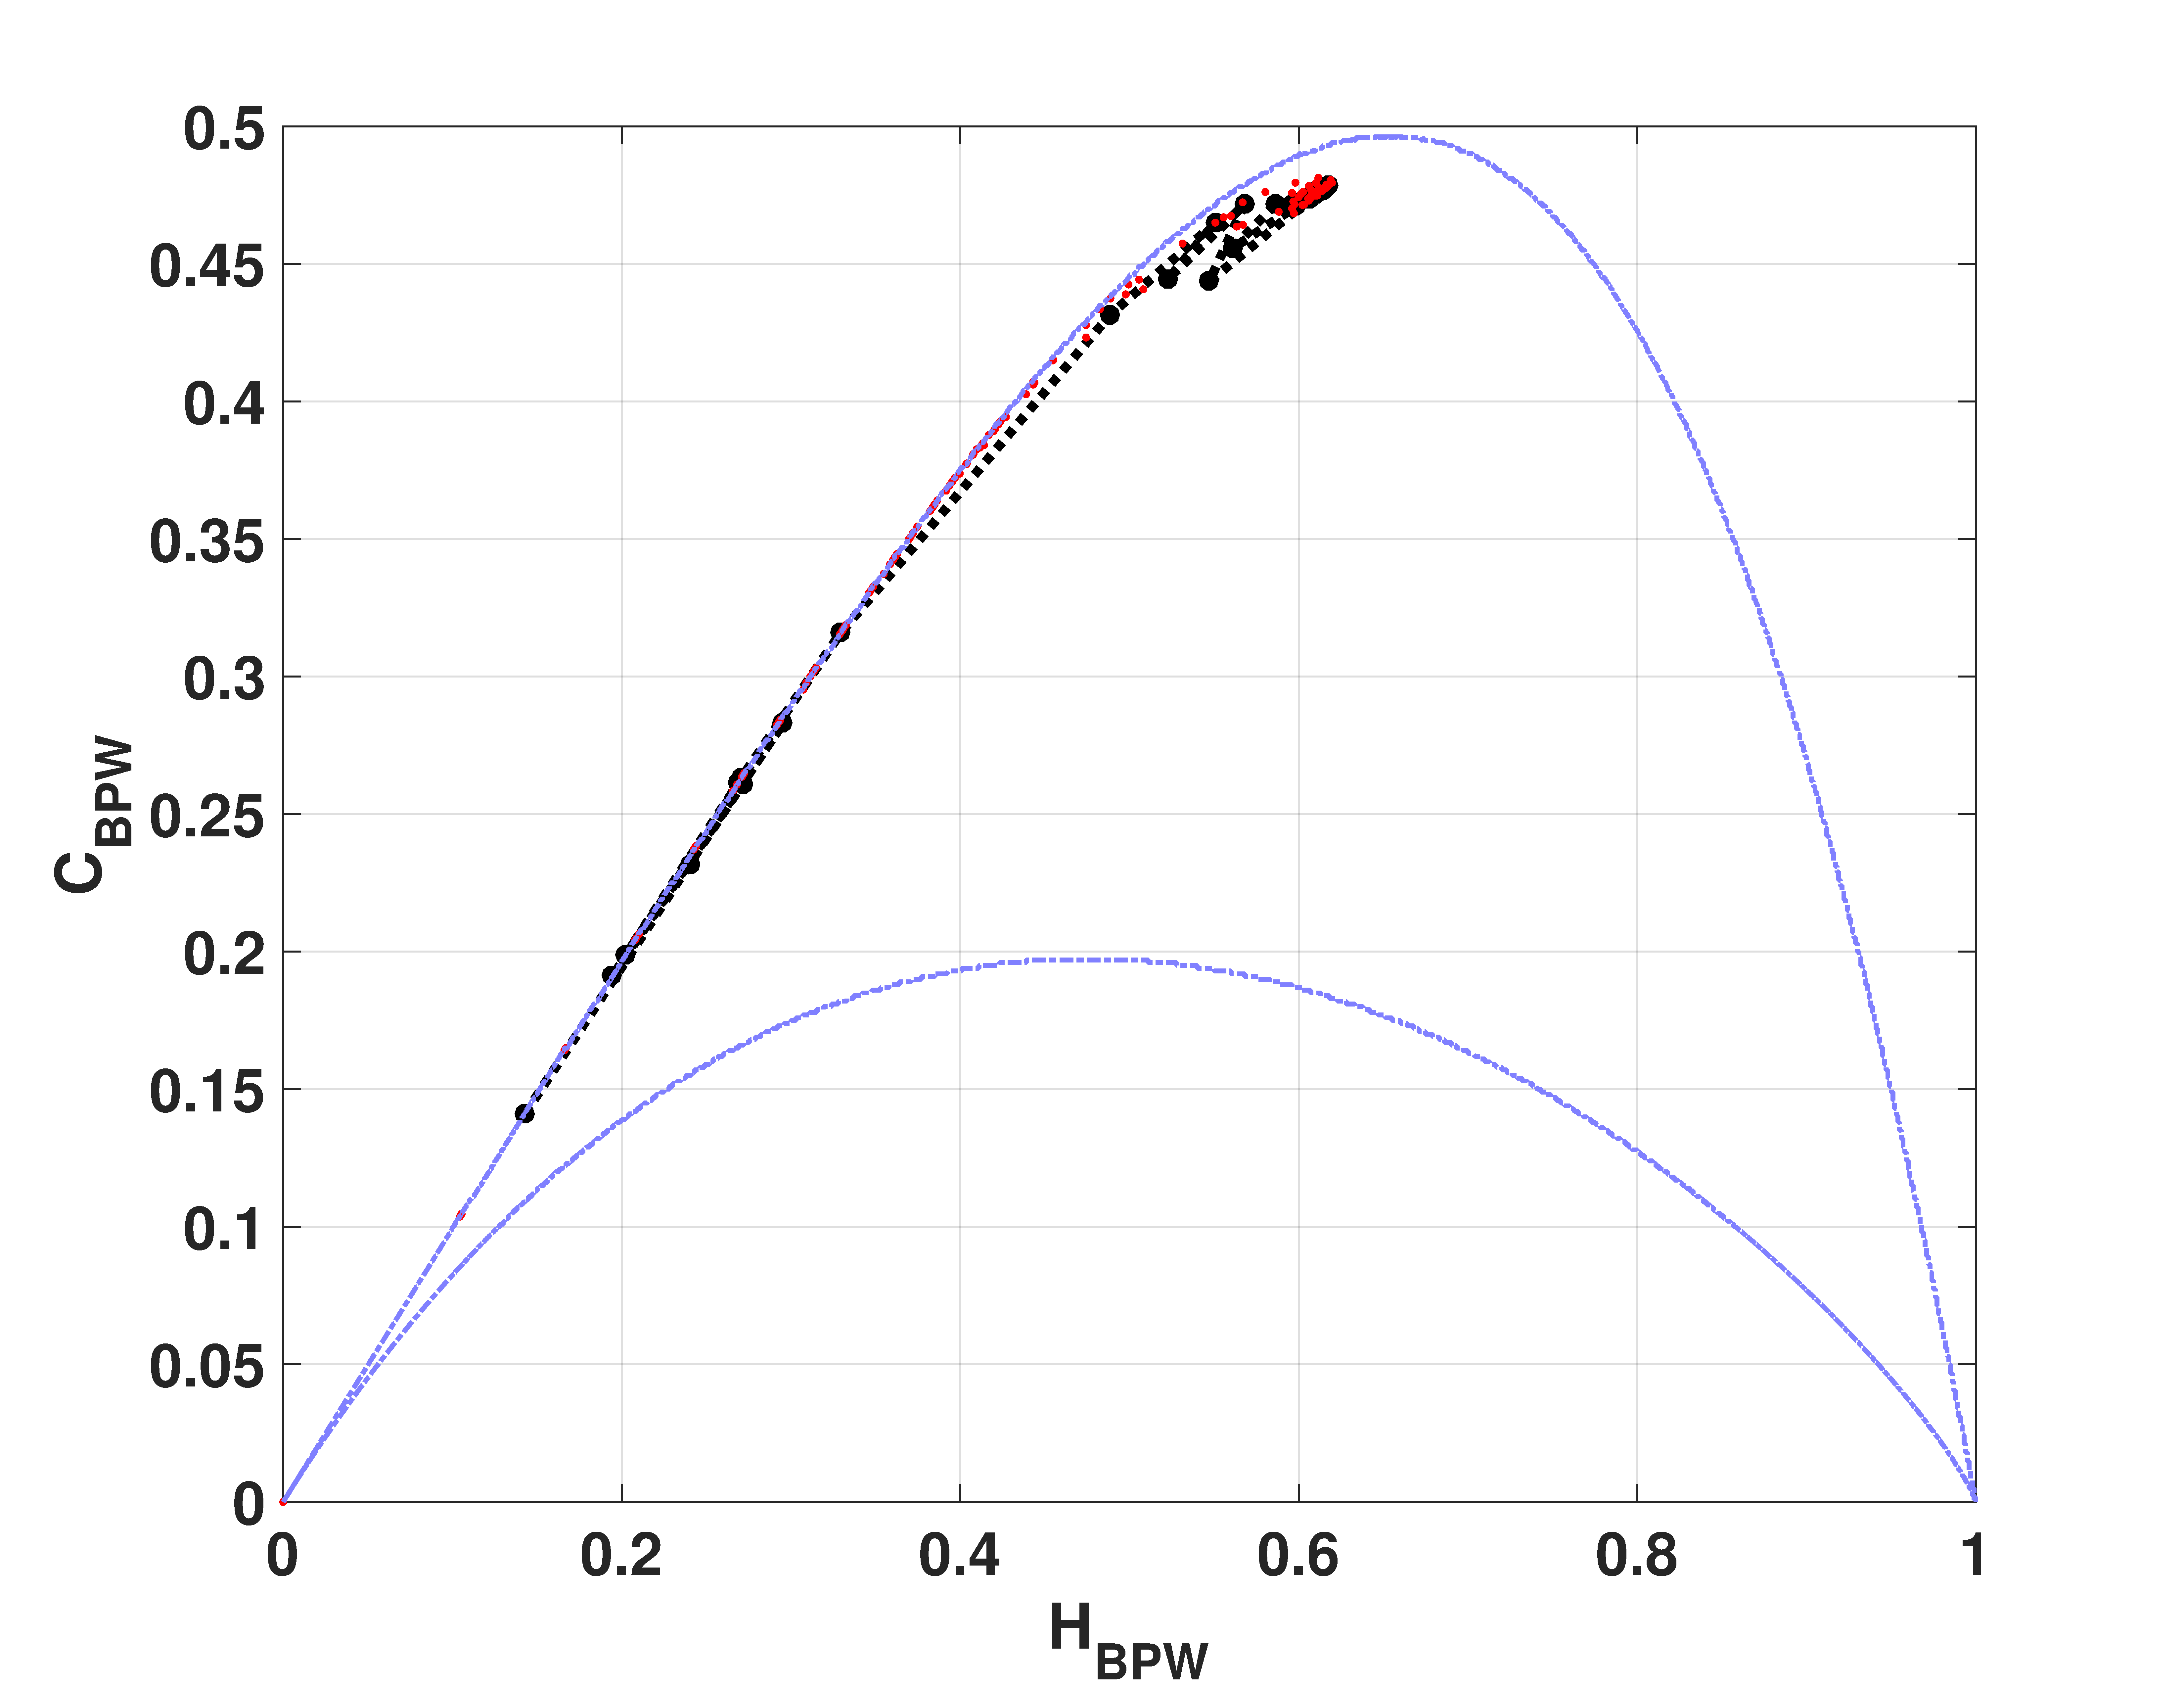
\includegraphics[width=.32\textwidth]{CbpwHbpw_LogisticoB2}
	\caption{Statistical properties of the LOG map using binary representation: (a) $H_{hist}$ vs $P$ (b) $H_{BP}$ vs $P$ (c) $C_{BP}$ vs $P$ (d) Number of missing ordering patterns $MP$ vs $P$. In Figures (a) to (d) dashed line correspond to floating point numbers. (d) representation in the $H_{hist},H_{BP}$ plane in the the decimal numerical system.  The star represents the state for floating points numbers. (e) representation in the $H_{hist},H_{BP}$ plane. The star represents the state for floating point numbers; (f) representation in the $H_{BP},C_{BP}$ plane.  The star represents the state for floating points numbers. (f) representation in the $H_{BP},C_{BP}$ plane for binary numerical system.  The star represents the state for floating points numbers. } \label{fig:LOGbinario}
\end{figure}

%%%%%%%%%%%%%%%%%%%%%%%%%%
%%%%%%%%%%%%%%%%%%%%%%%%%%% Fig.5
%\begin{figure}
%	\includegraphics[width=0.3\textwidth]{Hval_switchB10}
%	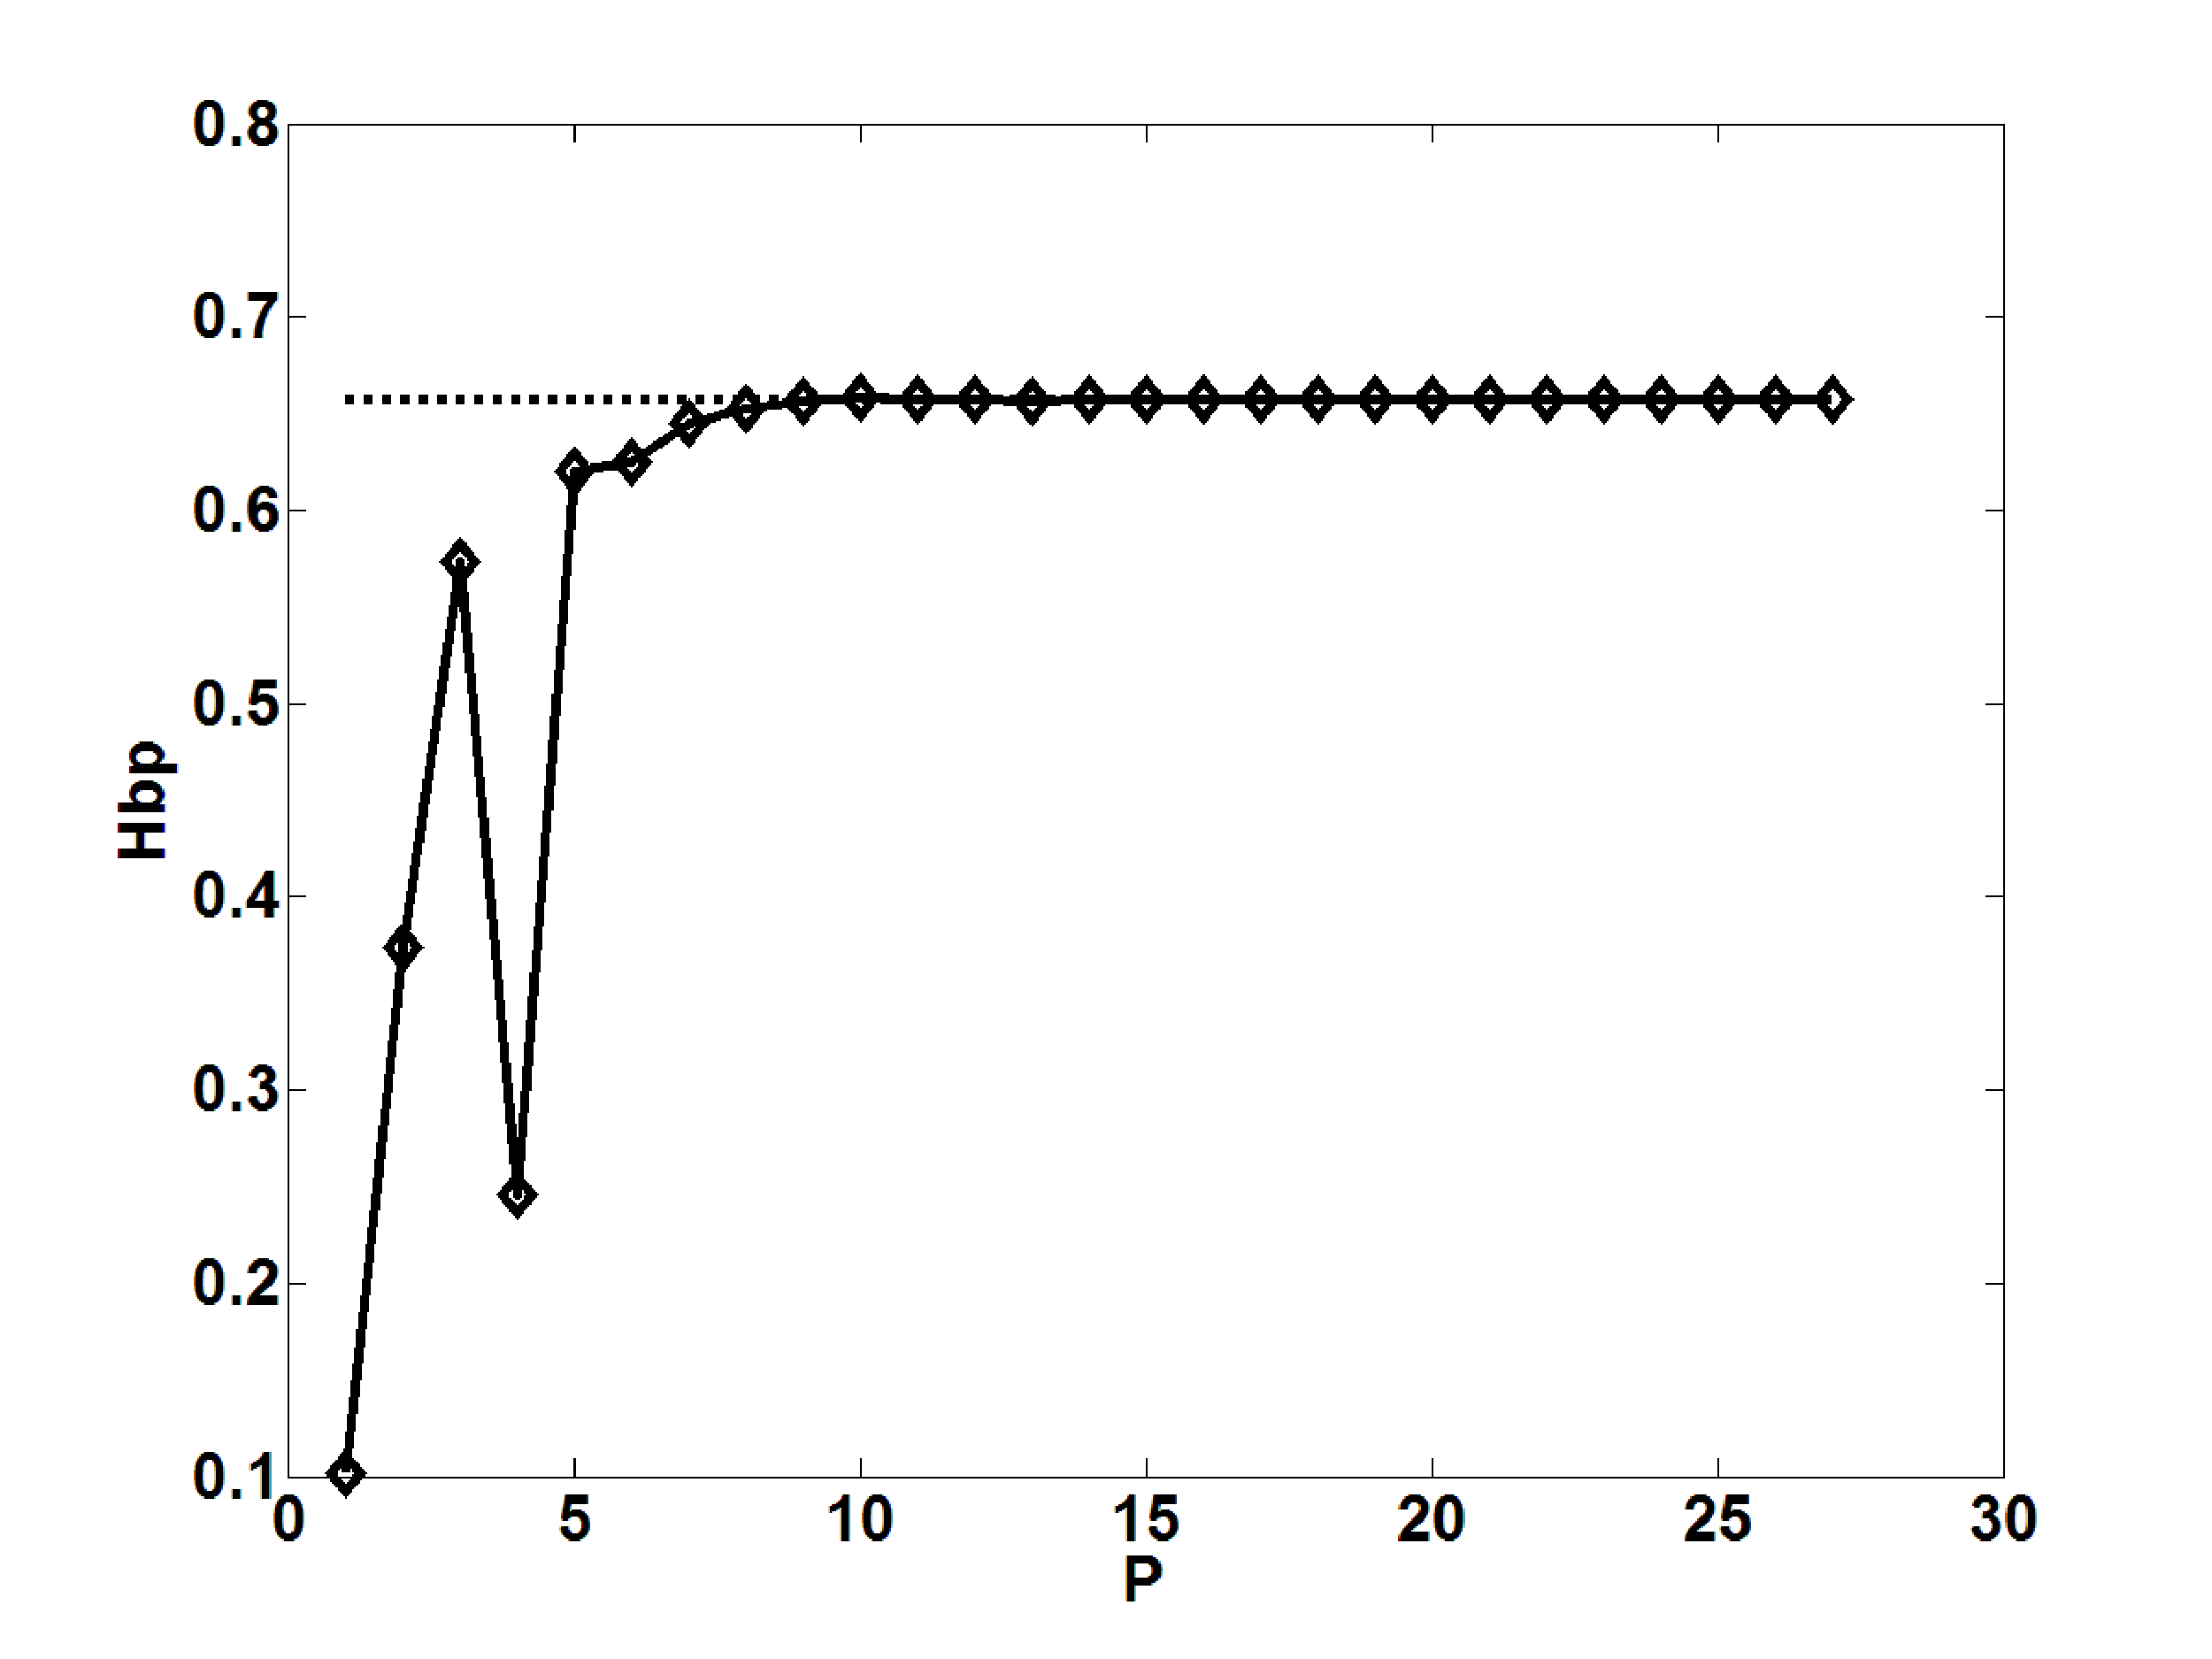
\includegraphics[width=0.3\textwidth]{Hbp_switchB10}
%	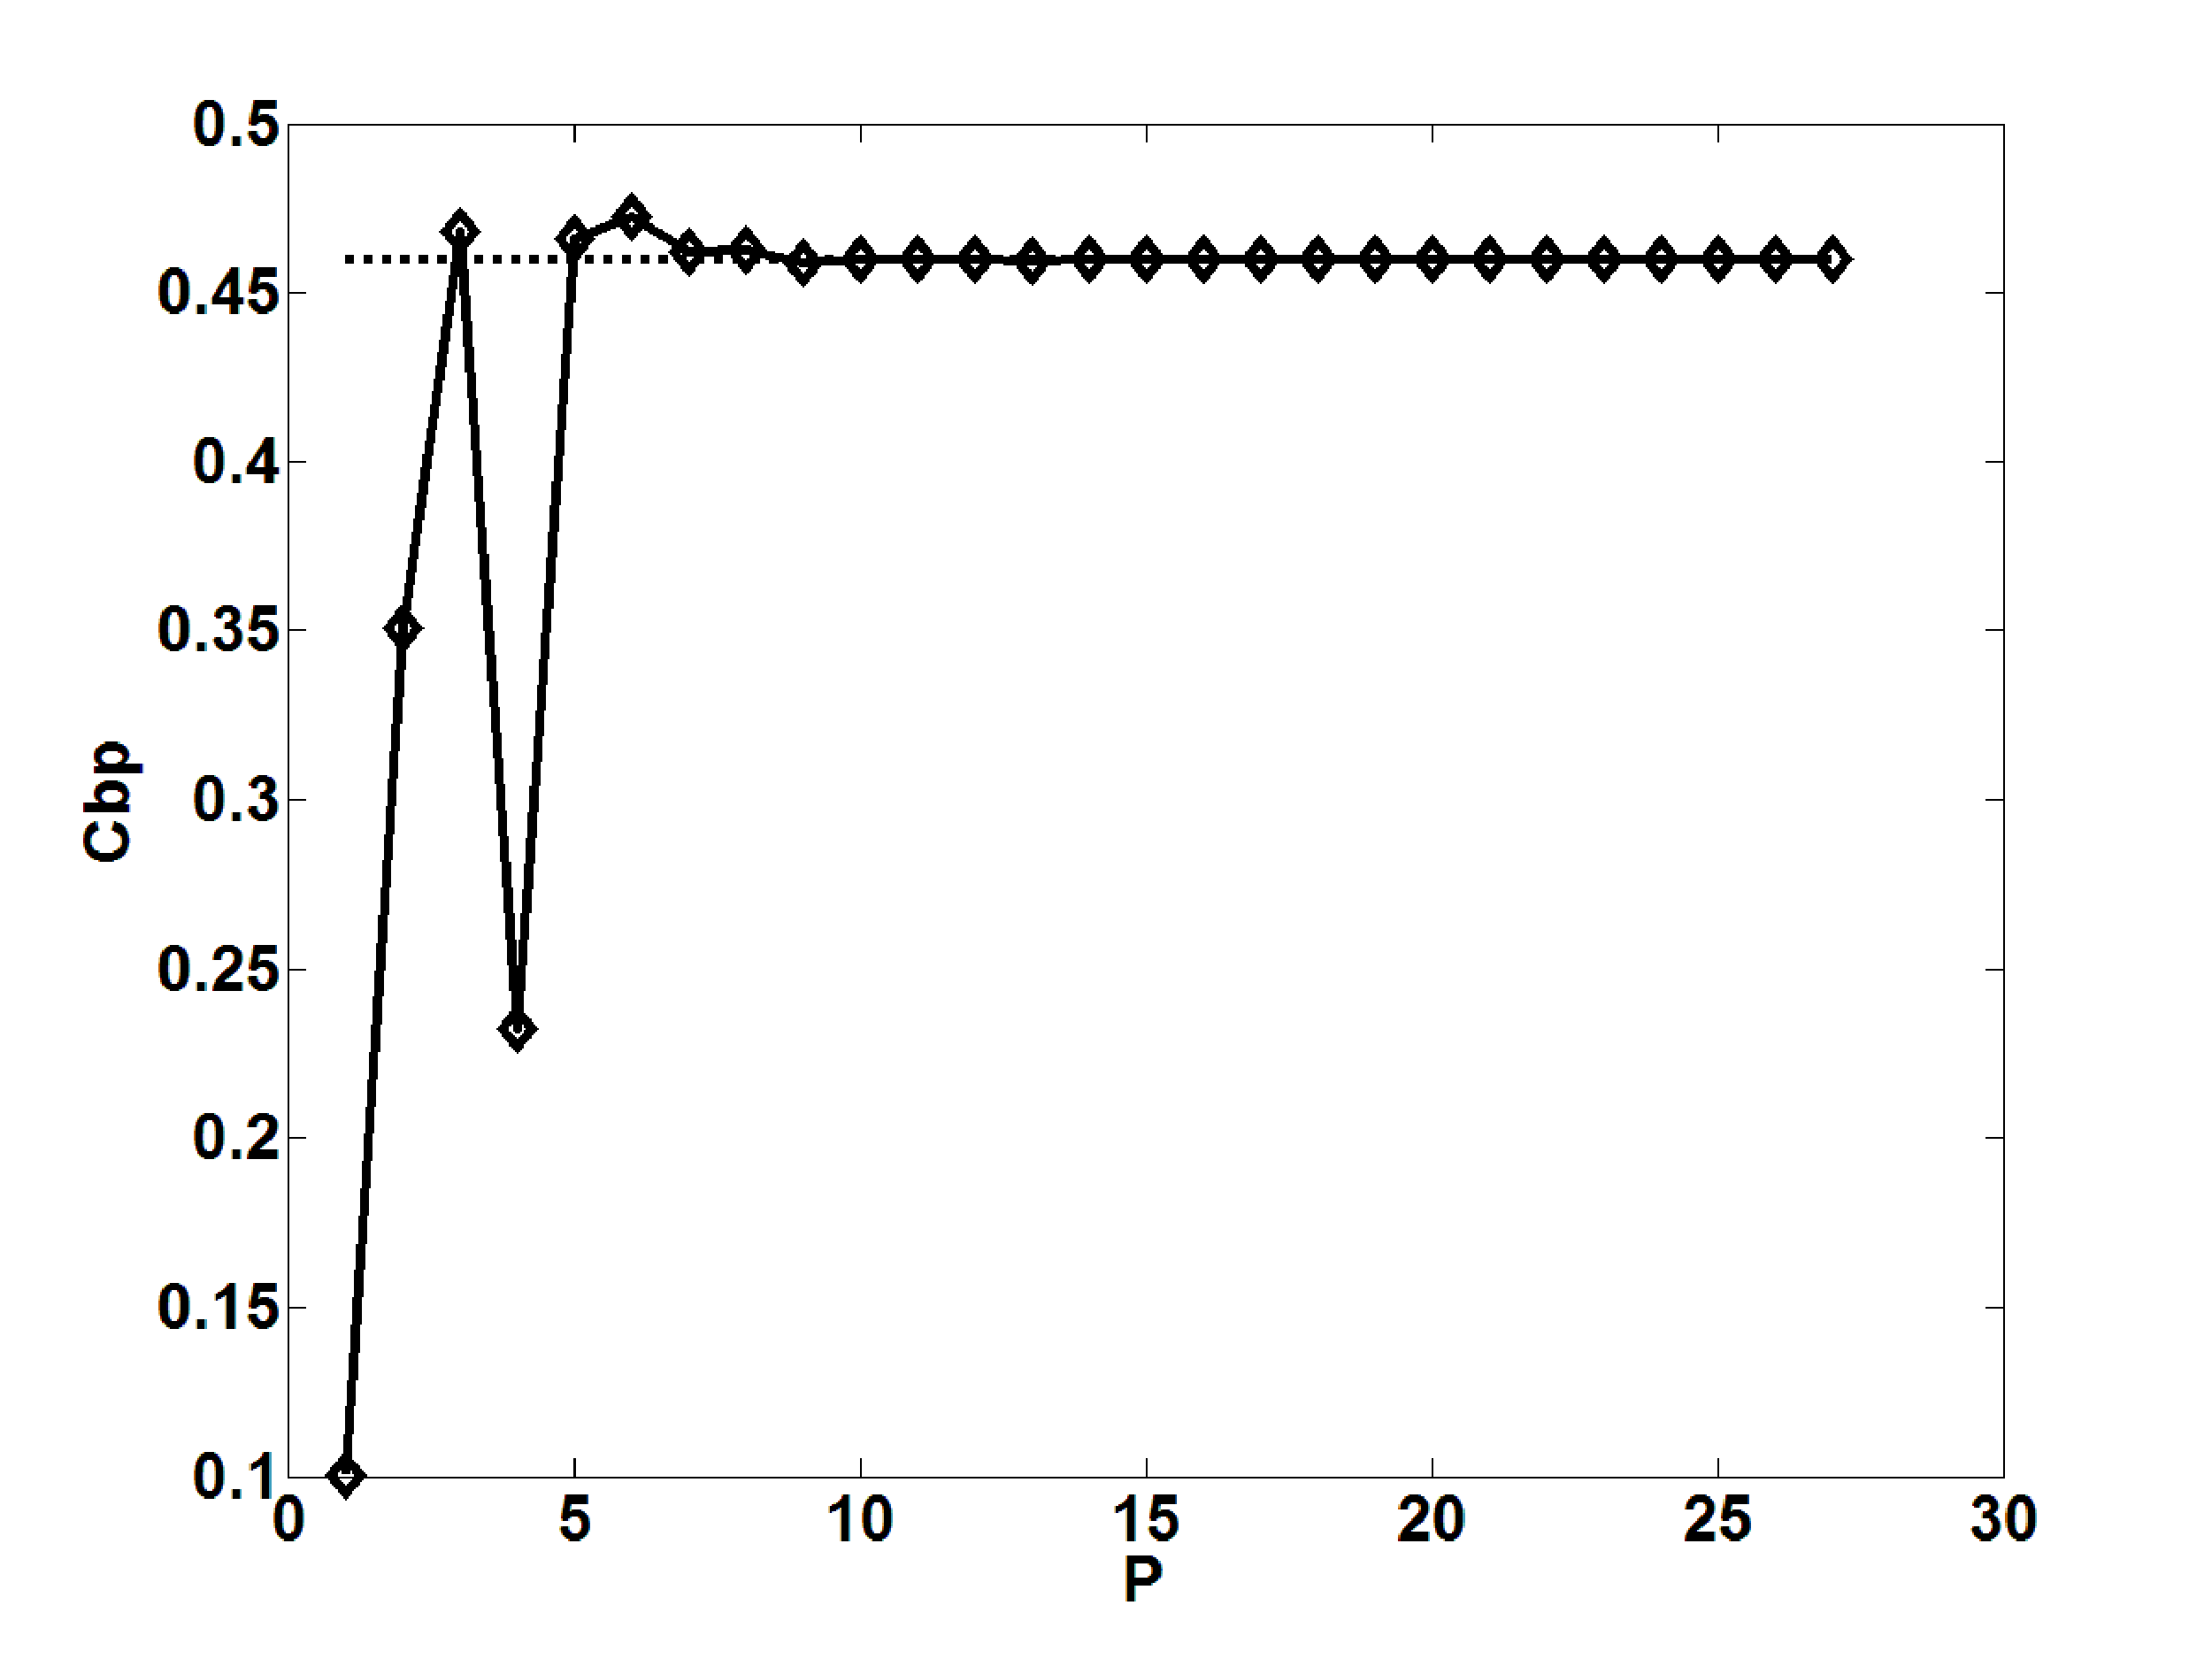
\includegraphics[width=0.3\textwidth]{Cbp_switchB10}
%	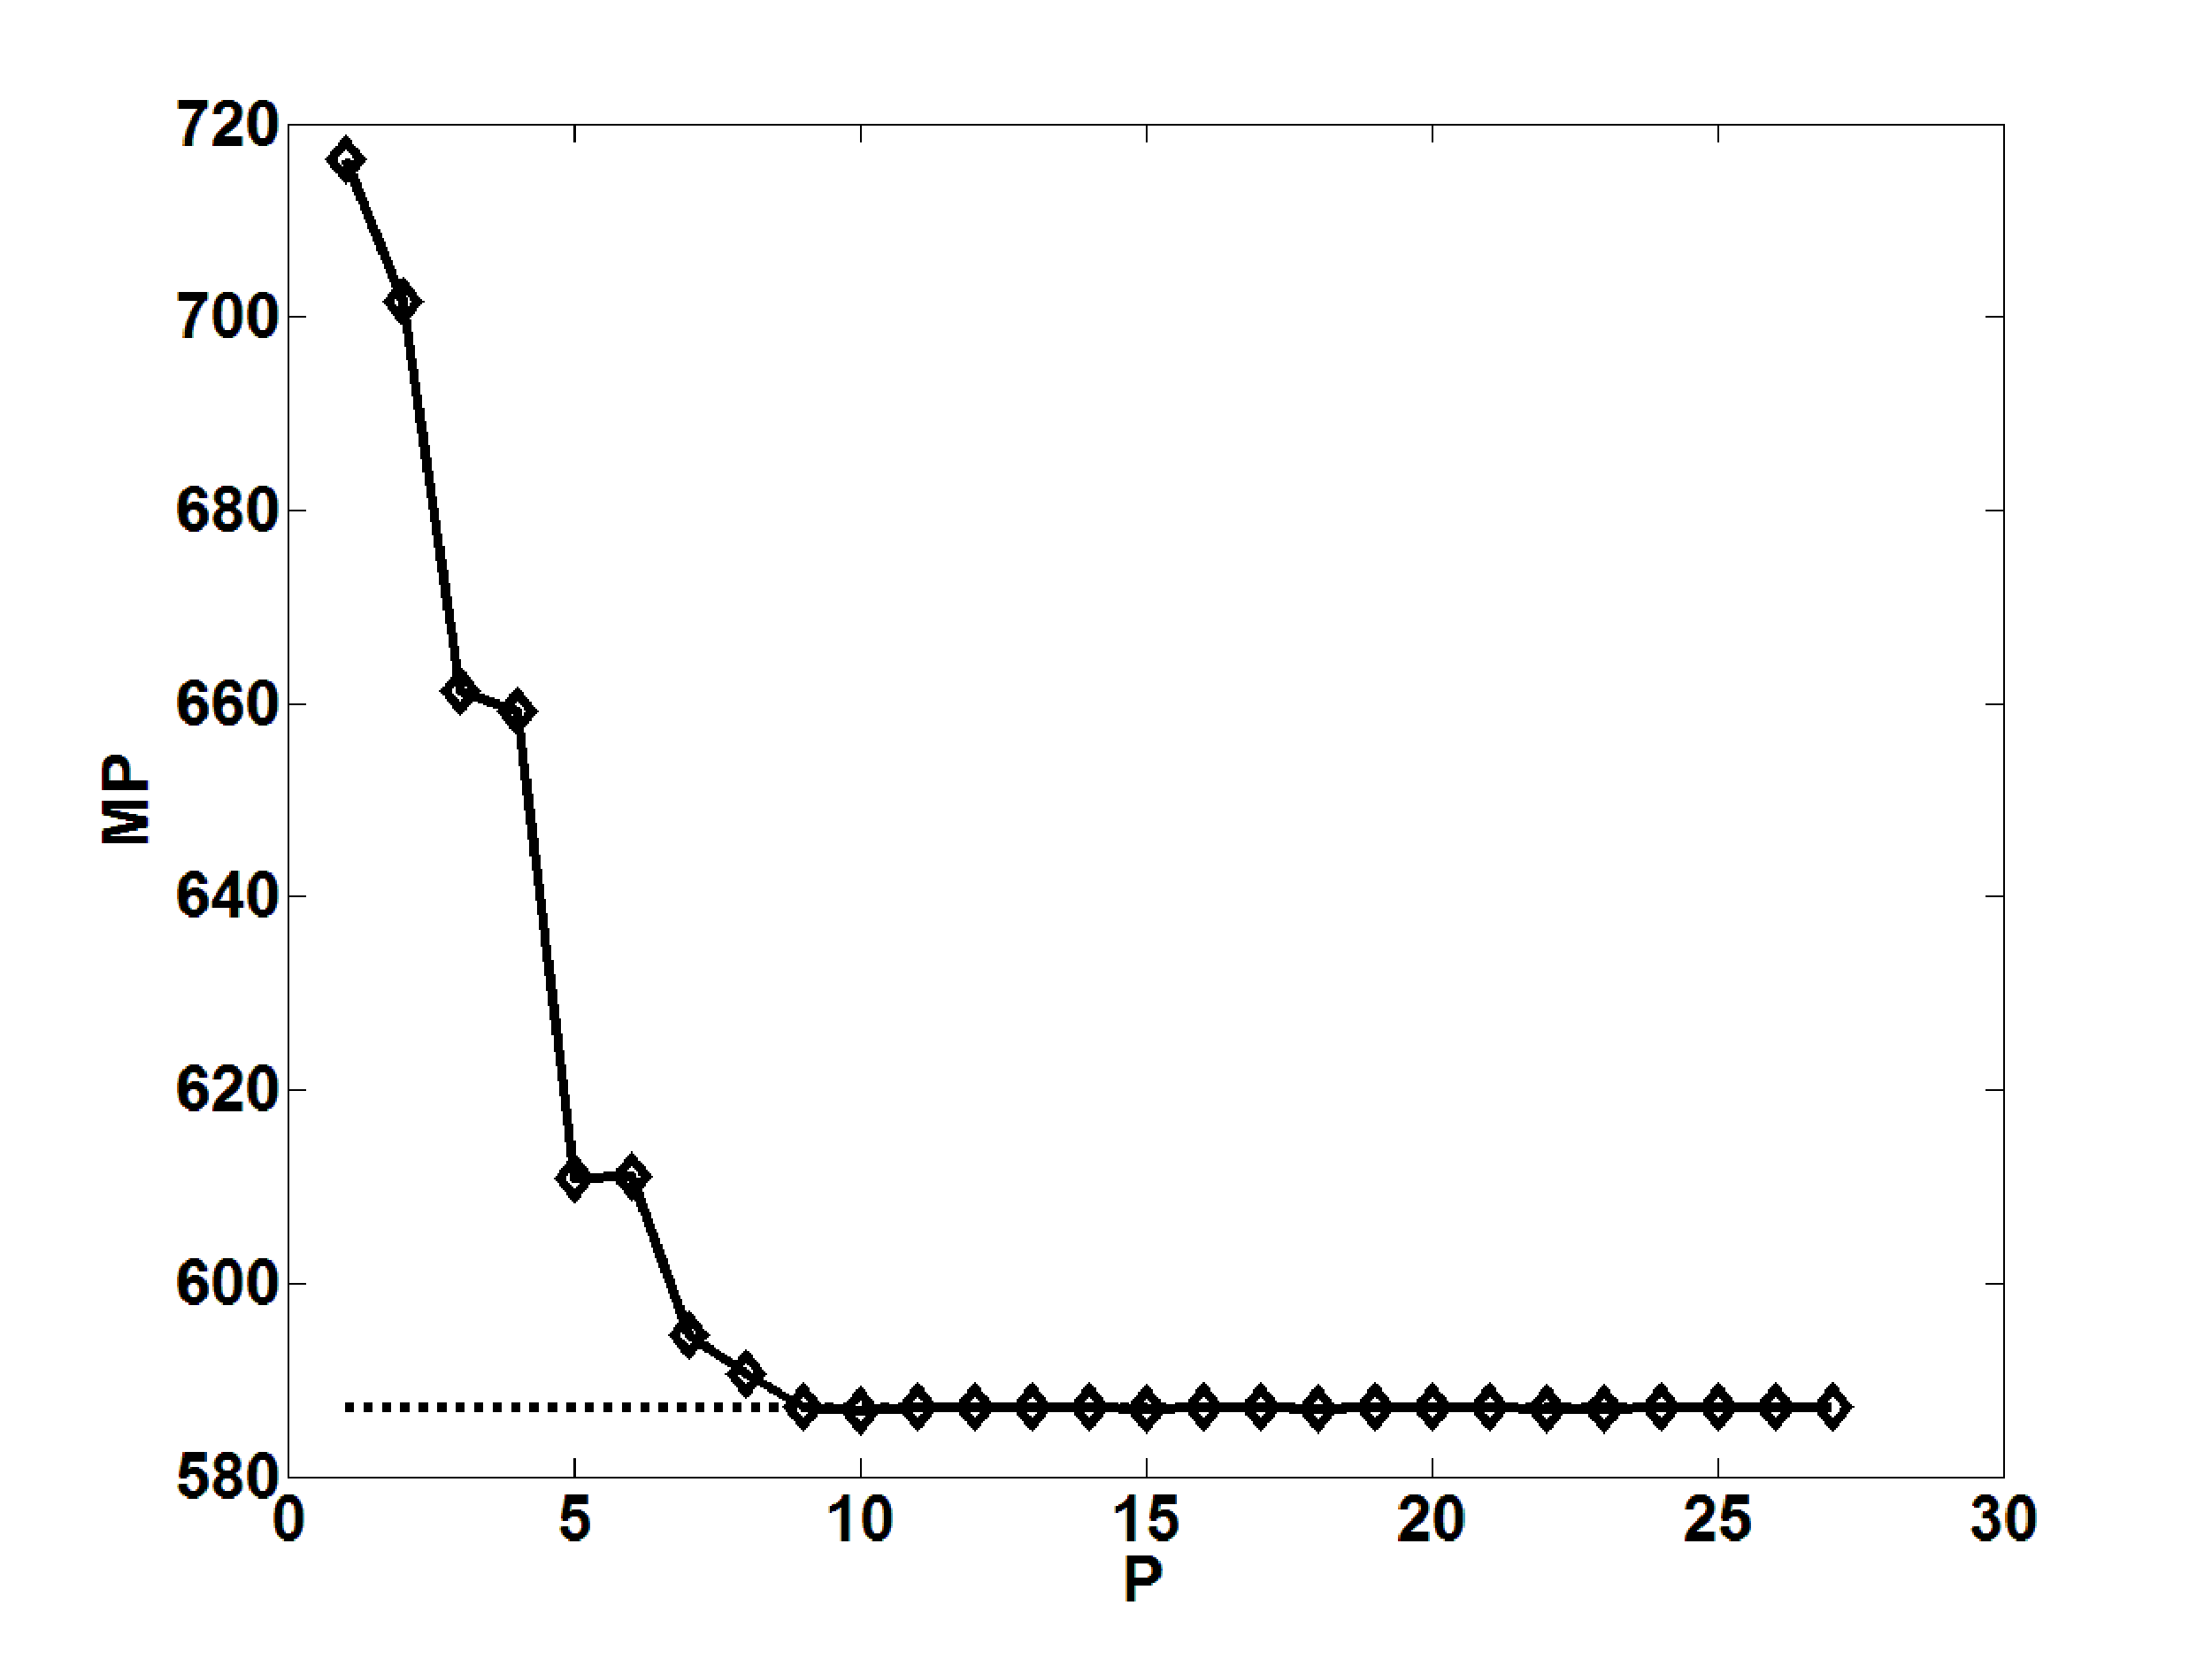
\includegraphics[width=0.3\textwidth]{Miss_switchB10}
%	\includegraphics[width=0.3\textwidth]{HvalHbp_switchB10}
%	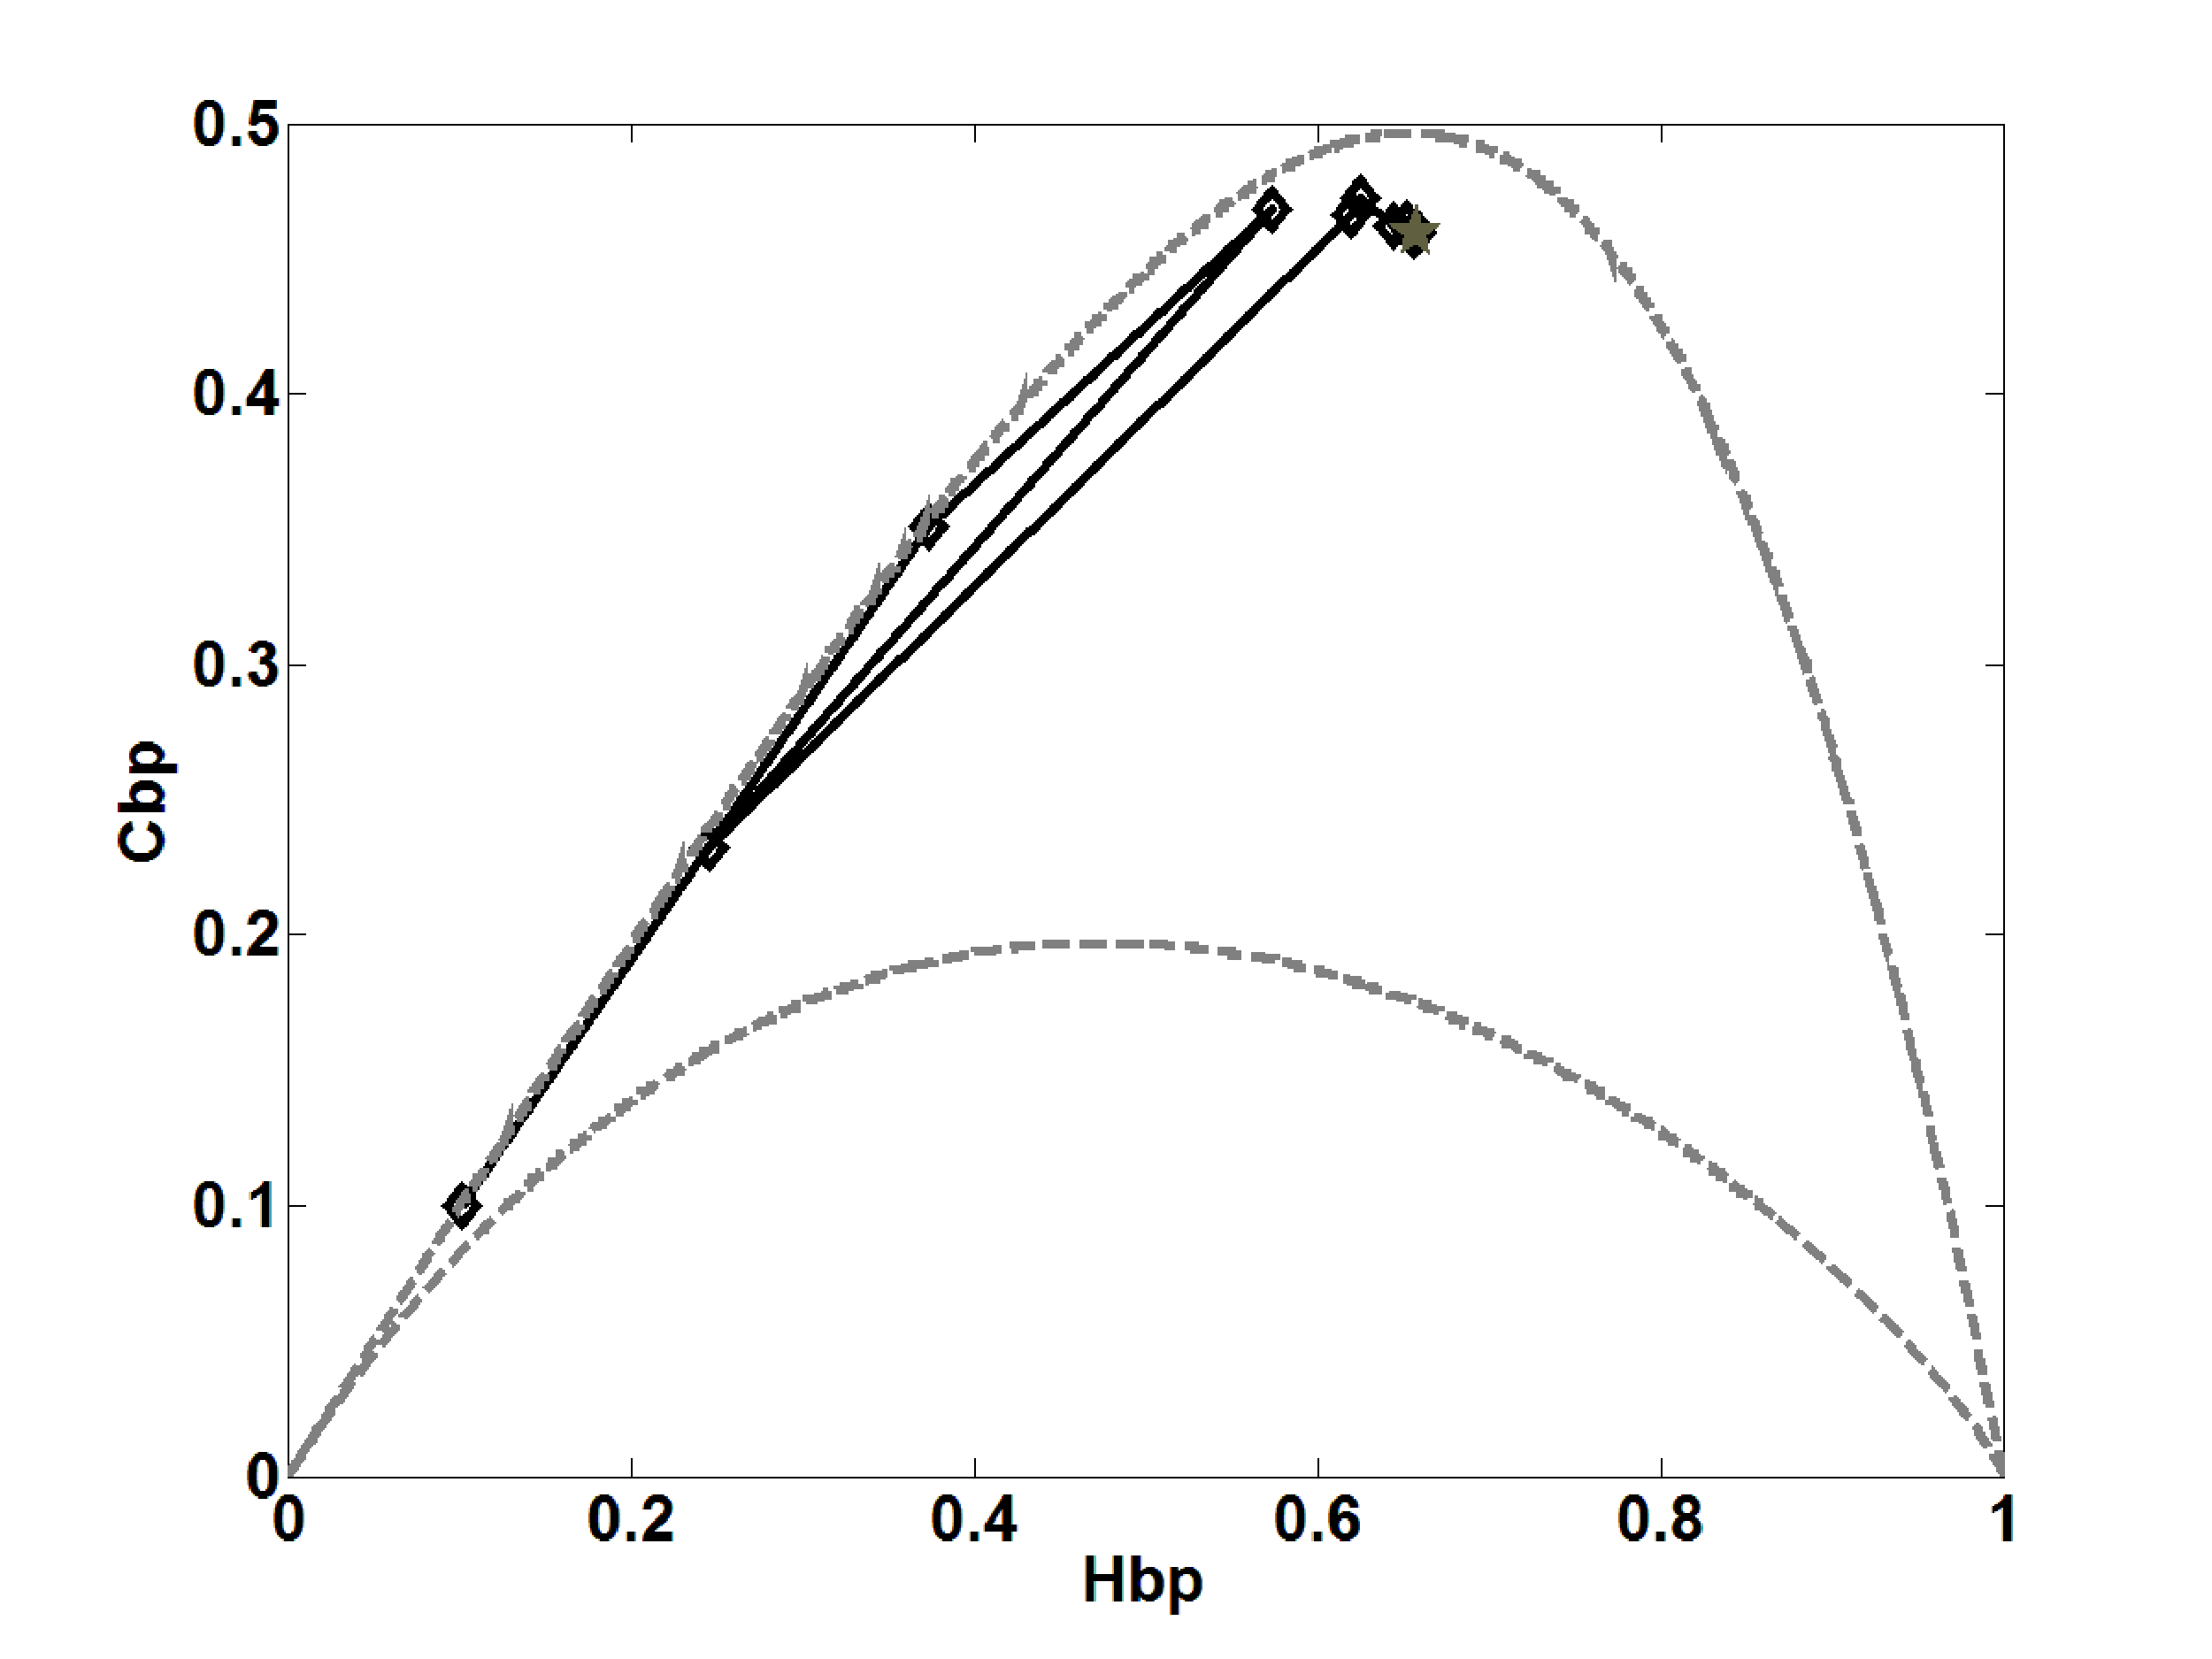
\includegraphics[width=0.3\textwidth]{HbpCbp_switchB10}
%	\caption{Statistical properties of the SWITCH map using decimal representation: (a) $H_{hist}$ vs $P$ (b) $H_{BP}$ vs $P$ (c) $C_{BP}$ vs $P$ (d) Number of missing ordering patterns $MP$ vs $P$. In Figures (a) to (d) dashed line correspond to floating point numbers. (e) representation in the $H_{hist},H_{BP}$ plane in the the decimal numerical system.  The star represents the state for floating points numbers. (f) representation in the $H_{BP},C_{BP}$ plane.  The star represents the state for floating points numbers. (The star represents the state for floating points numbers). } \label{fig:seqdec}
%\end{figure}

%%%%%%%%%%%%%%%%%%%%%%%%%%
%%%%%%%%%%%%%%%%%%%%%%%%%%% Fig.6
\begin{figure}
	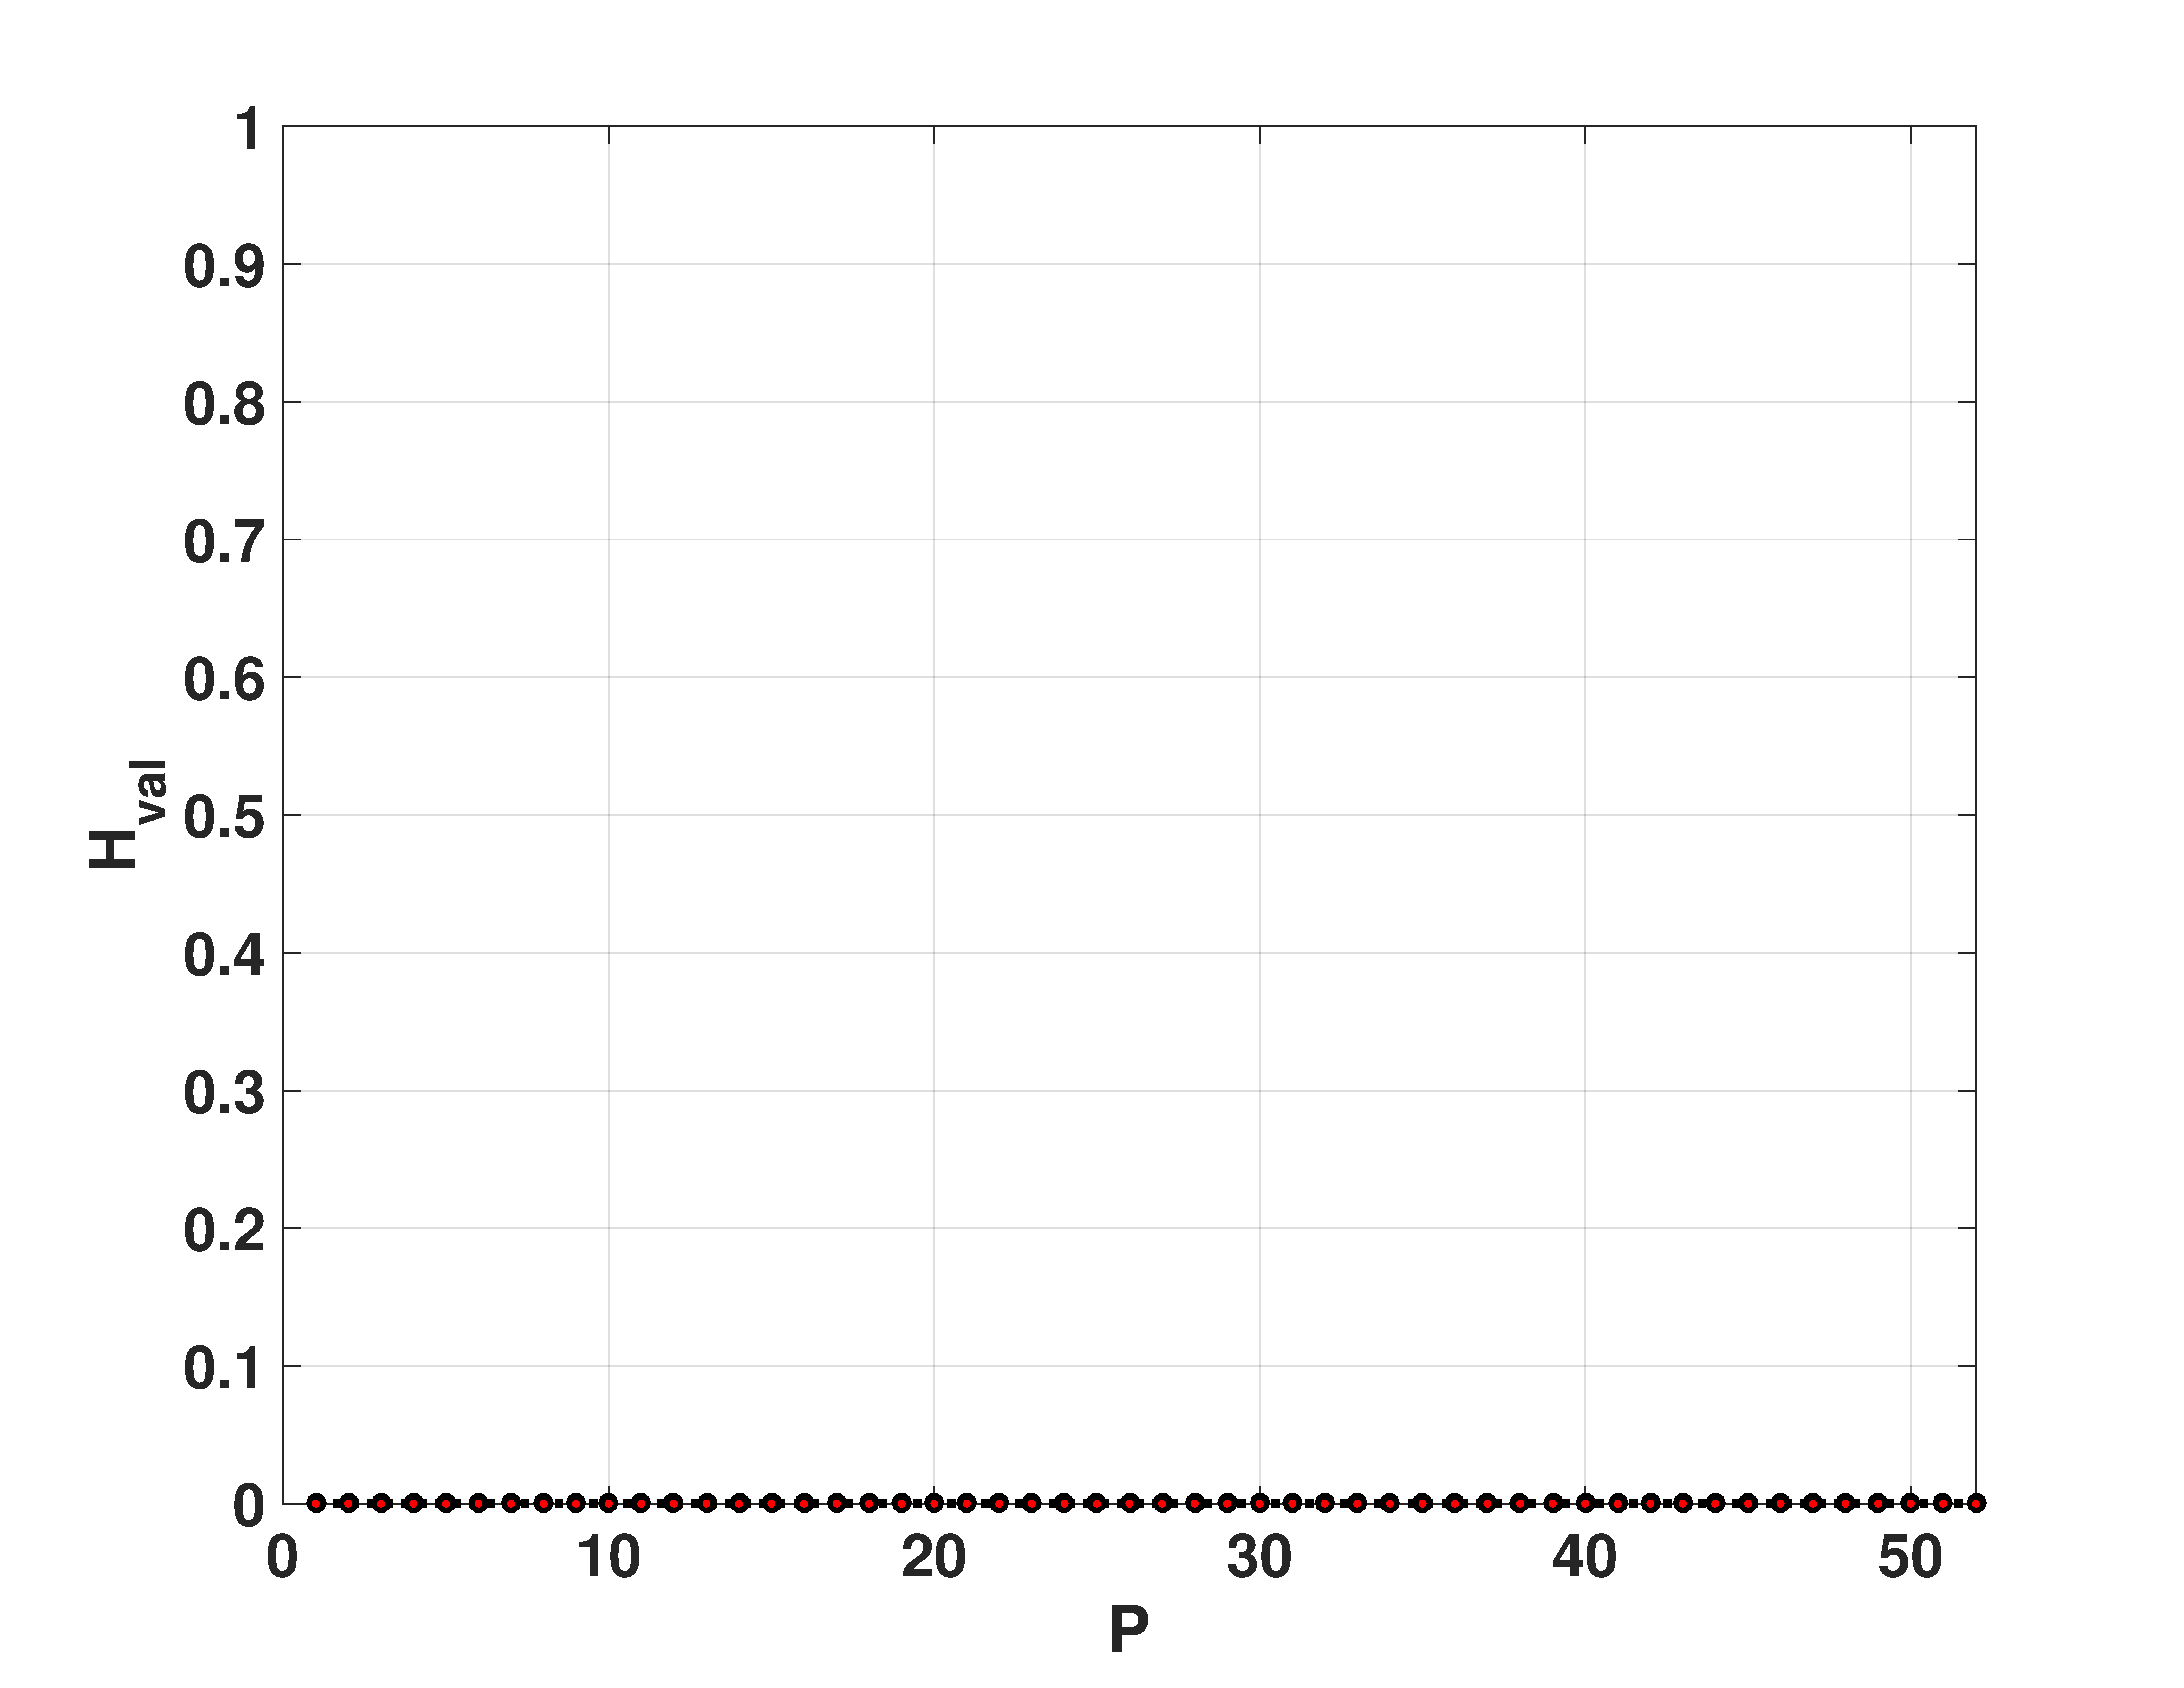
\includegraphics[width=.32\textwidth]{Hval_TentB2}
	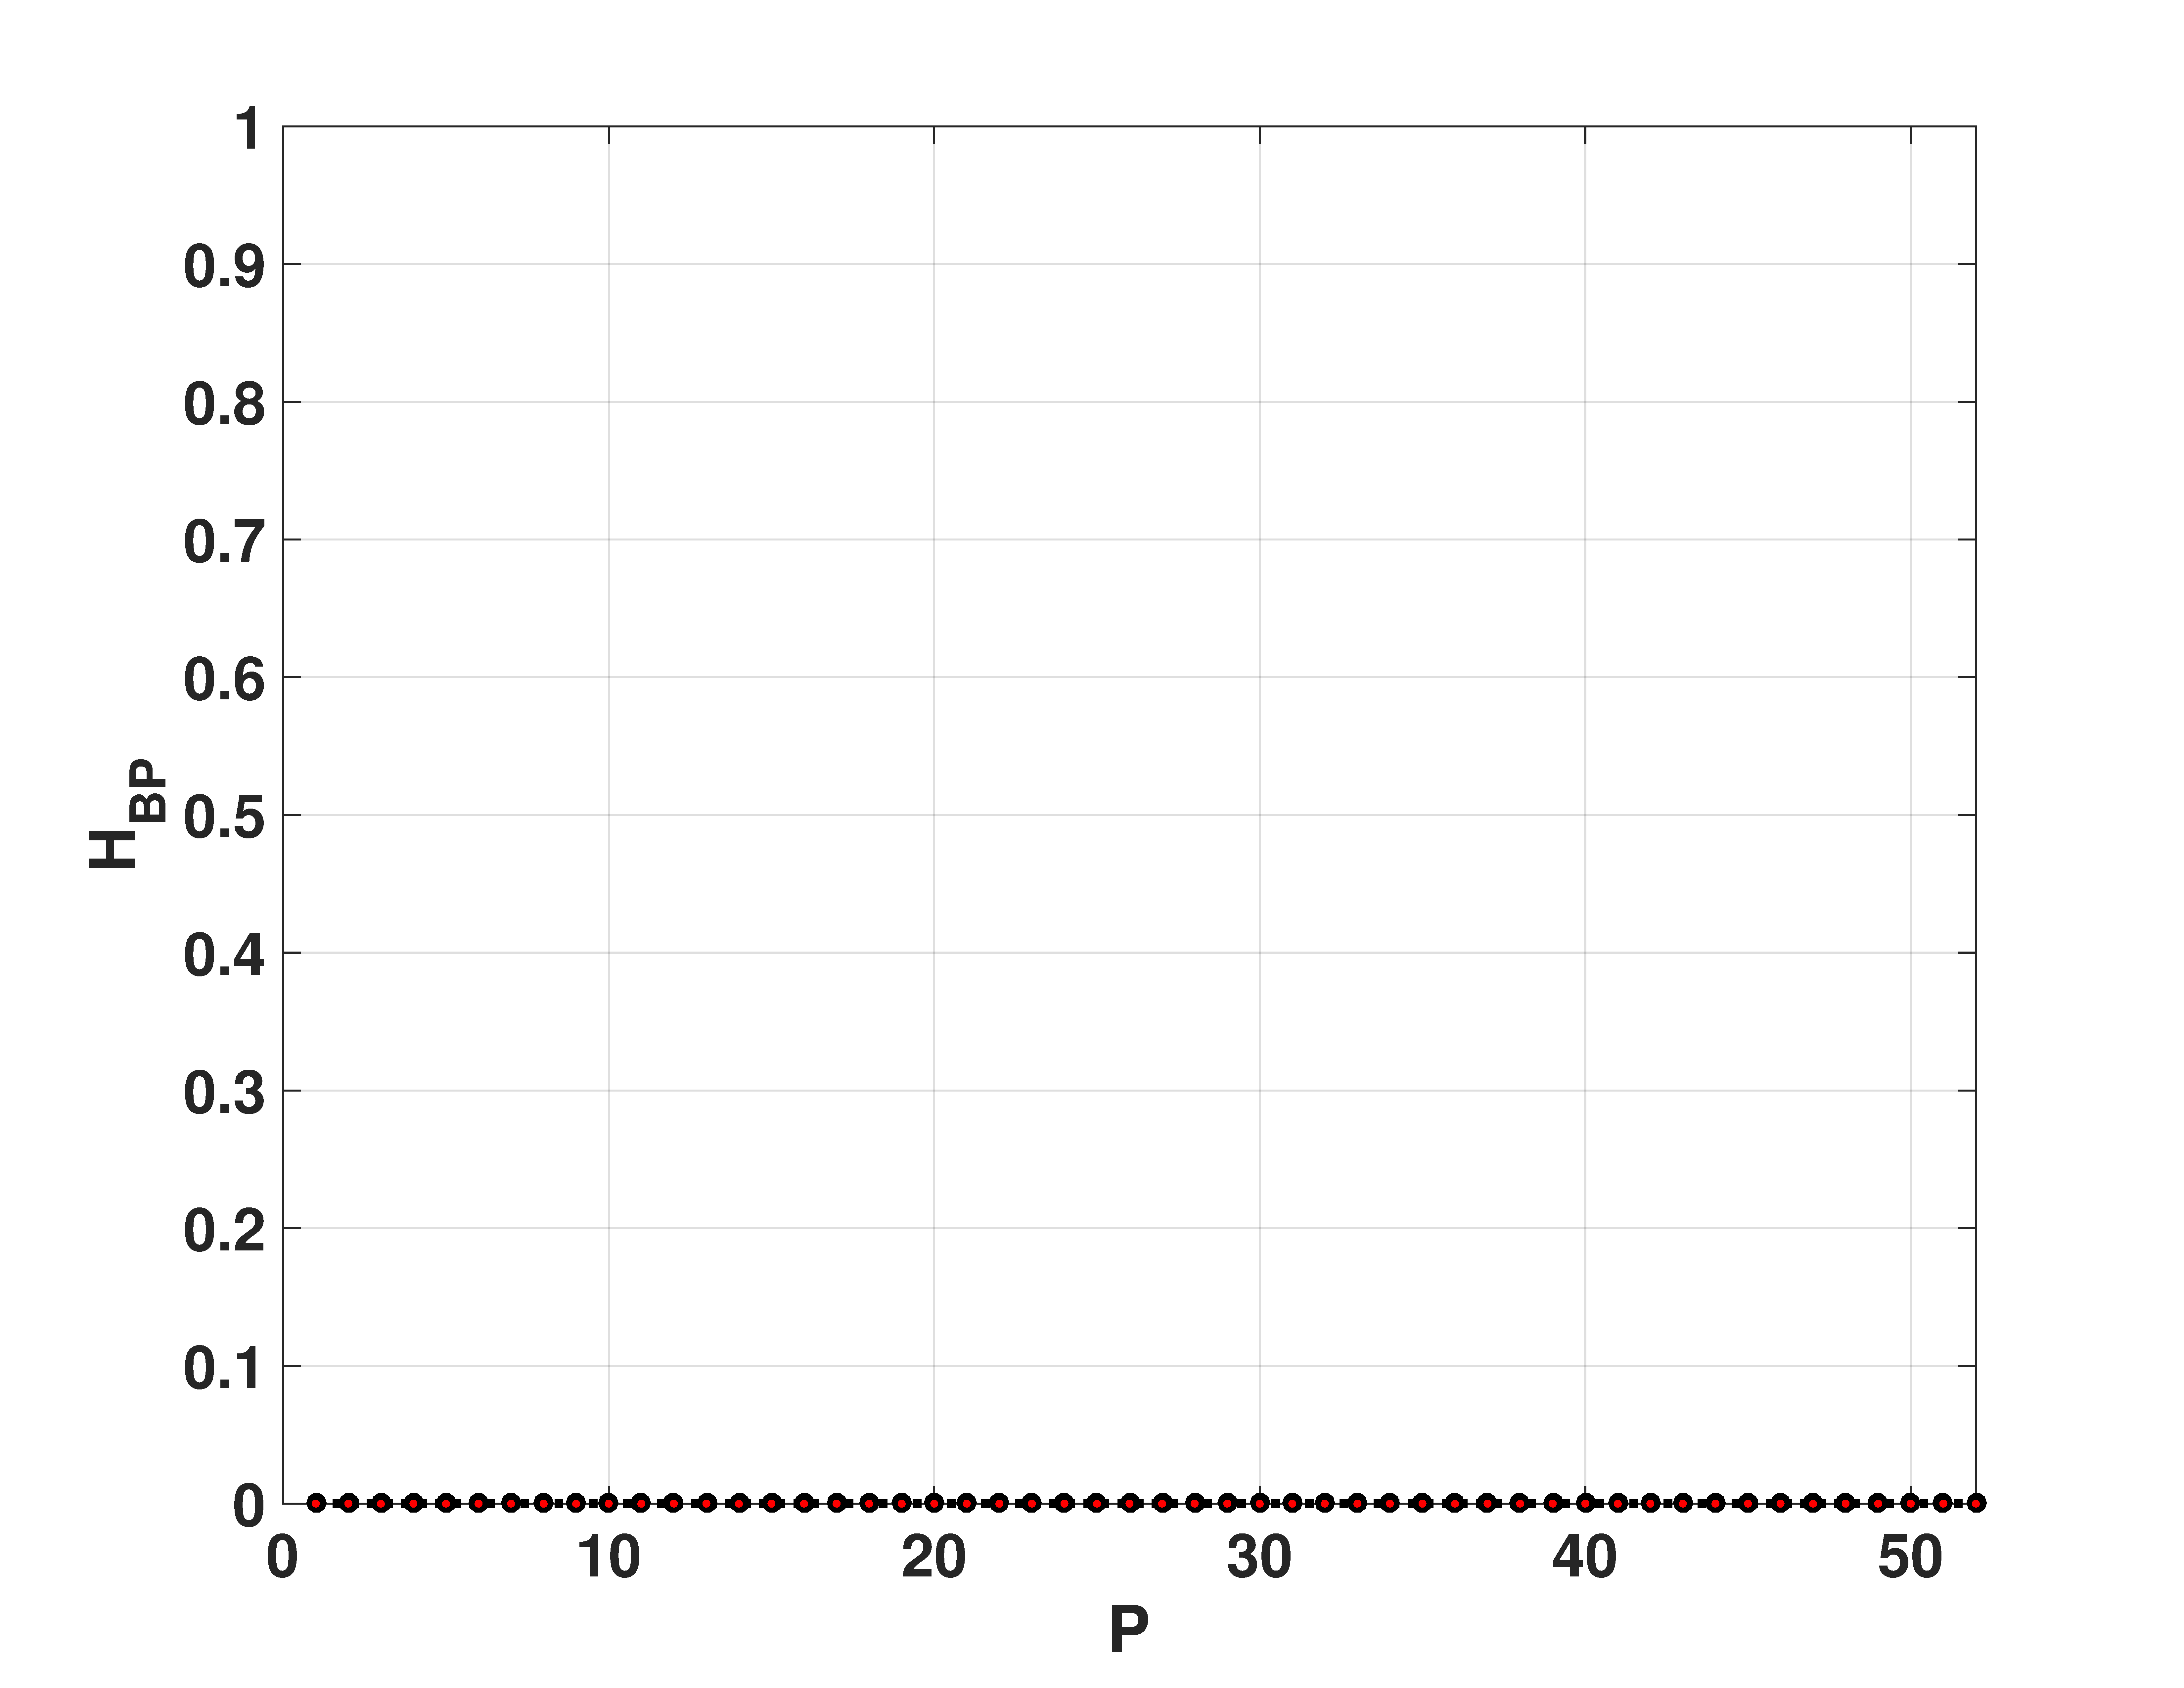
\includegraphics[width=.32\textwidth]{Hbp_TentB2}
	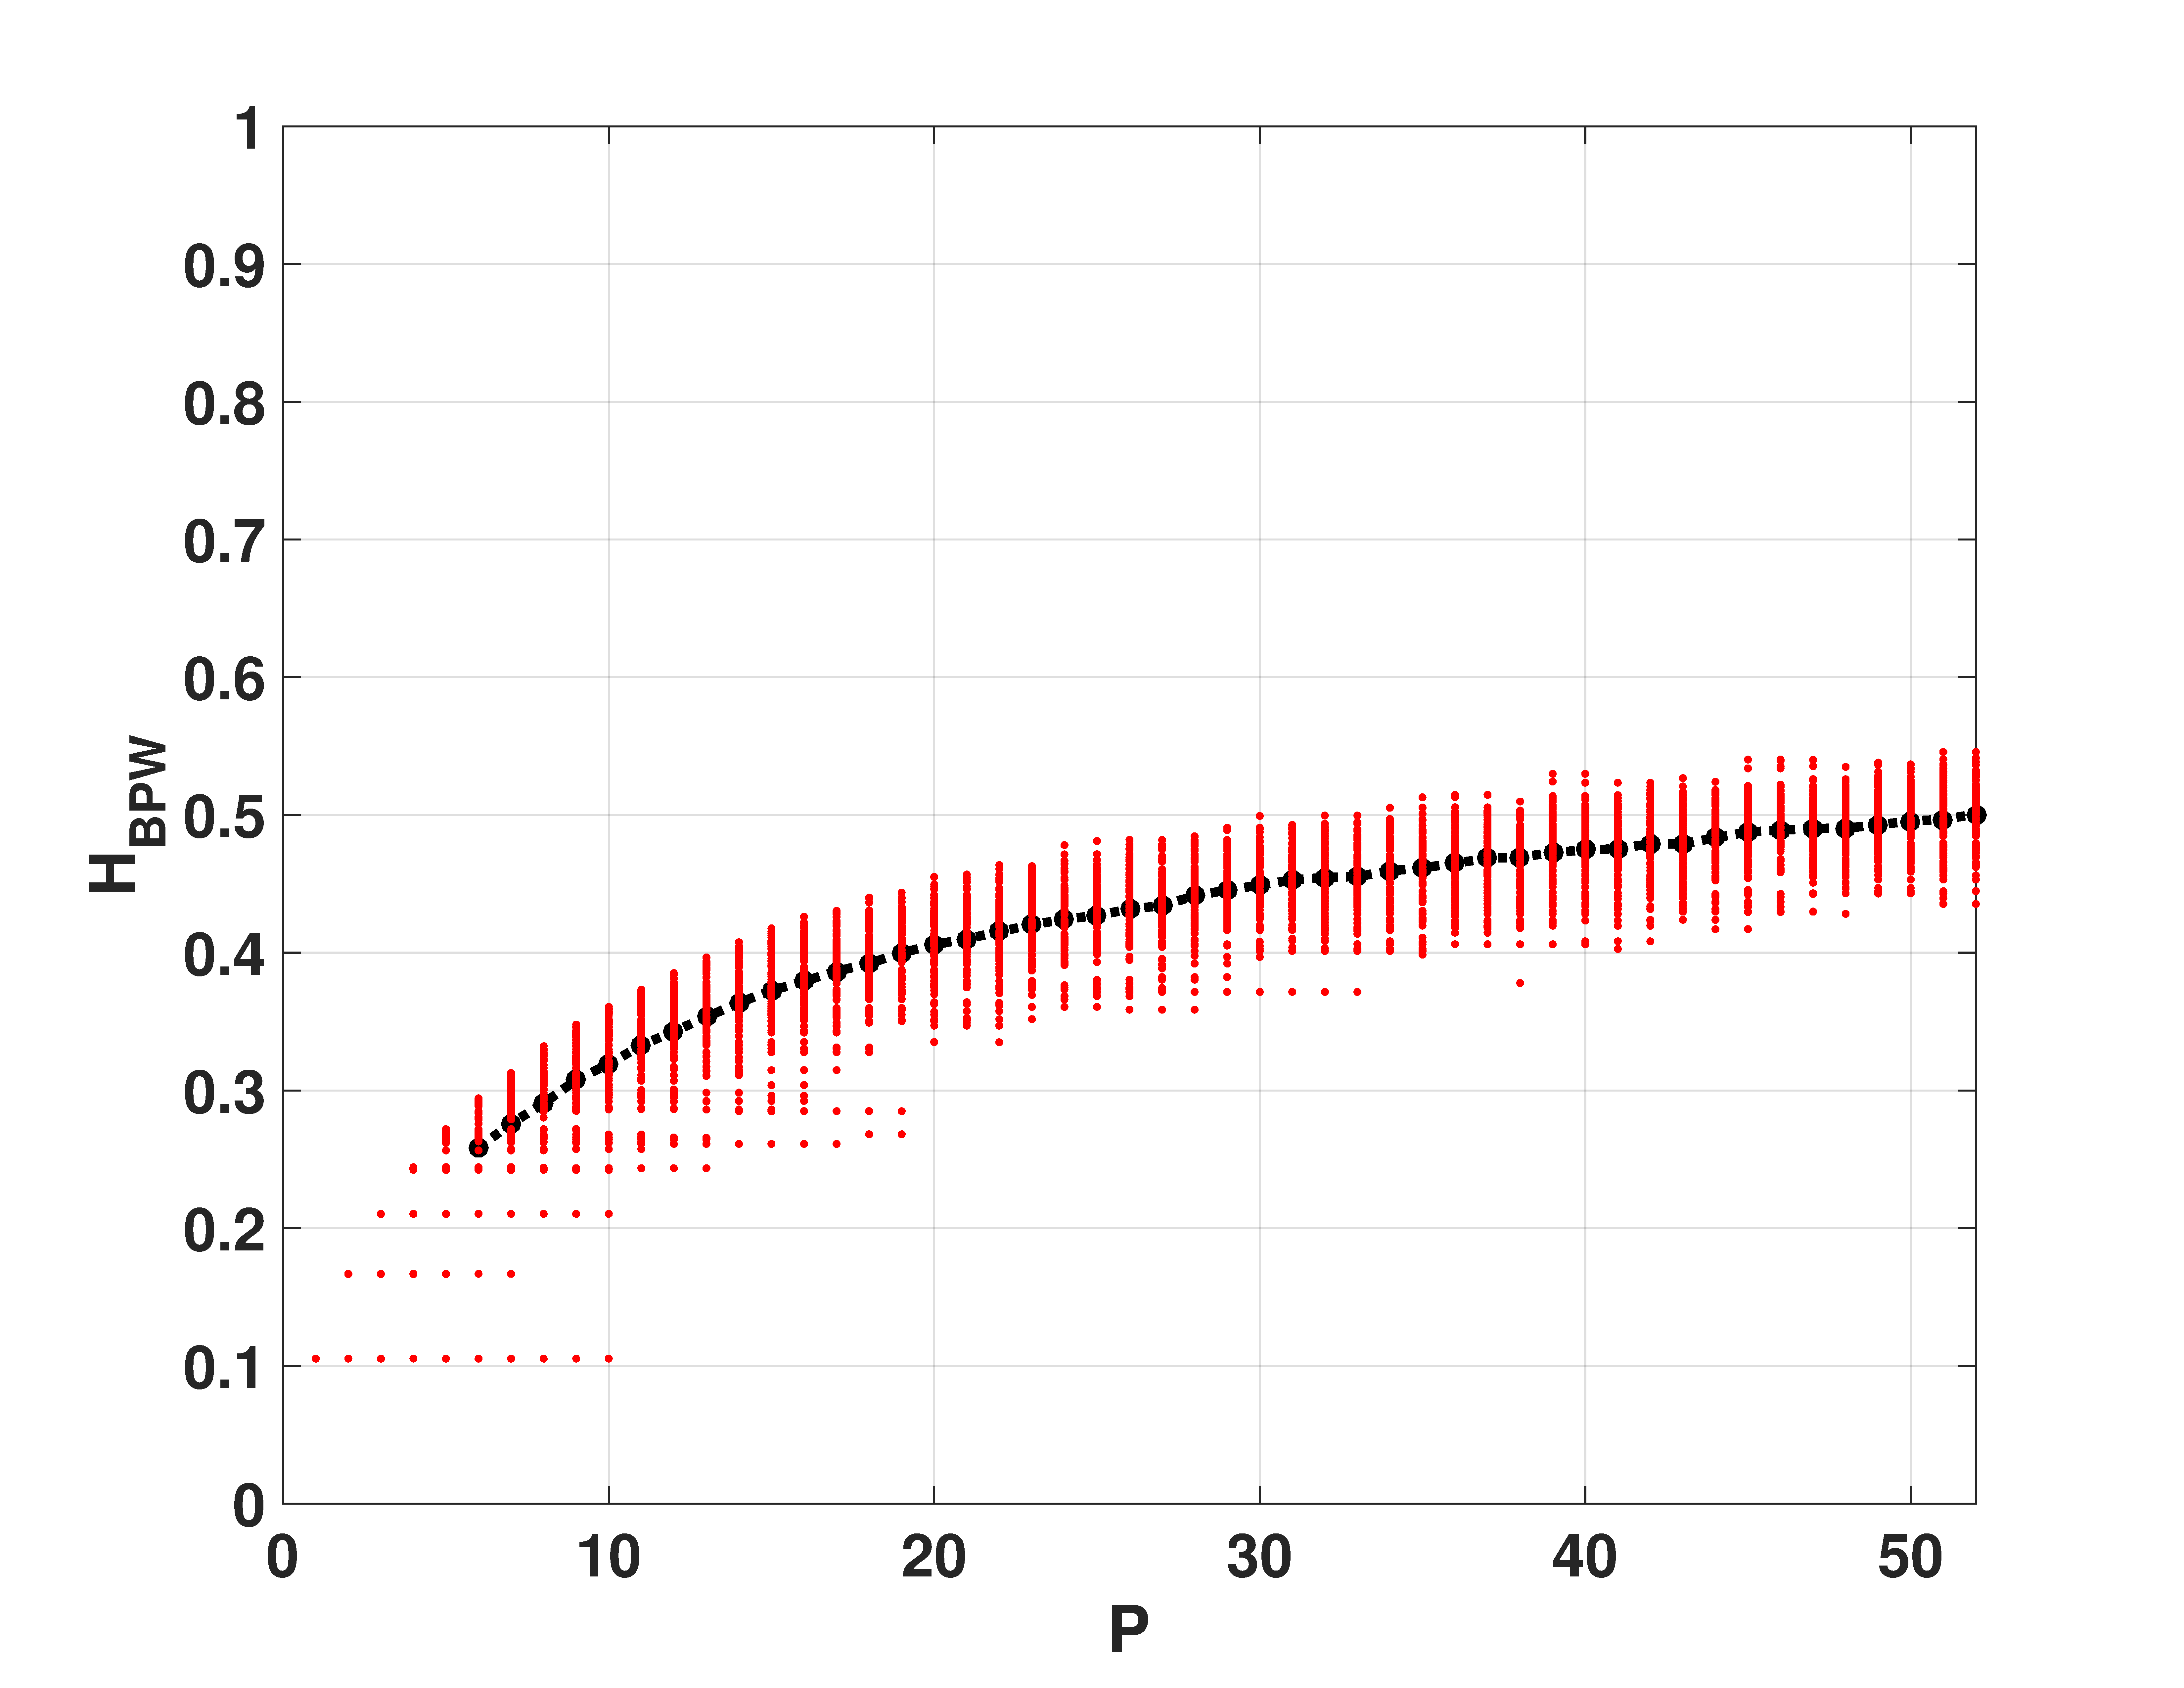
\includegraphics[width=.32\textwidth]{Hbpw_TentB2}
	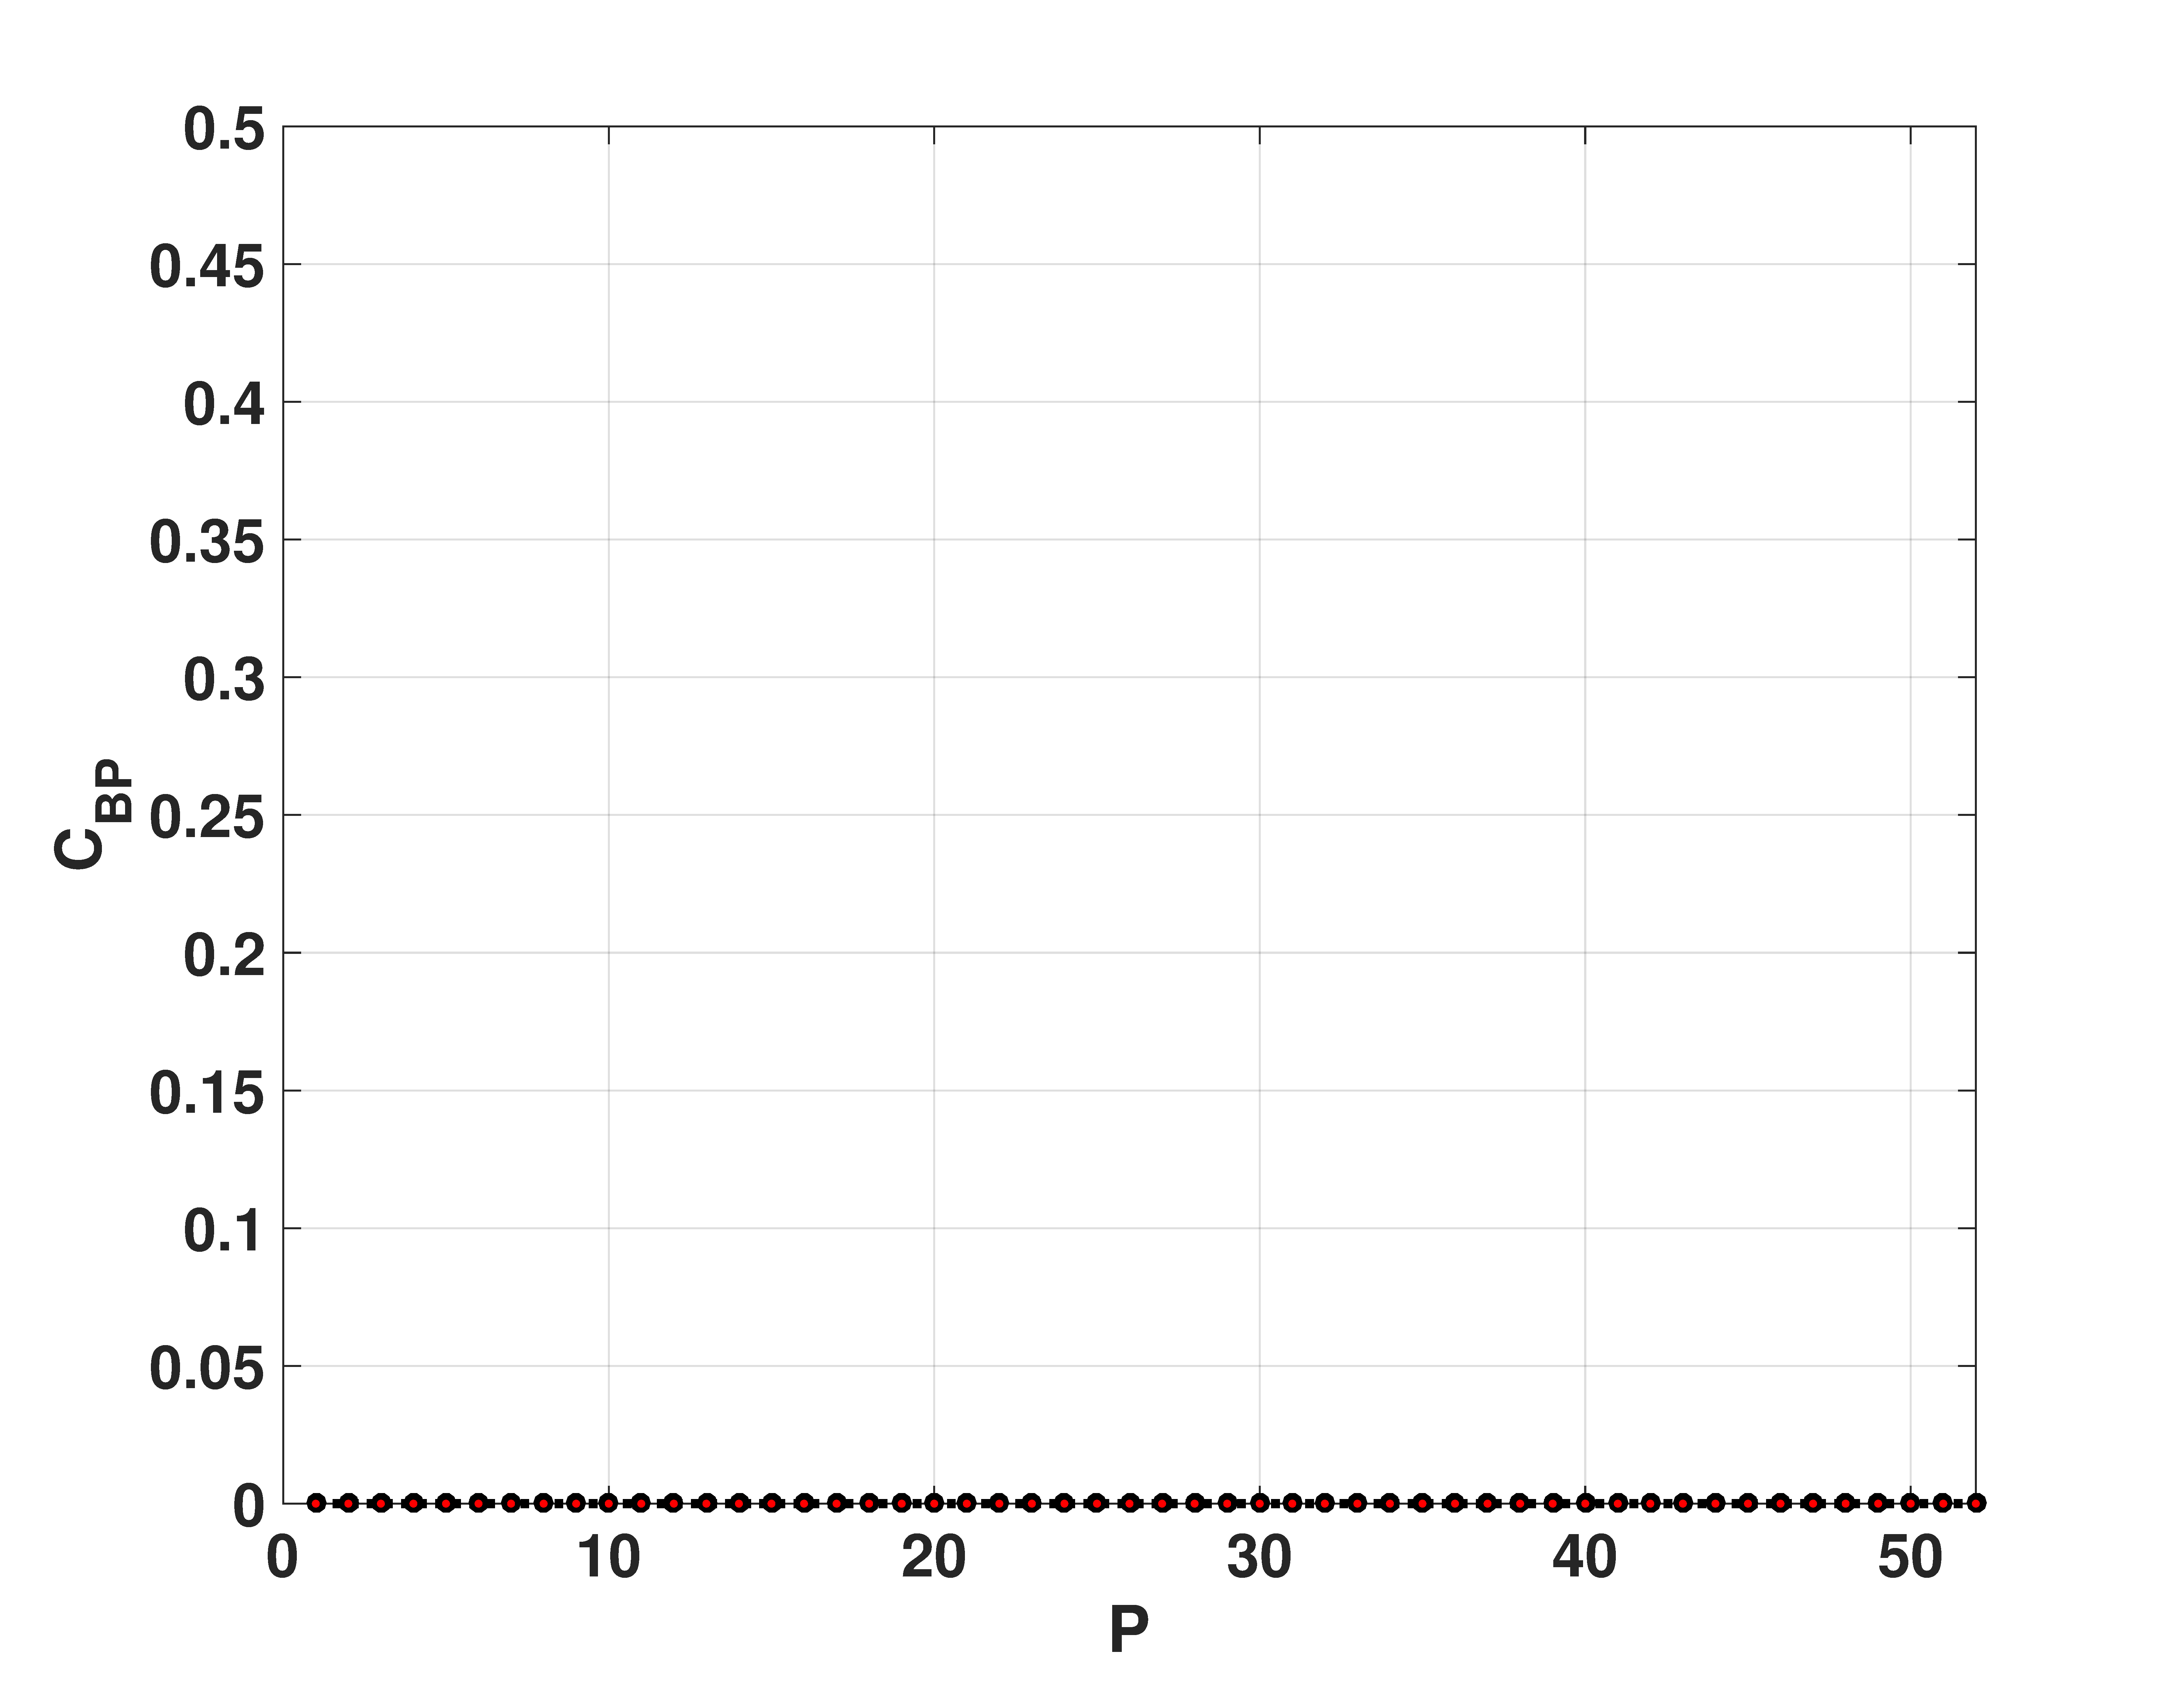
\includegraphics[width=.32\textwidth]{Cbp_TentB2}
	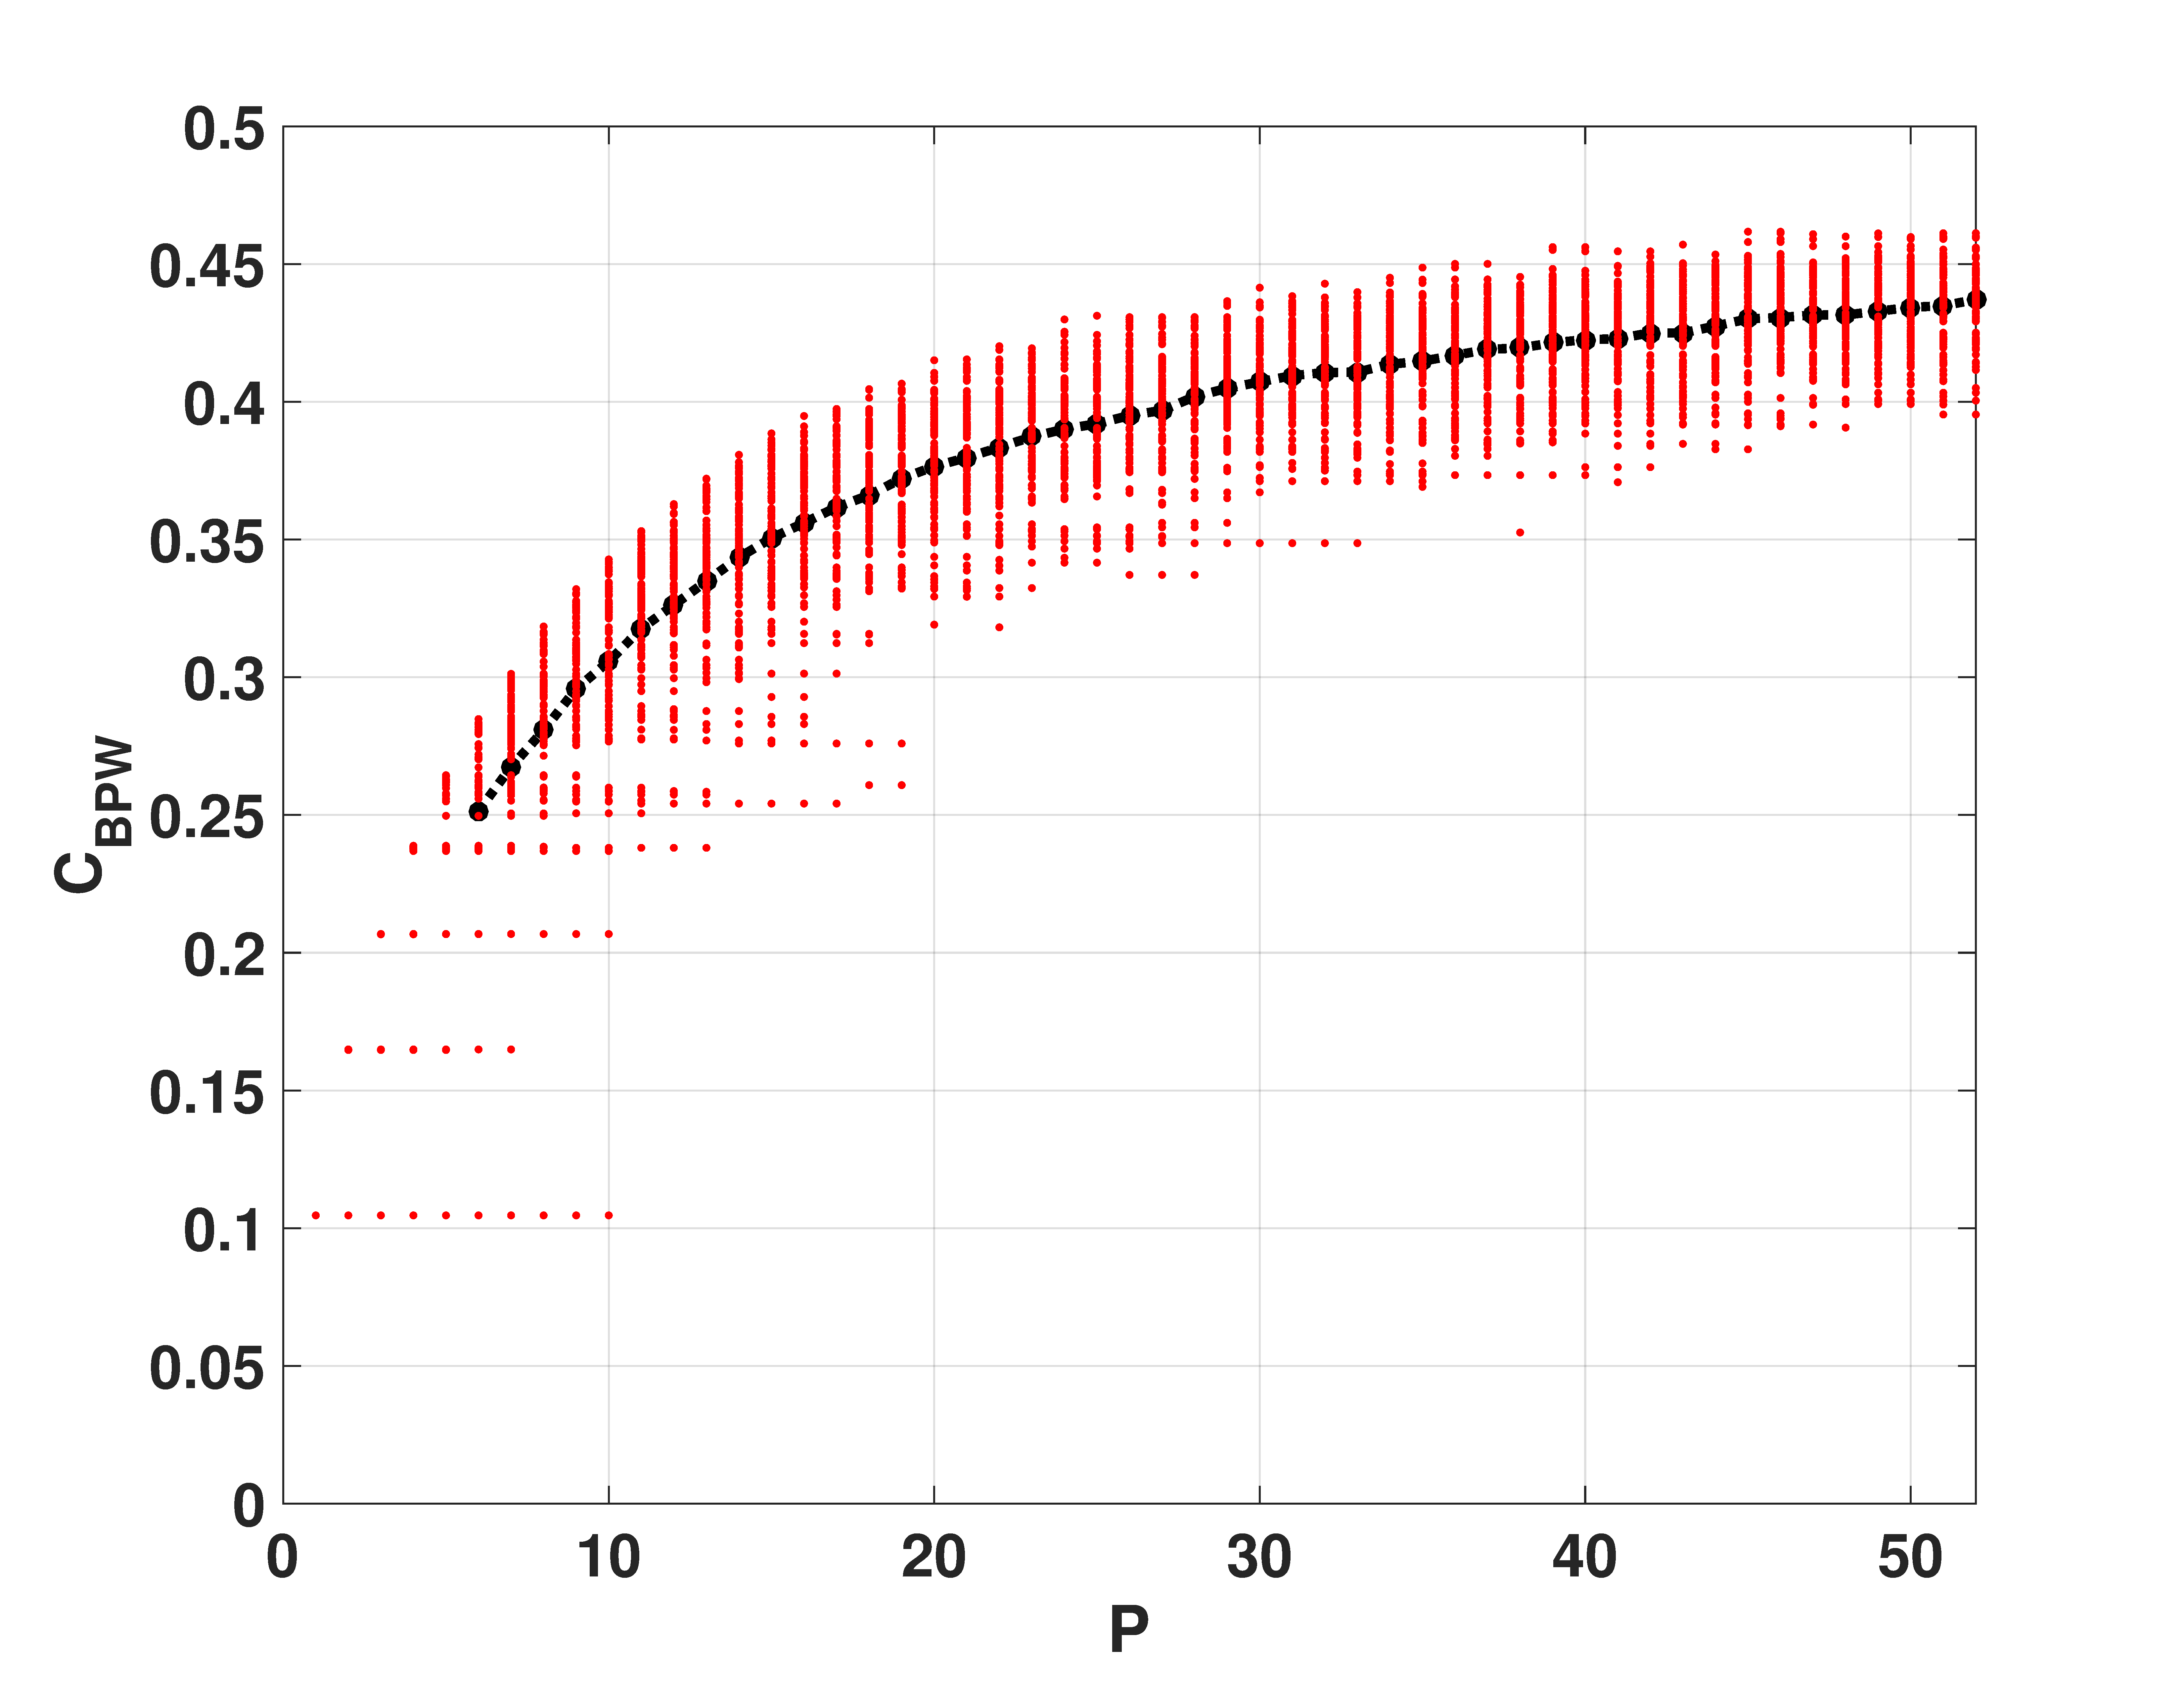
\includegraphics[width=.32\textwidth]{Cbpw_TentB2}
	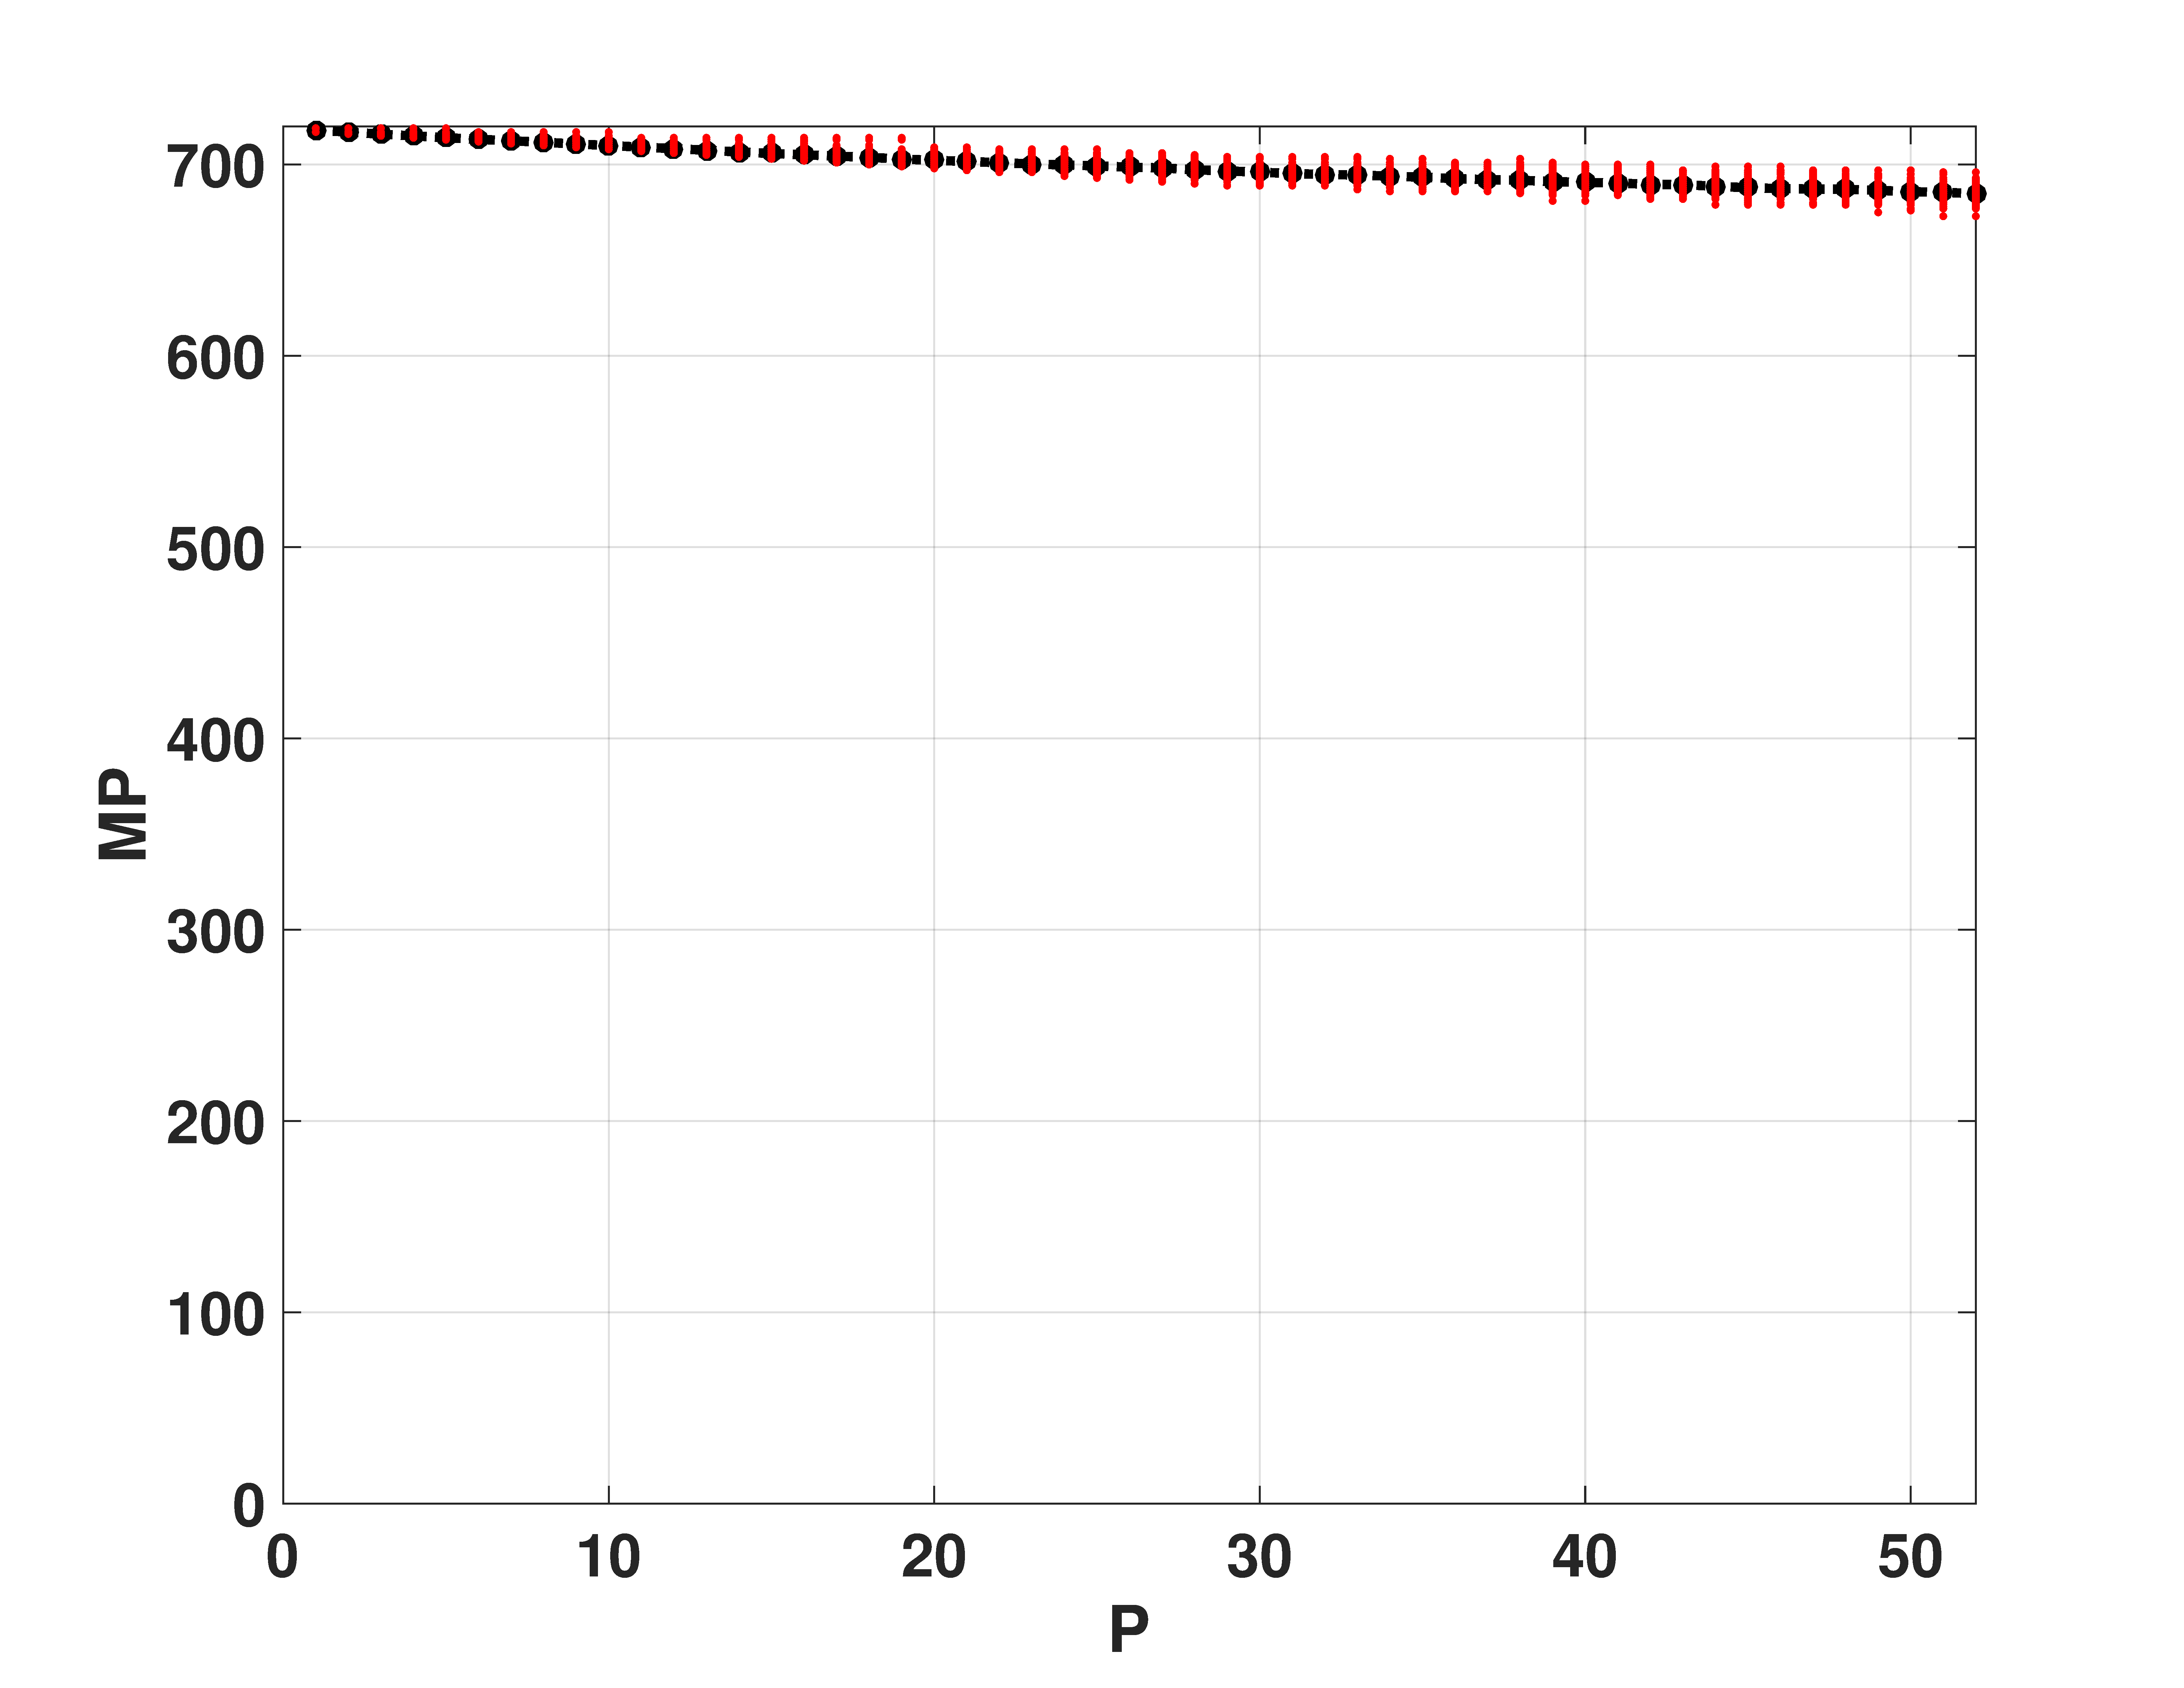
\includegraphics[width=.32\textwidth]{MP_TentB2}
	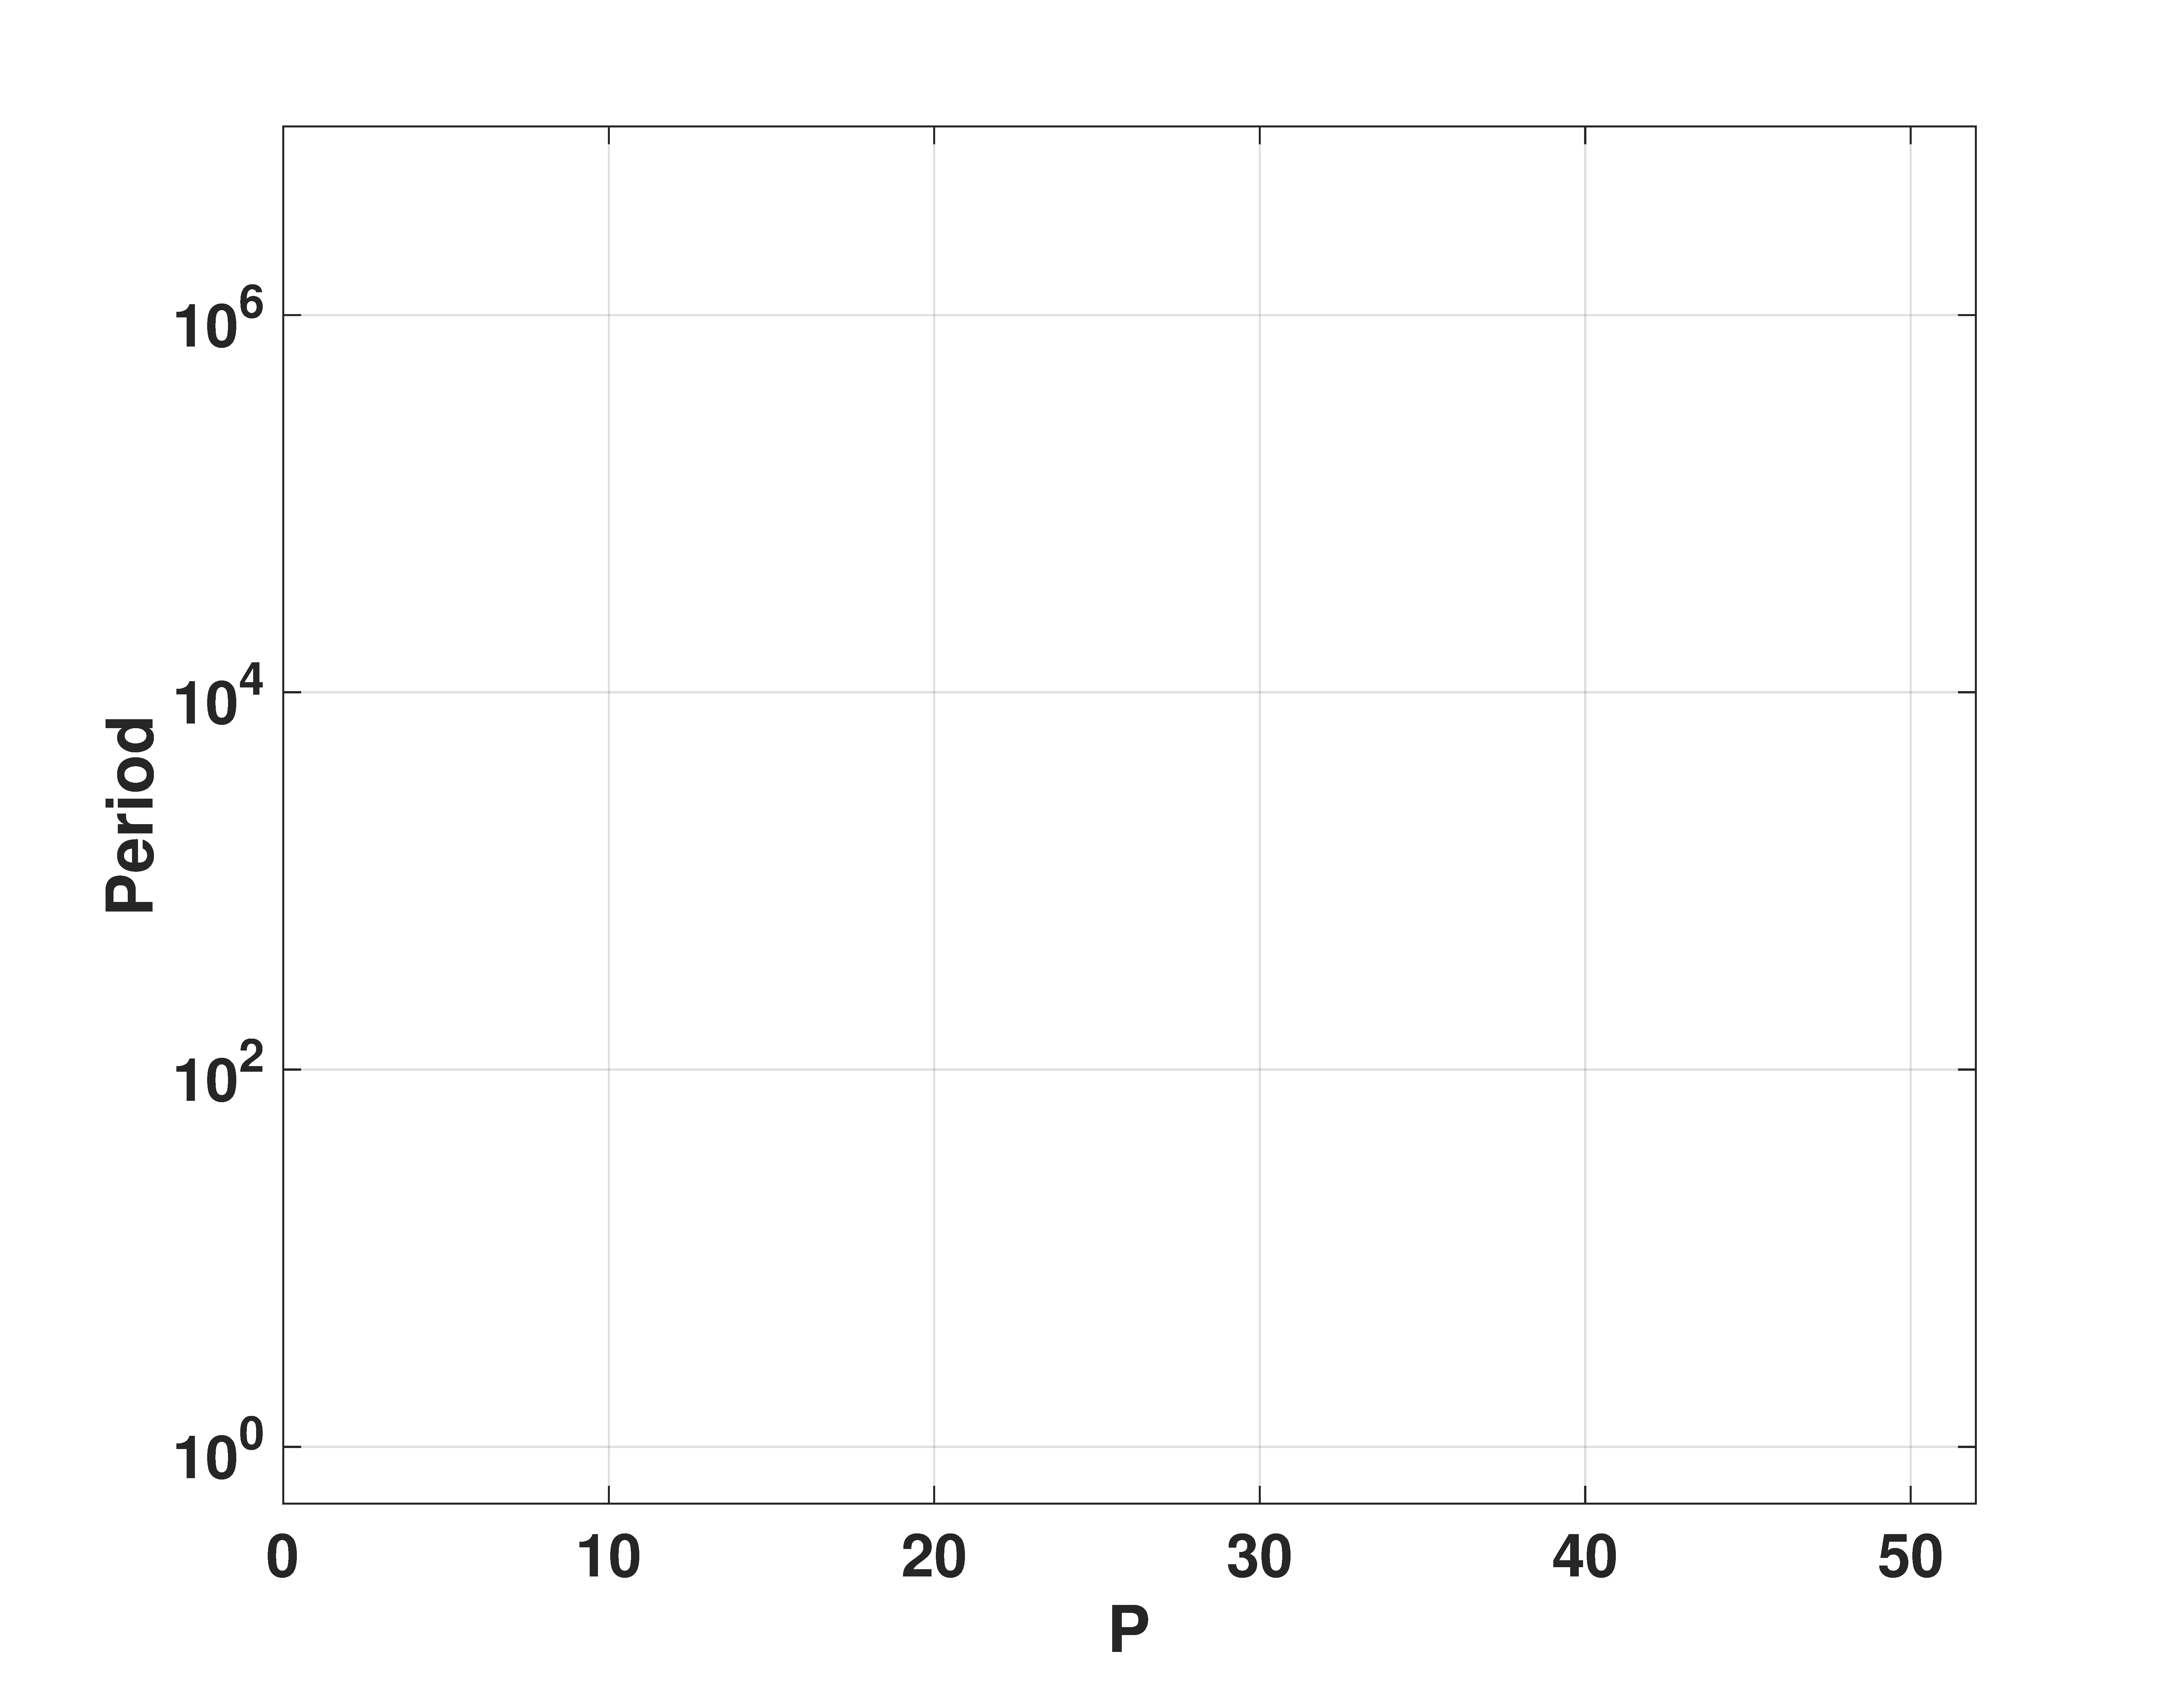
\includegraphics[width=.32\textwidth]{Period_TentB2}
	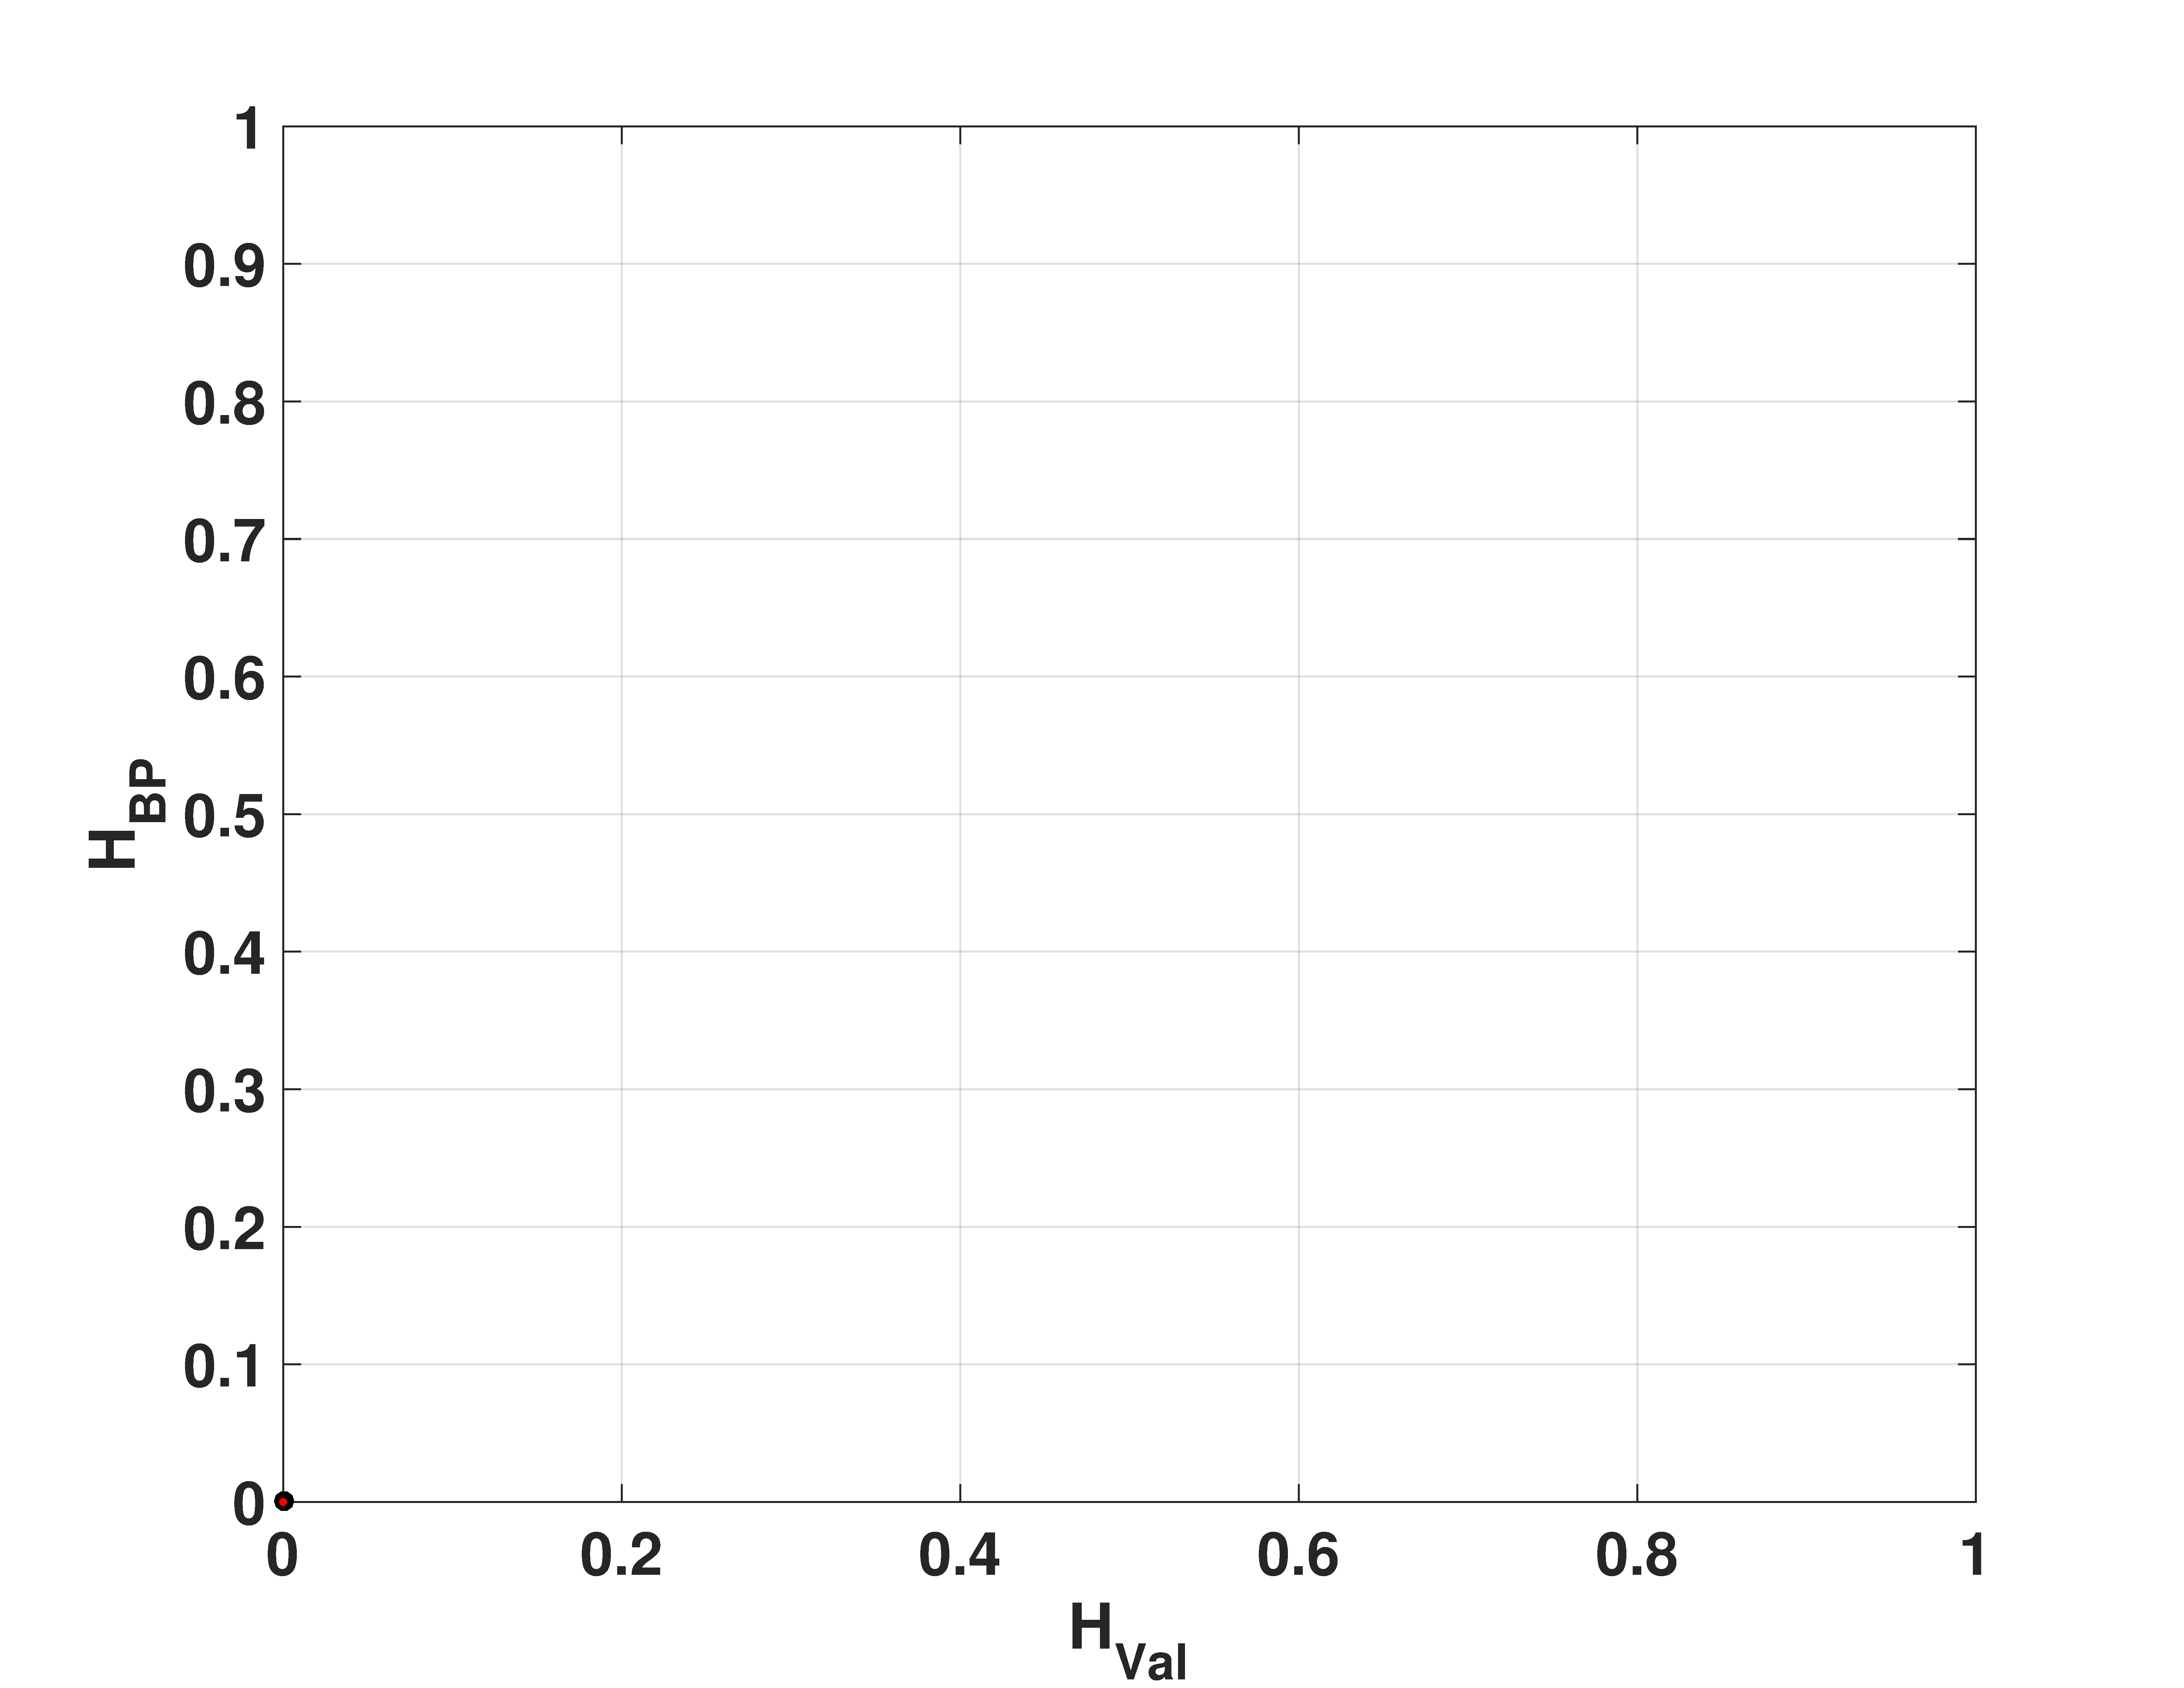
\includegraphics[width=.32\textwidth]{HbpHval_TentB2}
	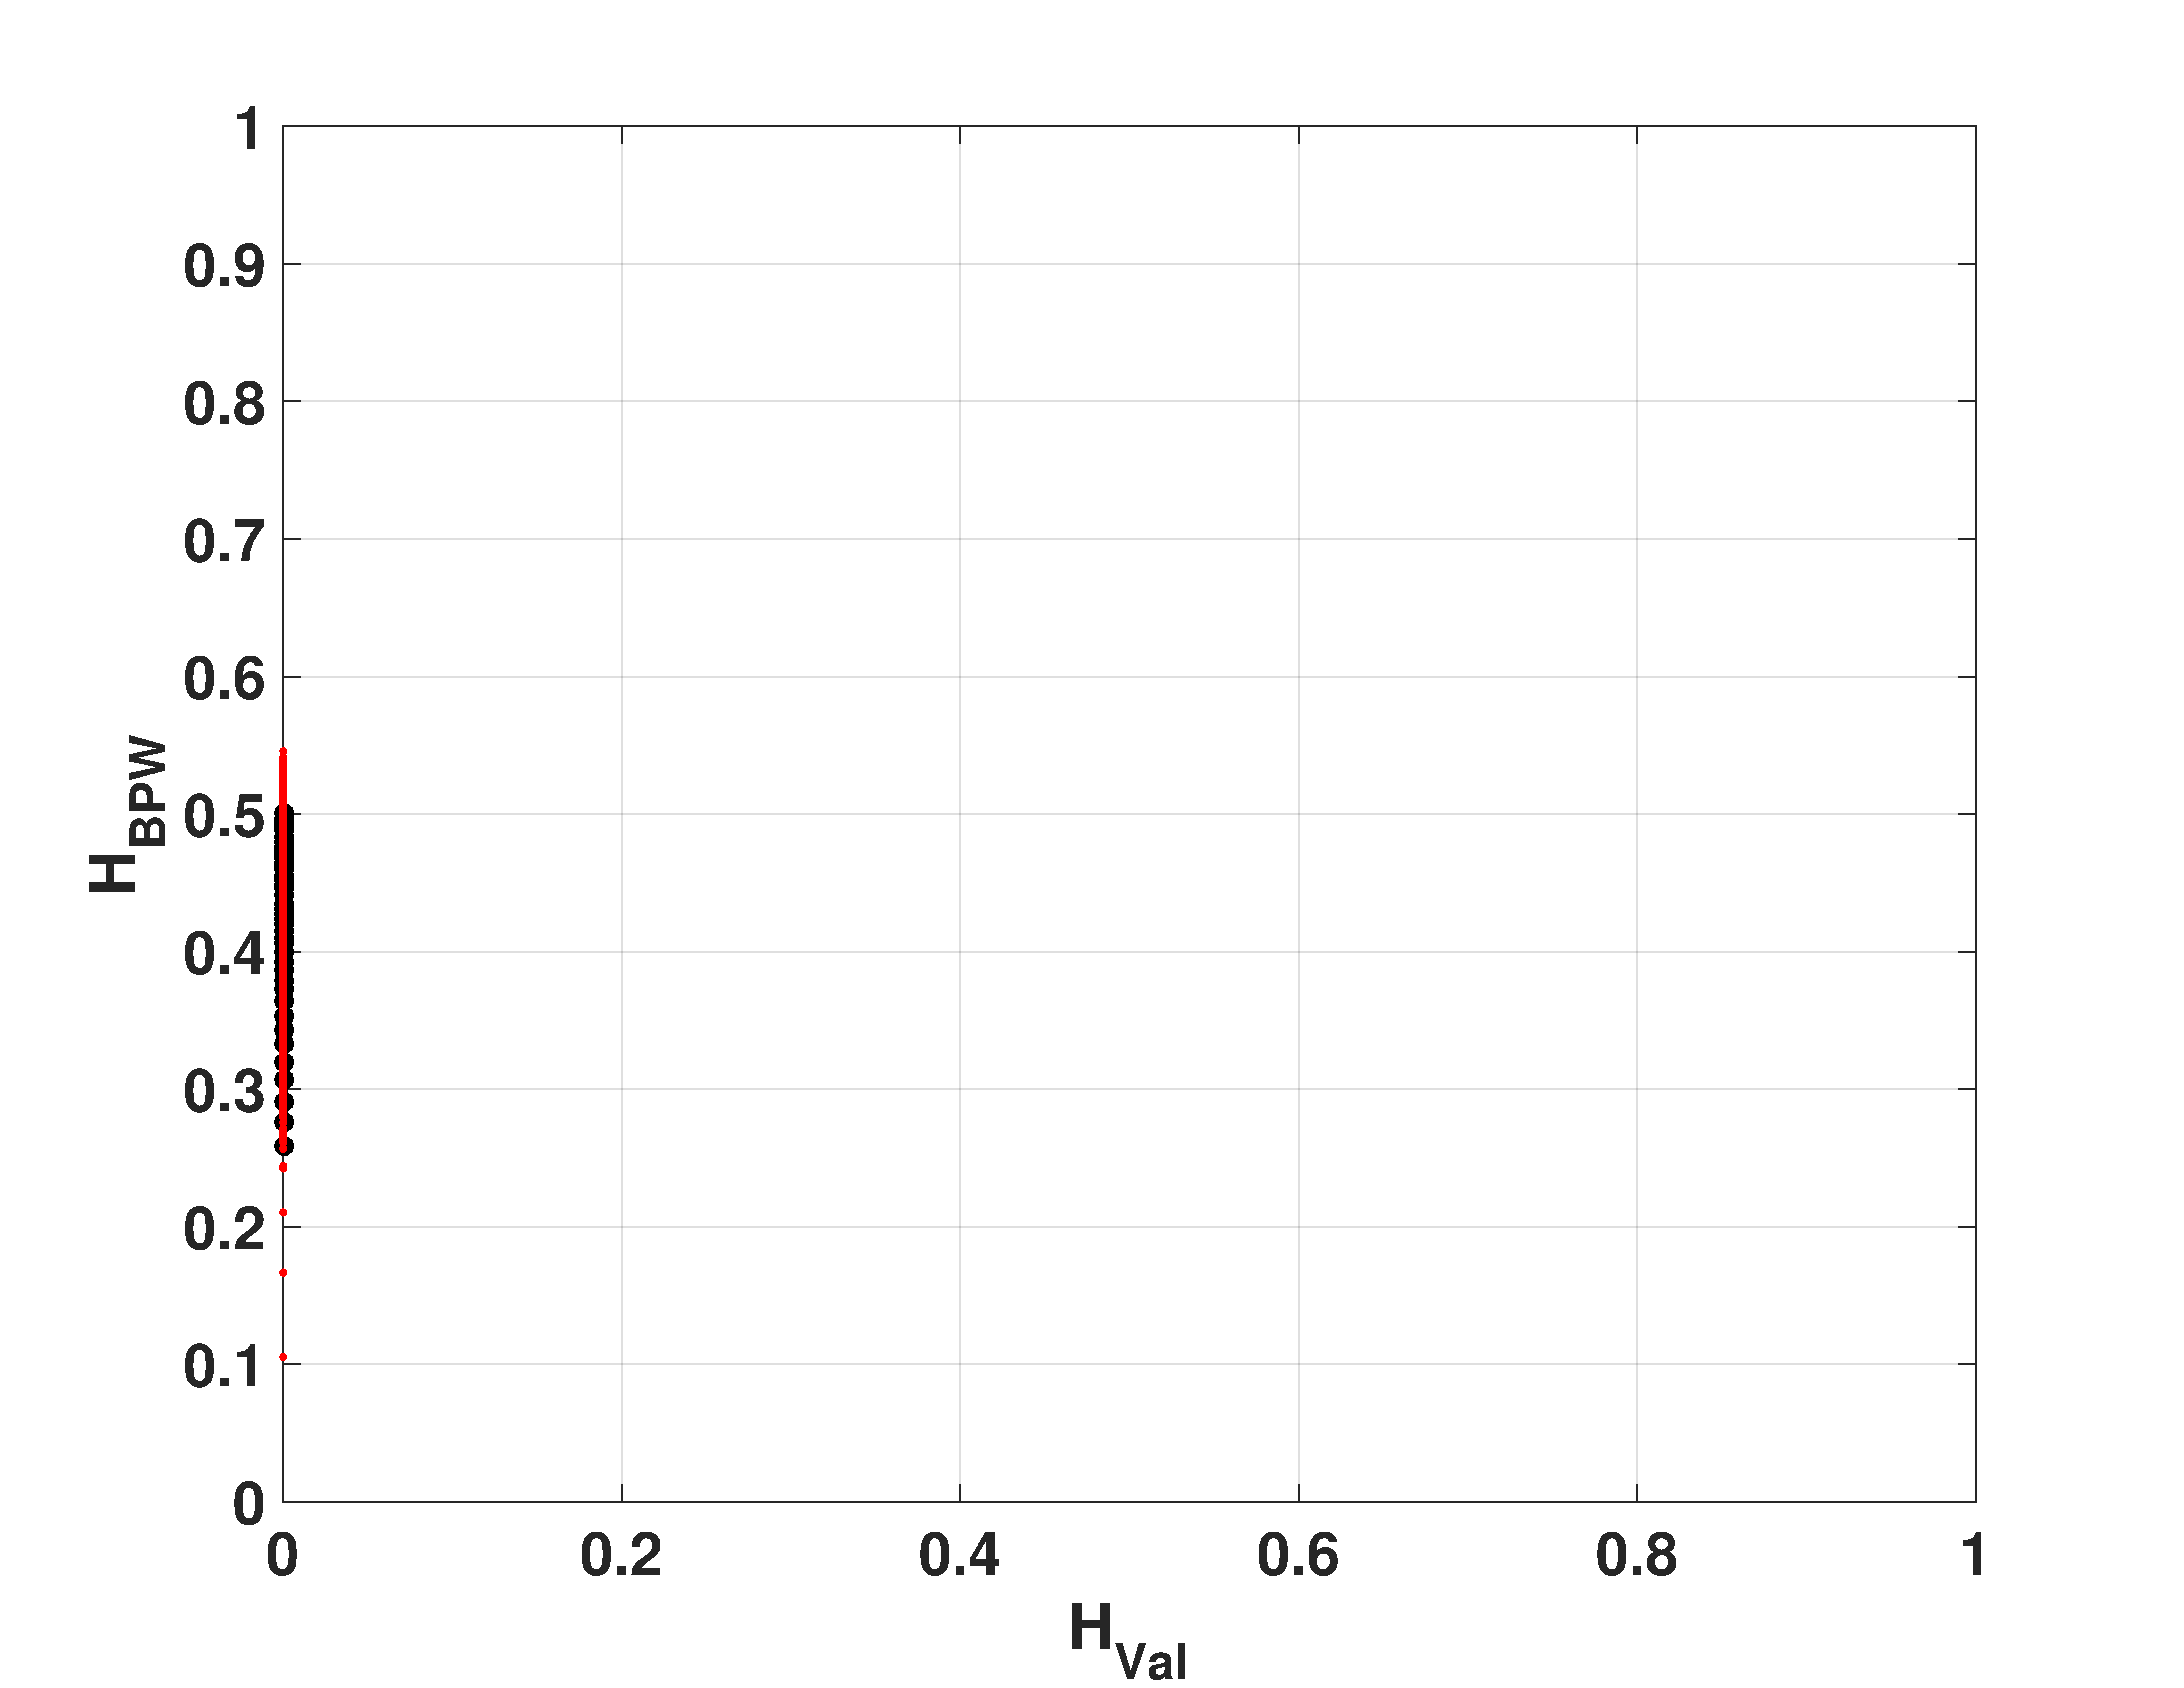
\includegraphics[width=.32\textwidth]{HbpwHval_TentB2}
	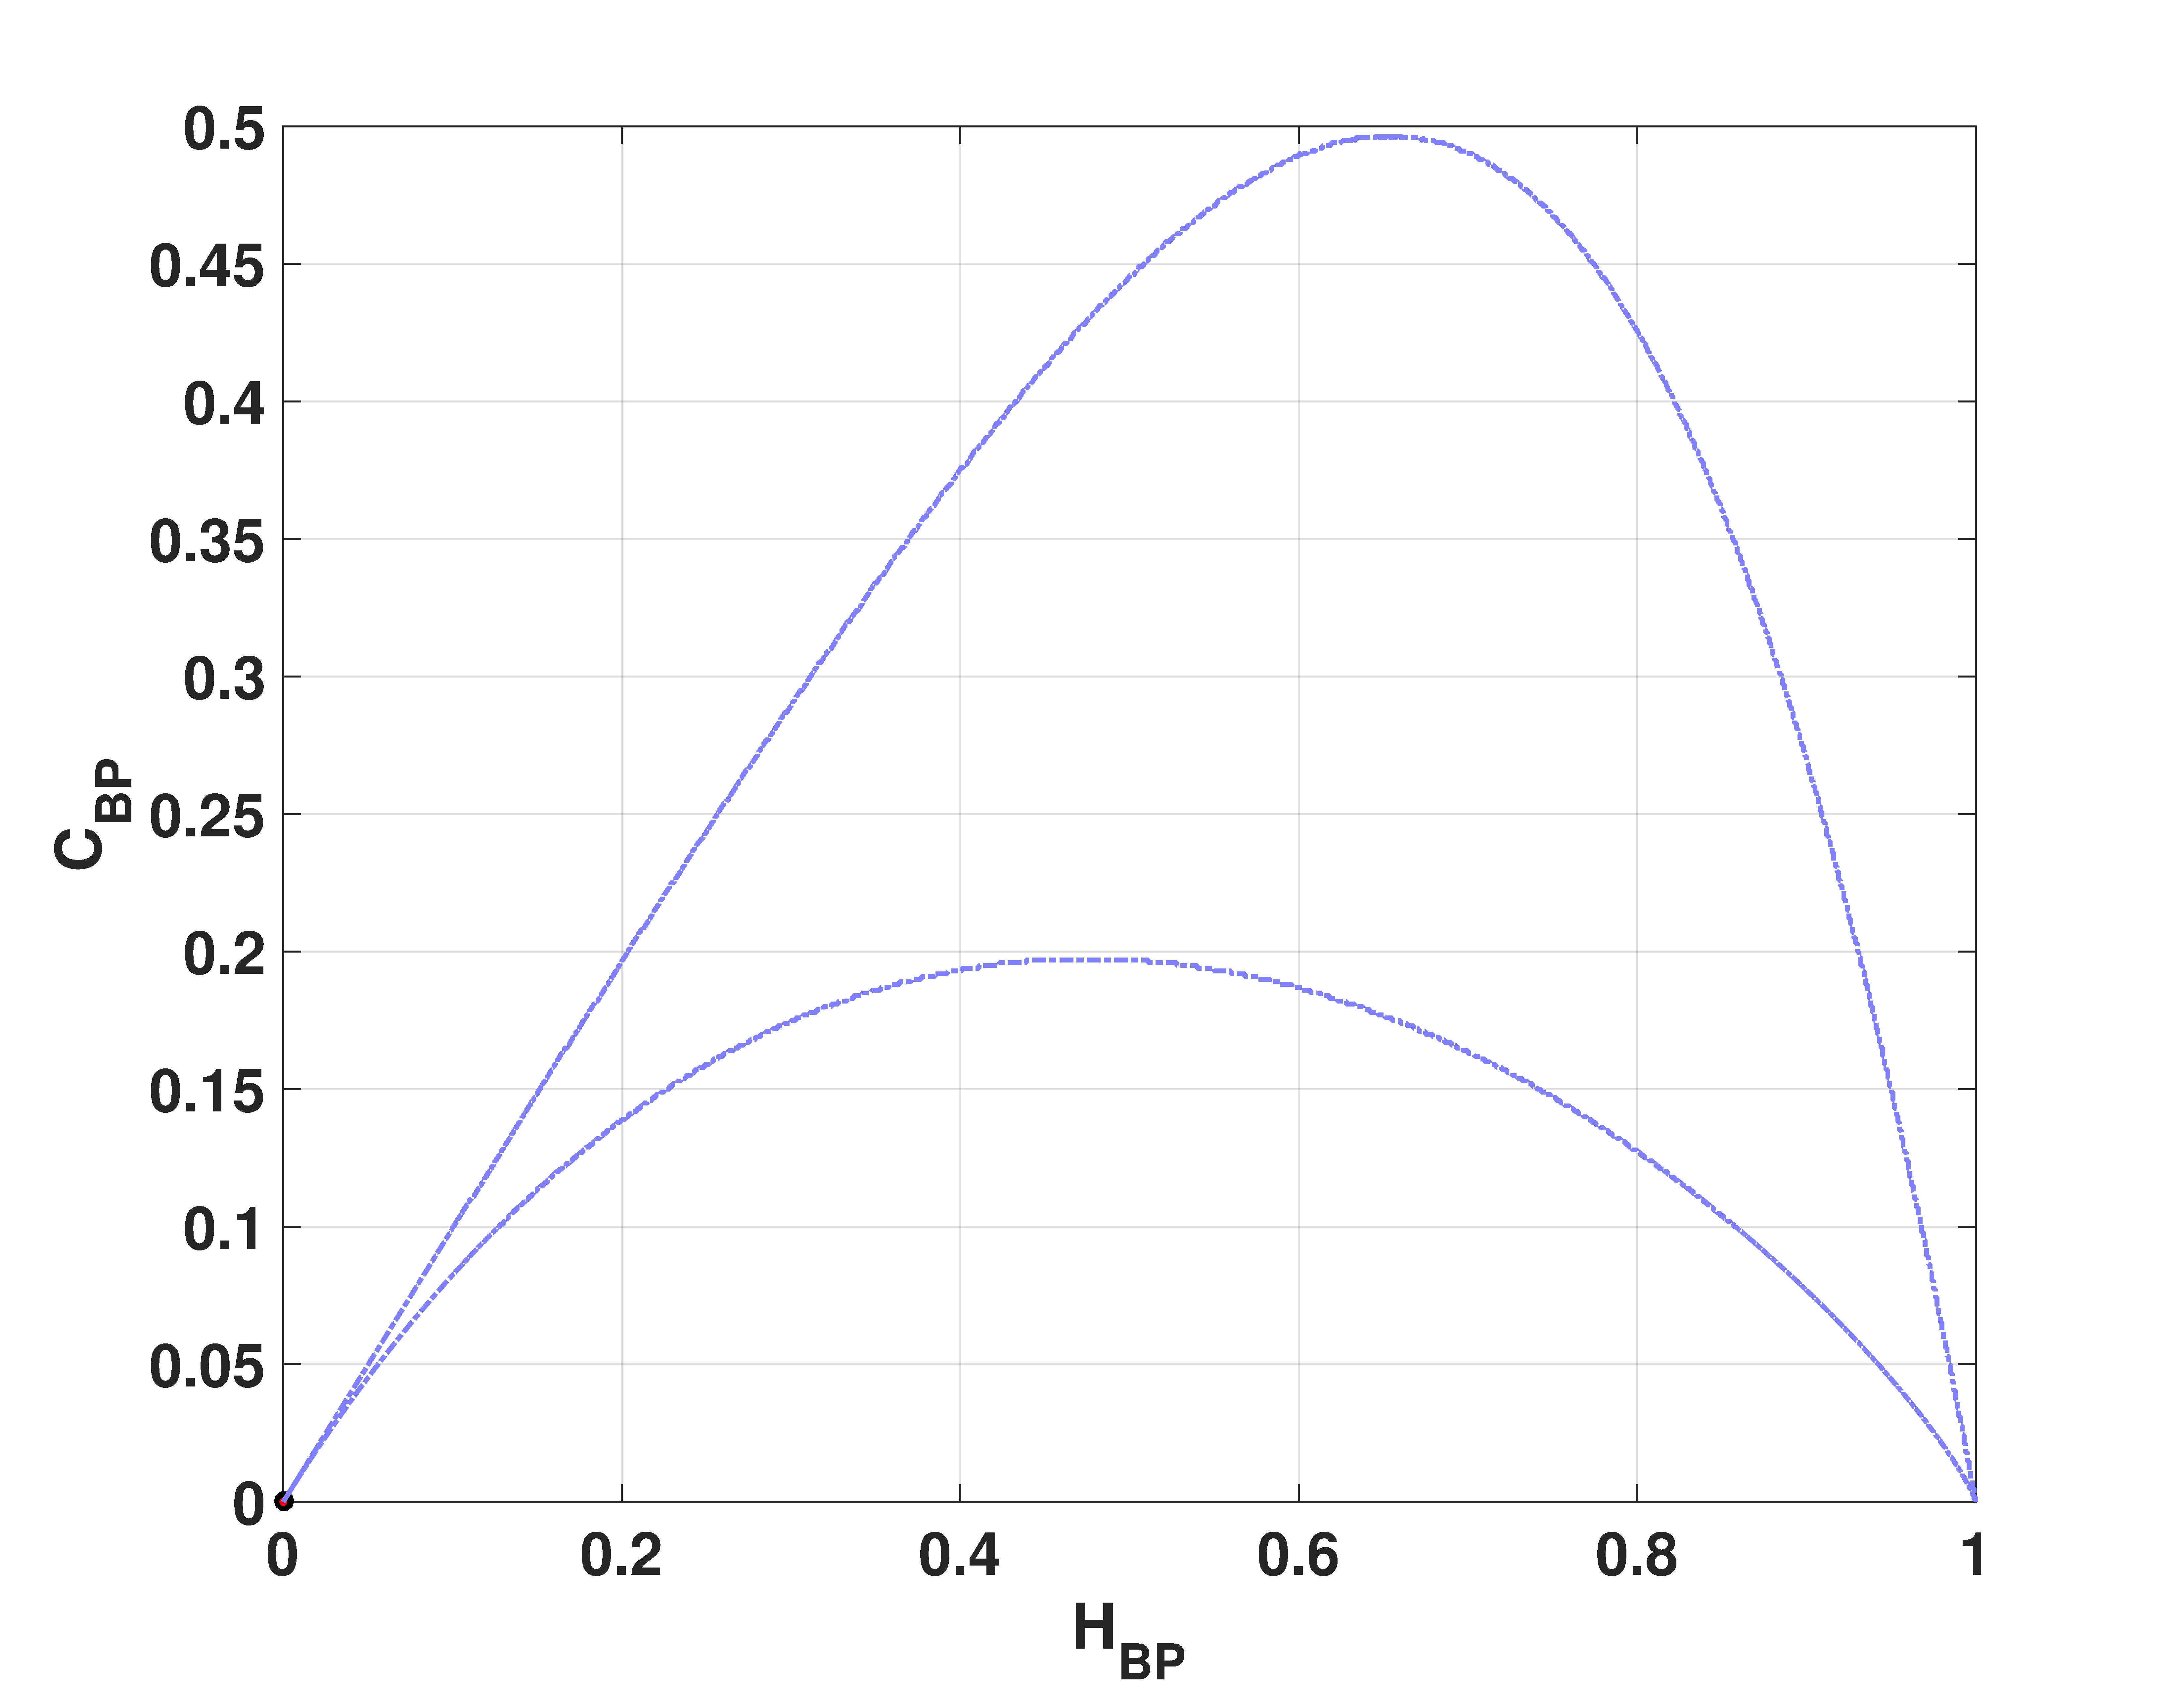
\includegraphics[width=.32\textwidth]{CbpHbp_TentB2}
	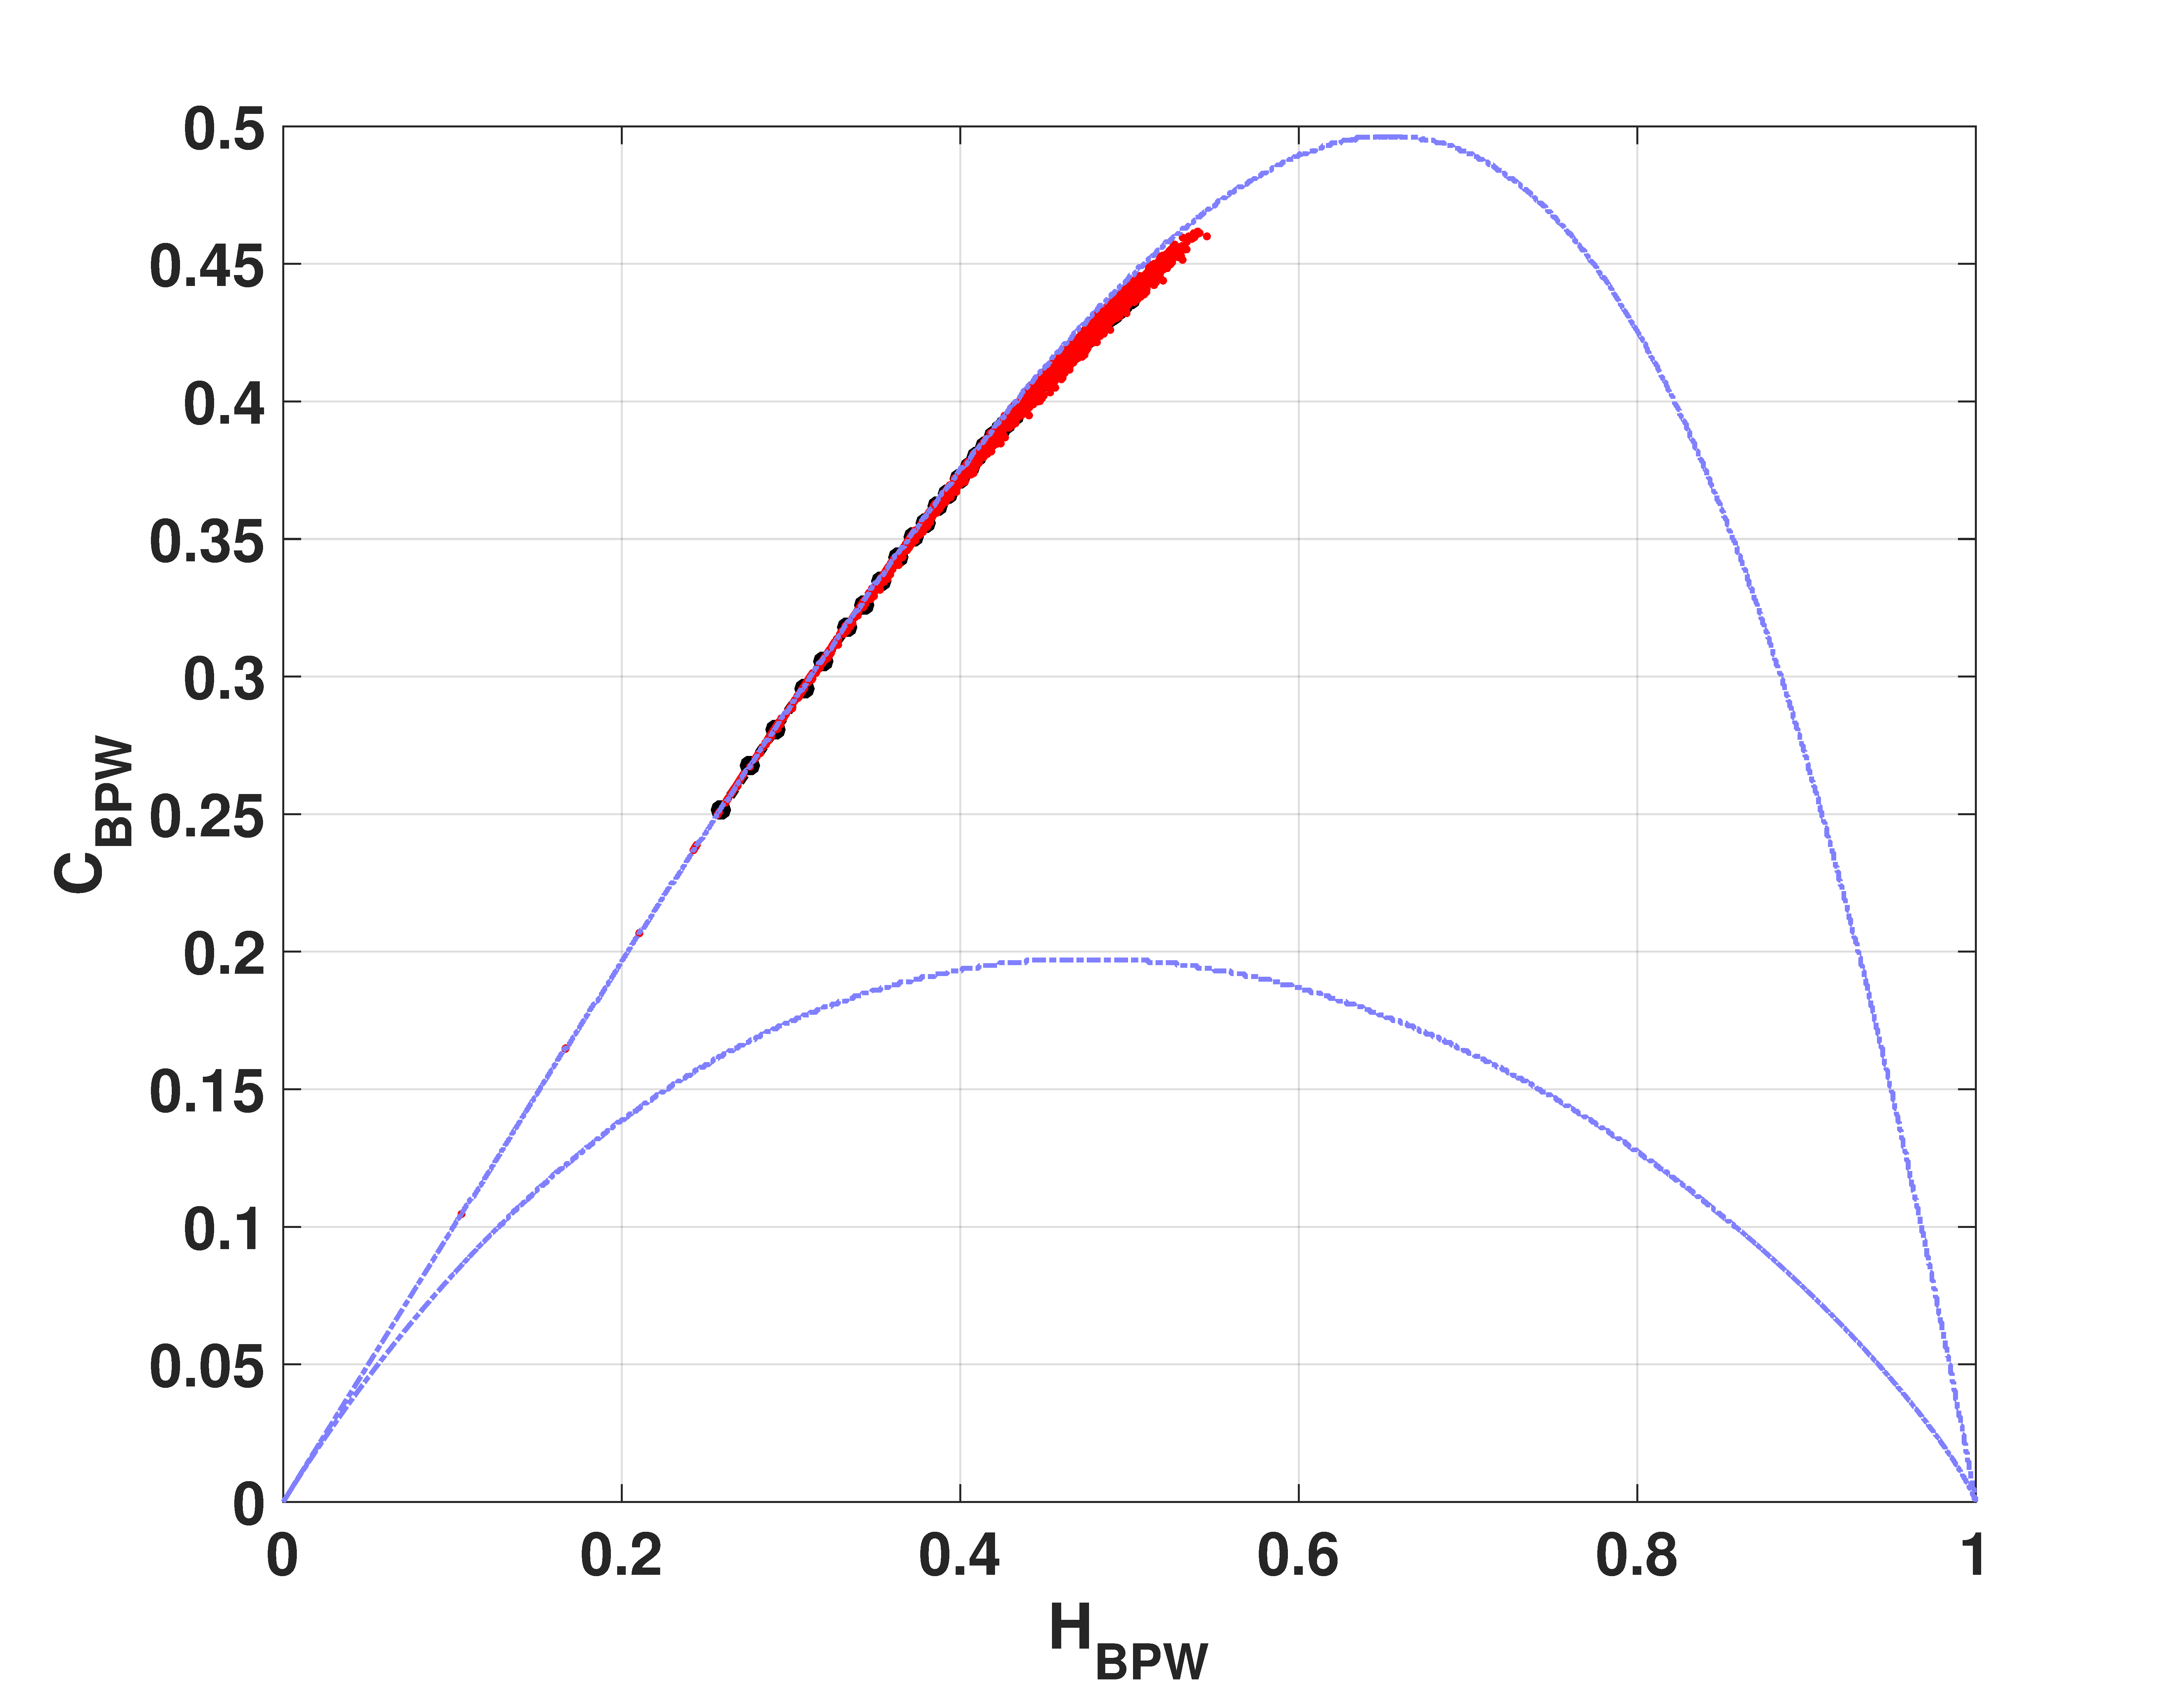
\includegraphics[width=.32\textwidth]{CbpwHbpw_TentB2}
	\caption{Statistical properties of the SWITCH map using binary representation: (a) $H_{hist}$ vs $P$ (b) $H_{BP}$ vs $P$ (c) $C_{BP}$ vs $P$ (d) Number of missing ordering patterns $MP$ vs $P$. In Figures (a) to (d) dashed line correspond to floating point numbers. (e) representation in the $H_{hist},H_{BP}$ plane in the the binary numerical system.  The star represents the state for floating points numbers. (f) representation in the $H_{BP},C_{BP}$ plane.  The star represents the state for floating points numbers. (The star represents the state for floating points numbers). } \label{fig:seqbin}
\end{figure}

%%%%%%%%%%%%%%%%%%%%%%%%%%
%%%%%%%%%%%%%%%%%%%%%%%%%%% Fig.7
%\begin{figure}
%	\includegraphics[width=0.3\textwidth]{Hval_parB10}
%	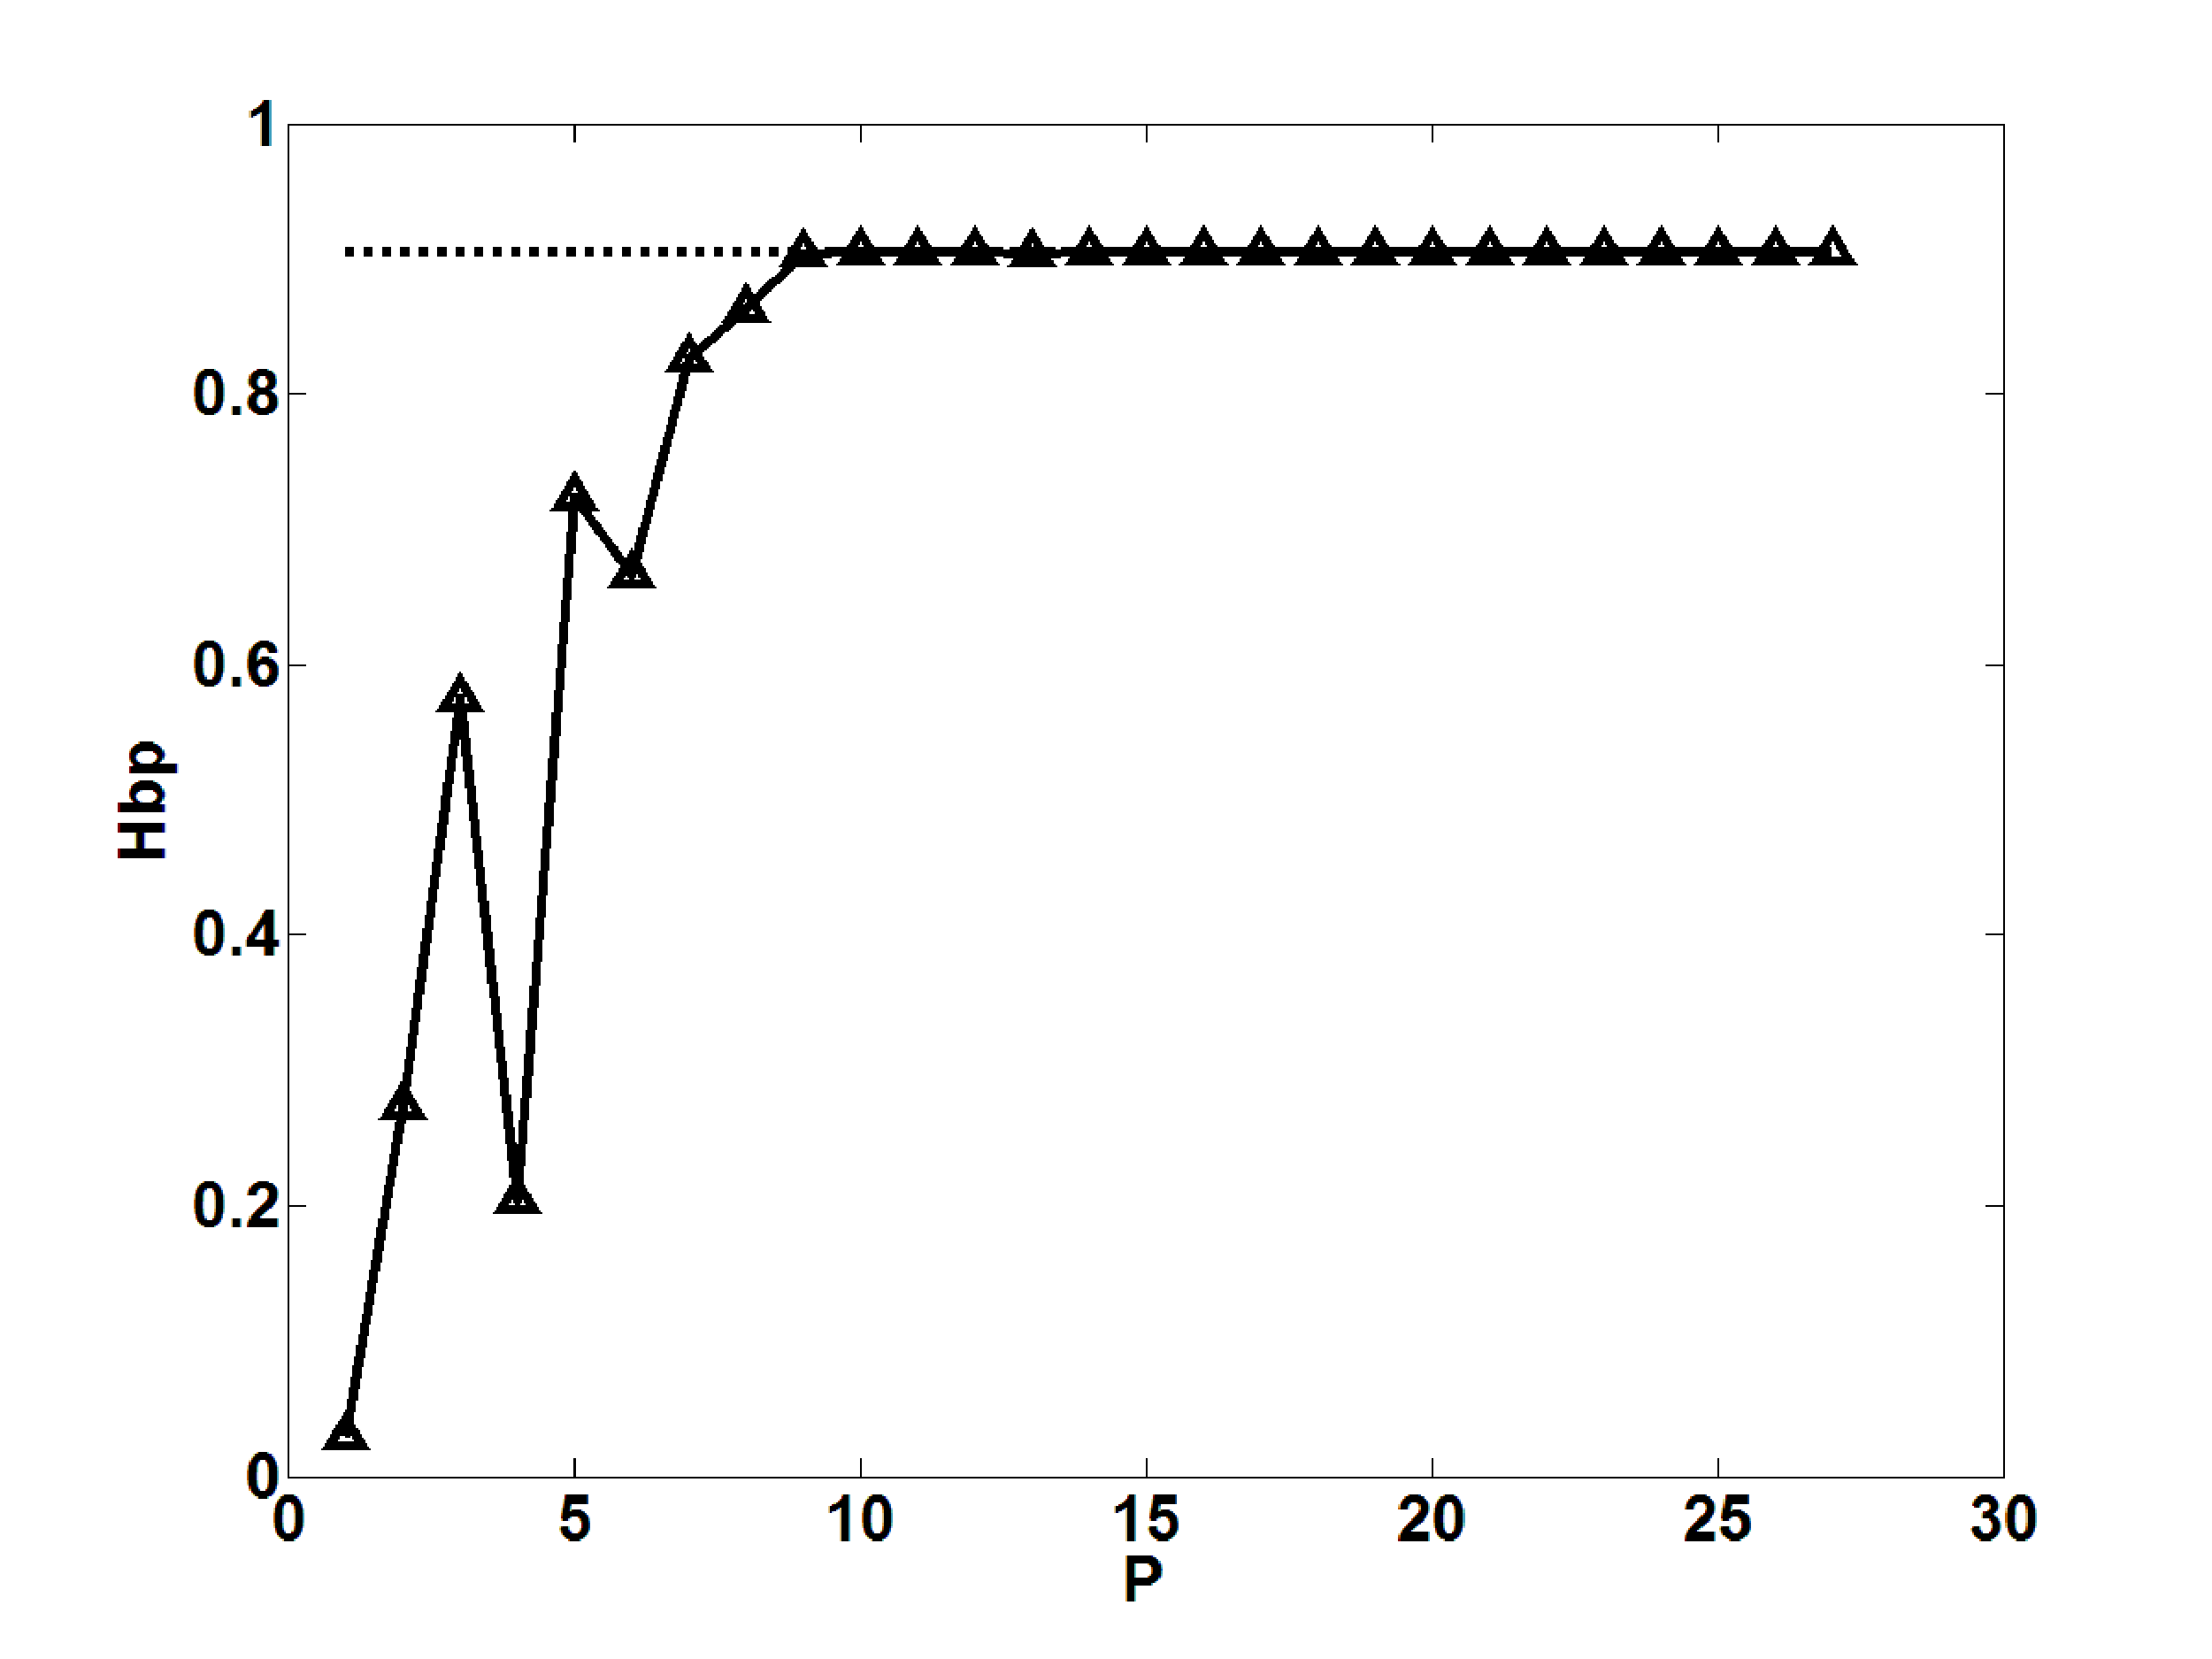
\includegraphics[width=0.3\textwidth]{Hbp_parB10}
%	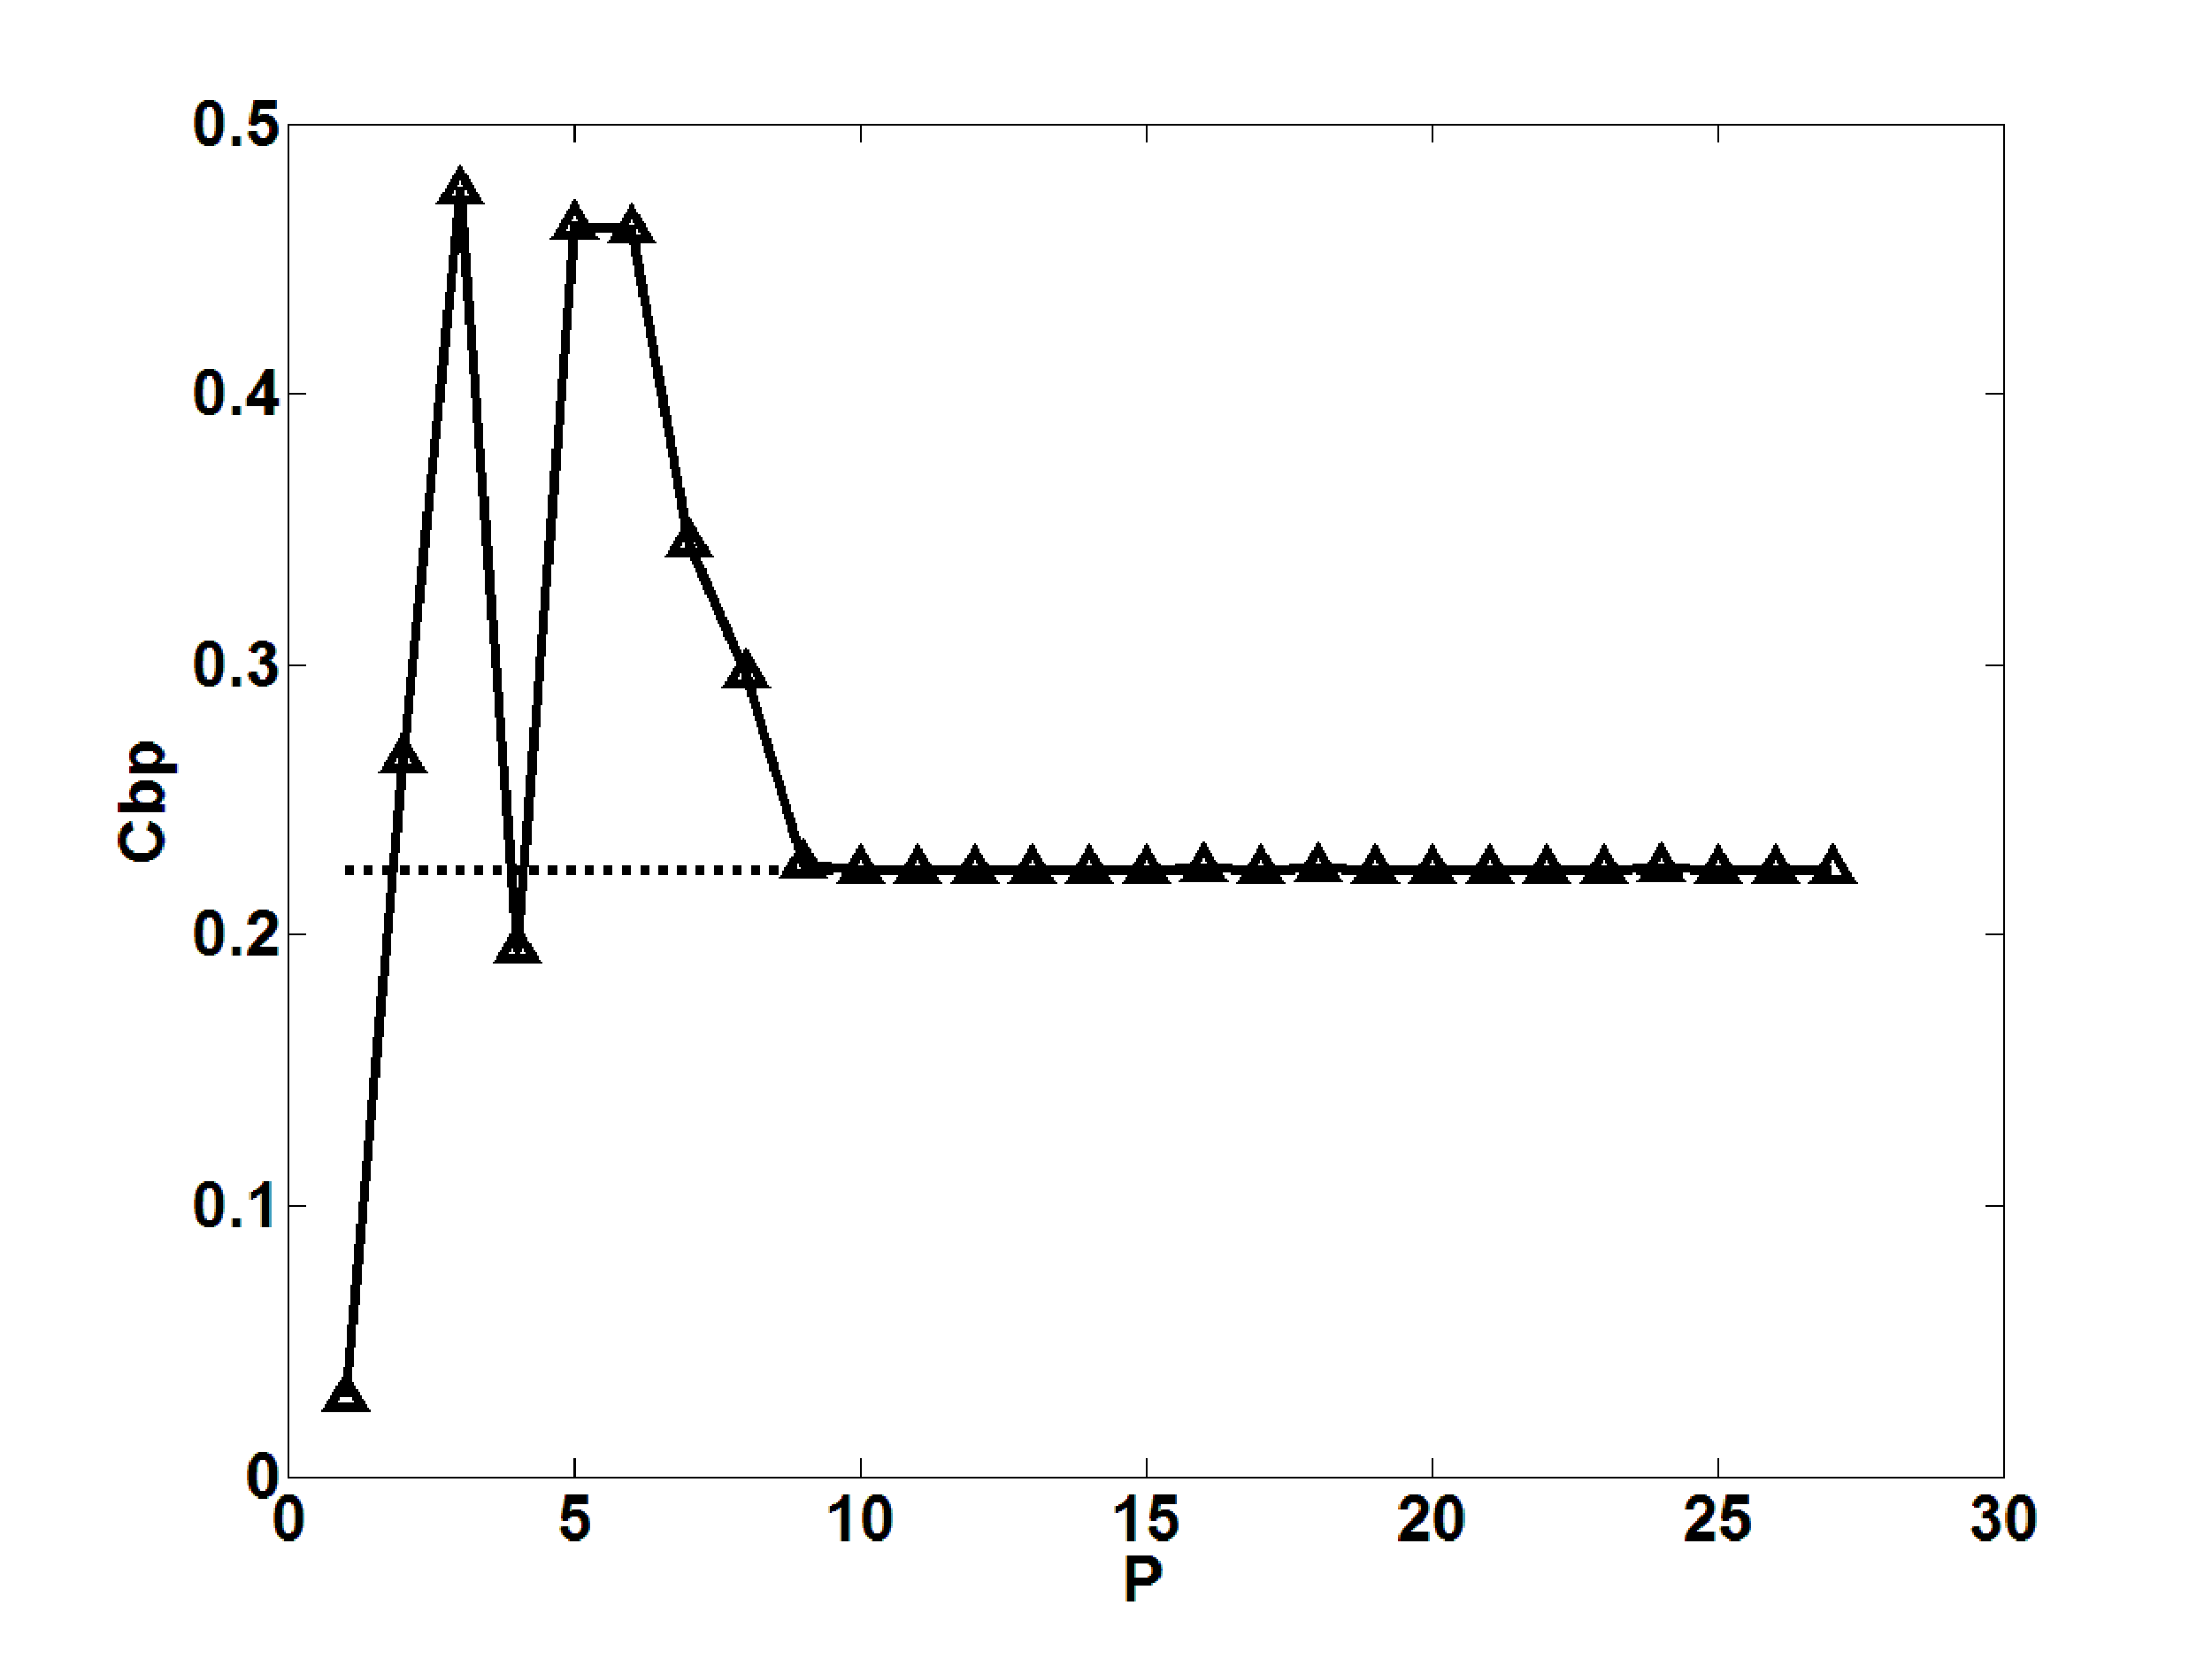
\includegraphics[width=0.3\textwidth]{Cbp_parB10}
%	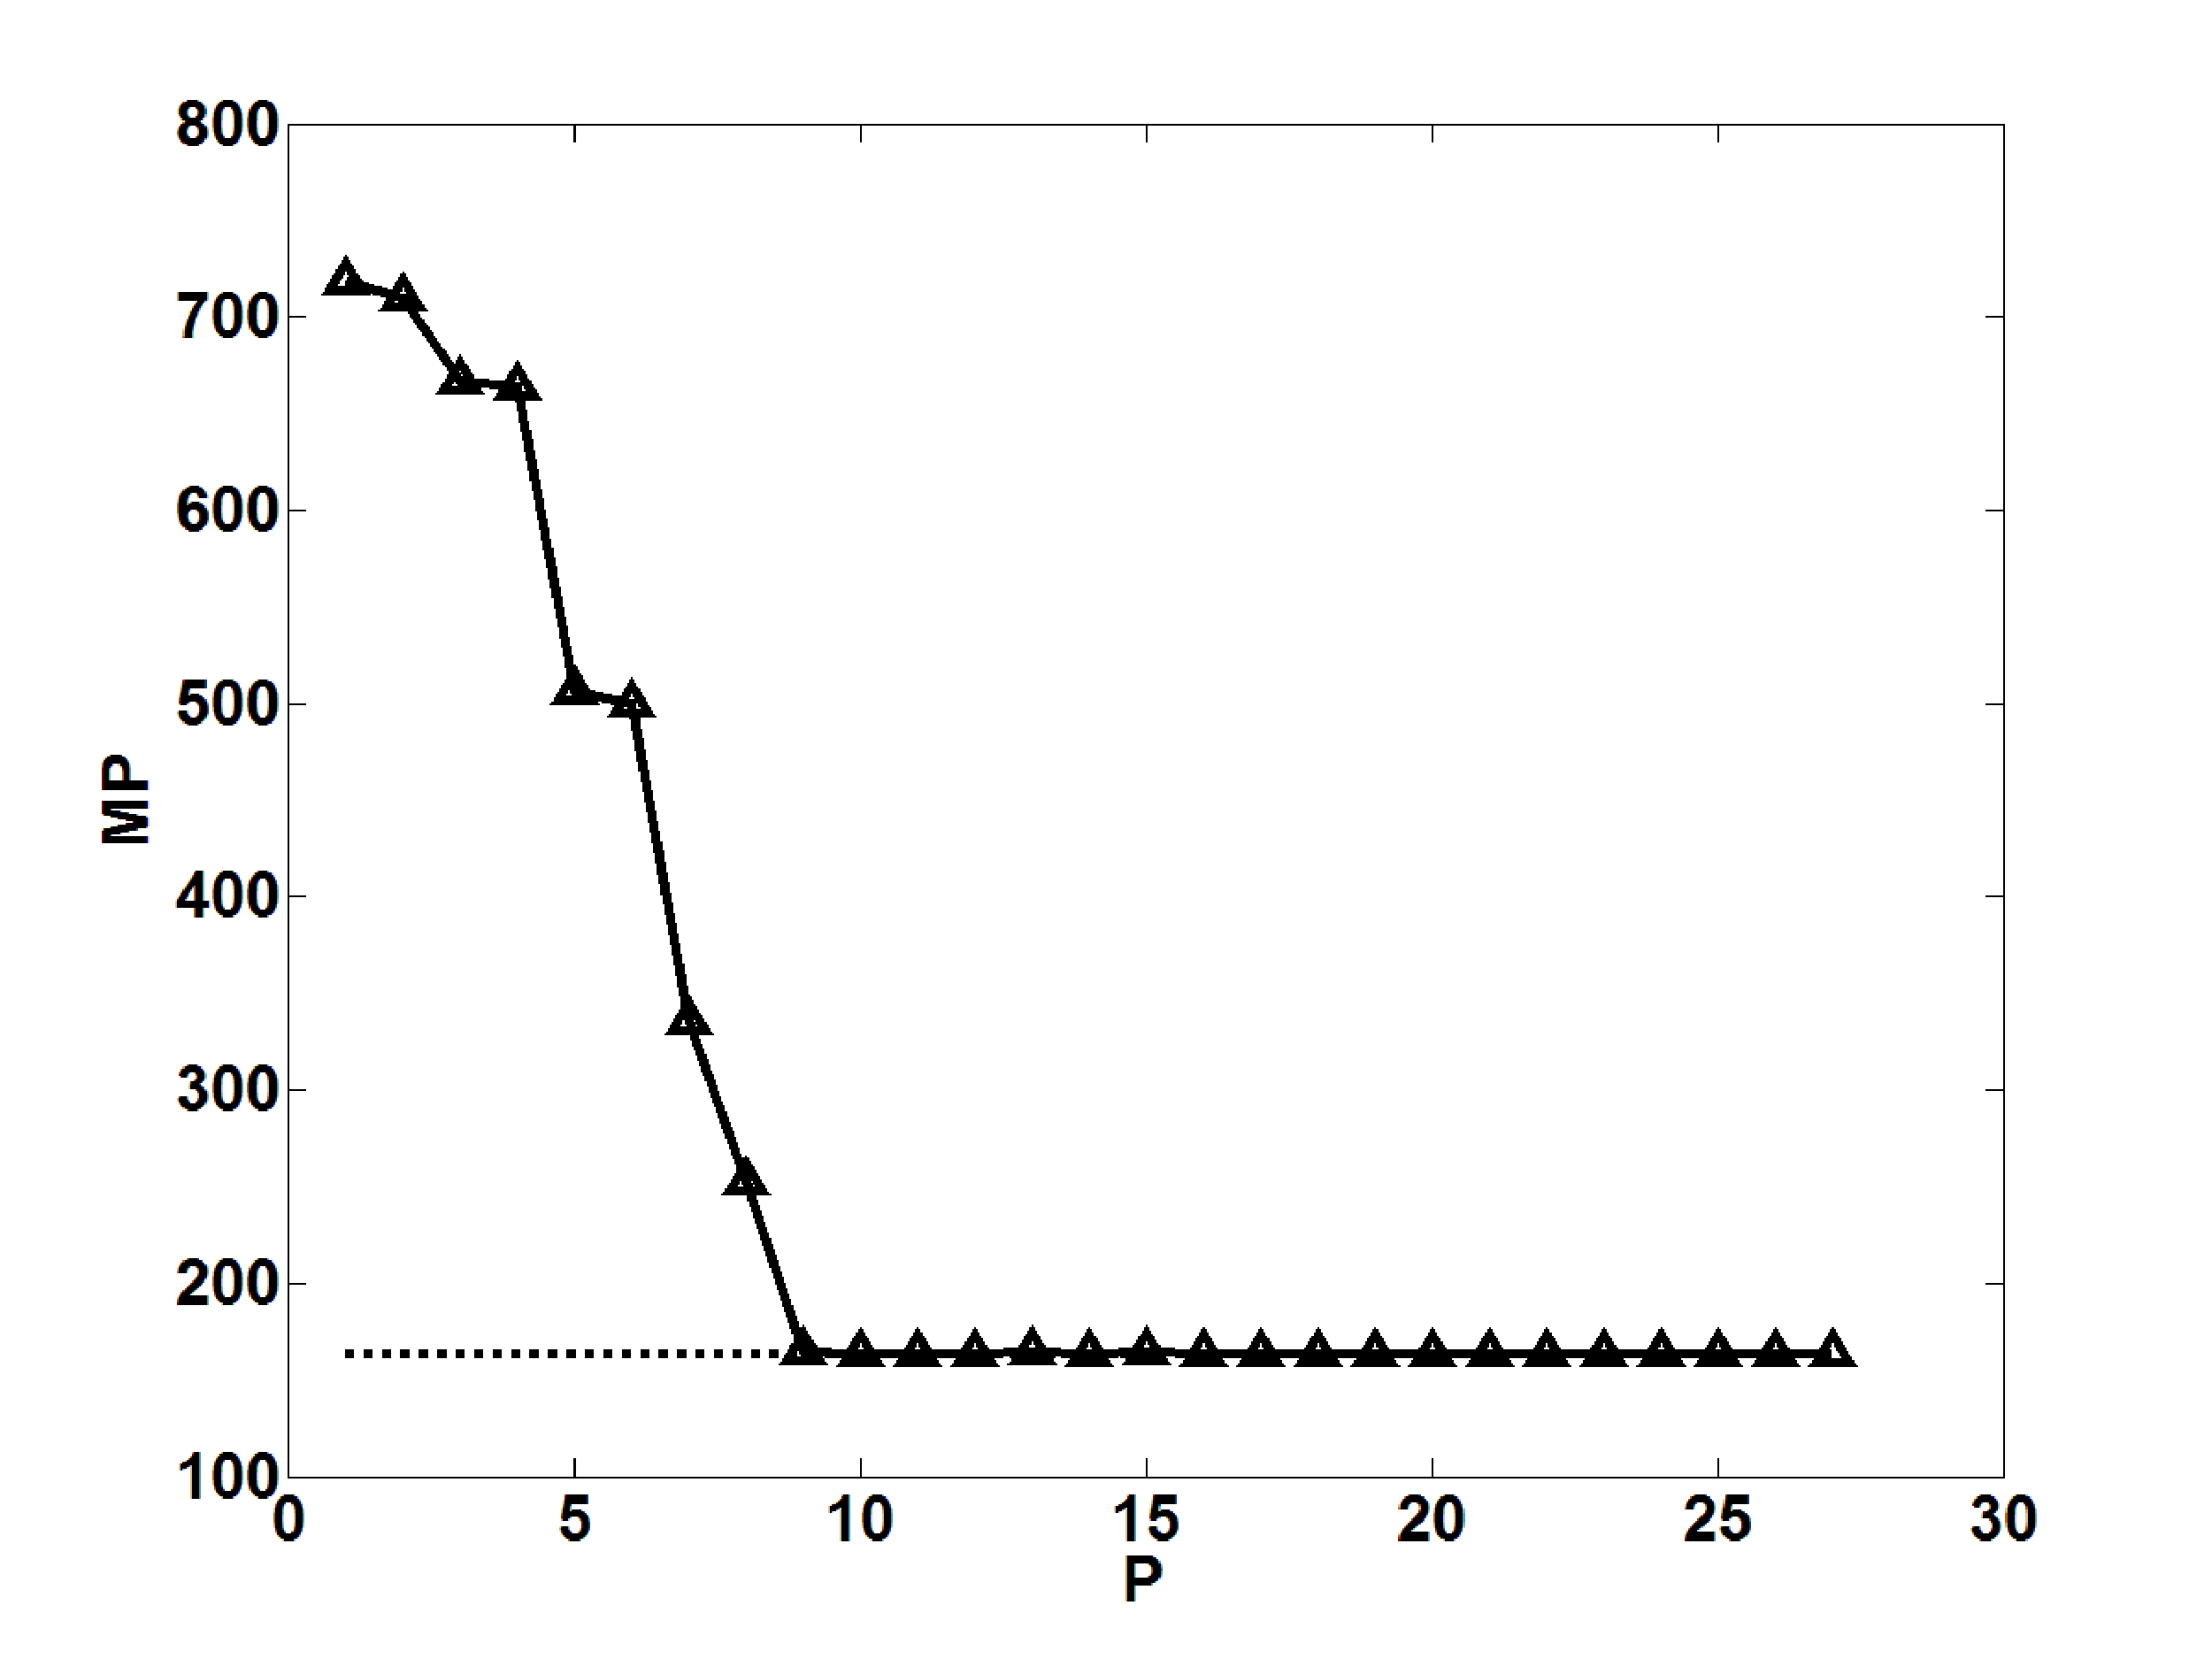
\includegraphics[width=0.3\textwidth]{Miss_parB10}
%	\includegraphics[width=0.3\textwidth]{HvalHbp_parB10}
%	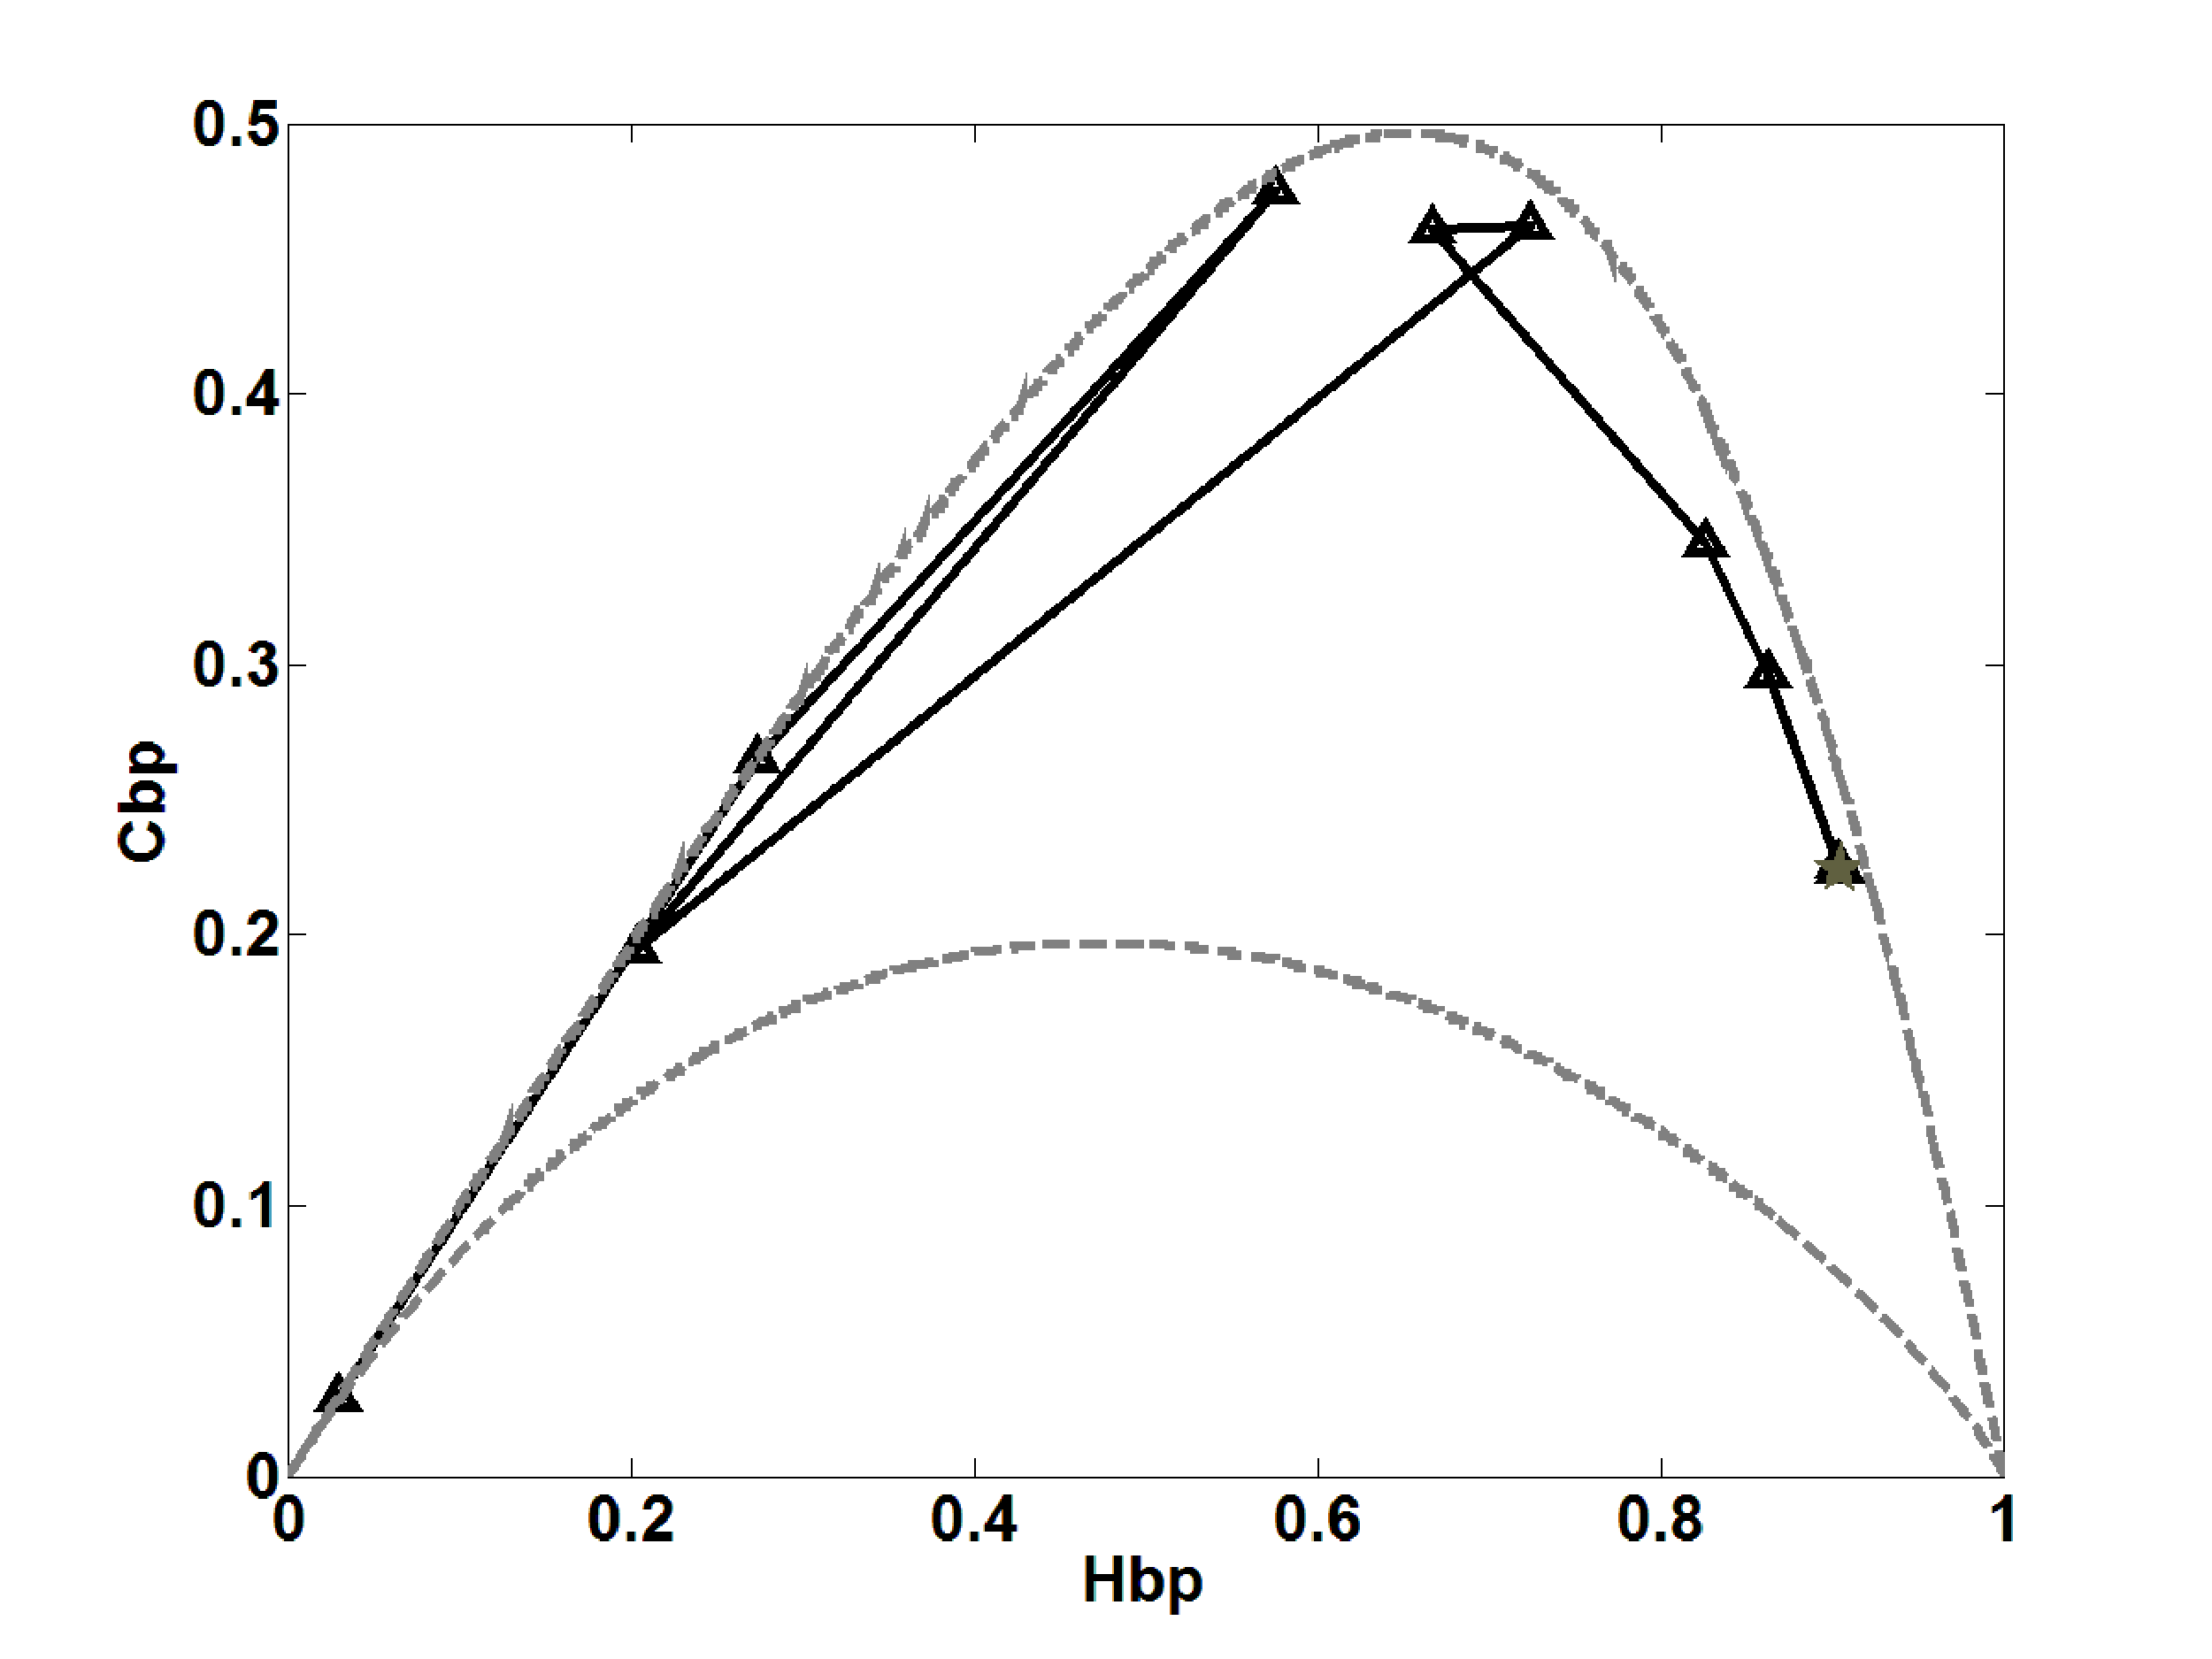
\includegraphics[width=0.3\textwidth]{HbpCbp_parB10}
%	\caption{Statistical properties of EVEN, obtained by skipping the values in the odd position of the time series of  SWITCH,  using decimal representation: (a) $H_{hist}$ vs $P$ (b) $H_{BP}$ vs $P$ (c) $C_{BP}$ vs $P$ (d) Number of missing ordering patterns $MP$ vs $P$. In Figures (a) to (d) dashed line correspond to floating point numbers. (e) representation in the $H_{hist},H_{BP}$ plane in the the decimal numerical system.  The star represents the state for floating points numbers. (f) representation in the $H_{BP},C_{BP}$ plane.  The star represents the state for floating points numbers. } \label{fig:seqpardec}
%\end{figure}

%%%%%%%%%%%%%%%%%%%%%%%%%%%%%%Fig 8.
\begin{figure}
	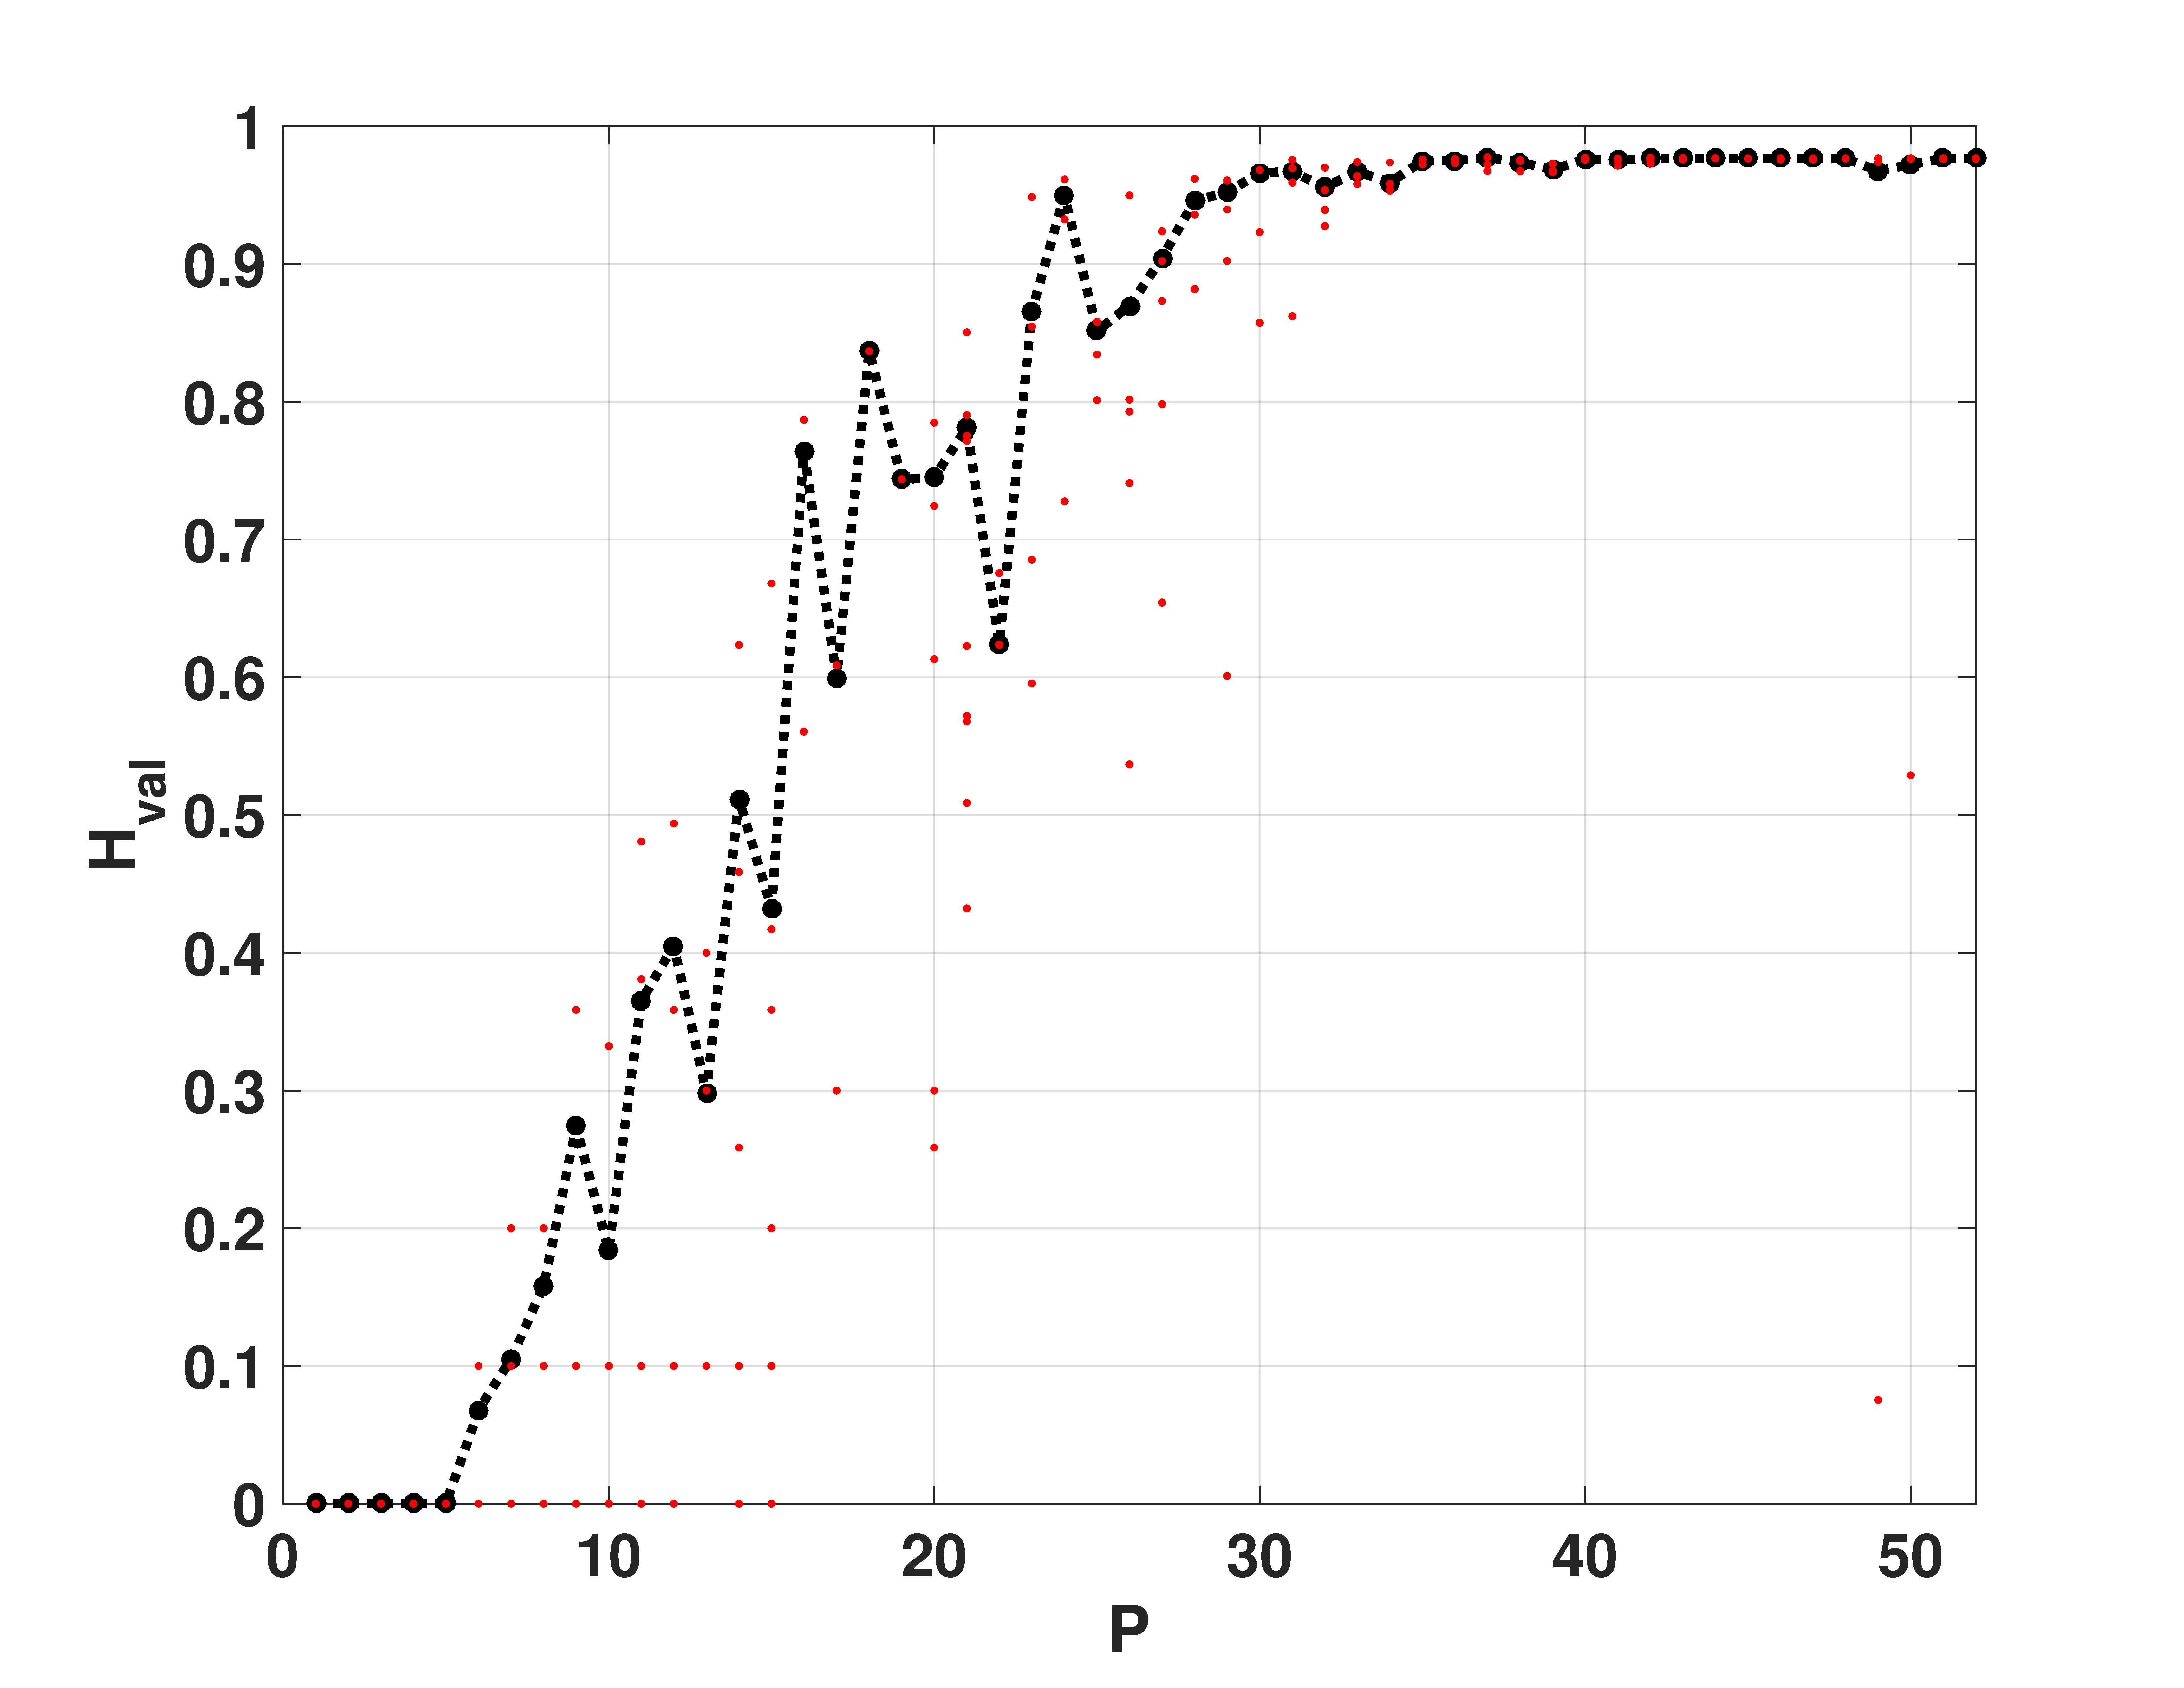
\includegraphics[width=.32\textwidth]{Hval_SwitchB2}
	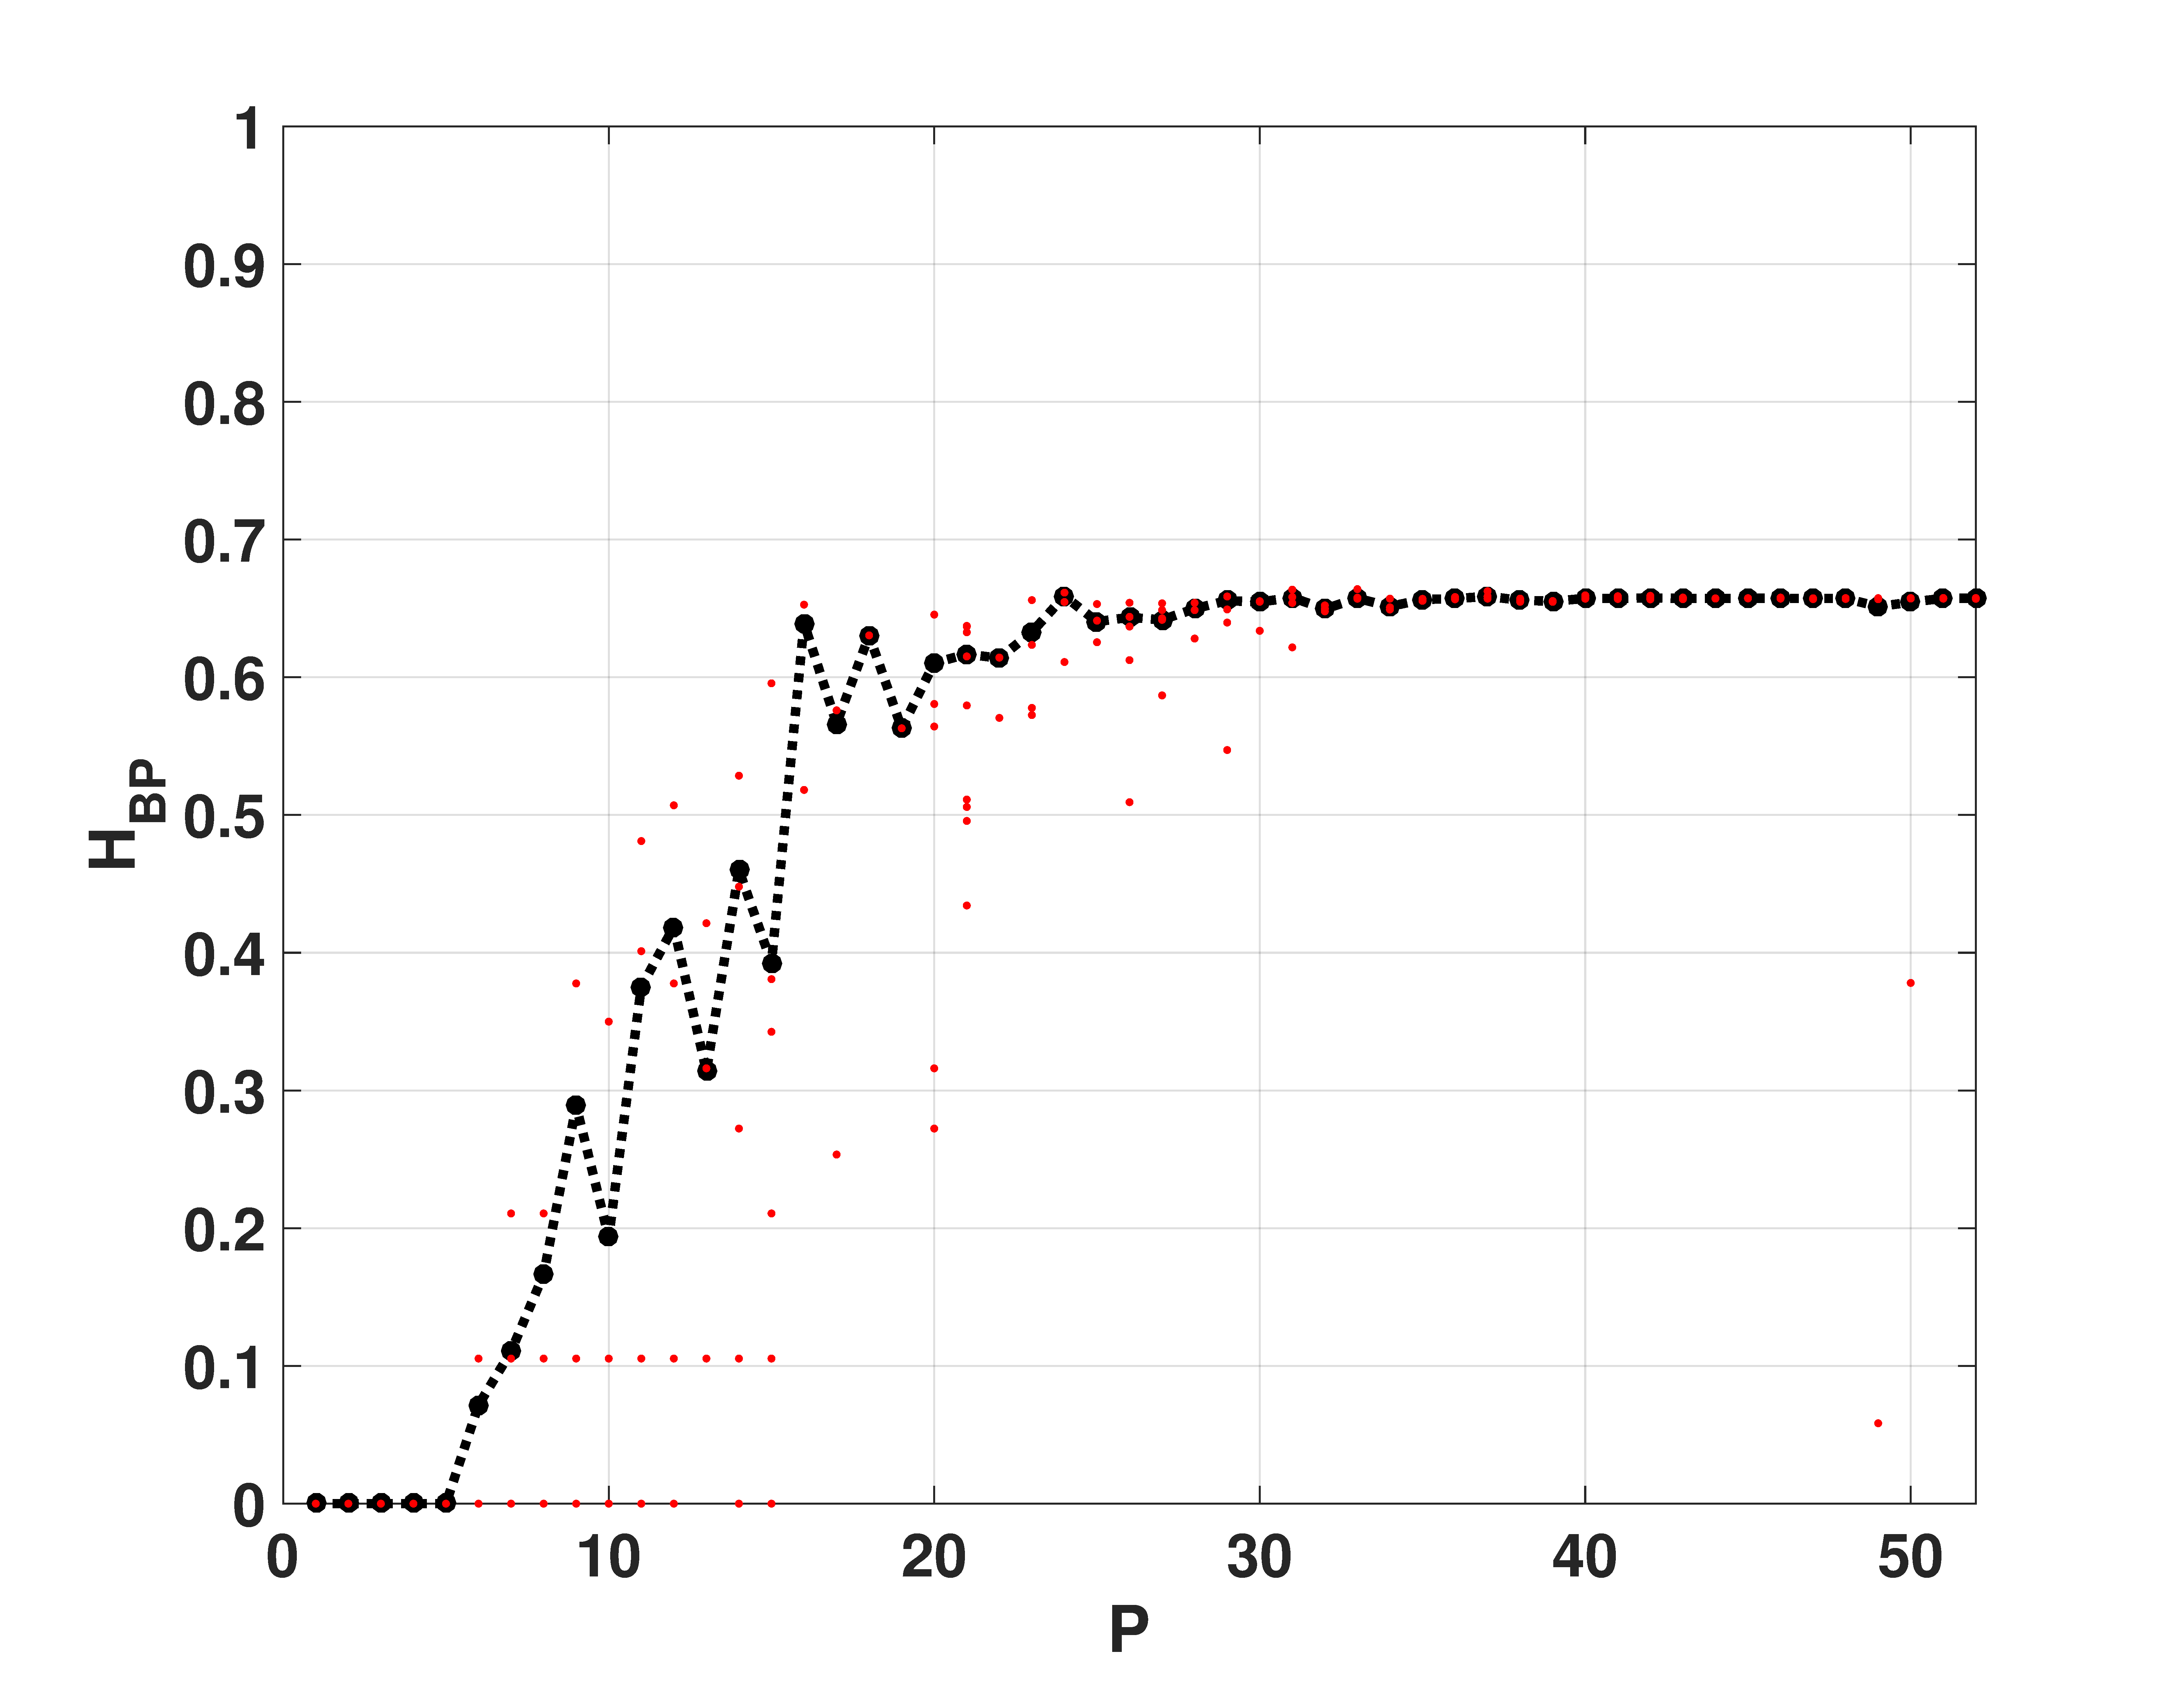
\includegraphics[width=.32\textwidth]{Hbp_SwitchB2}
	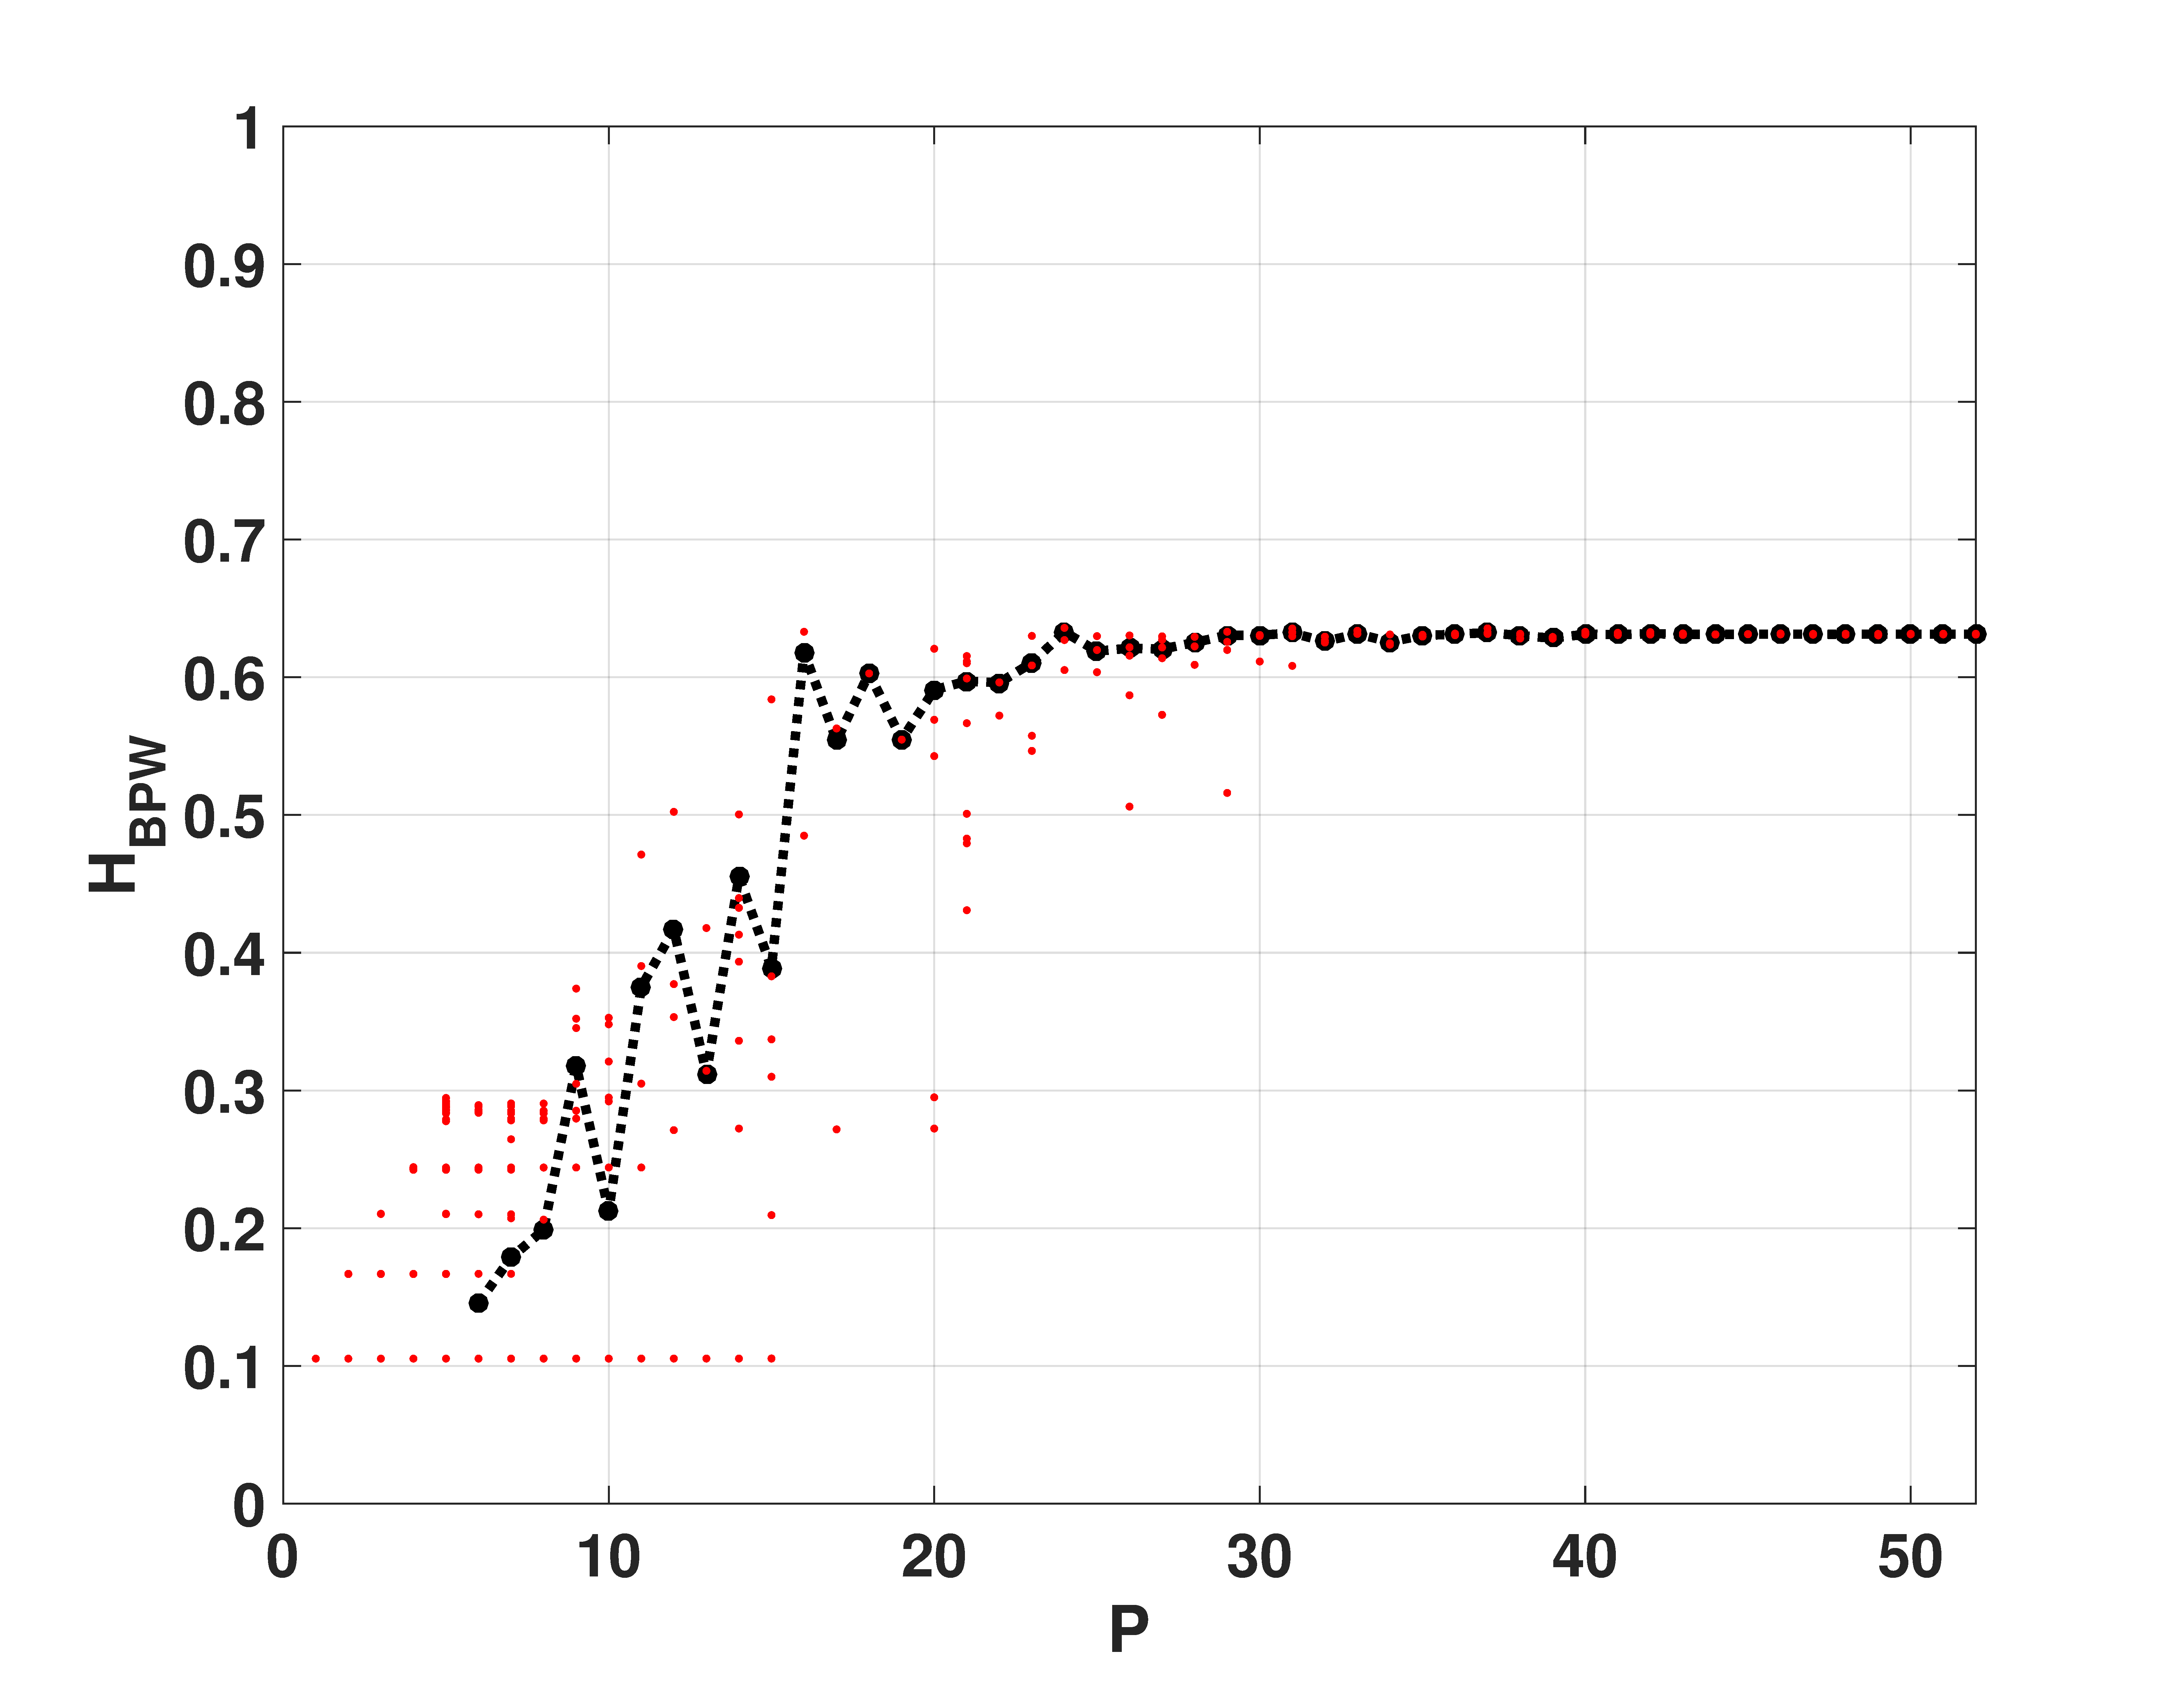
\includegraphics[width=.32\textwidth]{Hbpw_SwitchB2}
	\includegraphics[width=.32\textwidth]{Cbp_SwitchB2}
	\includegraphics[width=.32\textwidth]{Cbpw_SwitchB2}
	\includegraphics[width=.32\textwidth]{MP_SwitchB2}
	\includegraphics[width=.32\textwidth]{Period_SwitchB2}
	\includegraphics[width=.32\textwidth]{HbpHval_SwitchB2}
	\includegraphics[width=.32\textwidth]{HbpwHval_SwitchB2}
	\includegraphics[width=.32\textwidth]{CbpHbp_SwitchB2}
	\includegraphics[width=.32\textwidth]{CbpwHbpw_SwitchB2}
	\caption{Statistical properties of EVEN, obtained by skipping the values in the odd position of the time series of  SWITCH,  using binary representation: (a) $H_{hist}$ vs $P$ (b) $H_{BP}$ vs $P$ (c) $C_{BP}$ vs $P$ (d) Number of missing ordering patterns $MP$ vs $P$. In Figures (a) to (d) dashed line correspond to floating point numbers. (e) representation in the $H_{hist},H_{BP}$ plane in the the binary numerical system.  The star represents the state for floating points numbers. (f) representation in the $H_{BP},C_{BP}$ plane.  The star represents the state for floating points numbers.  } \label{fig:seqparbin}
\end{figure}


%%%%%%%%%%%%%%%%%%%%%%%%%%%% Fig.9
%\begin{figure}
%\includegraphics[width=0.3\textwidth]{Hval_imparB10}
%\includegraphics[width=0.3\textwidth]{Hbp_imparB10}
%\includegraphics[width=0.3\textwidth]{Cbp_imparB10}
%\includegraphics[width=0.3\textwidth]{Miss_imparB10}
%\includegraphics[width=0.3\textwidth]{HvalHbp_imparB10}
%\includegraphics[width=0.3\textwidth]{HbpCbp_imparB10}
%\caption{Statistical properties of EVEN, obtained by skipping the values in the even positions of the time series of  SWITCH,  using decimal representation: (a) $H_{hist}$ vs $P$ (b) $H_{BP}$ vs $P$ (c) $C_{BP}$ vs $P$ d) Number of missing ordering patterns $MP$ vs $P$. In Figures (a) to (d) dashed line correspond to floating point numbers. (e) representation in the $H_{hist},H_{BP}$ plane in the the decimal numerical system.  The star represents the state for floating points numbers. (f) representation in the $H_{BP},C_{BP}$ plane.  The star represents the state for floating points numbers. } \label{fig:seqimpardec}
%\end{figure}

%%%%%%%%%%%%%%%%%%%%%%%%%%%%%%%Fig 10.
\begin{figure}
	\includegraphics[width=.32\textwidth]{Hval_SwitchEvenB2}
	\includegraphics[width=.32\textwidth]{Hbp_SwitchEvenB2}
	\includegraphics[width=.32\textwidth]{Hbpw_SwitchEvenB2}
	\includegraphics[width=.32\textwidth]{Cbp_SwitchEvenB2}
	\includegraphics[width=.32\textwidth]{Cbpw_SwitchEvenB2}
	\includegraphics[width=.32\textwidth]{MP_SwitchEvenB2}
	\includegraphics[width=.32\textwidth]{Period_SwitchEvenB2}
	\includegraphics[width=.32\textwidth]{HbpHval_SwitchEvenB2}
	\includegraphics[width=.32\textwidth]{HbpwHval_SwitchEvenB2}
	\includegraphics[width=.32\textwidth]{CbpHbp_SwitchEvenB2}
	\includegraphics[width=.32\textwidth]{CbpwHbpw_SwitchEvenB2}
\caption{Statistical properties of EVEN, obtained by skipping the values in the odd position of the time series of  SWITCH,  using binary representation: (a) $H_{hist}$ vs $P$ (b) $H_{BP}$ vs $P$ (c) $C_{BP}$ vs $P$ (d) Number of missing ordering patterns $MP$ vs $P$. In Figures (a) to (d) dashed line correspond to floating point numbers. (e) representation in the $H_{hist},H_{BP}$ plane in the the binary numerical system.  The star represents the state for floating points numbers. (f) representation in the $H_{BP},C_{BP}$ plane.  The star represents the state for floating points numbers.  } \label{fig:seqimparbin}
\end{figure}


\begin{figure}
	\includegraphics[width=.32\textwidth]{Hval_SwitchOddB2}
	\includegraphics[width=.32\textwidth]{Hbp_SwitchOddB2}
	\includegraphics[width=.32\textwidth]{Hbpw_SwitchOddB2}
	\includegraphics[width=.32\textwidth]{Cbp_SwitchOddB2}
	\includegraphics[width=.32\textwidth]{Cbpw_SwitchOddB2}
	\includegraphics[width=.32\textwidth]{MP_SwitchOddB2}
	\includegraphics[width=.32\textwidth]{Period_SwitchOddB2}
	\includegraphics[width=.32\textwidth]{HbpHval_SwitchOddB2}
	\includegraphics[width=.32\textwidth]{HbpwHval_SwitchOddB2}
	\includegraphics[width=.32\textwidth]{CbpHbp_SwitchOddB2}
	\includegraphics[width=.32\textwidth]{CbpwHbpw_SwitchOddB2}
	\caption{Statistical properties of EVEN, obtained by skipping the values in the odd position of the time series of  SWITCH,  using binary representation: (a) $H_{hist}$ vs $P$ (b) $H_{BP}$ vs $P$ (c) $C_{BP}$ vs $P$ (d) Number of missing ordering patterns $MP$ vs $P$. In Figures (a) to (d) dashed line correspond to floating point numbers. (e) representation in the $H_{hist},H_{BP}$ plane in the the binary numerical system.  The star represents the state for floating points numbers. (f) representation in the $H_{BP},C_{BP}$ plane.  The star represents the state for floating points numbers.  } \label{fig:seqimparbin}
\end{figure}
%%%%%%%%%%%%%%%%%%%%%%%%%%% Fig.11
%\center
%\begin{figure}
%	\includegraphics[width=0.8\textwidth]{MeanPeriod_logisticoB10}
%	\caption{Period $T$ as a function of de number of decimal digits $P$ for the LOG map.} \label{fig:perio}
%\end{figure}